%
% $RCSfile: logical_architecture.tex,v $
%
% Copyright (C) 2002-2008. Christian Heller.
%
% Permission is granted to copy, distribute and/or modify this document
% under the terms of the GNU Free Documentation License, Version 1.1 or
% any later version published by the Free Software Foundation; with no
% Invariant Sections, with no Front-Cover Texts and with no Back-Cover
% Texts. A copy of the license is included in the section entitled
% "GNU Free Documentation License".
%
% http://www.cybop.net
% - Cybernetics Oriented Programming -
%
% http://www.resmedicinae.org
% - Information in Medicine -
%
% Version: $Revision: 1.1 $ $Date: 2008-08-19 20:41:07 $ $Author: christian $
% Authors: Christian Heller <christian.heller@tuxtax.de>
%

\chapter{Logical Architecture}
\label{logical_architecture_heading}
\index{Logical Architecture}
\index{Inside of a Software System}
\index{Layers}
\index{Presentation Layer}
\index{Domain Layer}
\index{Data Source Layer}
\index{Physical Tiers}
\index{Object Oriented Programming}
\index{OOP}
\index{Unified Modeling Language}
\index{UML}
\index{Computer Language}
\index{Programming Paradigms}
\index{Patterns}
\index{Framework}
\index{Component}
\index{Ontology}
\index{Statics, Terms and Synonyms}
\index{State, Terms and Synonyms}
\index{Logic, Terms and Synonyms}
\index{Dynamics, Terms and Synonyms}
\index{Structure, Terms and Synonyms}

\begin{flushright}
    \textsl{
        Because nothing is more difficult and\\
        nothing requires more Personality,\\
        than to be in open Opposition to current Time\\
        and loudly to say: NO.
    }\\
    \textsc{Kurt Tucholsky}
\end{flushright}

While the previous chapter had a look at the \emph{Physical Architecture} of an
IT environment, that is the systems and their communication, this chapter will
discuss the \emph{Logical Architecture}, that is the \emph{Inside} of a software
system.

The program source code of every system is -- or at least should be -- separated
into logical parts like \emph{Layers}, for example (figure \ref{logical_figure}).
Current systems distinguish \emph{Presentation-}, \emph{Domain-} and
\emph{Data Source} layer \cite{fowler2002}. Each of them contains functionality
for a specific task: the presentation layer for user interaction; the domain for
business logic; the data source for database communication.

\begin{figure}[ht]
    \begin{center}
        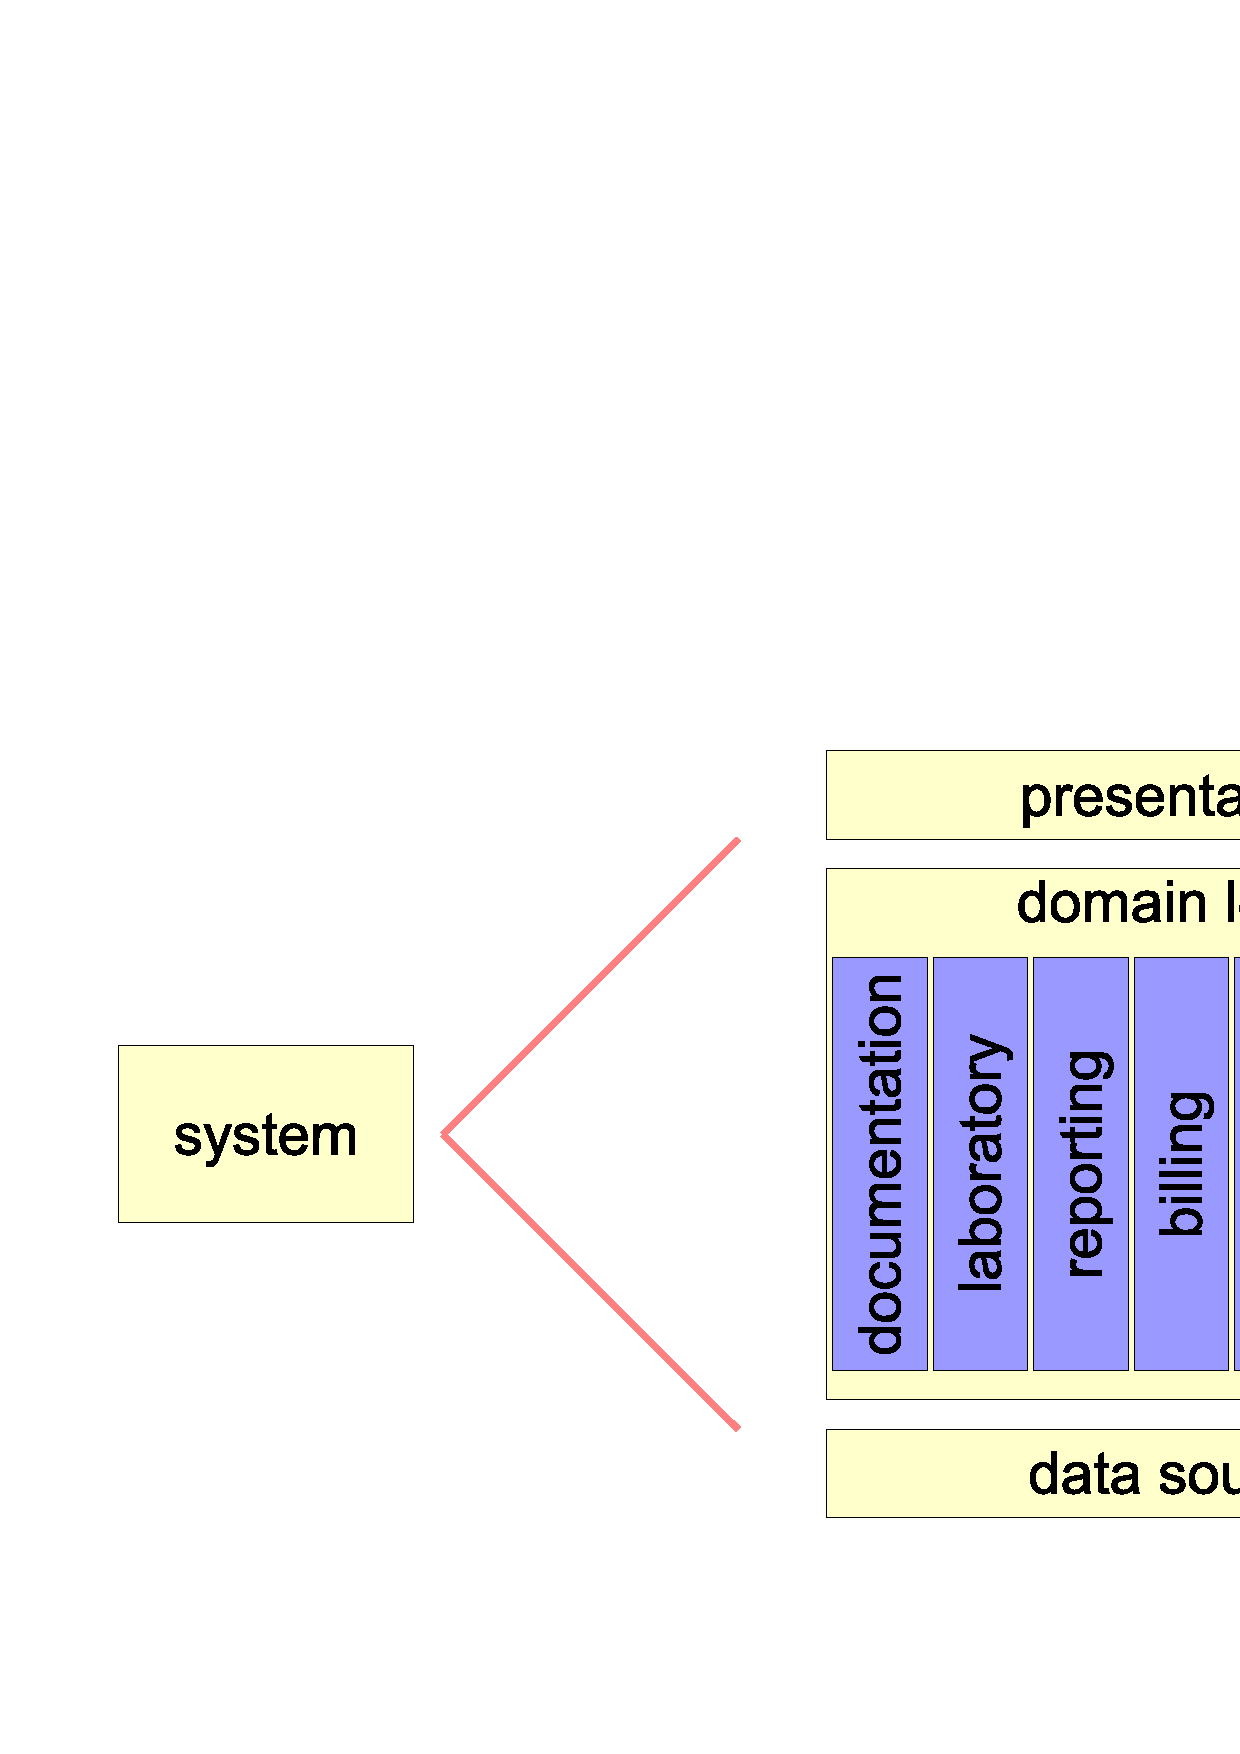
\includegraphics[scale=0.3,angle=-90]{graphic/logical.pdf}
        \caption{System with Logical Layers}
        \label{logical_figure}
    \end{center}
\end{figure}

Just like physical tiers can be scaled vertically and horizontally, the logical
layers within a software system can be shared in a similar way. Figure
\ref{logical_figure} splits the horizontal business logic layer of a healthcare
environment into the vertical domains \emph{Documentation}, \emph{Laboratory},
\emph{Reporting}, \emph{Billing}, \emph{Administration}, \emph{Imaging},
\emph{Devices}.

One must not mix logical layers with the physical tiers that were introduced in
chapter \ref{physical_architecture_heading}! It is true, logical layers may be
distributed to physically separated systems -- the presentation layer, for
example, may be situated on the physical client tier (frontend). But as section
\ref{misleading_tiers_heading} pointed out: In the end, \emph{all}
systems (not only the client tier) will have to interact with users and further
systems in some way and thus cannot only implement one functionality but need
to be able to communicate \emph{universally}. More on that in part
\ref{contribution_heading}.

Layers are just one concept aiming to improve a system's architecture. There
are many more. The introduction of \emph{Object Oriented Programming} (OOP) and
the \emph{Unified Modeling Language} (UML), for example, animated and enabled
software developers to structure their program code more and more clearly.
\emph{Patterns}, \emph{Frameworks}, \emph{Components} and \emph{Ontologies} are
further techniques which delivered many new concepts and solutions. They all
represent the state-of-the-art in software design and will be investigated
together with their \emph{Pros} and \emph{Cons} in the following sections. The
most general concepts, however, are still provided by computer languages and
programming paradigms, which is why they are described first.

Over the years, several terms and synonyms describing architectural elements
were introduced. Following are some examples, grouped arbitrarily into those
that represent a kind of \emph{State} and others that manipulate states
according to certain rules of \emph{Logic}. Both will be called \emph{Statics},
later in this work (parts \ref{contribution_heading} and \ref{proof_heading}).
Besides these, there are terms for elements that describe the runtime behaviour
of a system -- its \emph{Dynamics}, and others for some \emph{Structural}
elements. They all appear in one form or another in the following sections.

\begin{itemize}
    \item[-] Statics:
    \begin{itemize}
        \item[-] State: Operand, Data, Value, Parameter, Attribute
        \item[-] Logic: Operation, Operator, Function, Procedure, Method,
            Algorithm, Activity, Workflow
    \end{itemize}
    \item[-] Dynamics: Allocated Memory, Array, Instance, Object, Property,
        Process, Signal, Event, Action
    \item[-] Structure: Class, Component, Module, Library, Package, Layer
\end{itemize}

%
% $RCSfile: paradigm_and_language.tex,v $
%
% Copyright (C) 2002-2008. Christian Heller.
%
% Permission is granted to copy, distribute and/or modify this document
% under the terms of the GNU Free Documentation License, Version 1.1 or
% any later version published by the Free Software Foundation; with no
% Invariant Sections, with no Front-Cover Texts and with no Back-Cover
% Texts. A copy of the license is included in the section entitled
% "GNU Free Documentation License".
%
% http://www.cybop.net
% - Cybernetics Oriented Programming -
%
% http://www.resmedicinae.org
% - Information in Medicine -
%
% Version: $Revision: 1.1 $ $Date: 2008-08-19 20:41:08 $ $Author: christian $
% Authors: Christian Heller <christian.heller@tuxtax.de>
%

\section{Paradigm and Language}
\label{paradigm_and_language_heading}
\index{Paradigm and Language}
\index{Computer Language}
\index{Programming Language}
\index{Markup Language}
\index{Data Manipulation Language}
\index{DML}
\index{Page Description Language}
\index{Specification Language}

Manifold instructions exist that allow humans to program a computer. A set of
such instructions is called \emph{Programming Language} and is one of many
groups of different \emph{Computer Languages}. Other groups are for example
\emph{Markup Languages}, \emph{Data Manipulation Languages} (DML),
\emph{Page Description Languages} or \emph{Specification Languages}
\cite{wikipedia}.

%
% $RCSfile: language_history.tex,v $
%
% Copyright (C) 2002-2008. Christian Heller.
%
% Permission is granted to copy, distribute and/or modify this document
% under the terms of the GNU Free Documentation License, Version 1.1 or
% any later version published by the Free Software Foundation; with no
% Invariant Sections, with no Front-Cover Texts and with no Back-Cover
% Texts. A copy of the license is included in the section entitled
% "GNU Free Documentation License".
%
% http://www.cybop.net
% - Cybernetics Oriented Programming -
%
% http://www.resmedicinae.org
% - Information in Medicine -
%
% Version: $Revision: 1.1 $ $Date: 2008-08-19 20:41:07 $ $Author: christian $
% Authors: Christian Heller <christian.heller@tuxtax.de>
%

\subsection{Language History}
\label{language_history_heading}
\index{Language History}
\index{Programming Paradigm}
\index{Computer Languages Timeline}
\index{Language List}
\index{Programming Language Generations}

Just as a software engineering school advocates its very own \emph{Methodology}
(chapter \ref{software_engineering_process_heading}), each programming language
advocates a special \emph{Programming Paradigm} \cite{wikipedia} (sometimes
also more than one). Some efforts categorise languages or their paradigms
historically \cite{steppan}. Eric Levenez' \emph{Computer Languages Timeline}
\cite{levenez} captures common programming languages from a historical
perspective. Some of them are shown in the simplified figure
\ref{language_figure} (whose columns have no meaning). A much more
comprehensive overview listing more than 2500 languages is given in the
\emph{Language List} \cite{kinnersley} of Bill Kinnersley.

\begin{figure}[ht]
    \begin{center}
        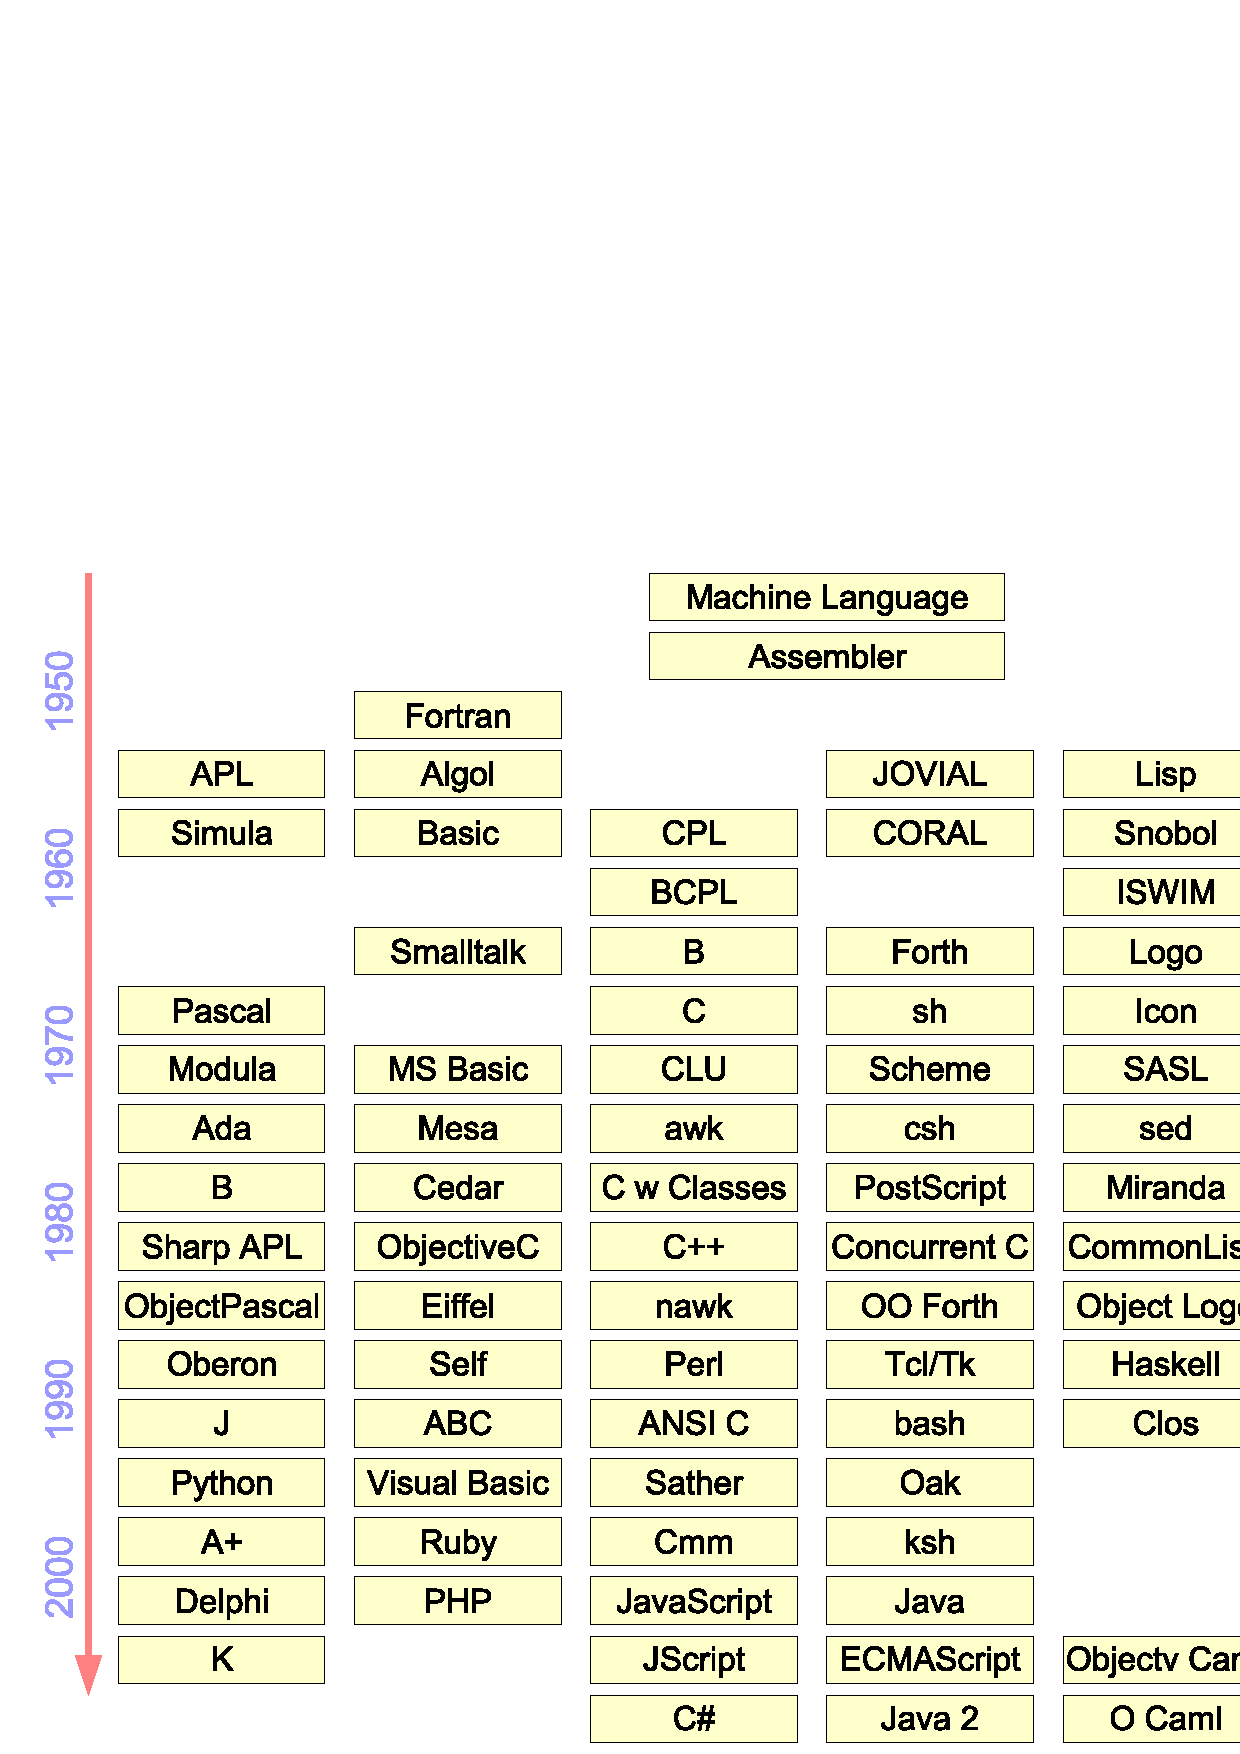
\includegraphics[scale=0.3,angle=-90]{graphic/language.pdf}
        \caption{Programming Language History}
        \label{language_figure}
    \end{center}
\end{figure}

A lineage can be identified for every language, some popular of which are shown
in the following list, the corresponding language name mentioned at first,
being followed by the names of the language's ancestors. The right-most
language represents the oldest ancestor. Only \emph{one} lineage of arbitrary
choice is considered for each language; most languages have \emph{further}
ancestors that are not mentioned here:

\begin{itemize}
    \item[-] \emph{Java 2:} Java 1, Oak, Cedar, Mesa, Algol, IAL, Fortran
    \item[-] \emph{C\#:} C++, C with Classes, C, B, BCPL, CPL, Algol
    \item[-] \emph{VB.NET:} Visual Basic, MS Basic, Basic, Algol
    \item[-] \emph{Delphi:} Object Pascal, Pascal, Algol
    \item[-] \emph{Oberon:} Modula, Pascal
    \item[-] \emph{Self:} Smalltalk, Simula, Algol
    \item[-] \emph{Tcl/Tk:} Tcl
    \item[-] \emph{Python:} ABC, B
    \item[-] \emph{Perl:} nawk, awk, Icon, Snobol
    \item[-] \emph{PHP:} PHP/FI, Perl
    \item[-] \emph{Ruby:} CLU, Pascal
    \item[-] \emph{Haskell:} Miranda, KRC, SASL, ISWIM
    \item[-] \emph{O Caml:} Objective Caml, Caml, SML, ML
    \item[-] \emph{OO COBOL:} COBOL, Flow-Matic, B-O
    \item[-] \emph{NetRexx:} Object Rexx, Rexx, Rex, PL/1 ANS, PL/M, PL/I, COBOL
    \item[-] \emph{Open M:} M, MUMPS
    \item[-] \emph{Scheme:} Common Lisp, Lisp
    \item[-] \emph{PostScript:} OO Forth, Forth
\end{itemize}

Other historical approaches assign each programming language to a special
\emph{Generation}. Commonly used programming language generations and some of
their representatives are shown following \cite{wikipedia}:

\begin{itemize}
    \item[-] \emph{First Generation Language}: machine-level language
    \item[-] \emph{Second Generation Language}: assembly language
    \item[-] \emph{Third Generation Language} (3GL): Fortran, Algol, COBOL, Basic, C, C++
    \item[-] \emph{Fourth Generation Language} (4GL): SQL, Mathematica, SAS, VB, MATLAB
    \item[-] \emph{Fifth Generation Language}: Prolog, OPS5, Mercury
\end{itemize}

%
% $RCSfile: paradigm_overview.tex,v $
%
% Copyright (C) 2002-2008. Christian Heller.
%
% Permission is granted to copy, distribute and/or modify this document
% under the terms of the GNU Free Documentation License, Version 1.1 or
% any later version published by the Free Software Foundation; with no
% Invariant Sections, with no Front-Cover Texts and with no Back-Cover
% Texts. A copy of the license is included in the section entitled
% "GNU Free Documentation License".
%
% http://www.cybop.net
% - Cybernetics Oriented Programming -
%
% http://www.resmedicinae.org
% - Information in Medicine -
%
% Version: $Revision: 1.1 $ $Date: 2008-08-19 20:41:08 $ $Author: christian $
% Authors: Christian Heller <christian.heller@tuxtax.de>
%

\subsection{Paradigm Overview}
\label{paradigm_overview_heading}
\index{Paradigm Overview}
\index{Programming Paradigm Systematics}
\index{Imperative (Command Oriented) Programming Language}
\index{Declarative Programming Language}
\index{Machine Language}
\index{Assembly Language}
\index{System Programming}
\index{Functional Programming}
\index{Logical Programming}
\index{Scripting Language}
\index{Typeless Programming}
\index{Structured- and Procedural Programming}
\index{SPP}
\index{Object Oriented Programming}
\index{OOP}
\index{Programming Paradigms as Contrasting Pairs}

Several other systematics, besides the historical one shown in the previous
section, exist to categorise programming languages and their paradigms. Some
authors, for example, divide computer languages into those that have to be
compiled before being executed and those which are interpreted at runtime.
Figure \ref{paradigm_figure} shows yet another arbitrary, tree-like systematics
that was assembled on the basis of \cite{wikipedia} and \cite{kinnersley}.

\begin{figure}[ht]
    \begin{center}
        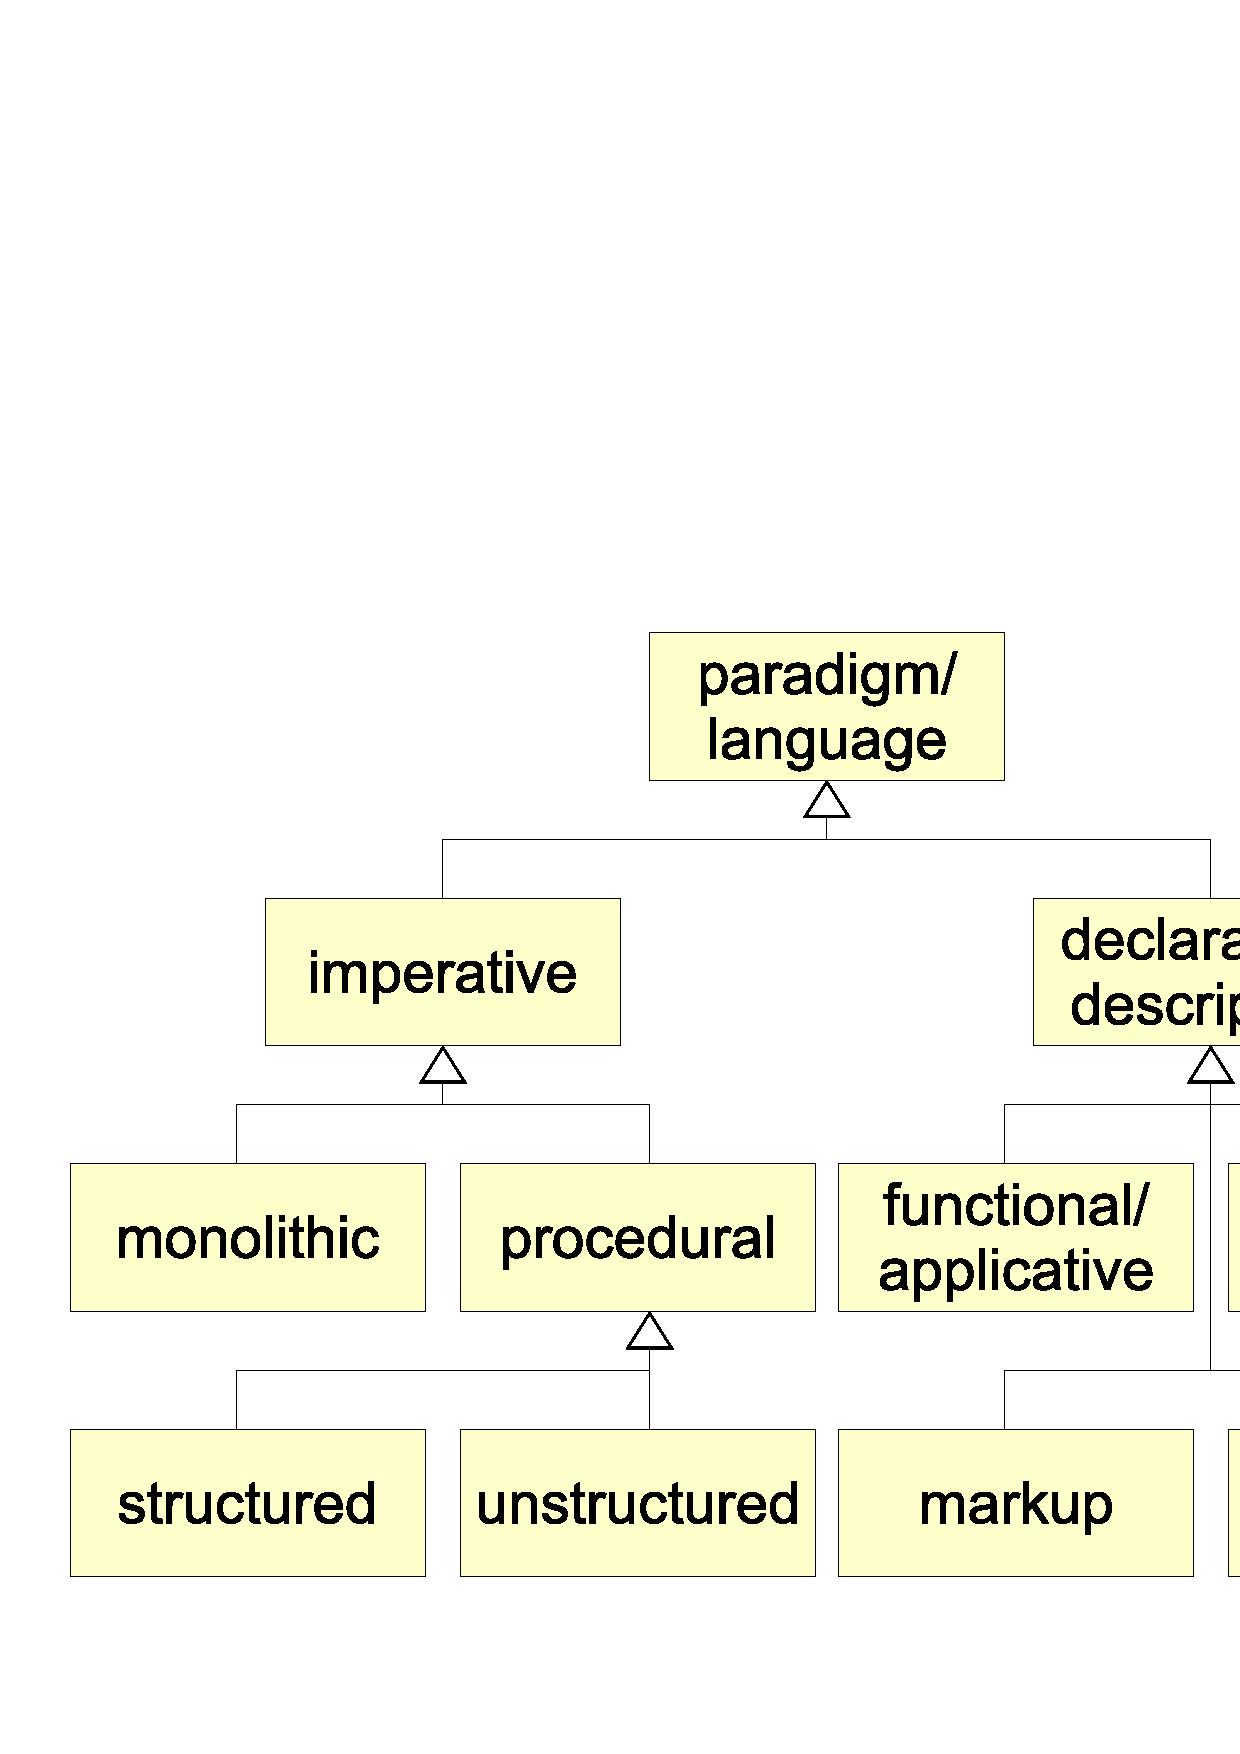
\includegraphics[scale=0.3,angle=-90]{graphic/paradigm.pdf}
        \caption{Programming Paradigm Systematics}
        \label{paradigm_figure}
    \end{center}
\end{figure}

\emph{Machine-} and \emph{Assembly Language} as well as \emph{System Programming}
are \emph{imperative} (command-oriented). \emph{Functional-} and
\emph{Logical Programming}, on the other hand, are \emph{declarative}, just as
most \emph{Scripting Languages} used for \emph{Typeless Programming}. The
boundaries tend to be vague, however. Many of the new languages borrow features
from more than one programming paradigm. Similarly, the concepts of
\emph{Structured and Procedural Programming} (SPP) and
\emph{Object Oriented Programming} (OOP) are not only used in system
programming-, but also in scripting languages.

It is important to note that it is extremely difficult, if not impossible, to
arrange all programming languages into just one tree of categories. Kinnersley
\cite{kinnersley} writes that \textit{for every classification scheme there
will be a large proportion of languages that do not fit \ldots\ most languages
are not purely one or the other}. The \emph{Logo} language, for example, is an
adaptation of the functional language \emph{Lisp}, that is non-imperative, yet
procedural \cite{wikipedia}. Figure \ref{paradigm_figure} can therefore only be
seen as trial to create a systematics of the most common programming paradigms.
In order to avoid miscategorisation, the Wikipedia Encyclopedia \cite{wikipedia}
prefers to list programming paradigms as contrasting pairs, for example:

\begin{itemize}
    \item[-] Procedural vs. Functional
    \item[-] Imperative vs. Declarative
    \item[-] Structured vs. Unstructured
    \item[-] Value-level vs. Function-level
    \item[-] Flow-driven vs. Event-driven
    \item[-] Scalar vs. Array
    \item[-] Class-based vs. Prototype-based
    \item[-] Rule-based vs. Constraint
\end{itemize}

Not all items of the list are explained in this work since this would break its
frame and focus. However, some of the most important programming language
concepts in use today are described in the following sections.

%
% $RCSfile: hardware_architecture.tex,v $
%
% Copyright (C) 2002-2008. Christian Heller.
%
% Permission is granted to copy, distribute and/or modify this document
% under the terms of the GNU Free Documentation License, Version 1.1 or
% any later version published by the Free Software Foundation; with no
% Invariant Sections, with no Front-Cover Texts and with no Back-Cover
% Texts. A copy of the license is included in the section entitled
% "GNU Free Documentation License".
%
% http://www.cybop.net
% - Cybernetics Oriented Programming -
%
% http://www.resmedicinae.org
% - Information in Medicine -
%
% Version: $Revision: 1.1 $ $Date: 2008-08-19 20:41:07 $ $Author: christian $
% Authors: Christian Heller <christian.heller@tuxtax.de>
%

\subsection{Hardware Architecture}
\label{hardware_architecture_heading}
\index{Hardware Architecture}
\index{Abstract Levels of a Virtual Machine}
\index{Virtual Machine}
\index{VM}
\index{Computer Structure}
\index{Lower Levels of a Computer Structure}
\index{Higher Levels of a Computer Structure}
\index{Problem Oriented Languages}
\index{POL}

In his very clear book, Tanenbaum \cite{tanenbaum1999} organises instructions
in abstract \emph{Levels} (figure \ref{vm_figure}), which he also calls
\emph{Virtual Machines} (VM), since each level could be seen as hypothetic
computer with an own language. Further on, he considers hardware and software
to be \textit{logically equivalent} because one could replace the other.

\begin{figure}[ht]
    \begin{center}
        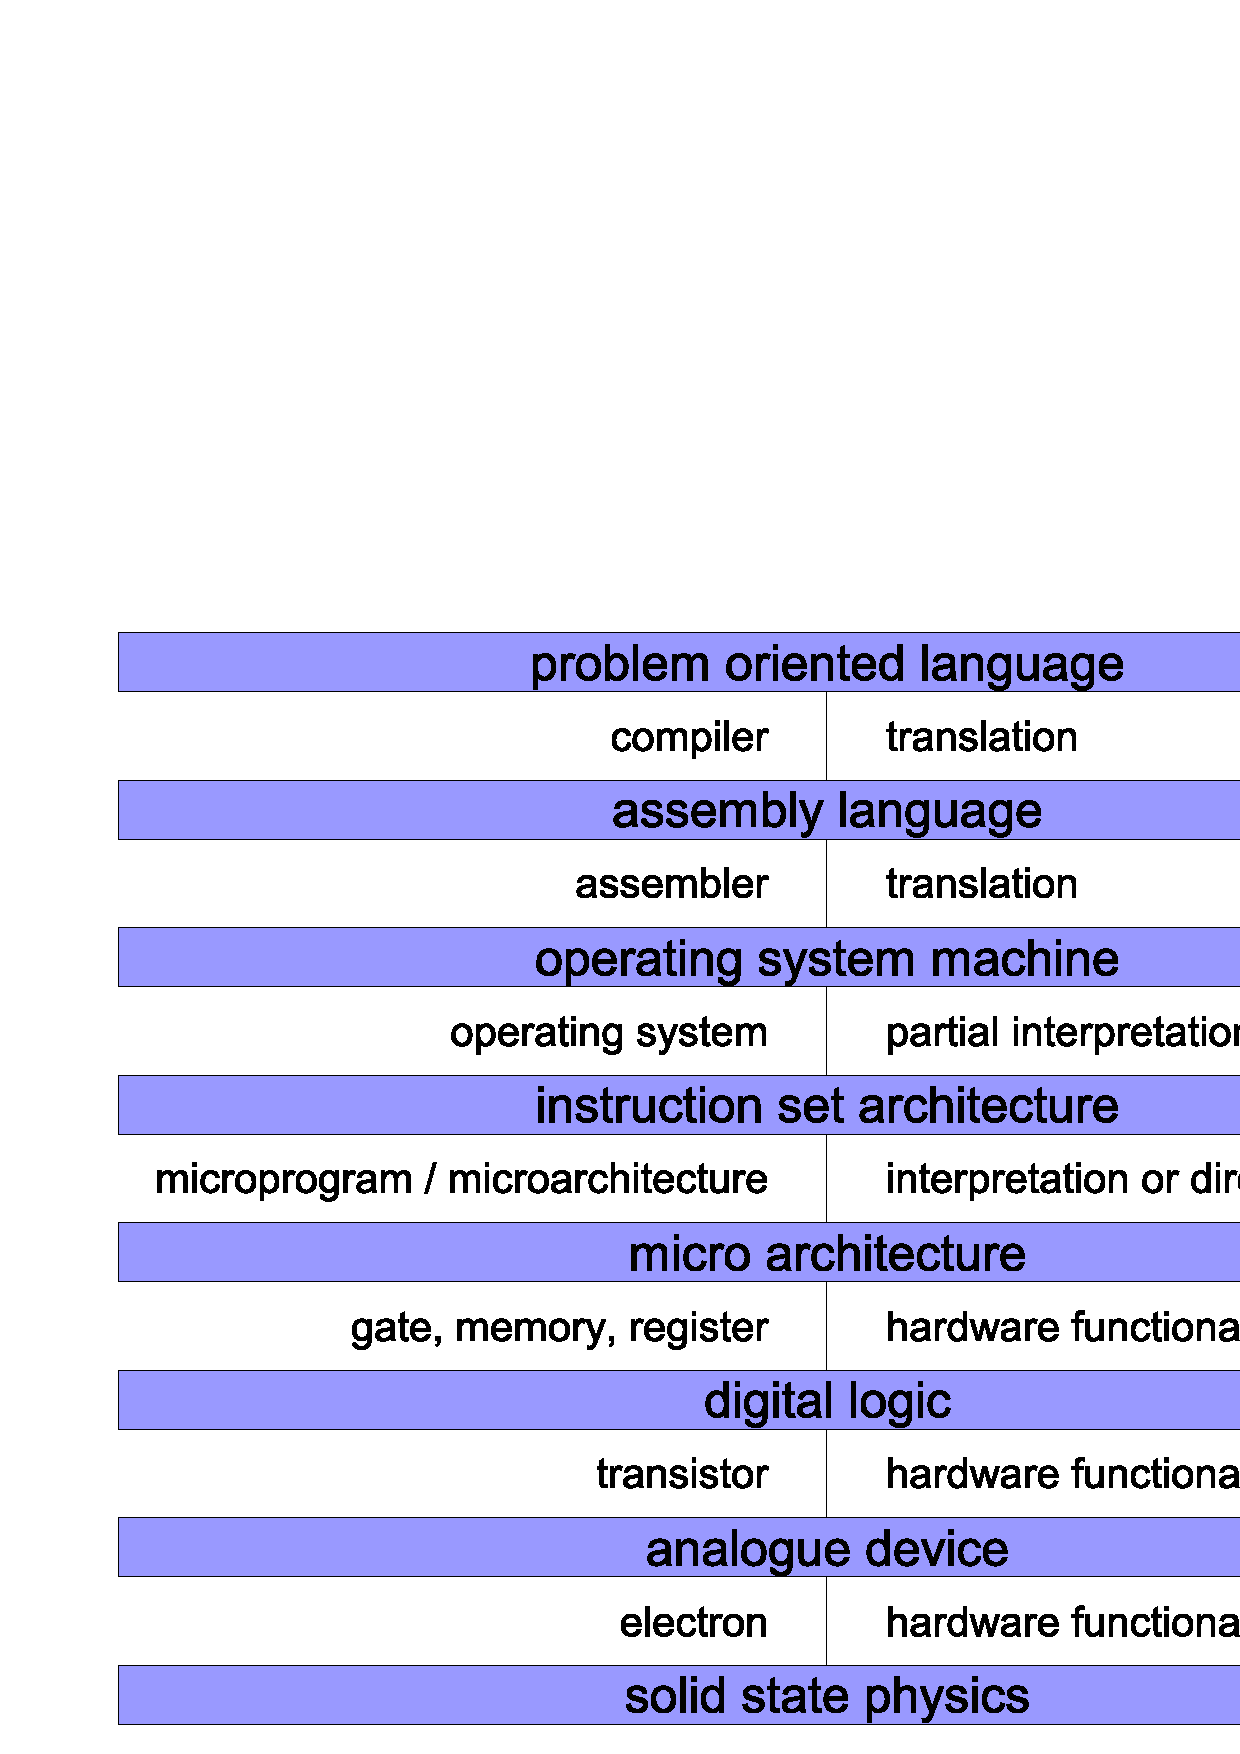
\includegraphics[scale=0.3,angle=-90]{graphic/vm.pdf}
        \caption{Computer Structure (adapted from \cite{tanenbaum1999})}
        \label{vm_figure}
    \end{center}
\end{figure}

The next sub sections are based on this structure. They describe lower levels,
close to hardware. Later sections then place more emphasis on concepts
introduced by higher-level \emph{Problem Oriented Languages} (POL).

%
% $RCSfile: digital_logic.tex,v $
%
% Copyright (C) 2002-2008. Christian Heller.
%
% Permission is granted to copy, distribute and/or modify this document
% under the terms of the GNU Free Documentation License, Version 1.1 or
% any later version published by the Free Software Foundation; with no
% Invariant Sections, with no Front-Cover Texts and with no Back-Cover
% Texts. A copy of the license is included in the section entitled
% "GNU Free Documentation License".
%
% http://www.cybop.net
% - Cybernetics Oriented Programming -
%
% http://www.resmedicinae.org
% - Information in Medicine -
%
% Version: $Revision: 1.1 $ $Date: 2008-08-19 20:41:06 $ $Author: christian $
% Authors: Christian Heller <christian.heller@tuxtax.de>
%

\subsubsection{Digital Logic}
\label{digital_logic_heading}
\index{Digital Logic}
\index{Abstract Information}
\index{States 0 and 1}
\index{Binary Digit}
\index{Bit}
\index{Gate}
\index{Logic Functions (AND, OR)}
\index{Memory}
\index{Register}
\index{Transistor}
\index{Analogue Electronic Component}
\index{Solid State Physics}
\index{Signal}
\index{Electric Voltage}
\index{Low Voltage}
\index{High Voltage}
\index{Electronic Circuit}
\index{Noise}
\index{Signal to Noise Ratio}
\index{SNR}
\index{States On and Off}
\index{States High and Low}
\index{Quantum Computer}
\index{Qubit}
\index{Elementary Particle}
\index{Spin State}
\index{Quark}

As mentioned in chapter \ref{introduction_heading}, it is \emph{Abstractions}
that enable humans to capture the surrounding real world in a simplified way.
\emph{All} information is abstract. Software is information and the data it
processes are information, too.

With the emerge of \emph{Digital Computers}, \emph{Digital Logic} gained more
importance and the new field of science \emph{Informatics} was born whose job
in essence is to break down (abstract) every piece of information to just two
states: \emph{0} and \emph{1}, represented by one \emph{Binary Digit} (Bit).
This is accomplished through the use of digital electronic components called
\emph{Gate} which transfer one or more input signals (states) into a defined
output signal by applying simple logic functions like \emph{AND} or \emph{OR}.
Many gates can form a 1-Bit \emph{Memory} that is able to store the states
\emph{0} or \emph{1}. Memories can be grouped so to form \emph{Registers}
\cite{hennessy} which are able to store one or many Bits.

Internally, gates consist of analogue electronic devices like \emph{Transistors},
the functionality of which is out of the scope of this document. Any other
details of what is going on inside analogue electronic components belong to the
field of \emph{Solid State Physics}.

One might ask why exactly \emph{0} and \emph{1} and no other states (for example
\emph{0.1}, \emph{0.2} etc.) between them were chosen. The answer needs some
background information. When talking about a \emph{Signal} in hardware computer
science, people mean electric voltage. \emph{Zero} and \emph{One} correspond to
\emph{Low} and \emph{High} voltage in electronic circuits. These minimum and
maximum values of voltage are reached in rarest cases -- mostly, the voltage lies
somewhere between. This is due to environmental influences called \emph{Noise}
which pollute a signal (voltage). Therefore, each signal has to be interpreted
as being rather high or low. The better the \emph{Signal to Noise Ratio} (SNR),
the more exact this interpretation can be.

With only two possible states, interpretation failures are very rare and digital
technique has already proven to be quite error-tolerant. How much more difficult
would it be to guess a signal's state if there were four, ten or more! That is
why breaking down all information to only \emph{High} and \emph{Low} (also
labeled \emph{True} and \emph{False} or \emph{On} and \emph{Off}) provides the
most reliable abstraction.

There are efforts to develop \emph{Quantum Computers} that use \emph{Qubits} to
measure data. While a traditional Bit represents just one state, that is either
\emph{zero} or \emph{one}, a Qubit can hold a \emph{zero}, or a \emph{one}, or
a superposition of these and represent more than one state, at one time instant.
Qubits can be implemented using elementary particles with two spin states, for
example represented by \emph{Quarks}. Quantum computers are believed to solve
certain problems faster than any classical computer \cite{wikipedia}. However,
this is the future of computing and not part of this work.

%
% $RCSfile: micro_architecture.tex,v $
%
% Copyright (C) 2002-2008. Christian Heller.
%
% Permission is granted to copy, distribute and/or modify this document
% under the terms of the GNU Free Documentation License, Version 1.1 or
% any later version published by the Free Software Foundation; with no
% Invariant Sections, with no Front-Cover Texts and with no Back-Cover
% Texts. A copy of the license is included in the section entitled
% "GNU Free Documentation License".
%
% http://www.cybop.net
% - Cybernetics Oriented Programming -
%
% http://www.resmedicinae.org
% - Information in Medicine -
%
% Version: $Revision: 1.1 $ $Date: 2008-08-19 20:41:07 $ $Author: christian $
% Authors: Christian Heller <christian.heller@tuxtax.de>
%

\subsubsection{Micro Architecture}
\label{micro_architecture_heading}
\index{Micro Architecture}
\index{Arithmetic Logic Unit}
\index{ALU}
\index{Integrated Circuit}
\index{IC}
\index{Data Path}
\index{Micro Program}
\index{Instruction Set Architecture}
\index{ISA}

The \emph{Micro Architecture} level contains a number of memories and the so
called \emph{Arithmetic Logic Unit} (ALU) which is an \emph{Integrated Circuit}
(IC) that is able to execute simple arithmetic operations. The arithmetic logic
unit and registers exchange data across the \emph{Data Path}. The data path is
controlled either directly by hardware or by a special \emph{Micro Program}
which interprets instructions from the next higher
\emph{Instruction Set Architecture} (ISA) level.

%
% $RCSfile: instruction_set_architecture.tex,v $
%
% Copyright (C) 2002-2008. Christian Heller.
%
% Permission is granted to copy, distribute and/or modify this document
% under the terms of the GNU Free Documentation License, Version 1.1 or
% any later version published by the Free Software Foundation; with no
% Invariant Sections, with no Front-Cover Texts and with no Back-Cover
% Texts. A copy of the license is included in the section entitled
% "GNU Free Documentation License".
%
% http://www.cybop.net
% - Cybernetics Oriented Programming -
%
% http://www.resmedicinae.org
% - Information in Medicine -
%
% Version: $Revision: 1.1 $ $Date: 2008-08-19 20:41:07 $ $Author: christian $
% Authors: Christian Heller <christian.heller@tuxtax.de>
%

\subsubsection{Instruction Set Architecture}
\label{instruction_set_architecture_heading}
\index{Instruction Set Architecture}
\index{ISA}
\index{Micro Architecture Hardware}
\index{Micro Program Software}

The \emph{Instruction Set Architecture} (ISA) essentially summarises the
instructions that can be carried out by the micro architecture hardware (or
interpreted by its micro program software). Computer manufacturers usually
publish a handbook describing the whole set of instructions.


\input{machine_language}
%
% $RCSfile: assembly_language.tex,v $
%
% Copyright (C) 2002-2008. Christian Heller.
%
% Permission is granted to copy, distribute and/or modify this document
% under the terms of the GNU Free Documentation License, Version 1.1 or
% any later version published by the Free Software Foundation; with no
% Invariant Sections, with no Front-Cover Texts and with no Back-Cover
% Texts. A copy of the license is included in the section entitled
% "GNU Free Documentation License".
%
% http://www.cybop.net
% - Cybernetics Oriented Programming -
%
% http://www.resmedicinae.org
% - Information in Medicine -
%
% Version: $Revision: 1.1 $ $Date: 2008-08-19 20:41:05 $ $Author: christian $
% Authors: Christian Heller <christian.heller@tuxtax.de>
%

\subsection{Assembly Language}
\label{assembly_language_heading}
\index{Assembly Language}
\index{Numeric Languages}
\index{Program Keywords, Symbols, Abbreviations}
\index{System Programmer}
\index{Application Programmer}
\index{Interpreter}
\index{Higher Level Languages}
\index{Lower Level Instructions}
\index{Translation}
\index{Assembler}
\index{Compiler}
\index{Byte Code}

Languages of the layers described to here are numeric. That is, programs
written in them consist of long numerical series adapted to what a machine
expects. Starting with the level of \emph{Assembly Language}, programs contain
special \emph{Keywords}, symbols and abbreviations which are meaningful to
humans. While programs of the former levels are written by
\emph{System Programmers}, it is \emph{Application Programmers} who use
assembly- and higher-level languages to write a program.

Instructions of lower levels are always interpreted. The corresponding program
is called \emph{Interpreter}. It is running on the level below the one the
instructions stem from. An interpreter executes an instruction directly,
without generating a translated program. Higher-level languages, on the other
hand, get translated into lower-level instructions before being executed. Such
translator programs are called \emph{Assembler} or \emph{Compiler}. New forms
of programs (like those written in Java) also use a combination of both, being
first compiled into a special byte code and then interpreted at runtime.

%
% $RCSfile: structured_and_procedural_programming.tex,v $
%
% Copyright (C) 2002-2008. Christian Heller.
%
% Permission is granted to copy, distribute and/or modify this document
% under the terms of the GNU Free Documentation License, Version 1.1 or
% any later version published by the Free Software Foundation; with no
% Invariant Sections, with no Front-Cover Texts and with no Back-Cover
% Texts. A copy of the license is included in the section entitled
% "GNU Free Documentation License".
%
% http://www.cybop.net
% - Cybernetics Oriented Programming -
%
% http://www.resmedicinae.org
% - Information in Medicine -
%
% Version: $Revision: 1.1 $ $Date: 2008-08-19 20:41:09 $ $Author: christian $
% Authors: Christian Heller <christian.heller@tuxtax.de>
%

\subsection{Structured- and Procedural Programming}
\label{structured_and_procedural_programming_heading}
\index{Structured- and Procedural Programming}
\index{SPP}
\index{Control Structure}
\index{Sequenced Step}
\index{Procedure}
\index{Subroutine}
\index{Wild Jump, Goto}
\index{Recursion}
\index{Hierarchical Modularisation of Control Structures}
\index{Entrance and Exit of a Control Structure}
\index{Module}
\index{Library}
\index{Program Flow Chart}
\index{Structure Chart}

Computer history has produced a whole plethora of high-level languages (an
overview is given in section \ref{language_history_heading}). They are to ease
the programming of applications which solve problems of an arbitrary domain.
Nearly all of them make use of a number of techniques that stem from the
so-called \emph{Structured- and Procedural Programming} (SPP).

These techniques arise from firstly the reduction of \emph{Control Structures} to a
minimal set of elements which can be combined arbitrarily in \emph{Sequenced Steps}.
Secondly, repeating algorithms can be defined as \emph{Procedure} and called as
subroutine. That way, wild \emph{Jumps} from one part of a program to another
are avoided. A procedure can also call itself which is known as \emph{Recursion}
\cite{philippow}.

It is possible to \emph{hierarchically modularise} all control structures, with
each structure having a defined \emph{Entrance} and \emph{Exit}. When
procedures are grouped together in a separate file, then this file is often
called \emph{Module} or \emph{Library}. Modules can contribute greatly to the
reuse and creation of clear program code.

Two kinds of diagrams are typically used to describe a (part of a) procedural
program semi-formally: \emph{Program Flow Chart} and \emph{Structure Chart}.
Both representations are based on sequences of control structures. The former
differs from the latter in the existence and appearance of certain graphical
elements; \emph{GoTo} instructions, for example, do not exist in structure
charts.

Following is a brief description of the most important control elements of SPP,
given in form of both, diagrams \cite{schiedermeier} and C program code
\cite{gcc}. These basic control techniques are: \emph{Assignment},
\emph{Branching} and \emph{Looping}.

%
% $RCSfile: assignment.tex,v $
%
% Copyright (C) 2002-2008. Christian Heller.
%
% Permission is granted to copy, distribute and/or modify this document
% under the terms of the GNU Free Documentation License, Version 1.1 or
% any later version published by the Free Software Foundation; with no
% Invariant Sections, with no Front-Cover Texts and with no Back-Cover
% Texts. A copy of the license is included in the section entitled
% "GNU Free Documentation License".
%
% http://www.cybop.net
% - Cybernetics Oriented Programming -
%
% http://www.resmedicinae.org
% - Information in Medicine -
%
% Version: $Revision: 1.1 $ $Date: 2008-08-19 20:41:05 $ $Author: christian $
% Authors: Christian Heller <christian.heller@tuxtax.de>
%

\subsubsection{Assignment}
\label{assignment_heading}
\index{Assignment}
\index{Statement}
\index{Operator}
\index{Operand}
\index{Expression}
\index{Operation}
\index{Variable}
\index{Data Value}
\index{Allocation}
\index{Declaration}
\index{Type}
\index{Identifier}
\index{Initial Value}
\index{Initialisation}
\index{Block}
\index{Compound Statement}
\index{Local Variable}

A \emph{Statement} (figure \ref{statement_figure}) is a sequence of operators
and operands \cite{cmanual}, to be evaluated (executed) by (the next lower
abstraction level of) a computer. It is also called an \emph{Expression}. The
\emph{Operator} represents the actual \emph{Operation}, an active instruction
to the computer. It uses and works on passive data -- the \emph{Operands}, also
called \emph{Variables}. Following a statement in \emph{C} code:

\begin{scriptsize}
    \begin{verbatim}
    operand++;
    \end{verbatim}
\end{scriptsize}

\begin{figure}[ht]
    \begin{center}
        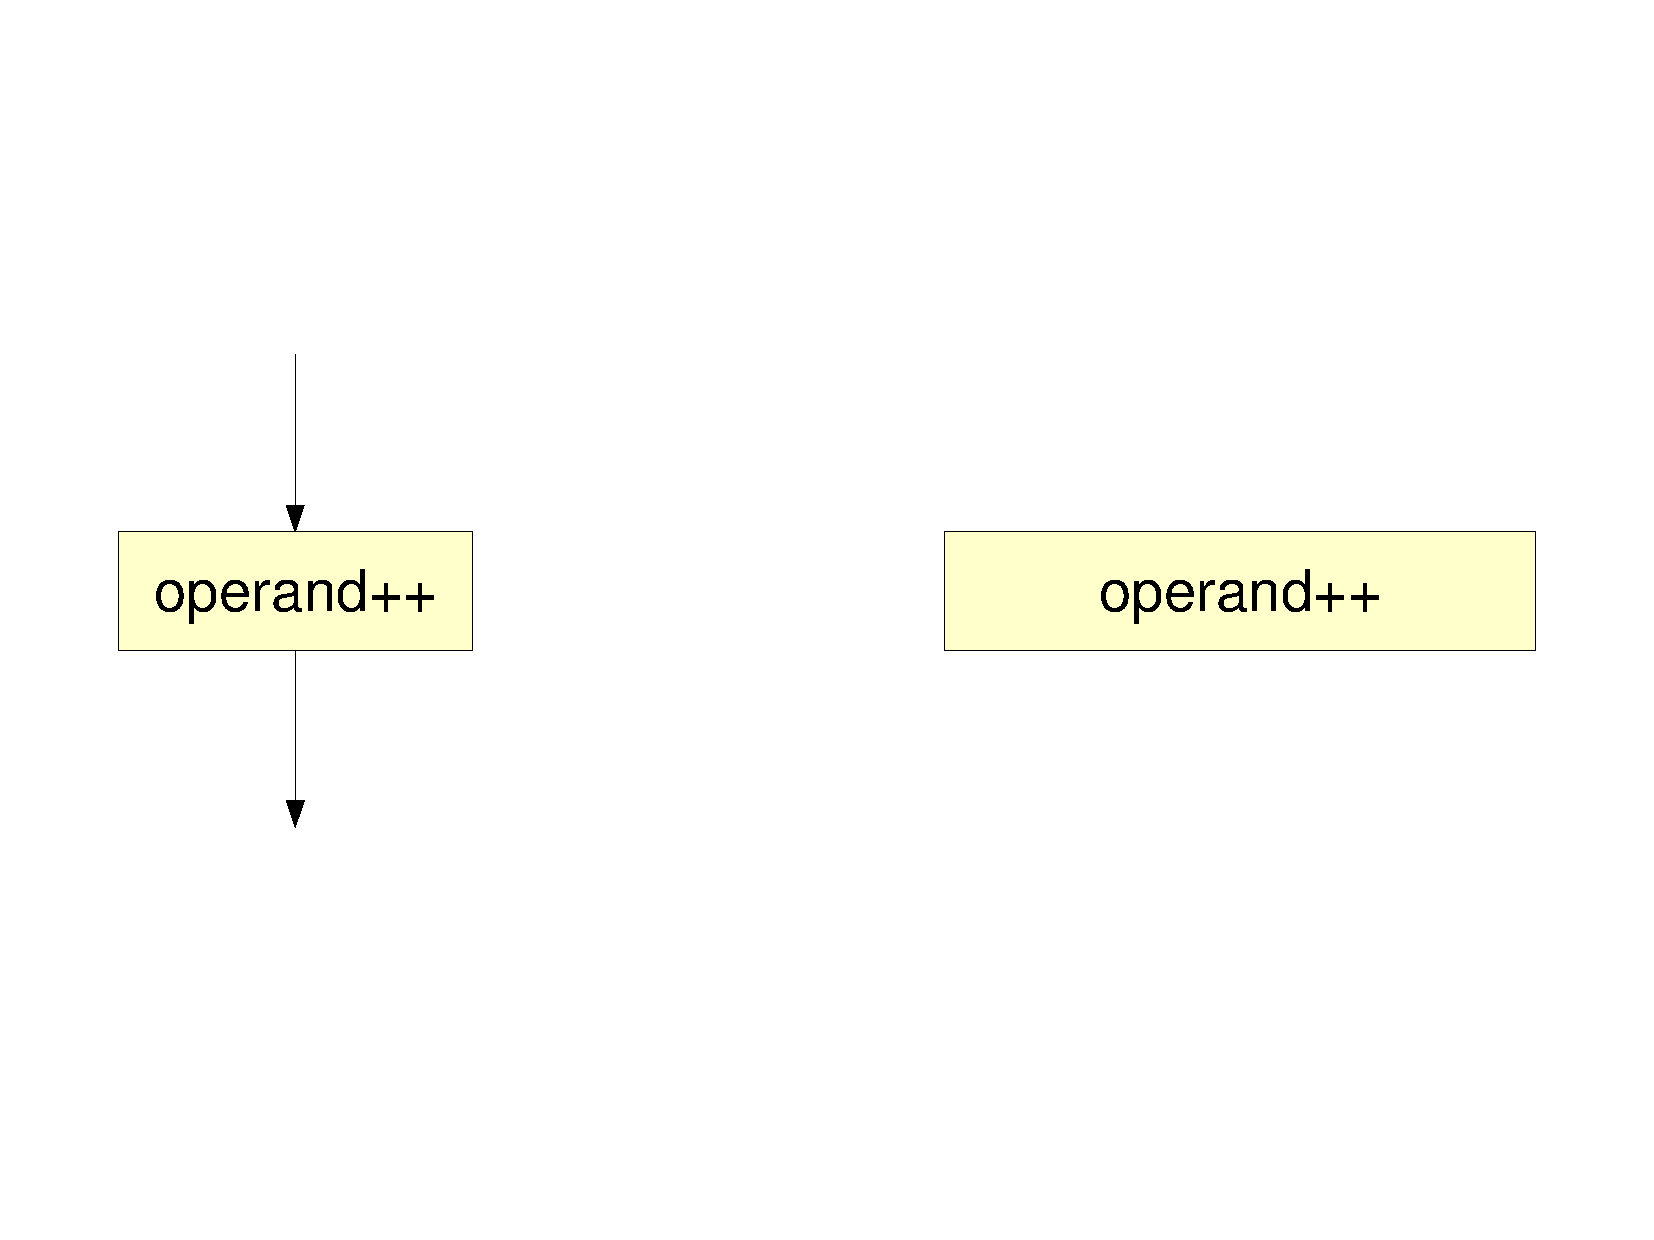
\includegraphics[scale=0.3,angle=-90]{graphic/statement.pdf}
        \caption{Statement as Program Flow Chart and Structure Chart}
        \label{statement_figure}
    \end{center}
\end{figure}

A \emph{Variable} is a placeholder for an abstracted \emph{Data Value}. It
occupies space in memory which is why this space has to be reserved before it
can be used. The reservation is called \emph{Allocation} or \emph{Declaration}
and it states the variable's \emph{Type} and an \emph{Identifier}. Commonly,
variables also get initialised through the \emph{Assignment} of an
\emph{Initial Value}. Here an example for declaration and initialisation
through assignment in \emph{C} code:

\begin{scriptsize}
    \begin{verbatim}
    type identifier = value;
    \end{verbatim}
\end{scriptsize}

Many statements which belong together can form a \emph{Block}, also called
\emph{Compound Statement}. Variables declared in a block are called its
\emph{Local Variables} and loose their validity outside that block. Blocks have
an opening and a closing symbol. Following once more an example in \emph{C}
programming language source code, showing a block with two statements:

\begin{scriptsize}
    \begin{verbatim}
    {
        statement1;
        statement2;
    }
    \end{verbatim}
\end{scriptsize}

%
% $RCSfile: branching.tex,v $
%
% Copyright (C) 2002-2008. Christian Heller.
%
% Permission is granted to copy, distribute and/or modify this document
% under the terms of the GNU Free Documentation License, Version 1.1 or
% any later version published by the Free Software Foundation; with no
% Invariant Sections, with no Front-Cover Texts and with no Back-Cover
% Texts. A copy of the license is included in the section entitled
% "GNU Free Documentation License".
%
% http://www.cybop.net
% - Cybernetics Oriented Programming -
%
% http://www.resmedicinae.org
% - Information in Medicine -
%
% Version: $Revision: 1.1 $ $Date: 2008-08-19 20:41:05 $ $Author: christian $
% Authors: Christian Heller <christian.heller@tuxtax.de>
%

\subsubsection{Branching}
\label{branching_heading}
\index{Branching}
\index{Branch}
\index{Conditional Branching}
\index{Unconditional Branching}
\index{Goto (Jump) Command}
\index{Condition}
\index{Alternative}
\index{Choice}
\index{Multiple Condition}
\index{Switch}
\index{Case}

A block of statements that get only executed at special occasions is called a
\emph{Branch}. Two kinds of branching exist: \emph{Conditional Branching} and
\emph{Unconditional Branching}. An implementation of the latter is the well-known
but also disliked \emph{goto} (\emph{jump}) command. The former depends on a
\emph{Condition}, also called \emph{Alternative} or \emph{Choice} (figure
\ref{condition_figure}), that is its statements are only executed if the
condition's result is true. That way, a condition can change the flow of a
program. A code example follows; it shows conditional branching:

\begin{scriptsize}
    \begin{verbatim}
    if (condition) {
        statements;
    } else {
        statements;
    }
    \end{verbatim}
\end{scriptsize}

\begin{figure}[ht]
    \begin{center}
        \includegraphics[scale=0.3,angle=-90]{graphic/condition.pdf}
        \caption{Condition as Program Flow Chart and Structure Chart}
        \label{condition_figure}
    \end{center}
\end{figure}

Many programming languages offer a \emph{Multiple Condition} control structure
like \emph{switch} or \emph{case}. It is a comfortable possibility to let a
program make a choice out of many alternatives:

\begin{scriptsize}
    \begin{verbatim}
    switch (condition) {
        case constant1:
            statements;
        case constant2:
            statements;
        default:
            statements;
    }
    \end{verbatim}
\end{scriptsize}

Essentially, however, it is a subsumption of a number of simple conditions which
are mostly called \emph{if-else}, and therefore replaceable by such, as shown
following:

\begin{scriptsize}
    \begin{verbatim}
    if (condition == constant1) {
        statements;
    } else if (condition == constant2) {
        statements;
    } else {
        statements;
    }
    \end{verbatim}
\end{scriptsize}

The multiple condition is conceptually no innovation in comparison with the
simple condition and hence pure convenience for the programmer. The interpreter
described in chapter \ref{cybernetics_oriented_interpreter_heading} uses solely
if-then statements.

%
% $RCSfile: looping.tex,v $
%
% Copyright (C) 2002-2008. Christian Heller.
%
% Permission is granted to copy, distribute and/or modify this document
% under the terms of the GNU Free Documentation License, Version 1.1 or
% any later version published by the Free Software Foundation; with no
% Invariant Sections, with no Front-Cover Texts and with no Back-Cover
% Texts. A copy of the license is included in the section entitled
% "GNU Free Documentation License".
%
% http://www.cybop.net
% - Cybernetics Oriented Programming -
%
% http://www.resmedicinae.org
% - Information in Medicine -
%
% Version: $Revision: 1.1 $ $Date: 2008-08-19 20:41:07 $ $Author: christian $
% Authors: Christian Heller <christian.heller@tuxtax.de>
%

\subsubsection{Looping}
\label{looping_heading}
\index{Looping}
\index{Loop Control Structure}
\index{Pre Test Loop}
\index{Post Test Loop}
\index{Counting Loop}
\index{while, while-do}
\index{do-while, repeat-until}
\index{for, for-next}

The \emph{Loop} (figure \ref{loop_figure}) is a control element that allows to
iterate through statements, in other words to execute them repeatedly, several
times. Its concept is quite simple -- a jump backwards in the program. However,
this low-level jump is hidden to the application programmer using a higher-level
SPP language. The loop is indicated by a special keyword instead, for example:

\begin{scriptsize}
    \begin{verbatim}
    while (condition) {
        statements;
    }
    \end{verbatim}
\end{scriptsize}

\begin{figure}[ht]
    \begin{center}
        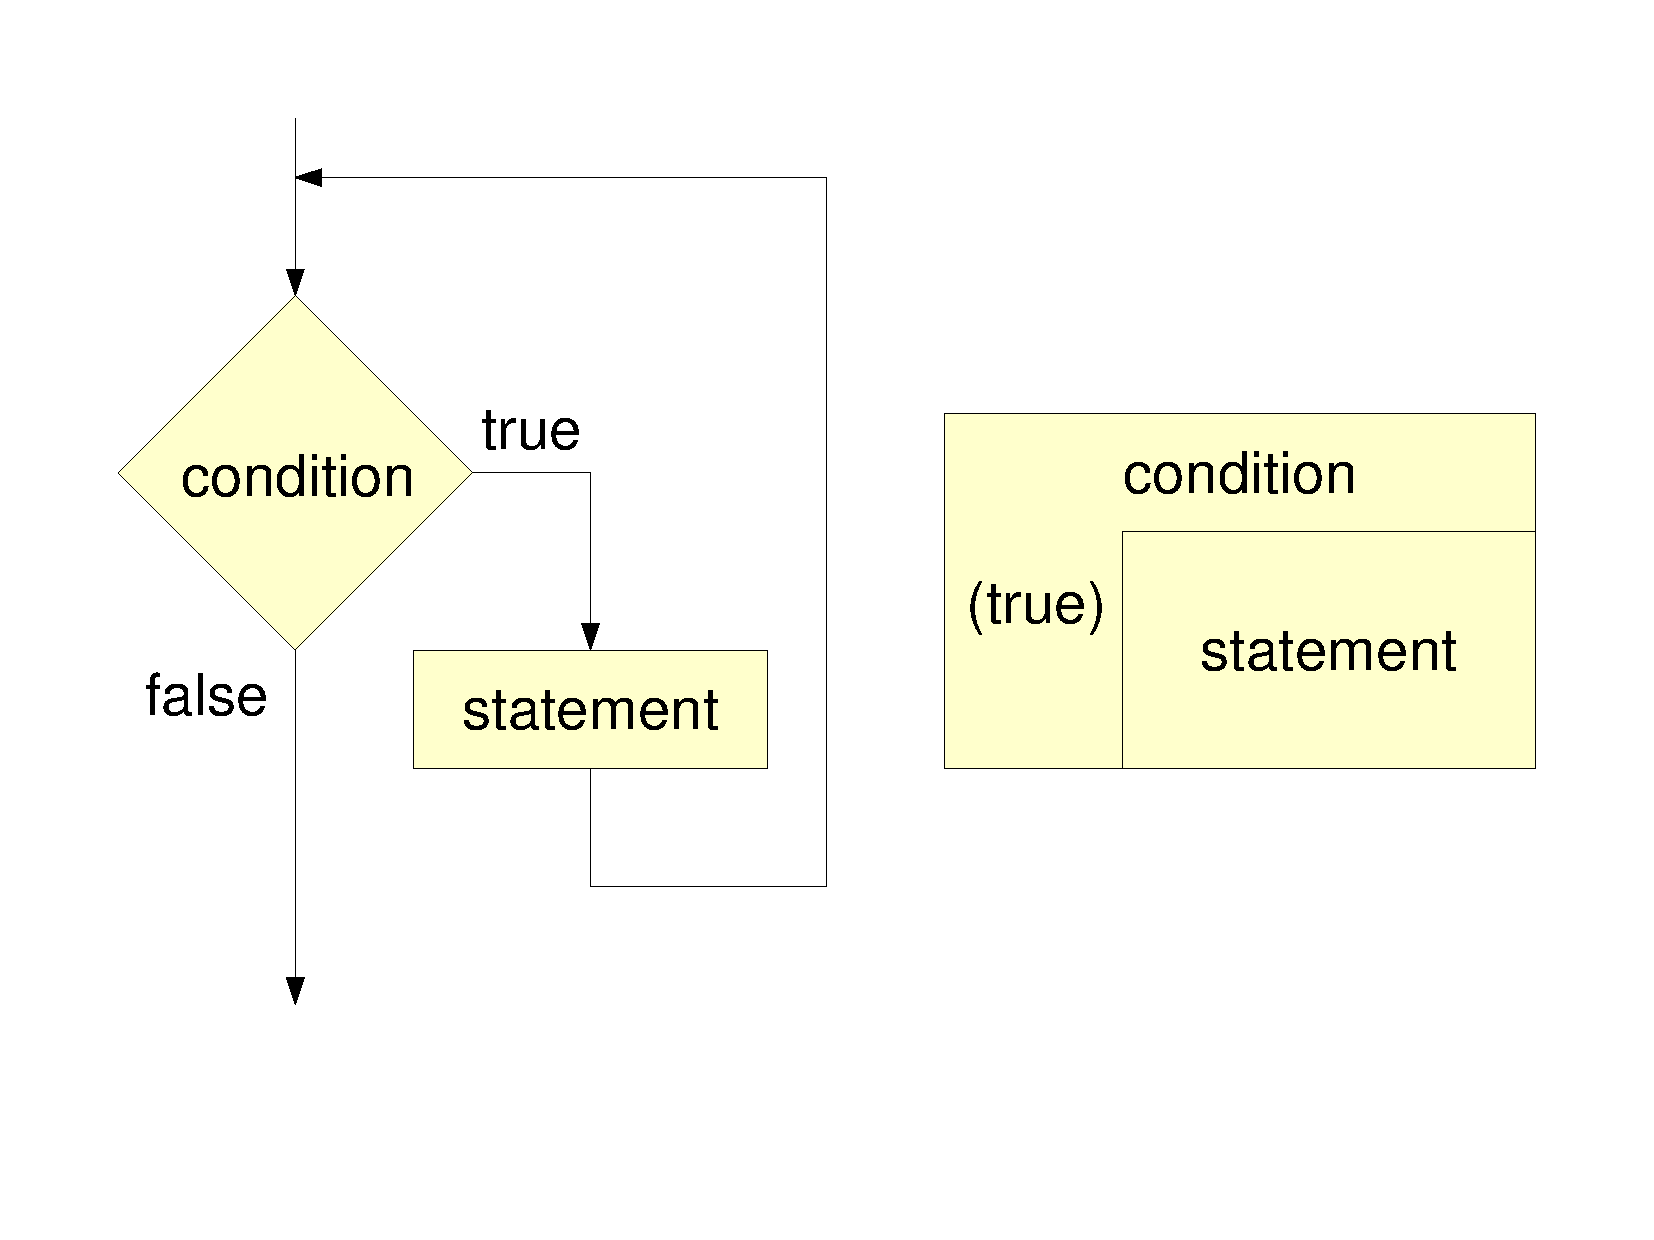
\includegraphics[scale=0.3,angle=-90]{graphic/loop.pdf}
        \caption{Loop as Program Flow Chart and Structure Chart}
        \label{loop_figure}
    \end{center}
\end{figure}

Most programming languages offer three different loop styles, as there are:

\begin{itemize}
    \item[-] Pre-test loop: \emph{while}, \emph{while-do}
    \item[-] Post-test loop: \emph{do-while}, \emph{repeat-until}
    \item[-] Counting Loop: \emph{for}, \emph{for-next}
\end{itemize}

A \emph{Pre-Test Loop} is used when one wants to check a condition before the
statements in the loop body are executed:

\begin{scriptsize}
    \begin{verbatim}
    int i = 0;
    while (i < 1) {
        statements;
        i++;
    }
    \end{verbatim}
\end{scriptsize}

The \emph{Post-Test Loop}, on the other hand, repeats all loop-body statements
until a condition is met:

\begin{scriptsize}
    \begin{verbatim}
    int i = 0;
    do {
        statements;
        i++;
    } while (i < 1);
    \end{verbatim}
\end{scriptsize}

A \emph{Counting Loop}, finally, can be applied when the number of necessary
repetitions of the loop-body statements is known in advance:

\begin{scriptsize}
    \begin{verbatim}
    int i;
    for (i = 0; i < 1; i++) {
        statements;
    }
    \end{verbatim}
\end{scriptsize}

The statements in all three loop examples are only executed once. It is not
difficult to see that the \emph{for} loop can be replaced with a \emph{while}
loop by initialising the \emph{i} variable in its declaration line and moving
the increment statement into the loop's block. But also the \emph{do-while}
loop can be replaced with a \emph{while} loop. If the behaviour does not match
(for example a while block is not executed even once), then changing the initial
loop variable value can solve this problem. Otherwise, modifying the statements
(algorithm) in the block, without changing it logically, will do.

As can be seen: Most variations of the \emph{Looping} concept are just a
convenience for the programmer. They are conceptually identical and can be lead
back to a simple loop with break condition, each. The interpreter described in
chapter \ref{cybernetics_oriented_interpreter_heading} uses just one kind of
loop.


%
% $RCSfile: system_programming.tex,v $
%
% Copyright (C) 2002-2008. Christian Heller.
%
% Permission is granted to copy, distribute and/or modify this document
% under the terms of the GNU Free Documentation License, Version 1.1 or
% any later version published by the Free Software Foundation; with no
% Invariant Sections, with no Front-Cover Texts and with no Back-Cover
% Texts. A copy of the license is included in the section entitled
% "GNU Free Documentation License".
%
% http://www.cybop.net
% - Cybernetics Oriented Programming -
%
% http://www.resmedicinae.org
% - Information in Medicine -
%
% Version: $Revision: 1.1 $ $Date: 2008-08-19 20:41:09 $ $Author: christian $
% Authors: Christian Heller <christian.heller@tuxtax.de>
%

\subsection{System Programming}
\label{system_programming_heading}
\index{System Programming}
\index{System Programming Language}
\index{PL/1}
\index{Pascal}
\index{C}
\index{C++}
\index{Java}
\index{LISP}
\index{Fortran}
\index{Algol}
\index{Assembly Language}
\index{Strong Typing}
\index{Static Typing}
\index{Typing}

After John K. Ousterhout \cite{ousterhout1998}, \emph{System Programming Languages}
such as \emph{PL/1}, \emph{Pascal}, \emph{C} or \emph{C++} or \emph{Java}
(which evolved from higher level languages such as \emph{LISP}, \emph{Fortran} or
\emph{Algol} -- see section \ref{language_history_heading}) had been introduced
as an alternative to \emph{Assembly Languages} and both would differ in two
ways. While in an assembly language, virtually every aspect of a machine were
reflected in the program, each statement representing a single machine
instruction so that programmers had to deal with low-level details such as
register allocation and procedure calling sequences, a system programming
language were:

\begin{enumerate}
    \item \emph{higher level} because its statements did not correspond exactly
        to machine instructions; a compiler would translate each statement in
        the source program into a sequence of binary instructions and handle
        register allocation;
    \item \emph{strongly typed} because programmers needed to declare how each
        piece of information would be used; the language would prevent the
        information from being used in any other way.
\end{enumerate}

Ousterhout uses the term \emph{Typing} to: \textit{refer to the degree to which
the meaning of information is specified in advance of its use}. After him, the
strong typing (also called \emph{Static Typing}) of today's system programming
languages had several advantages, such as:

\begin{itemize}
    \item[-] Better manageability of large programs by differentiating between
        things that must be treated differently
    \item[-] Possible error detection by using type information in compilers
    \item[-] Improved performance by allowing compilers to generate specialized code
\end{itemize}

But there were also a number of disadvantages when using system programming
languages:

\begin{itemize}
    \item[-] Need to declare each variable with a particular type and to use it
        in ways that are appropriate for the type
    \item[-] Difficulty to create new code on the fly due to total segregation
        of data and code
    \item[-] Impossibility to use an object of one type where an object of a
        different type is expected, because variables are collected in objects
        with well-defined substructure and procedures to manipulate them
\end{itemize}

%
% $RCSfile: typeless_programming.tex,v $
%
% Copyright (C) 2002-2008. Christian Heller.
%
% Permission is granted to copy, distribute and/or modify this document
% under the terms of the GNU Free Documentation License, Version 1.1 or
% any later version published by the Free Software Foundation; with no
% Invariant Sections, with no Front-Cover Texts and with no Back-Cover
% Texts. A copy of the license is included in the section entitled
% "GNU Free Documentation License".
%
% http://www.cybop.net
% - Cybernetics Oriented Programming -
%
% http://www.resmedicinae.org
% - Information in Medicine -
%
% Version: $Revision: 1.1 $ $Date: 2008-08-19 20:41:09 $ $Author: christian $
% Authors: Christian Heller <christian.heller@tuxtax.de>
%

\subsection{Typeless Programming}
\label{typeless_programming_heading}
\index{Typeless Programming}
\index{Scripting Language}
\index{Job Control Language}
\index{Batch Language}
\index{Perl}
\index{Python}
\index{Rexx}
\index{Tcl}
\index{Visual Basic}
\index{VB}
\index{Universal Interactive Executive}
\index{UNIX}
\index{Script Oriented Programming}
\index{SOP}
\index{Dynamic Typing}
\index{System Integration Language}
\index{Glue Language}

\emph{Scripting Languages} (formerly also called \emph{Job Control-} or
\emph{Batch Languages} \cite{wikipedia}) such as Perl \cite{wall}, Python
\cite{lutz}, Rexx \cite{ohara}, Tcl \cite{ousterhout1994}, \emph{Visual Basic}
(VB) and the \emph{Universal Interactive Executive} (UNIX) shells overcome the
disadvantages of system programming languages (section
\ref{system_programming_heading}) by being \emph{typeless} and
\emph{interpreted}. The paradigm behind them is sometimes called
\emph{Script Oriented Programming} (SOP).

Ousterhout \cite{ousterhout1998} writes that modern computers were fundamentally
typeless: any word in memory could hold any kind of value, such as an integer, a
floating-point number, a pointer, or an instruction. The meaning of a value were
determined by how it is used: if the program counter pointed at a word of memory
then it were treated as an instruction; if a word were referenced by an integer
\emph{add} instruction then it were treated as an integer; and so on. The same
word could be used in different ways at different times (what is also called
\emph{Dynamic Typing}).

Because scripting languages are intended primarily for plugging together existing
components, they are also referred to as \emph{System Integration Languages} or
\emph{Glue Languages}. They provide a higher level of programming than assembly-
or system programming languages. Through their usage, integrated applications,
after \cite{ousterhout1998}, could be developed five to ten times faster than
with system programming languages. Scripting languages sacrifice execution speed
to improve development speed.

The interpreter described in chapter \ref{cybernetics_oriented_interpreter_heading}
is able to handle data (knowledge) without knowing about their type (kind of
abstraction) in advance, that is at compilation time. Although itself written
in the system programming language \emph{C}, the interpreter is very flexible
when it comes to processing knowledge.

%
% $RCSfile: functional_programming.tex,v $
%
% Copyright (C) 2002-2008. Christian Heller.
%
% Permission is granted to copy, distribute and/or modify this document
% under the terms of the GNU Free Documentation License, Version 1.1 or
% any later version published by the Free Software Foundation; with no
% Invariant Sections, with no Front-Cover Texts and with no Back-Cover
% Texts. A copy of the license is included in the section entitled
% "GNU Free Documentation License".
%
% http://www.cybop.net
% - Cybernetics Oriented Programming -
%
% http://www.resmedicinae.org
% - Information in Medicine -
%
% Version: $Revision: 1.1 $ $Date: 2008-08-19 20:41:06 $ $Author: christian $
% Authors: Christian Heller <christian.heller@tuxtax.de>
%

\subsection{Functional Programming}
\label{functional_programming_heading}
\index{Functional Programming}
\index{Lisp}
\index{Automatic Storage Management}
\index{Integrated Development Environment}
\index{Prolog}
\index{Pascal}
\index{C}
\index{Special Purpose Language}
\index{SPL}
\index{General Purpose Language}
\index{GPL}
\index{Imperative Language}
\index{Functional Language}
\index{Haskell}
\index{Side Effect}
\index{SML}
\index{Scheme}
\index{Association of Lisp Users}

Many languages such as \emph{Lisp} and its relatives cannot be characterised
cleanly as system programming language or scripting language; they are situated
somewhere between. Concepts like \emph{Interpretation} and \emph{Dynamic Typing},
now common in scripting languages, stem from Lisp \cite{ousterhout1998}. Others like
\emph{Automatic Storage Management} and \emph{Integrated Development Environments},
now used in both scripting- and system programming languages, were introduced by
Lisp as well. Peter Norvig writes in \cite{norvig}:

\begin{quote}
    There is a myth that Lisp (and Prolog) are \emph{Special Purpose Languages}
    (SPL), while languages such as Pascal and C are \emph{General Purpose} (GPL).
    Actually, just the reverse is true. Pascal and C are special-purpose languages
    for manipulating the registers and memory of a \emph{von Neumann}-style computer.
    The majority of their syntax is devoted to arithmetic and Boolean expressions,
    and while they provide some facilities for forming data structures, they have
    poor mechanisms for procedural abstraction or control abstraction. In addition,
    they are designed for the \emph{state-oriented} style of programming: computing
    a result by changing the value of variables through assignment statements.
\end{quote}

The \emph{Frequently Asked Questions} (FAQ) edited by Graham Hutton \cite{hutton}
distinguish between \emph{Imperative Languages} and \emph{Functional Languages}.
System programming languages as introduced in previous sections belong to the
first group. To calculate the sum of the integers from 1 to 10, for example,
they would probably use a simple loop and repeatedly update the values held in
an accumulator variable \emph{total} and a counter variable \emph{i}:

\begin{scriptsize}
    \begin{verbatim}
    int total = 0;
    for (int i = 1; i <= 10; ++i) {
        total += i;
    }
    \end{verbatim}
\end{scriptsize}

A functional language like \emph{Haskell} would express the same program
\emph{without} any variable updates, by evaluating an expression, as shown
below. Variable updates, that is \textit{computational effects caused by
expression evaluation that persist after the evaluation is completed}
\cite{hutton} are called \emph{Side Effects}.

\begin{scriptsize}
    \begin{verbatim}
    sum [1..10]
    \end{verbatim}
\end{scriptsize}

The following two examples \cite{hutton} show the same program in two other
functional languages, namely \emph{SML} and \emph{Scheme}:

\begin{scriptsize}
    \begin{verbatim}
    let fun sum i tot = if i = 0 then tot else sum (i - 1) (tot + i)
    in sum 10 0
    end
    \end{verbatim}
\end{scriptsize}

\begin{scriptsize}
    \begin{verbatim}
    (define sum
    (lambda (from total)
        (if (= 0 from)
            total
            (sum (- from 1) (+ total from)))))
    (sum 10 0)
    \end{verbatim}
\end{scriptsize}

The \emph{Association of Lisp Users} \cite{commonlisp} points out the absence
of side effects and explains \emph{Functional Programming} as follows:

\begin{quote}
    Functional programming describes all computer operations as mathematical
    functions on inputs. Typically, a function can be created and returned from
    other functions as first-class data. This function object may then be passed
    as input to other functions, perhaps be composed with other functions, and
    eventually, applied to inputs to produce a value. Objects can be defined in
    terms of functions that encapsulate certain data, and operations on objects
    can be defined by functions encapsulating the objects. Purely functional
    languages do not have assignment, as all side-effecting can be defined in
    terms of functions that encapsulate the changed data. Procedural languages
    essentially perform everything as side-effects to data structures. A purely
    procedural language would have no functions, but might have subroutines of
    no arguments that returned no values, and performed certain assignments and
    other operations based on the data it found stored in the system.
\end{quote}

The interpreter described in chapter \ref{cybernetics_oriented_interpreter_heading}
manipulates \emph{all} data (knowledge) as if it would be one huge side effect.
Data (knowledge models) are not bundled with-, but kept completely outside any
functions/ procedures. Only references to these data are handed over as
parameters.

%
% $RCSfile: logical_programming.tex,v $
%
% Copyright (C) 2002-2008. Christian Heller.
%
% Permission is granted to copy, distribute and/or modify this document
% under the terms of the GNU Free Documentation License, Version 1.1 or
% any later version published by the Free Software Foundation; with no
% Invariant Sections, with no Front-Cover Texts and with no Back-Cover
% Texts. A copy of the license is included in the section entitled
% "GNU Free Documentation License".
%
% http://www.cybop.net
% - Cybernetics Oriented Programming -
%
% http://www.resmedicinae.org
% - Information in Medicine -
%
% Version: $Revision: 1.1 $ $Date: 2008-08-19 20:41:07 $ $Author: christian $
% Authors: Christian Heller <christian.heller@tuxtax.de>
%

\subsection{Logical Programming}
\label{logical_programming_heading}
\index{Logical Programming}
\index{Declarative Programming}
\index{Artificial Intelligence}
\index{AI}
\index{Expert System}
\index{Automated Theorem Proving}
\index{Monkey and Banana Problem}
\index{Prolog}
\index{Mercury}
\index{TyRuBa}

\emph{Functional Programming} as introduced in the previous section is one kind
of \emph{Declarative Programming}, which describes to the computer a set of
conditions and lets the computer figure out how to satisfy them \cite{wikipedia}.
Another kind is \emph{Logical Programming}. It specifies a set of attributes
that a solution should have -- rather than a set of steps to obtain such a
solution. Schematically, the logical programming process follows the equation:

\begin{scriptsize}
    \begin{verbatim}
    facts + rules = results
    \end{verbatim}
\end{scriptsize}

Logical programming was strongly influenced by \emph{Artificial Intelligence}
(AI) and is applied in domains such as \emph{Expert Systems}, where the program
generates a recommendation or answer from a large model of the application
domain, and \emph{Automated Theorem Proving}, where the program generates novel
theorems to extend some existing body of theory. \cite{wikipedia}

The \emph{Monkey and Banana Problem} is a famous example studied in the community
of logical programming \cite{wikipedia}: \textit{Instead of the programmer
explicitly specifying the path for the monkey to reach the banana, the computer
actually reasons out a possible way that the monkey reaches the banana.}

A prominent logical language representative is \emph{Prolog}; a more recent one
is \emph{Mercury}; an \emph{Open Source Software} (OSS) one is \emph{TyRuBa}.

%
% $RCSfile: data_manipulation_language.tex,v $
%
% Copyright (C) 2002-2008. Christian Heller.
%
% Permission is granted to copy, distribute and/or modify this document
% under the terms of the GNU Free Documentation License, Version 1.1 or
% any later version published by the Free Software Foundation; with no
% Invariant Sections, with no Front-Cover Texts and with no Back-Cover
% Texts. A copy of the license is included in the section entitled
% "GNU Free Documentation License".
%
% http://www.cybop.net
% - Cybernetics Oriented Programming -
%
% http://www.resmedicinae.org
% - Information in Medicine -
%
% Version: $Revision: 1.1 $ $Date: 2008-08-19 20:41:06 $ $Author: christian $
% Authors: Christian Heller <christian.heller@tuxtax.de>
%

\subsection{Data Manipulation Language}
\label{data_manipulation_language_heading}
\index{Data Manipulation Language}
\index{DML}
\index{Structured Query Language}
\index{SQL}
\index{Structured English Query Language}
\index{SEQUEL}
\index{Relational Database Management System}
\index{RDBMS}
\index{Data Definition Language}
\index{DDL}
\index{Data Control Language}
\index{DCL}

A \emph{Data Manipulation Language} (DML), after \cite{wikipedia}, is:
\textit{a family of computer languages used by computer programs or database
users to retrieve, insert, delete and update data in a database}. As most
popular DML, the source mentions the \emph{Structured Query Language} (SQL)
that was originally developed as \emph{Structured English Query Language}
(SEQUEL) by \emph{International Business Machines} (IBM), after the model
described by Edgar F. Codd in \cite{codd}.

Technically, SQL is a set-based, declarative computer language that, after
\cite{wikipedia}, could be used to create, modify and retrieve data from
\emph{Relational Database Management Systems} (RDBMS). Its keywords are often
shared into the three groups:

\begin{itemize}
    \item[-] \emph{Data Manipulation Language} (DML): SELECT, INSERT, UPDATE, DELETE
    \item[-] \emph{Data Definition Language} (DDL): CREATE, DROP
    \item[-] \emph{Data Control Language} (DCL): GRANT, REVOKE
\end{itemize}

Since the details of that language are outside the scope of this work, they are
not elaborated further here, but can be learned at for example \cite{sqltutorial}.
%The \emph{Entity Relationship Model} (ERM) as basic data model behind
%\emph{Relational Database Management Systems} (RDBMS) (section
%\ref{database_server_heading}), however, is described briefly in section
%\ref{entity_relationship_model_heading}.

%
% $RCSfile: markup_language.tex,v $
%
% Copyright (C) 2002-2008. Christian Heller.
%
% Permission is granted to copy, distribute and/or modify this document
% under the terms of the GNU Free Documentation License, Version 1.1 or
% any later version published by the Free Software Foundation; with no
% Invariant Sections, with no Front-Cover Texts and with no Back-Cover
% Texts. A copy of the license is included in the section entitled
% "GNU Free Documentation License".
%
% http://www.cybop.net
% - Cybernetics Oriented Programming -
%
% http://www.resmedicinae.org
% - Information in Medicine -
%
% Version: $Revision: 1.1 $ $Date: 2008-08-19 20:41:07 $ $Author: christian $
% Authors: Christian Heller <christian.heller@tuxtax.de>
%

\subsection{Markup Language}
\label{markup_language_heading}
\index{Markup Language}
\index{World Wide Web}
\index{WWW}
\index{Style of a Document}
\index{Structure of a Document}
\index{Content of a Document}
\index{TeX}
\index{Lamport TeX}
\index{LaTeX}
\index{LaTeXe}
\index{Scribe}
\index{Standard Generalized Markup Language}
\index{SGML}
\index{Extensible Markup Language}
\index{XML}
\index{Hypertext Markup Language}
\index{HTML}
\index{DocBook}
\index{Text Encoding Initiative}
\index{TEI}

At latest with the distribution of the \emph{World Wide Web} (WWW),
\emph{Markup Languages} increasingly gained in popularity. A markup language
separates the presentation \emph{Style} of a document from its logical
\emph{Structure} and \emph{Content}. Well-known representatives of markup
languages, two famous of which being described in the following sections, are
\cite{wikipedia}:

\begin{itemize}
    \item[-] \emph{\TeX} / \emph{Lamport \TeX} (\LaTeX, \LaTeXe)
    \item[-] \emph{Scribe}
    \item[-] \emph{Standard Generalized Markup Language} (SGML)
    \item[-] \emph{Extensible Markup Language} (XML)
    \item[-] \emph{Hypertext Markup Language} (HTML)
    \item[-] \emph{DocBook}
    \item[-] \emph{Text Encoding Initiative} (TEI)
\end{itemize}

Recently, more and more projects appear that try to use markup languages not
just for document markup, but also for declarative programming.% More on this in
%section \ref{xml_based_programming_heading}.
Before coming to the actual markup languages, the paradigm of
\emph{Literate Programming} and its idea to use markup tokens for distinguishing
source code and documentation, is investigated.

%
% $RCSfile: literate_programming.tex,v $
%
% Copyright (C) 2002-2008. Christian Heller.
%
% Permission is granted to copy, distribute and/or modify this document
% under the terms of the GNU Free Documentation License, Version 1.1 or
% any later version published by the Free Software Foundation; with no
% Invariant Sections, with no Front-Cover Texts and with no Back-Cover
% Texts. A copy of the license is included in the section entitled
% "GNU Free Documentation License".
%
% http://www.cybop.net
% - Cybernetics Oriented Programming -
%
% http://www.resmedicinae.org
% - Information in Medicine -
%
% Version: $Revision: 1.1 $ $Date: 2008-08-19 20:41:07 $ $Author: christian $
% Authors: Christian Heller <christian.heller@tuxtax.de>
%

\subsubsection{Literate Programming}
\label{literate_programming_heading}
\index{Literate Programming}
\index{Token Character}
\index{Commercial At @}
\index{Re-ordering of Code}
\index{Typeset Code and Documentation}
\index{Cross Referencing}
\index{Source Code Documentation}
\index{JavaDoc}
\index{Doxygen}
\index{DOC++}

Ross Williams writes in \cite[section 1.1]{williams}:

\begin{quote}
    A traditional computer program consists of a text file containing program
    code. Scattered in amongst the program code are comments which describe the
    various parts of the code. In \emph{Literate Programming}, the emphasis is
    reversed. Instead of writing code containing documentation, the literate
    programmer writes documentation containing code.
\end{quote}

In other words, \emph{Literate Programming} pays more attention to proper source
code documentation than classical programming languages do. It mostly offers
special \emph{Token} characters like the \emph{Commercial At} character \emph{@}
for example, which serve as code delimiters. The delimited blocks are determined
by particular tools such as a preprocessor that filters out program code to be
processed further. All source information together (input document, commentaries,
program code) is used to generate typeset documentation files in one or more
formats.

Williams \cite{williams} means that the literate programming system provided
far more than: \textit{just a reversal of the priority of comments and code.}
In its full-blown form, a good literate programming facility could provide:

\begin{itemize}
    \item[-] \emph{Re-ordering of Code:} Some programming languages force the
        programmer to give the various program parts in a particular order.
    \item[-] \emph{Typeset Code and Documentation:} Because a literate programming
        utility sees all the code, it can use its knowledge of the programming
        language and the features of the typesetting language to typeset the
        program code as if it were appearing in a technical journal.
    \item[-] \emph{Cross referencing:} Because a literate tool sees all the code
        and documentation, it is able to generate extensive cross referencing
        information in the typeset documentation, which makes the printed program
        document more easy to navigate and partially compensates for the lack of
        an automatic searching facility when reading printed documentation.
\end{itemize}

It is true, the actual instructions and algorithms in between commentaries are
written in (or translated into) a system programming- or other kind of language.
But literate programming places its focus on source code \emph{Documentation}
for which it uses \emph{Markup} tokens, which is why it was classified under
\emph{Markup Language} in this work.

Although literate programming itself has not gained that much popularity, its
idea of using markup tokens to generate more expressive source code documentation
has. Several up-to-date programming environments make use of it. A well-known
example is the \emph{JavaDoc} tool \cite{javadoc}; other systems are
\emph{Doxygen} \cite{doxygen} or \emph{DOC++} \cite{docpp}.

%
% $RCSfile: tex_and_latex.tex,v $
%
% Copyright (C) 2002-2008. Christian Heller.
%
% Permission is granted to copy, distribute and/or modify this document
% under the terms of the GNU Free Documentation License, Version 1.1 or
% any later version published by the Free Software Foundation; with no
% Invariant Sections, with no Front-Cover Texts and with no Back-Cover
% Texts. A copy of the license is included in the section entitled
% "GNU Free Documentation License".
%
% http://www.cybop.net
% - Cybernetics Oriented Programming -
%
% http://www.resmedicinae.org
% - Information in Medicine -
%
% Version: $Revision: 1.1 $ $Date: 2008-08-19 20:41:09 $ $Author: christian $
% Authors: Christian Heller <christian.heller@tuxtax.de>
%

\subsubsection{TeX and LaTeX}
\label{tex_and_latex_heading}
\index{Tex}
\index{Lamport TeX}
\index{LaTeX}
\index{LaTeXe}
\index{Device Independent Format}
\index{DVI}
\index{PDFTeX}
\index{Portable Document Format}
\index{PDF}
\index{TeX User Group}
\index{TUG}
\index{Desktop Publishing}
\index{DTP}

The special-purpose \TeX\ \cite{tex} language is the centre-piece of a
typesetting system which, due to its well-formatted output of complex
mathematical formulas and generally high-quality typesetting, is especially
popular among academic circles of mathematicians, physicists and computer
scientists \cite{latextutorial}. The Wikipedia encyclopedia \cite{wikipedia}
writes:

\begin{quote}
    \TeX\ is a macro and token based language: many commands, including most
    user-defined ones, are expanded on the fly until only unexpandable tokens
    remain which get executed. Expansion itself is practically side-effect free.
    Tail recursion of macros takes no memory, and if-then-else constructs are
    available. \ldots

    The \TeX\ system has precise knowledge of the sizes of all characters and
    symbols, and using this information, it computes the optimal arrangement of
    letters per line and lines per page. It then produces a \emph{Device Independent}
    (DVI) file containing the final locations of all characters. The DVI file
    can be printed directly given an appropriate printer driver, or it can be
    converted to other formats.
\end{quote}

The \emph{PDFTeX} translator program is often used to bypass all DVI generation,
by creating \emph{Portable Document Format} (PDF) files directly.

Nowadays, \TeX\ is mostly used with a template extension called \emph{Lamport \TeX}
(\LaTeX, \LaTeXe) \cite{latex}. The Indian \emph{\TeX\ Users Group} (TUG) writes
\cite{latextutorial}: \textit{\LaTeX\ is a document preparation system which
adds a set of functions that make the \TeX\ language friendlier than using
the primitives provided by it.} It offers programmable \emph{Desktop Publishing}
(DTP) features and extensive facilities for automating most aspects of
typesetting. \cite{wikipedia}

The most important feature of \TeX\ for this work is its kind of relating meta-
with structural information. Two examples may help here:

\begin{scriptsize}
    \begin{verbatim}
    \documentclass[a4paper,12pt]{book}
    \includegraphics[scale=0.3]{path/file.pdf}
    \end{verbatim}
\end{scriptsize}

The first statement determines \emph{book} as document class for a document to
be written. It contains additional information such as paper- and font size, in
square brackets. The second statement refers to a graphics file to be included.
The additional information given in square brackets here is the scale factor.
With a different syntax, but in a comparable manner, the knowledge modelling
language introduced in chapter \ref{cybernetics_oriented_language_heading} does
relate structural- with meta information.

%
% $RCSfile: extensible_markup_language.tex,v $
%
% Copyright (C) 2002-2008. Christian Heller.
%
% Permission is granted to copy, distribute and/or modify this document
% under the terms of the GNU Free Documentation License, Version 1.1 or
% any later version published by the Free Software Foundation; with no
% Invariant Sections, with no Front-Cover Texts and with no Back-Cover
% Texts. A copy of the license is included in the section entitled
% "GNU Free Documentation License".
%
% http://www.cybop.net
% - Cybernetics Oriented Programming -
%
% http://www.resmedicinae.org
% - Information in Medicine -
%
% Version: $Revision: 1.1 $ $Date: 2008-08-19 20:41:06 $ $Author: christian $
% Authors: Christian Heller <christian.heller@tuxtax.de>
%

\subsubsection{Extensible Markup Language}
\label{extensible_markup_language_heading}
\index{Extensible Markup Language}
\index{XML}
\index{World Wide Web}
\index{WWW}
\index{World Wide Web Consortium}
\index{W3C}
\index{Standard Generalized Markup Language}
\index{SGML}
\index{Hypertext Markup Language}
\index{HTML}
\index{Document Publishing}
\index{Data Transfer}
\index{GUI Design}
\index{Workflow Composition}
\index{Database Storage}
\index{Domain Modelling}

A popular, very flexible, yet simple language playing an increasingly important
role in the exchange of a wide variety of data on the \emph{World Wide Web}
(WWW) and elsewhere is the \emph{Extensible Markup Language} (XML) \cite{xml},
defined by the \emph{World Wide Web Consortium} (W3C) \cite{w3c}. Being a text
format derived as simplified subset (dialect) of the
\emph{Standard Generalized Markup Language} (SGML) \cite{sgml}, it allows to
structure and store information hierarchically as \emph{Document} file. Norman
Walsh \cite{walsh} writes:

\begin{quote}
    A markup language is a mechanism to \emph{identify structures} in a document.
    The XML specification defines a standard way to \emph{add markup} to documents.
\end{quote}

And the XML Cover Pages \cite{sgmlmetamarkup} state:

\begin{quote}
    Both SGML and XML are \emph{meta} languages because they are used for
    defining \emph{markup} languages. A markup language defined using SGML or
    XML has a specific vocabulary (labels for elements and attributes) and a
    declared syntax (grammar defining the hierarchy and other features).
\end{quote}

Historically, markup languages became widely known through the
\emph{Hypertext Markup Language} (HTML) as language of the Web. To overcome its
limitations, XML was originally \emph{designed to meet the challenges of large-
scale electronic publishing} \cite{xml}. Today, XML is applied in many different
areas, for example:

\begin{itemize}
    \item[-] Document Publishing \cite{docbook}
    \item[-] Data Transfer \cite{soap}
    \item[-] GUI Design \cite{xul, uiml, ecml, xaml}
    \item[-] Workflow Composition \cite{oio, intershop}
    \item[-] Database Storage \cite{exist, dbxml}
    \item[-] Domain Modelling \cite{xmlschema, damloil}
\end{itemize}

Yet in the opinion of Robin Cover \cite{xmlsemantics}, the usability of XML for
domain modelling is limited. He writes:

\begin{quote}
    Just like its parent metalanguage (SGML), XML has no formal mechanism to
    support the declaration of semantic integrity constraints, and XML processors
    have no means of validating object semantics even if these are declared
    informally in an XML DTD. XML processors will have no inherent understanding
    of document object semantics because XML (meta-)markup languages have no
    predefined application-level processing semantics. XML thus formally governs
    syntax only -- not semantics.

    In fact, XML syntax is designed for representing an encoded serialization,
    and thus has a very limited range of expression for modeling complex object
    semantics, where \emph{Semantics} fundamentally means an intricate web of
    constrained relationships and properties. Otherwise stated: XML is a poor
    language for data modelling \ldots
\end{quote}

The XML-based language described in chapter \ref{cybernetics_oriented_language_heading}
proves the opposite. By applying a common knowledge modelling schema (chapter
\ref{knowledge_schema_heading}), it allows to model arbitrary meta information
(complex object semantics). Robin Cover continues \cite{xmlsemantics}:

\begin{quote}
    The notion of \emph{Attribute} might have been more useful except that XML
    supports only a flat data model for the value of an attribute in a
    name-value pair (essentially \emph{String}). This flat model cannot easily
    capture complex attribute notions such as would be predicated of abstracted
    real world objects, where attribute values are themselves typically
    represented by complex objects, either owned or referenced.
\end{quote}

This criticism of Cover is absolutely correct. It can be circumvented, though.
The language introduced in chapter \ref{cybernetics_oriented_language_heading}
permits one attribute to store a (file) path to an external compound knowledge
template and is thus capable of representing compound properties (complex
attribute notions). One problem remains, however: When serialising compound
knowledge models consisting of other compound models, the quotation mark as
attribute value delimiter is not sufficient, because the beginning and end of
an attribute value may get mixed up. Solving it, the XML standard needs to be
injured (chapter \ref{cybernetics_oriented_language_heading}).


%
% $RCSfile: page_description_language.tex,v $
%
% Copyright (C) 2002-2008. Christian Heller.
%
% Permission is granted to copy, distribute and/or modify this document
% under the terms of the GNU Free Documentation License, Version 1.1 or
% any later version published by the Free Software Foundation; with no
% Invariant Sections, with no Front-Cover Texts and with no Back-Cover
% Texts. A copy of the license is included in the section entitled
% "GNU Free Documentation License".
%
% http://www.cybop.net
% - Cybernetics Oriented Programming -
%
% http://www.resmedicinae.org
% - Information in Medicine -
%
% Version: $Revision: 1.1 $ $Date: 2008-08-19 20:41:08 $ $Author: christian $
% Authors: Christian Heller <christian.heller@tuxtax.de>
%

\subsection{Page Description Language}
\label{page_description_language_heading}
\index{Page Description Language}
\index{PDL}
\index{Device Independent Format}
\index{DVI}
\index{Printer Control Language}
\index{PCL}
\index{PostScript}
\index{PS}
\index{Portable Document Format}
\index{PDF}

In order to be (more or less) complete in the language overview given in this
work, the \emph{Page Description Language} (PDL) as further category shall be
mentioned here as well. It describes the contents and appearance (text,
graphical shapes, images) of a page to be printed in a device-independent,
higher-level way than an actual output bitmap \cite{wikipedia}. It may
therefore serve as an: \textit{interchange standard for (the) transmission and
storage of printable documents} \cite{foldoc}. Well-known PDL representatives
are:

\begin{itemize}
    \item[-] \emph{Device Independent} (DVI) format
    \item[-] \emph{Printer Control Language} (PCL)
    \item[-] \emph{PostScript} (PS)
    \item[-] \emph{Portable Document Format} (PDF)
\end{itemize}

After \cite{foldoc}, \emph{PostScript} is a: \textit{full programming language,
rather than a series of low-level escape sequences}. It is stack-based and
interpreted. These properties made it the: \textit{language of choice for
graphical output, until PDF appeared}. The following PostScript code example
\cite{wikipedia} computes (3 + 4) * (5 - 1):

\begin{scriptsize}
    \begin{verbatim}
    3 4 add 5 1 sub mul
    \end{verbatim}
\end{scriptsize}

%
% $RCSfile: hardware_description_language.tex,v $
%
% Copyright (C) 2002-2008. Christian Heller.
%
% Permission is granted to copy, distribute and/or modify this document
% under the terms of the GNU Free Documentation License, Version 1.1 or
% any later version published by the Free Software Foundation; with no
% Invariant Sections, with no Front-Cover Texts and with no Back-Cover
% Texts. A copy of the license is included in the section entitled
% "GNU Free Documentation License".
%
% http://www.cybop.net
% - Cybernetics Oriented Programming -
%
% http://www.resmedicinae.org
% - Information in Medicine -
%
% Version: $Revision: 1.1 $ $Date: 2008-08-19 20:41:07 $ $Author: christian $
% Authors: Christian Heller <christian.heller@tuxtax.de>
%

\subsection{Hardware Description Language}
\label{hardware_description_language_heading}
\index{Hardware Description Language}
\index{HDL}
\index{Electronic Circuit}
\index{Application Specific Integrated Circuit}
\index{ASIC}
\index{Field Programmable Gate Array}
\index{FPGA}
\index{Very High Speed Integrated Circuit}
\index{VHSIC}
\index{VHDL}
\index{Verilog HDL}
\index{SystemC}
\index{Electronic Data Interchange Format}
\index{EDIF}
\index{Joint Electron Device Engineering Council}
\index{JEDEC}
\index{Programmable Logic Device}
\index{PLD}

\emph{Hardware Description Language} (HDL) is an umbrella term for any computer
language formally describing \emph{Electronic Circuits}, that is their design and
operation, as well as tests to verify their operation by means of \emph{Simulation}
\cite{wikipedia}. HDLs used for the design of digital circuits like
\emph{Application Specific Integrated Circuits} (ASIC) or
\emph{Field Programmable Gate Arrays} (FPGA) include:

\begin{itemize}
    \item[-] \emph{Very High Speed Integrated Circuit} (VHSIC) HDL (VHDL) \cite[standard 1164]{ieee}
    \item[-] \emph{Verilog HDL} \cite[standard 1364-2001]{ieee}
    \item[-] \emph{SystemC} \cite{doulos}
\end{itemize}

Although being similar, HDLs are not programming languages. \textit{HDL's syntax
and semantics include explicit notations for expressing time and concurrency which
are the primary attributes of hardware}, as \cite{wikipedia} writes and adds:

\begin{quote}
    An HDL compiler often works in several stages, first producing a logic
    description file in a proprietary format, then converting that to a logic
    description file in the industry-standard
    \emph{Electronic Data Interchange Format} (EDIF), then converting that to a
    \emph{Joint Electron Device Engineering Council} (JEDEC) format file. The
    JEDEC file contains instructions to a \emph{Programmable Logic Device} (PLD)
    programmer for building logic. On the other hand, a software (programming
    language) compiler generates instructions to a microprocessor for moving data.
\end{quote}

The following sections of this chapter will be about programming-, not hardware
description concepts.

%
% $RCSfile: object_oriented_programming.tex,v $
%
% Copyright (C) 2002-2008. Christian Heller.
%
% Permission is granted to copy, distribute and/or modify this document
% under the terms of the GNU Free Documentation License, Version 1.1 or
% any later version published by the Free Software Foundation; with no
% Invariant Sections, with no Front-Cover Texts and with no Back-Cover
% Texts. A copy of the license is included in the section entitled
% "GNU Free Documentation License".
%
% http://www.cybop.net
% - Cybernetics Oriented Programming -
%
% http://www.resmedicinae.org
% - Information in Medicine -
%
% Version: $Revision: 1.1 $ $Date: 2008-08-19 20:41:07 $ $Author: christian $
% Authors: Christian Heller <christian.heller@tuxtax.de>
%

\subsection{Object Oriented Programming}
\label{object_oriented_programming_heading}
\index{Object Oriented Programming}
\index{OOP}
\index{Structured and Procedural Programming}
\index{SPP}
\index{Object Orientation}
\index{OO}
\index{Smalltalk}
\index{C++}
\index{C}
\index{Python}
\index{Common Lisp Object System}
\index{CLOS}
\index{Common Lisp}
\index{CL}
\index{Lisp}
\index{Class}
\index{Java}
\index{Unified Modeling Language}
\index{UML}
\index{UML Tool}

With the emerge of \emph{Object Oriented} (OO) languages, an additional
programming paradigm got introduced. That is, many principles such as
\emph{Structured and Procedural Programming} (SPP) were still holding true but
got extended through \emph{Object Oriented Programming} (OOP). Examples of OOP
languages, often defined by simply extending an existing language, are:

\begin{itemize}
    \item[-] \emph{Smalltalk} \cite{smalltalk}
    \item[-] \emph{C++}, extending the \emph{C} system programming language
        (section \ref{system_programming_heading})
    \item[-] \emph{Python}, as typeless programming language
        (section \ref{typeless_programming_heading})
    \item[-] \emph{Common Lisp Object System} (CLOS), extending the
        \emph{Common Lisp} (CL)\\dialect of the \emph{Lisp} functional
        programming language (section \ref{functional_programming_heading})
\end{itemize}

The following sections describe the main concepts behind OOP in brief. Although
many of them represent improvements to SPP, this work will point out their
weaknesses, too. The merger of attributes (data) and methods (operations) into
one common data structure called \emph{Class}, for example, will be criticised
and eliminated later in this work (chapter \ref{state_and_logic_heading}).

Code examples in the \emph{Java} programming language are given as well as
\emph{Unified Modeling Language} (UML) diagrams. The UML is a semi-formal,
graphical description language that offers elements for the concepts of
\emph{Object Orientation} (OO). To some extend, programs can be designed,
generated and documented using special applications called \emph{UML Tools}.

%
% $RCSfile: classification.tex,v $
%
% Copyright (C) 2002-2008. Christian Heller.
%
% Permission is granted to copy, distribute and/or modify this document
% under the terms of the GNU Free Documentation License, Version 1.1 or
% any later version published by the Free Software Foundation; with no
% Invariant Sections, with no Front-Cover Texts and with no Back-Cover
% Texts. A copy of the license is included in the section entitled
% "GNU Free Documentation License".
%
% http://www.cybop.net
% - Cybernetics Oriented Programming -
%
% http://www.resmedicinae.org
% - Information in Medicine -
%
% Version: $Revision: 1.1 $ $Date: 2008-08-19 20:41:05 $ $Author: christian $
% Authors: Christian Heller <christian.heller@tuxtax.de>
%

\subsubsection{Classification}
\label{classification_heading}
\index{Classification}
\index{Class}
\index{Attribute}
\index{Method}
\index{Structured Data Type}
\index{Struct}
\index{Record}
\index{Structured and Procedural Programming}
\index{SPP}
\index{Java}
\index{Global Variable}
\index{Instance}
\index{Object}
\index{Instantiation}
\index{Abstract Class}
\index{Interface}
\index{Inner Class}
\index{Bundling of Attributes and Methods}

The main idea of object oriented programming is to structure program code into
\emph{Classes} owning \emph{Attributes} and \emph{Methods} (figure
\ref{classification_figure}). They are comparable to the structured data types
(\emph{struct}, \emph{record}) of \emph{Structured and Procedural Programming}
(SPP) (section \ref{structured_and_procedural_programming_heading}) that can
own fields representing properties, but not behaviour. A class definition in
\emph{Java} source code looks like this:

\begin{scriptsize}
    \begin{verbatim}
    public class Example {
        private Type attribute;
        public void method(Type parameter) {
        }
    }
    \end{verbatim}
\end{scriptsize}

\begin{figure}[ht]
    \begin{center}
        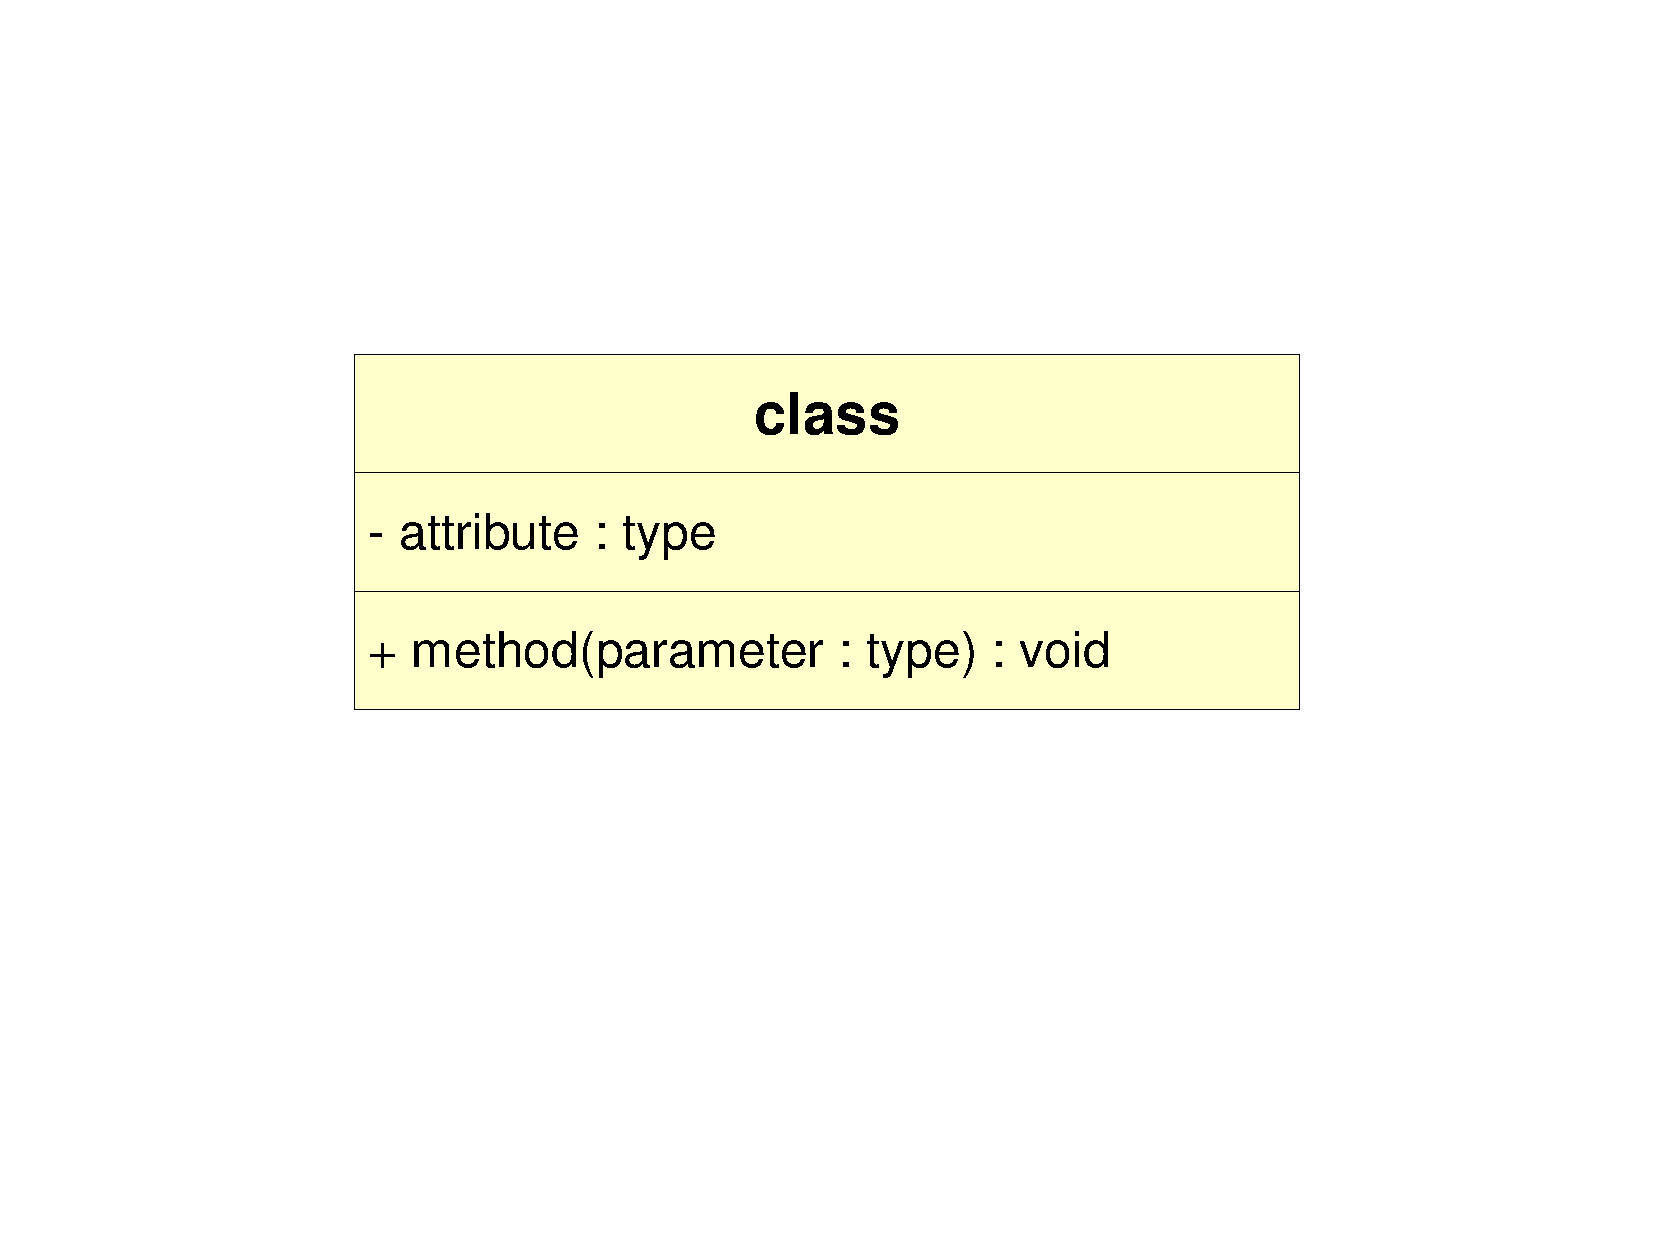
\includegraphics[scale=0.3,angle=-90]{graphic/classification.pdf}
        \caption{Classification as UML Diagram}
        \label{classification_figure}
    \end{center}
\end{figure}

While procedures and many variables in SPP are global, that is only exist once,
classes are treated as types of which many \emph{Instances} (also called
\emph{Objects}) can be created, including attributes and methods. In OOP, such
memory allocation is called \emph{Instantiation}.

Two related data types are \emph{Abstract Class} and \emph{Interface}. An
abstract class can hold attributes and (partly abstract) methods. Just like
interfaces, abstract classes cannot be instantiated. An interface is yet more
restricted in that it can only have constants but not attributes and only
declarations but not actual implementations of methods. Interfaces are commonly
used to \cite{steppan}:

\begin{itemize}
    \item[-] Realise multiple inheritance (section \ref{inheritance_heading})
    \item[-] Encapsulate components (section \ref{interface_and_implementation_heading})
    \item[-] Pool common methods (section \ref{separation_of_concerns_heading})
\end{itemize}

Specialities like \emph{Inner Classes} \cite{java} with limited scope of
validity are of minor importance to the argumentation of this document and not
further explained here.

The \emph{Bundling} of attributes and methods (state and logic) causes more
system interdependencies and complications than were predictable. It is a big
disadvantage that affects all modern object-oriented systems. \cite{heller2004}
Certainly, the bundling stems from best intentions to receive cleaner code by
keeping not only attributes but also methods in a common module, such avoiding
\emph{wild} and \emph{global} procedures. But now, modules not only have to
refer to other modules for accessing their state data; the same is needed for
accessing their logic in form of method calls.

With OOP, the number of cross-relations between modules, and inter-dependencies
between system layers may rise dramatically. In reality, state- and logic
properties are two \emph{different} things that have to be kept in different
places! Both can have a similar, hierarchical structure but each is a concept on
its own, as chapter \ref{state_and_logic_heading} will show.

%
% $RCSfile: encapsulation.tex,v $
%
% Copyright (C) 2002-2008. Christian Heller.
%
% Permission is granted to copy, distribute and/or modify this document
% under the terms of the GNU Free Documentation License, Version 1.1 or
% any later version published by the Free Software Foundation; with no
% Invariant Sections, with no Front-Cover Texts and with no Back-Cover
% Texts. A copy of the license is included in the section entitled
% "GNU Free Documentation License".
%
% http://www.cybop.net
% - Cybernetics Oriented Programming -
%
% http://www.resmedicinae.org
% - Information in Medicine -
%
% Version: $Revision: 1.1 $ $Date: 2008-08-19 20:41:06 $ $Author: christian $
% Authors: Christian Heller <christian.heller@tuxtax.de>
%

\subsubsection{Encapsulation}
\label{encapsulation_heading}
\index{Encapsulation}
\index{Access Method}
\index{Java}
\index{Information Hiding}
\index{Data Hiding}
\index{public}
\index{protected}
\index{private}
\index{Delphi}
\index{published}

One recommendation of object oriented programming is that the properties of an
object created as instance of a class be protected through special
\emph{Access Methods} (figure \ref{encapsulation_figure}). A \emph{Java} code
example can be found below. The intention is not to expose class attributes to
other classes by minimising direct access to them and such to provide some
security by preventing illegal access to an object's interna. Therefore, this
paradigm is called \emph{Encapsulation} or \emph{Information-/ Data Hiding}.
Another advantage is that if an attribute changes its name, then only one place
in the code (the access method), instead of hundreds, needs to be updated.

\begin{scriptsize}
    \begin{verbatim}
    public class example_class {
        private Type attribute;
        public void set_attribute(Type a) {
            this.attribute = a;
        }
        public Type get_attribute() {
            return this.attribute;
        }
    }
    \end{verbatim}
\end{scriptsize}

\begin{figure}[ht]
    \begin{center}
        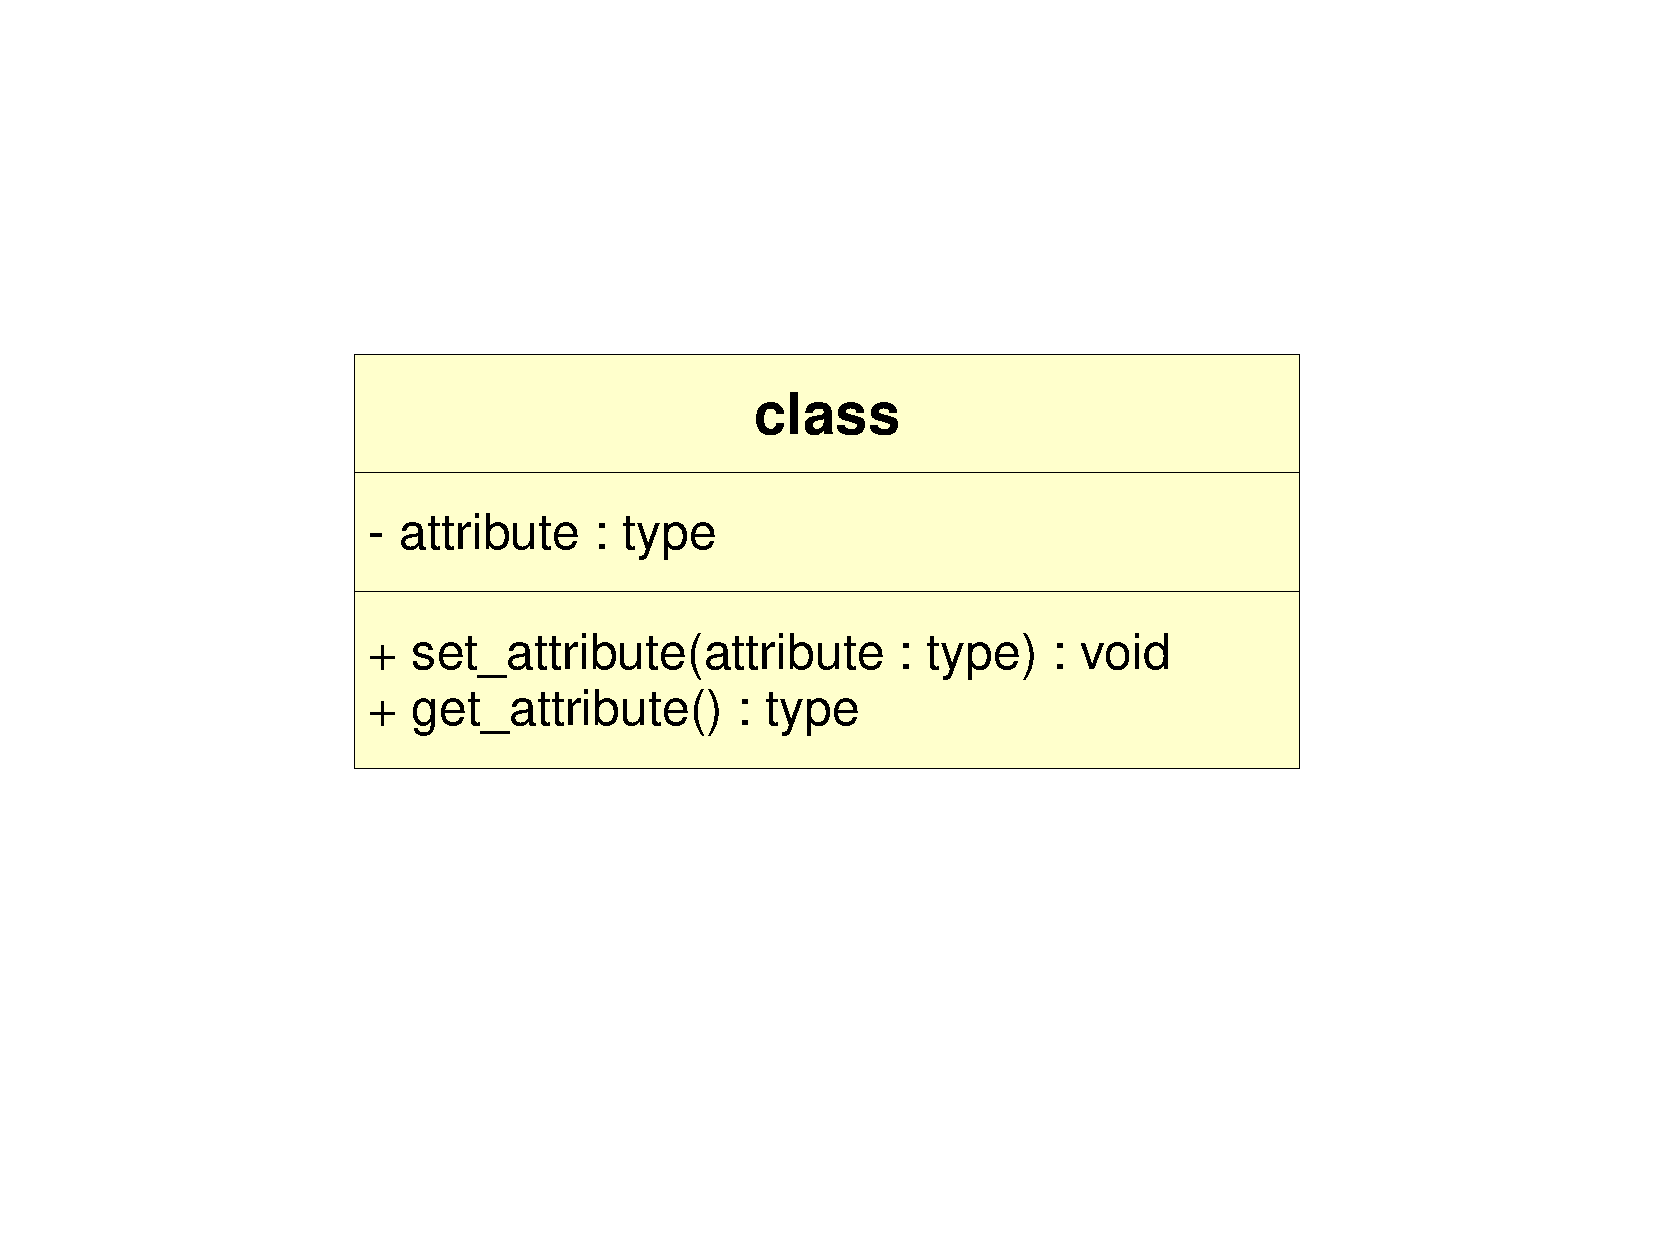
\includegraphics[scale=0.3,angle=-90]{graphic/encapsulation.pdf}
        \caption{Encapsulation as UML Diagram}
        \label{encapsulation_figure}
    \end{center}
\end{figure}

Special keywords are necessary to ensure proper encapsulation by making
attributes and methods \emph{visible} to only certain outside objects. These
keywords are: \emph{public}, \emph{protected} and \emph{private}. In the
\emph{Java} programming language \cite{java}, an additional package protection
level is applied when none of the aforementioned keywords is found. The
\emph{Delphi} language \cite{warken} knows an additional \emph{published}
keyword that makes properties visible in its object-inspector tool. Other
languages may contain further variations of access limitations.

The recommendation to encapsulate attributes produces thousands of lines of
source code whose usefulness is at least questionnable \cite{hellerbohl}. In
about 90\% of cases (practical experience of the author of this document), the
\emph{set} and \emph{get} methods consist of only one single line accessing an
attribute value which in the end is the same as accessing that attribute
directly. Sometimes, additional lines with a trigger function to update other
parts of the system are added. They get invoked whenever an attribute value of
the called object is changed by a \emph{set} method:

\begin{scriptsize}
    \begin{verbatim}
    public void set_attribute(Type a) {
        this.attribute = a;
        get_update_manager().update(this);
    }
    \end{verbatim}
\end{scriptsize}

But, as shown below, this update notification could as well be taken over by
the object that was calling the \emph{set} method:

\begin{scriptsize}
    \begin{verbatim}
    public void method() {
        example_object.set_attribute(a);
        get_update_manager().update(example_object);
    }
    \end{verbatim}
\end{scriptsize}

The argumentation that \textit{in this case a lot of redundant code would be
produced since the update function has to be implemented in every calling
object, instead of just once in the called object} does not really hold true
when looking into programming practice. The number of external objects calling
an object is mostly very well manageable. It finally seems that thousands of
\emph{set}/ \emph{get} access methods could be eliminated which would lead to a
tremendous code reduction and improved clearity.

The language introduced in chapter \ref{cybernetics_oriented_language_heading}
does not use encapsulation and the attributes (state knowledge) and methods
(logic knowledge) modelled in it are not bundled together.

%
% $RCSfile: inheritance.tex,v $
%
% Copyright (C) 2002-2008. Christian Heller.
%
% Permission is granted to copy, distribute and/or modify this document
% under the terms of the GNU Free Documentation License, Version 1.1 or
% any later version published by the Free Software Foundation; with no
% Invariant Sections, with no Front-Cover Texts and with no Back-Cover
% Texts. A copy of the license is included in the section entitled
% "GNU Free Documentation License".
%
% http://www.cybop.net
% - Cybernetics Oriented Programming -
%
% http://www.resmedicinae.org
% - Information in Medicine -
%
% Version: $Revision: 1.1 $ $Date: 2008-08-19 20:41:07 $ $Author: christian $
% Authors: Christian Heller <christian.heller@tuxtax.de>
%

\subsubsection{Inheritance}
\label{inheritance_heading}
\index{Inheritance}
\index{Superior Class}
\index{Parent Class}
\index{C++}
\index{Multiple Inheritance}
\index{Java}
\index{Single Inheritance}
\index{Interface}
\index{Application Programming Interface}
\index{API}

\emph{Inheritance} allows for code minimisation by letting classes inherit
attributes and methods from their \emph{superior} (sometimes called \emph{parent})
class (figure \ref{inheritance_figure}). Redundant code can such be avoided and
existing code can be reused. An inheriting class in \emph{Java} source code
looks like this:

\begin{scriptsize}
    \begin{verbatim}
    public class example extends super_class {
    }
    \end{verbatim}
\end{scriptsize}

\begin{figure}[ht]
    \begin{center}
        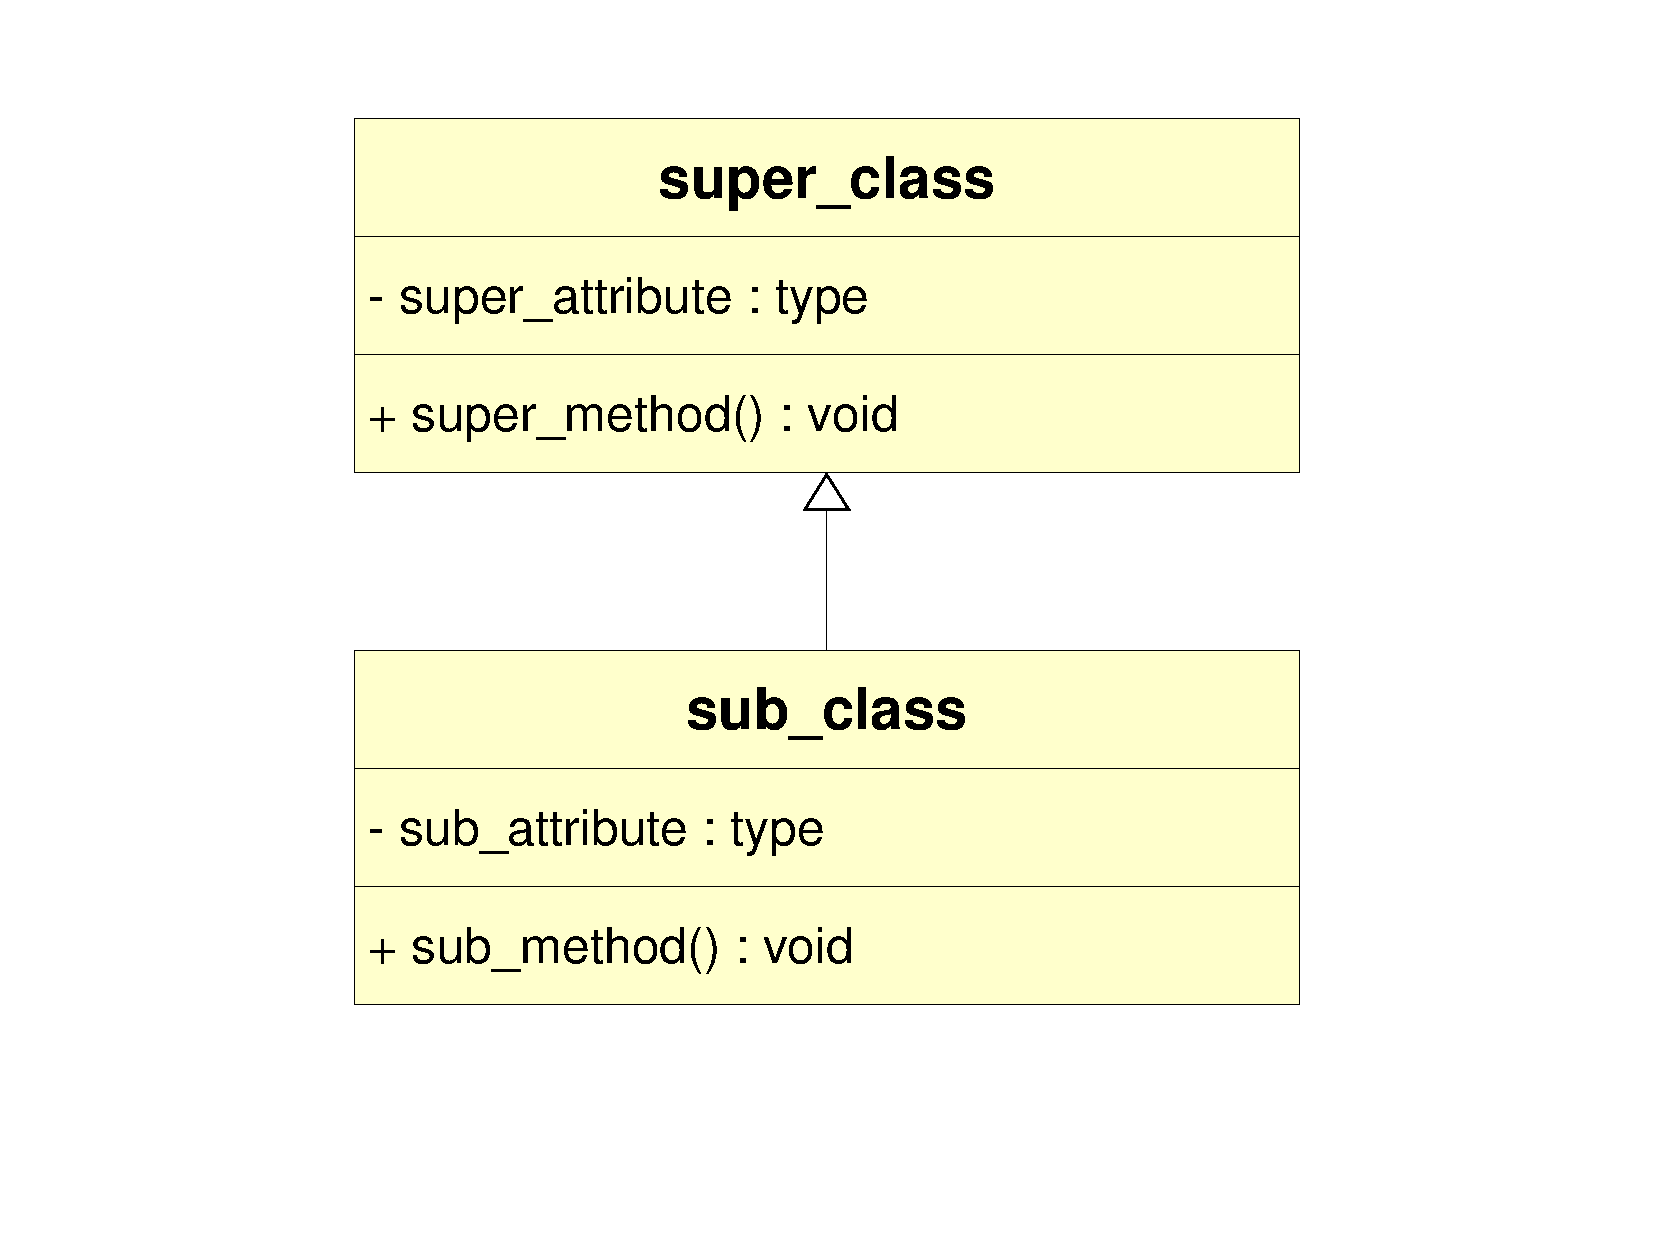
\includegraphics[scale=0.3,angle=-90]{graphic/inheritance.pdf}
        \caption{Inheritance as UML Diagram}
        \label{inheritance_figure}
    \end{center}
\end{figure}

Some object oriented programming languages (such as \emph{C++}) permit
\emph{Multiple Inheritance}. Classes written in those languages can have more
than one superior class. Other languages (such as \emph{Java}) that have
\emph{Single Inheritance} only, sometimes offer to \emph{inherit}
(\emph{realise}/ \emph{implement}) multiple interfaces. An interface forces its
subclasses to implement all methods it declares (more on this in section
\ref{interface_and_implementation_heading}) and can such provide a common
\emph{Application Programming Interface} (API) which makes classes
interchangeable and hence encourages reuse.

%
% $RCSfile: fragile_base_class.tex,v $
%
% Copyright (C) 2002-2008. Christian Heller.
%
% Permission is granted to copy, distribute and/or modify this document
% under the terms of the GNU Free Documentation License, Version 1.1 or
% any later version published by the Free Software Foundation; with no
% Invariant Sections, with no Front-Cover Texts and with no Back-Cover
% Texts. A copy of the license is included in the section entitled
% "GNU Free Documentation License".
%
% http://www.cybop.net
% - Cybernetics Oriented Programming -
%
% http://www.resmedicinae.org
% - Information in Medicine -
%
% Version: $Revision: 1.1 $ $Date: 2008-08-19 20:41:06 $ $Author: christian $
% Authors: Christian Heller <christian.heller@tuxtax.de>
%

\subsubsection{Fragile Base Class}
\label{fragile_base_class_heading}
\index{Fragile Base Class (Problem)}
\index{Implementation Inheritance}
\index{Subclass}
\index{Superclass}
\index{Class Hierarchy}
\index{Cascade of Change}
\index{Reusability}
\index{Flexibility}
\index{Cyclic Method Dependencies}
\index{Self-calling Assumptions of a Class Method}
\index{Base Class Access}
\index{Modifier Invariant Function}

Despite the possible code reduction through class inheritance, there are some
negative effects that hinder just this code reduction and reuse. John K.
Ousterhout writes in his article \cite{ousterhout1998}:

\begin{quote}
    Implementation inheritance, where one class borrows code that was written
    for another class, is a bad idea that makes software harder to manage and
    reuse. It binds the implementations of classes together so that neither
    class can be understood without the other: a subclass cannot be understood
    without knowing how the inherited methods are implemented in its superclass,
    and a superclass cannot be understood without knowing how its methods are
    inherited in subclasses. In a complex class hierarchy, no individual class
    can be understood without understanding all the other classes in the
    hierarchy. Even worse, a class cannot be separated from its hierarchy for
    reuse. Multiple inheritance makes these problems even worse. Implementation
    inheritance causes the same intertwining and brittleness that have been
    observed when goto statements are overused. As a result, object-oriented
    systems often suffer from complexity and lack of reuse.
\end{quote}

Unwanted dependencies caused simply by the usage of inheritance are called
\emph{Fragile Base Class Problem} \cite[section \emph{Layers}; p. 48]{buschmann}.
The source code changes resulting from base class manipulation are also called
\emph{Cascade of Change} \cite[Vorwort]{gruhn}. They are just the opposite of
what inheritance was actually intended to be for: \emph{Reusability}. Leonid
Mikhajlov and Emil Sekerinski \cite{mikhajlov} write:

\begin{quote}
    This problem occurs in open object-oriented systems employing code
    inheritance as an implementation reuse mechanism. System developers unaware
    of extensions to the system developed by its users may produce a seemingly
    acceptable revision of a base class which may damage its extensions.
    The fragile base class problem becomes apparent during maintenance of open
    object-oriented systems, but requires consideration during design.
\end{quote}

They identify the following \emph{Restrictions} \cite{mikhajlov} disciplining the
code inheritance mechanism, thus avoiding the \emph{Fragile Base Class Problem},
but on the cost of general \emph{Flexibility}:

\begin{itemize}
    \item[-] \emph{No cycles:} A base class revision and a modifier should not
        jointly introduce new cyclic method dependencies.
    \item[-] \emph{No revision self-calling assumptions:} Revision class methods
        should not make any additional assumptions about the behaviour of the
        other methods of itself. Only the behaviour described in the base class
        may be taken into consideration.
    \item[-] \emph{No base class down-calling assumptions:} Methods of a modifier
        should disregard the fact that base class self-calls can get redirected
        to the modifier itself. In this case bodies of the corresponding methods
        in the base class should be considered instead, as if there were no
        dynamic binding.
    \item[-] \emph{No direct access to base class state:} An extension class
        may not access the state of its base class directly, but only through
        calling base class methods.
    \item[-] \emph{No modifier invariant function:} A modifier should not bind
        values of its instance variables with values of the intended base class
        instance variables to generate an invariant.
\end{itemize}

In order to remain highly flexible and to avoid the fragile base class problem,
the language described in chapter \ref{cybernetics_oriented_language_heading}
does not use inheritance, although it could be extended to do so. In this case,
of course, its interpreter (chapter \ref{cybernetics_oriented_interpreter_heading})
would have to be adapted as well.

%
% $RCSfile: polymorphism.tex,v $
%
% Copyright (C) 2002-2008. Christian Heller.
%
% Permission is granted to copy, distribute and/or modify this document
% under the terms of the GNU Free Documentation License, Version 1.1 or
% any later version published by the Free Software Foundation; with no
% Invariant Sections, with no Front-Cover Texts and with no Back-Cover
% Texts. A copy of the license is included in the section entitled
% "GNU Free Documentation License".
%
% http://www.cybop.net
% - Cybernetics Oriented Programming -
%
% http://www.resmedicinae.org
% - Information in Medicine -
%
% Version: $Revision: 1.1 $ $Date: 2008-08-19 20:41:08 $ $Author: christian $
% Authors: Christian Heller <christian.heller@tuxtax.de>
%

\subsubsection{Polymorphism}
\label{polymorphism_heading}
\index{Polymorphism}
\index{Method Overloading}
\index{Method Overriding}
\index{Super Class}
\index{Sub Class}
\index{super}

Another object oriented feature that comes with inheritance is
\emph{Polymorphism}. It allows methods to be \emph{overloaded} (sometimes
called \emph{overridden}). That is, on two objects created from different
classes inheriting from each other, the right equally named method will be
called by the language interpreter program (figure \ref{polymorphism_figure}),
which leads to different behaviour depending on the current object context.
Following is a \emph{Java} code example overloading a method to gain
polymorphic behaviour:

\begin{scriptsize}
    \begin{verbatim}
    public class super_class {
        public void method() {
            do_something();
        }
    }
    public class sub_class extends super_class {
        public void method() {
            do_something_else();
        }
    }
    \end{verbatim}
\end{scriptsize}

\begin{figure}[ht]
    \begin{center}
        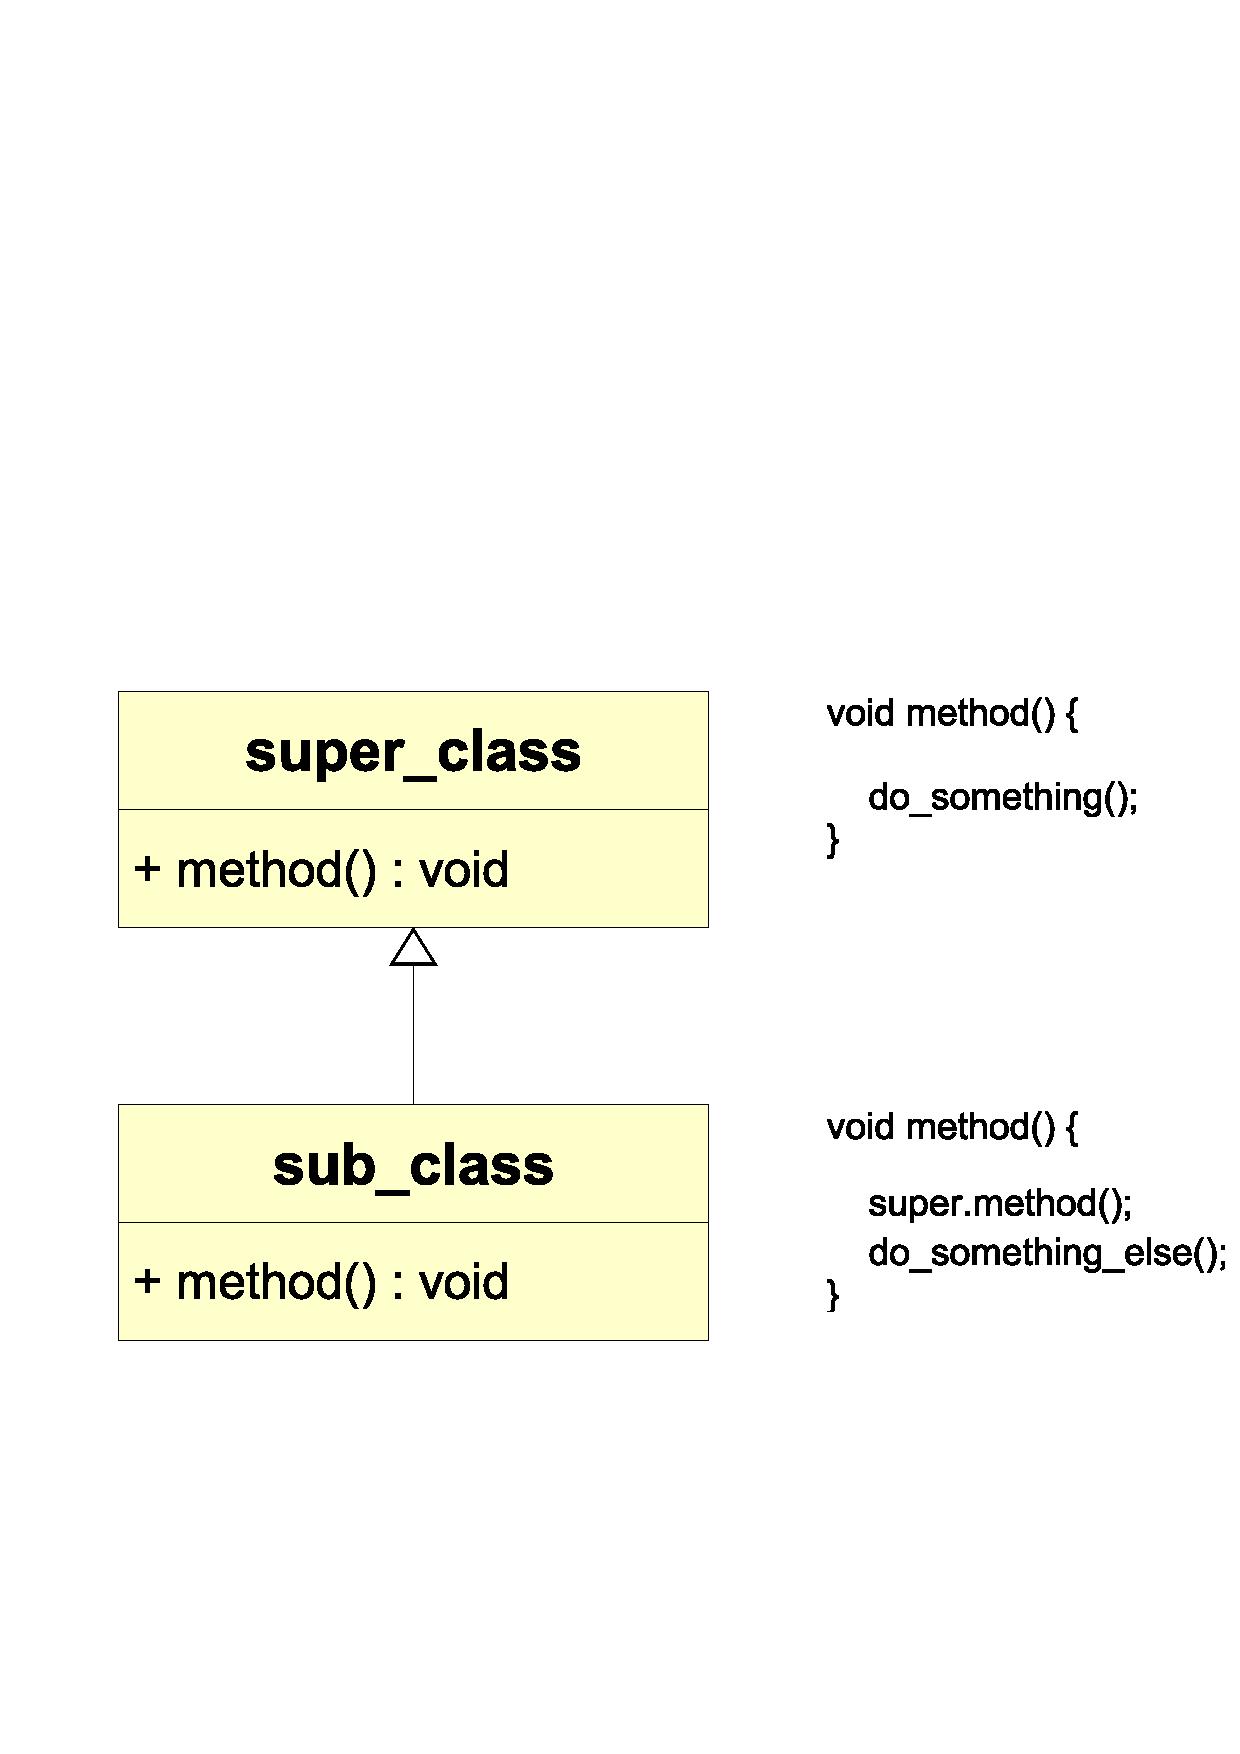
\includegraphics[scale=0.3,angle=-90]{graphic/polymorphism.pdf}
        \caption{Polymorphism as UML Diagram}
        \label{polymorphism_figure}
    \end{center}
\end{figure}

If objects instantiated from a sub class want to make use of the functionality
contained in the super class' equally named method, the sub class' method needs
to call the super class' method explicitly using the keyword \emph{super}:

\begin{scriptsize}
    \begin{verbatim}
    public class sub_class extends super_class {
        public void method() {
            super.method();
            do_something_else();
        }
    }
    \end{verbatim}
\end{scriptsize}

%
% $RCSfile: container.tex,v $
%
% Copyright (C) 2002-2008. Christian Heller.
%
% Permission is granted to copy, distribute and/or modify this document
% under the terms of the GNU Free Documentation License, Version 1.1 or
% any later version published by the Free Software Foundation; with no
% Invariant Sections, with no Front-Cover Texts and with no Back-Cover
% Texts. A copy of the license is included in the section entitled
% "GNU Free Documentation License".
%
% http://www.cybop.net
% - Cybernetics Oriented Programming -
%
% http://www.resmedicinae.org
% - Information in Medicine -
%
% Version: $Revision: 1.1 $ $Date: 2008-08-19 20:41:06 $ $Author: christian $
% Authors: Christian Heller <christian.heller@tuxtax.de>
%

\subsubsection{Container}
\label{container_heading}
\index{Container}
\index{Primitive Type}
\index{Java Container Framework}
\index{Collection}
\index{Map}
\index{Tree}
\index{Standard Template Library}
\index{STL}
\index{Sequence}
\index{Associative Container}

An object that got created through instantiating a class represents an
allocated area in a computer's memory which needs to be referenced in order to
be able to work with it, and to finally destroy it. The size of that area may
change \emph{dynamically}, depending on how the properties of the object are
manipulated. Primitive types like \emph{integer} or \emph{double} also reserve
memory space, only that the size of that space is \emph{not} dynamic; it is
pre-defined by the programming language, for each type. All
\emph{Structured- and Procedural Programming} (SPP) languages and some
\emph{Object Oriented Programming} (OOP) languages, like Java, offer standard
primitive types.

\begin{figure}[ht]
    \begin{center}
        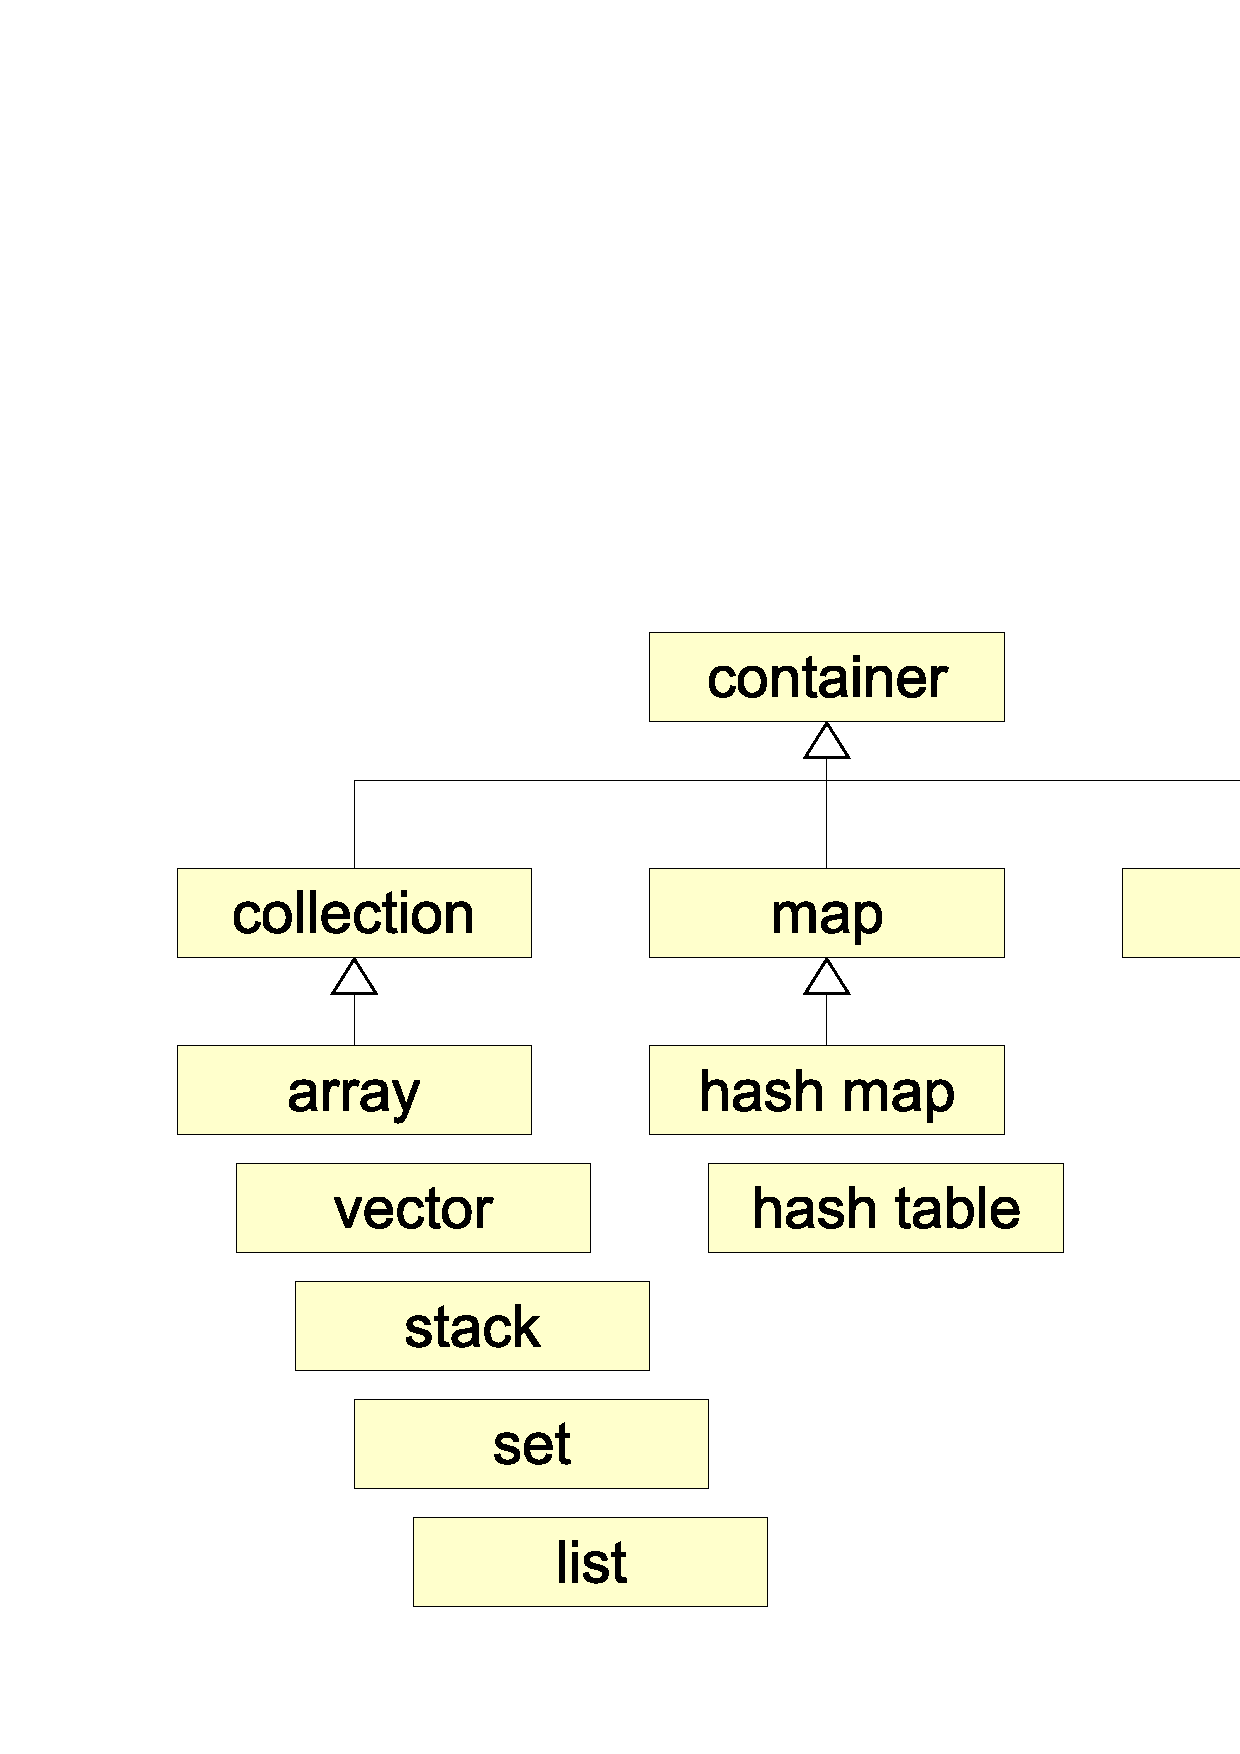
\includegraphics[scale=0.3,angle=-90]{graphic/container.pdf}
        \caption{Java Container Framework Systematics}
        \label{container_figure}
    \end{center}
\end{figure}

One way to store references to more than one dynamic element in memory, or
primitive data, is a \emph{Container}. Modern programming languages offer many
different kinds of containers. Figure \ref{container_figure} shows a
systematics of the Java container framework \cite{java}, as example, which gets
briefly introduced in the following paragraphs. Its main categories of
systematisation are \emph{Collection}, \emph{Map} and \emph{Tree}.

A similar library of container classes, algorithms and iterators exists for the
C++ programming language. It is called \emph{Standard Template Library} (STL)
\cite{stl} and it talks of \emph{Sequence} and \emph{Associative Container},
where Java says \emph{Collection} and \emph{Map}.

\input{collection}
\input{map}
\input{tree}

%
% $RCSfile: falsifying_polymorphism.tex,v $
%
% Copyright (C) 2002-2008. Christian Heller.
%
% Permission is granted to copy, distribute and/or modify this document
% under the terms of the GNU Free Documentation License, Version 1.1 or
% any later version published by the Free Software Foundation; with no
% Invariant Sections, with no Front-Cover Texts and with no Back-Cover
% Texts. A copy of the license is included in the section entitled
% "GNU Free Documentation License".
%
% http://www.cybop.net
% - Cybernetics Oriented Programming -
%
% http://www.resmedicinae.org
% - Information in Medicine -
%
% Version: $Revision: 1.1 $ $Date: 2008-08-19 20:41:06 $ $Author: christian $
% Authors: Christian Heller <christian.heller@tuxtax.de>
%

\subsubsection{Falsifying Polymorphism}
\label{falsifying_polymorphism_heading}
\index{Falsifying Polymorphism}
\index{Container Inheritance}
\index{Hashtable}
\index{Copy Constructor}

Problems can occur when inheriting containers. This is now demonstrated on a Java
example adopted from \cite{javaiaq}.

\begin{figure}[ht]
    \begin{center}
        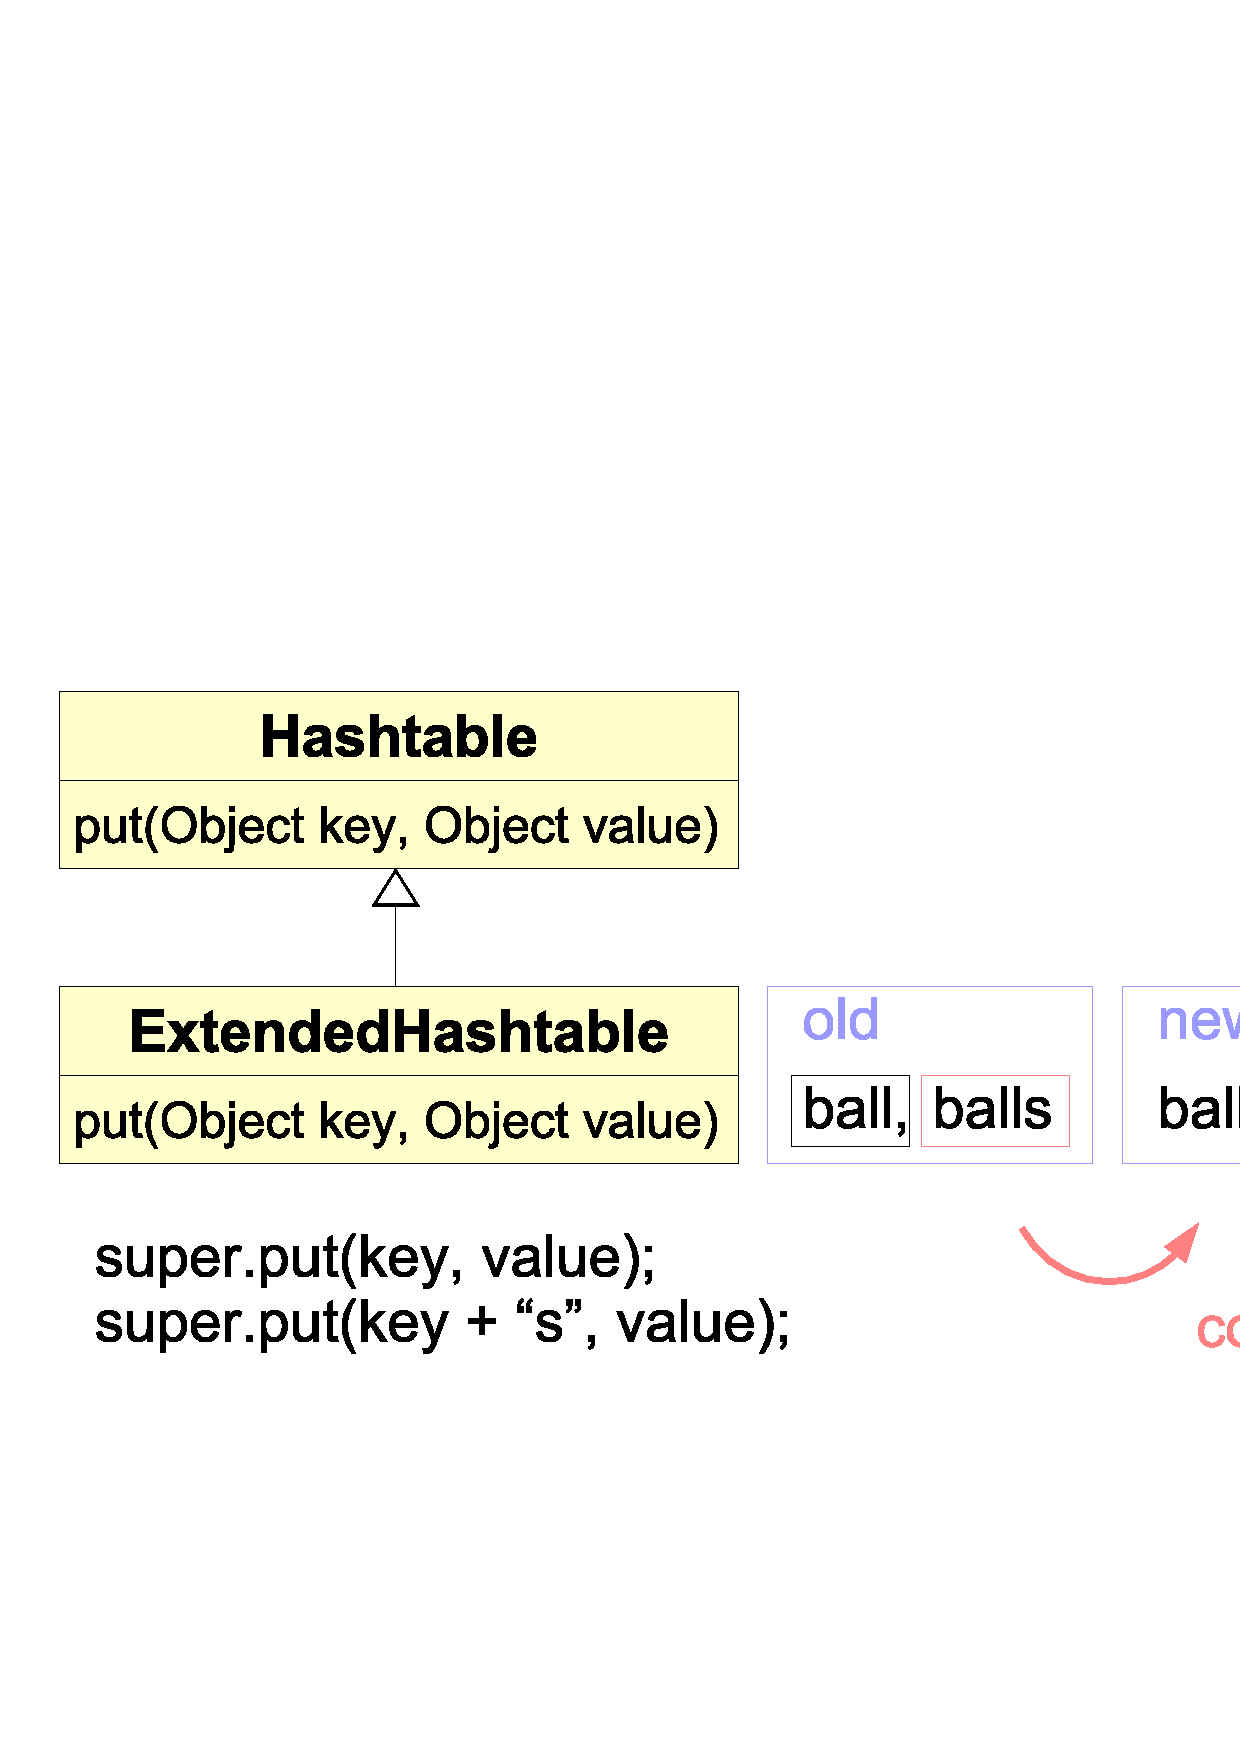
\includegraphics[scale=0.3,angle=-90]{graphic/falsifying.pdf}
        \caption{Falsified Contents with Container Inheritance}
        \label{falsifying_figure}
    \end{center}
\end{figure}

A class \emph{ExtendedHashtable} extends the standard container \emph{Hashtable}
(figure \ref{falsifying_figure}). The \emph{ExtendedHashtable} overrides the
\emph{put} method and lets it do two calls to the \emph{put} method of the
superior class \emph{Hashtable}, the second of these calls adding the letter
\emph{s} to the key.

A first object of type \emph{ExtendedHashtable} gets filled by calling the
\emph{put} method which adds two identical element values with the two different
keys \emph{ball} and \emph{balls} to the container. When the container is full,
a new one with extended size gets created and all values of the old have to be
copied into the new container, which is again of type \emph{ExtendedHashtable}.

If the \emph{put} method is now used to accomplish this, a falsified container
with more elements than the original one will be retrieved. The copying of the
first element \emph{ball} results in two elements \emph{ball} and \emph{balls},
placed in the new container. The copying of the second element \emph{balls} adds
two further elements \emph{balls} and \emph{ballss}, whereby the \emph{balls}
key stemming from the copying of the first element gets overwritten.

This example demonstrates only the principle of how the automatic size
extension of inherited container objects with element copying using
container-owned methods can incorrectly modify the container contents. The Java
language's \emph{Hashtable} class uses a slightly different mechanism, handing
over the hashtable object as parameter of a copy constructor which internally
calls a \emph{putAll} method which finally calls the \emph{put} method. Other
OOP languages may use different mechanisms. Of course, there are workarounds to
avoid the described troubles. But as a matter of fact, container inheritance
may -- due to polymorphism -- cause unpredictable behaviour leading to
\emph{falsified} container contents.

The language and interpreter introduced in chapters
\ref{cybernetics_oriented_language_heading} and
\ref{cybernetics_oriented_interpreter_heading} base on just one container
structure for knowledge representation, that covers many of the traditional
forms of containers.

%
% $RCSfile: conclusion.tex,v $
%
% Copyright (C) 2002-2008. Christian Heller.
%
% Permission is granted to copy, distribute and/or modify this document
% under the terms of the GNU Free Documentation License, Version 1.1 or
% any later version published by the Free Software Foundation; with no
% Invariant Sections, with no Front-Cover Texts and with no Back-Cover
% Texts. A copy of the license is included in the section entitled
% "GNU Free Documentation License".
%
% http://www.cybop.net
% - Cybernetics Oriented Programming -
%
% http://www.resmedicinae.org
% - Information in Medicine -
%
% Version: $Revision: 1.1 $ $Date: 2008-08-19 20:41:06 $ $Author: christian $
% Authors: Christian Heller <christian.heller@tuxtax.de>
%

\subsubsection{Conclusion}
\label{conclusion_heading}
\index{OOP Innovations}
\index{Object Oriented Programming}
\index{OOP}
\index{Structured and Procedural Programming}
\index{SPP}

As could be seen in the previous sections, OOP contributed many new concepts
to software design, thus trying to improve SPP. Most importantly, SPP data
structures (struct, record) got extended towards the \emph{Class} which does
not only hold data (attributes), but also operations (methods). This brought
with the concept of \emph{Encapsulation}, which permits only special methods of
an \emph{Object} (class instance) to access the data (properties) of that same
object. The next innovation was \emph{Inheritance}, which allows a class to
reuse the attributes and methods of its super class(es). Finally, inheritance
was used to introduce the concept of \emph{Polymorphism}, which lets objects
react differently, depending on the class they were instantiated with.

All of these concepts were true innovations as compared with traditional SPP
techniques. However, they have their own drawbacks: growth of the number of
dependencies within a system (links between classes), caused by the bundling of
attributes and methods; fragile base class problem; falsified container
contents with container inheritance. This work will not just revise these
concepts, but turn them upside down. Data (attributes) and operations/
algorithms (methods) are not bundled any longer; the resolution of inheritance
relationships at runtime gets eliminated and with it polymorphism; container
inheritance is not necessary any longer, since only one global container
structure (knowledge container) is used in a system. More on that in part
\ref{contribution_heading} of this work.



%
% $RCSfile: pattern.tex,v $
%
% Copyright (c) 2004. Christian Heller. All rights reserved.
%
% No copying, altering, distribution or any other actions concerning this
% document, except after explicit permission by the author!
% At some later point in time, this document is planned to be put under
% the GNU FDL license. For now, _everything_ is _restricted_ by the author.
%
% http://www.cybop.net
% - Cybernetics Oriented Programming -
%
% http://www.resmedicinae.org
% - Information in Medicine -
%
% @author Christian Heller <christian.heller@tuxtax.de>
%

\section{Pattern}
\label{pattern_heading}

%
% $RCSfile: definition.tex,v $
%
% Copyright (c) 2002-2007. Christian Heller. All rights reserved.
%
% Permission is granted to copy, distribute and/or modify this document
% under the terms of the GNU Free Documentation License, Version 1.1 or
% any later version published by the Free Software Foundation; with no
% Invariant Sections, with no Front-Cover Texts and with no Back-Cover
% Texts. A copy of the license is included in the section entitled
% "GNU Free Documentation License".
%
% http://www.cybop.net
% - Cybernetics Oriented Programming -
%
% Version: $Revision: 1.2 $ $Date: 2007-08-01 13:59:00 $ $Author: christian $
% Authors: Christian Heller <christian.heller@tuxtax.de>
%

\chapter{Definition}
\label{definition_heading}
\index{Definition}
\index{Whole-Part Hierarchy}
\index{Meta Data Hierarchy}
\index{Extensible Markup Language}
\index{XML}

This chapter defines the \emph{Syntax}, \emph{Vocabulary} and \emph{Semantics}
of the CYBOL language.

As already mentioned in chapter \ref{introduction_heading}, CYBOL is based upon
\emph{two} kinds of hierarchies. One of them is representing \emph{Whole-Part}
relations (such as a graphical window consisting of a menu bar) and the other
the \emph{Meta Data} which a whole keeps about its parts (such as the size or
colour of the menu bar). More details and the philosophical background are
described in \cite{cybopbook}. The syntax and semantics of CYBOL as new
language must be rich enough to express abstract knowledge models using this
kind of double hierarchy.

%
% $RCSfile: syntax.tex,v $
%
% Copyright (C) 2002-2008. Christian Heller.
%
% Permission is granted to copy, distribute and/or modify this document
% under the terms of the GNU Free Documentation License, Version 1.1 or
% any later version published by the Free Software Foundation; with no
% Invariant Sections, with no Front-Cover Texts and with no Back-Cover
% Texts. A copy of the license is included in the section entitled
% "GNU Free Documentation License".
%
% http://www.cybop.net
% - Cybernetics Oriented Programming -
%
% http://www.resmedicinae.org
% - Information in Medicine -
%
% Version: $Revision: 1.1 $ $Date: 2008-08-19 20:41:09 $ $Author: christian $
% Authors: Christian Heller <christian.heller@tuxtax.de>
%

\subsection{Syntax}
\label{syntax_heading}
\index{CYBOL Syntax}
\index{Syntax of a Language}
\index{Grammar of a Language}
\index{Extensible Markup Language}
\index{XML}
\index{XML Tag}
\index{XML Attribute}
\index{Discrimination}
\index{Composition}

Every language has a special \emph{Syntax}, that is a \emph{Grammar} with rules
for combining terms and symbols \cite{foldoc}. CYBOL could define its own
syntax or use an already existing one, of another language. Because of its
popularity, clear text representation, flexibility, extensibility and ease of
use, \emph{XML} was chosen to deliver the syntax for CYBOL.

To mention just two of the syntactical elements of XML, \emph{Tag} and
\emph{Attribute} are considered shortly here. Tags are special, arbitrary
keywords that have to be defined by the system working with an XML document.
Attributes keep additional information about the contents enclosed by two tags.
Two examples:

\begin{scriptsize}
    \begin{verbatim}
    <tag attribute="value">
        contents
    </tag>
    \end{verbatim}
\end{scriptsize}

\begin{scriptsize}
    \begin{verbatim}
    <tag attribute1="value" attribute2="contents"/>
    \end{verbatim}
\end{scriptsize}

An XML document carries a name and can such represent a \emph{Discrete Item},
as suggested by the principles of human thinking (section
\ref{human_thinking_heading}). Being a \emph{Compound}, it consists of parts --
and, it can link to other documents treated as its parts. That way, a whole
hierarchy can be formed. Tag attributes can keep additional information about
the linked parts. Most importantly, XML documents have a hierarchical structure
based on tags, which may be used to store meta information about a part.

Considering these properties of XML, it seems predestinated for formally
representing abstract models using the CYBOP concepts. CYBOL, finally, is XML
\emph{plus} a defined set of tags, attributes and values, used to structure and
link documents meaningfully.

%
% $RCSfile: vocabulary.tex,v $
%
% Copyright (c) 2001-2004. Christian Heller. All rights reserved.
%
% No copying, altering, distribution or any other actions concerning this
% document, except after explicit permission by the author!
% At some later point in time, this document is planned to be put under
% the GNU FDL license. For now, _everything_ is _restricted_ by the author.
%
% http://www.cybop.net
% - Cybernetics Oriented Programming -
%
% http://www.resmedicinae.org
% - Information in Medicine -
%
% @author Christian Heller <christian.heller@tuxtax.de>
%

\subsection{Vocabulary}
\label{vocabulary_heading}

XML allows to define and exchange the whole vocabulary of a language. It offers
two ways in which a list of legal elements can be defined: The traditional
\emph{Document Type Definition} (DTD) and the more modern \emph{XML Schema
Definition} (XSD). Besides the vocabulary, DTD and XSD define the structure of
an XML document and allow to typify, constrain and validate items. The CYBOL DTD
and XSD can be found at \cite{cybop}.

%
% $RCSfile: semantics.tex,v $
%
% Copyright (c) 2002-2007. Christian Heller. All rights reserved.
%
% Permission is granted to copy, distribute and/or modify this document
% under the terms of the GNU Free Documentation License, Version 1.1 or
% any later version published by the Free Software Foundation; with no
% Invariant Sections, with no Front-Cover Texts and with no Back-Cover
% Texts. A copy of the license is included in the section entitled
% "GNU Free Documentation License".
%
% http://www.cybop.net
% - Cybernetics Oriented Programming -
%
% Version: $Revision: 1.1 $ $Date: 2007-08-01 13:59:00 $ $Author: christian $
% Authors: Christian Heller <christian.heller@tuxtax.de>
%

\section{Semantics}
\label{semantics_heading}
\index{Semantics}
\index{State Knowledge Modelling}
\index{Logic Knowledge Modelling}
\index{Extensible Markup Language}
\index{XML}
\index{XML Tag}
\index{XML Attribute}

The meaning expressed by terms and sentences is their \emph{Semantics}
\cite{duden}.

CYBOL files can be used to model \emph{State Knowledge} (like a graphical
window or a person's address) and \emph{Logic Knowledge} (like an operation or
algorithm or workflow) \cite{cybopbook}. In both cases, the \emph{same} syntax
(document structure) with \emph{identical} vocabulary (XML tags and -attributes)
is applied. It is the attribute \emph{Values} that make a difference in meaning.

The double hierarchy mentioned before is realised in CYBOL knowledge templates
by using XML \emph{Attributes} for representing the whole-part hierarchy, and
XML \emph{Tags} for representing the additional meta data that a whole model
keeps about its part models.

\input{attributes}
\input{tags}
\input{tag_attribute_swapping}


%
% $RCSfile: classification.tex,v $
%
% Copyright (C) 2002-2008. Christian Heller.
%
% Permission is granted to copy, distribute and/or modify this document
% under the terms of the GNU Free Documentation License, Version 1.1 or
% any later version published by the Free Software Foundation; with no
% Invariant Sections, with no Front-Cover Texts and with no Back-Cover
% Texts. A copy of the license is included in the section entitled
% "GNU Free Documentation License".
%
% http://www.cybop.net
% - Cybernetics Oriented Programming -
%
% http://www.resmedicinae.org
% - Information in Medicine -
%
% Version: $Revision: 1.1 $ $Date: 2008-08-19 20:41:05 $ $Author: christian $
% Authors: Christian Heller <christian.heller@tuxtax.de>
%

\subsubsection{Classification}
\label{classification_heading}
\index{Classification}
\index{Class}
\index{Attribute}
\index{Method}
\index{Structured Data Type}
\index{Struct}
\index{Record}
\index{Structured and Procedural Programming}
\index{SPP}
\index{Java}
\index{Global Variable}
\index{Instance}
\index{Object}
\index{Instantiation}
\index{Abstract Class}
\index{Interface}
\index{Inner Class}
\index{Bundling of Attributes and Methods}

The main idea of object oriented programming is to structure program code into
\emph{Classes} owning \emph{Attributes} and \emph{Methods} (figure
\ref{classification_figure}). They are comparable to the structured data types
(\emph{struct}, \emph{record}) of \emph{Structured and Procedural Programming}
(SPP) (section \ref{structured_and_procedural_programming_heading}) that can
own fields representing properties, but not behaviour. A class definition in
\emph{Java} source code looks like this:

\begin{scriptsize}
    \begin{verbatim}
    public class Example {
        private Type attribute;
        public void method(Type parameter) {
        }
    }
    \end{verbatim}
\end{scriptsize}

\begin{figure}[ht]
    \begin{center}
        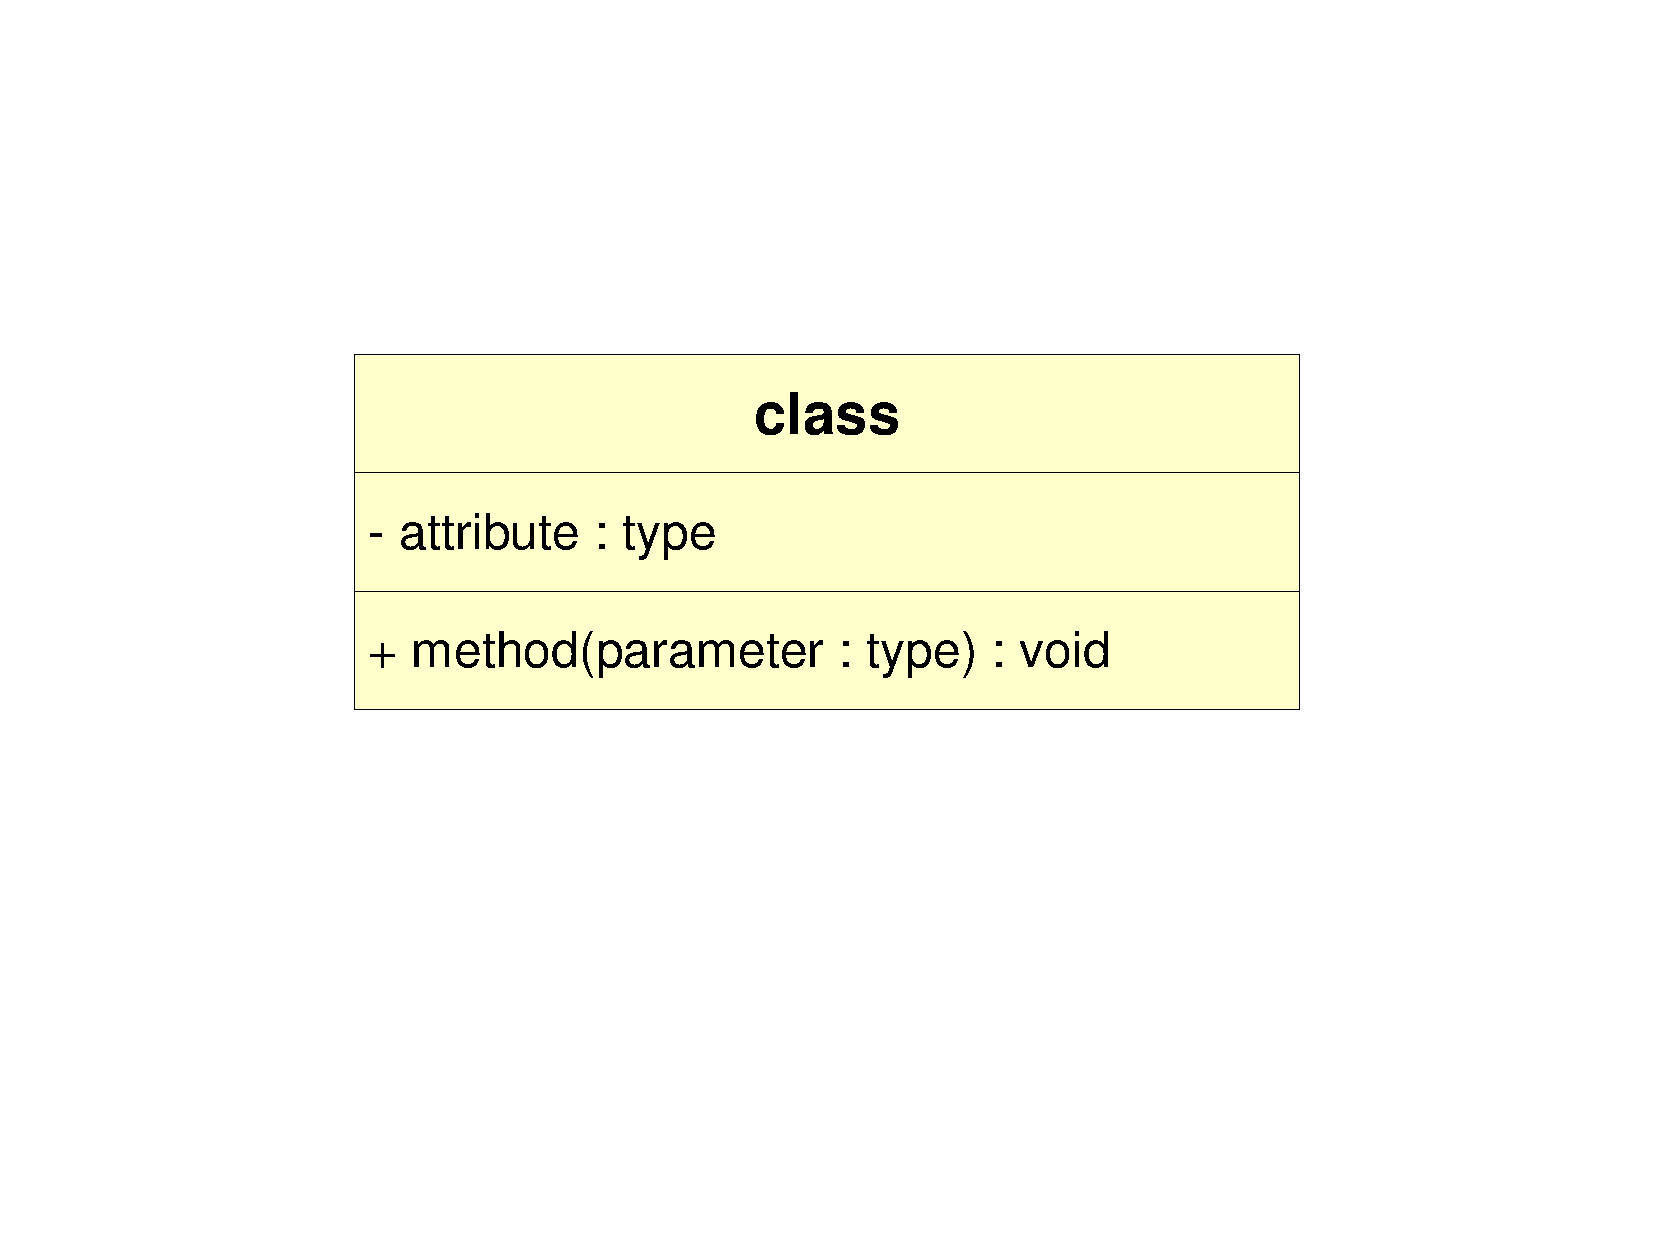
\includegraphics[scale=0.3,angle=-90]{graphic/classification.pdf}
        \caption{Classification as UML Diagram}
        \label{classification_figure}
    \end{center}
\end{figure}

While procedures and many variables in SPP are global, that is only exist once,
classes are treated as types of which many \emph{Instances} (also called
\emph{Objects}) can be created, including attributes and methods. In OOP, such
memory allocation is called \emph{Instantiation}.

Two related data types are \emph{Abstract Class} and \emph{Interface}. An
abstract class can hold attributes and (partly abstract) methods. Just like
interfaces, abstract classes cannot be instantiated. An interface is yet more
restricted in that it can only have constants but not attributes and only
declarations but not actual implementations of methods. Interfaces are commonly
used to \cite{steppan}:

\begin{itemize}
    \item[-] Realise multiple inheritance (section \ref{inheritance_heading})
    \item[-] Encapsulate components (section \ref{interface_and_implementation_heading})
    \item[-] Pool common methods (section \ref{separation_of_concerns_heading})
\end{itemize}

Specialities like \emph{Inner Classes} \cite{java} with limited scope of
validity are of minor importance to the argumentation of this document and not
further explained here.

The \emph{Bundling} of attributes and methods (state and logic) causes more
system interdependencies and complications than were predictable. It is a big
disadvantage that affects all modern object-oriented systems. \cite{heller2004}
Certainly, the bundling stems from best intentions to receive cleaner code by
keeping not only attributes but also methods in a common module, such avoiding
\emph{wild} and \emph{global} procedures. But now, modules not only have to
refer to other modules for accessing their state data; the same is needed for
accessing their logic in form of method calls.

With OOP, the number of cross-relations between modules, and inter-dependencies
between system layers may rise dramatically. In reality, state- and logic
properties are two \emph{different} things that have to be kept in different
places! Both can have a similar, hierarchical structure but each is a concept on
its own, as chapter \ref{state_and_logic_heading} will show.

%
% $RCSfile: examples.tex,v $
%
% Copyright (c) 2002-2007. Christian Heller. All rights reserved.
%
% Permission is granted to copy, distribute and/or modify this document
% under the terms of the GNU Free Documentation License, Version 1.1 or
% any later version published by the Free Software Foundation; with no
% Invariant Sections, with no Front-Cover Texts and with no Back-Cover
% Texts. A copy of the license is included in the section entitled
% "GNU Free Documentation License".
%
% http://www.cybop.net
% - Cybernetics Oriented Programming -
%
% Version: $Revision: 1.1 $ $Date: 2007-08-01 13:59:00 $ $Author: christian $
% Authors: Christian Heller <christian.heller@tuxtax.de>
%

\chapter{Examples}
\label{examples_heading}
\index{Examples}

The following examples demonstrate how CYBOL's constructs may be used in
practice. Also, attention is payed to how control structures of classical
programming languages may be implemented in CYBOL. Furthermore, this section
discusses how inheritance, containers and software patterns were considered in
the design of CYBOL.

%
% $RCSfile: state_examples.tex,v $
%
% Copyright (C) 2002-2008. Christian Heller.
%
% Permission is granted to copy, distribute and/or modify this document
% under the terms of the GNU Free Documentation License, Version 1.1 or
% any later version published by the Free Software Foundation; with no
% Invariant Sections, with no Front-Cover Texts and with no Back-Cover
% Texts. A copy of the license is included in the section entitled
% "GNU Free Documentation License".
%
% http://www.cybop.net
% - Cybernetics Oriented Programming -
%
% http://www.resmedicinae.org
% - Information in Medicine -
%
% Version: $Revision: 1.1 $ $Date: 2008-08-19 20:41:09 $ $Author: christian $
% Authors: Christian Heller <christian.heller@tuxtax.de>
%

\subsection{State Examples}
\label{state_examples_heading}
\index{CYBOL State Example Constructs}

The creation of composed state models is quite straightforward and clear, as
the following CYBOL knowledge templates show.

\input{model_part_relation}
\input{meta_properties}
\input{external_resources}
\input{serialised_model}
\input{meta_constraints}

%
% $RCSfile: logic_examples.tex,v $
%
% Copyright (C) 2002-2008. Christian Heller.
%
% Permission is granted to copy, distribute and/or modify this document
% under the terms of the GNU Free Documentation License, Version 1.1 or
% any later version published by the Free Software Foundation; with no
% Invariant Sections, with no Front-Cover Texts and with no Back-Cover
% Texts. A copy of the license is included in the section entitled
% "GNU Free Documentation License".
%
% http://www.cybop.net
% - Cybernetics Oriented Programming -
%
% http://www.resmedicinae.org
% - Information in Medicine -
%
% Version: $Revision: 1.1 $ $Date: 2008-08-19 20:41:07 $ $Author: christian $
% Authors: Christian Heller <christian.heller@tuxtax.de>
%

\subsection{Logic Examples}
\label{logic_examples_heading}
\index{CYBOL Logic Example Constructs}

The CYBOL implementation of logic models (chapter \ref{state_and_logic_heading})
needs more detailed explanation, in particular the use of special control
structures as known from \emph{Structured and Procedural Programming} (SPP)
(section \ref{structured_and_procedural_programming_heading}).

\input{operation_call}
\input{algorithm_division}
\input{simple_assignment}
\input{loop_as_operation}
\input{conditional_execution}

%
% $RCSfile: special_examples.tex,v $
%
% Copyright (C) 2002-2008. Christian Heller.
%
% Permission is granted to copy, distribute and/or modify this document
% under the terms of the GNU Free Documentation License, Version 1.1 or
% any later version published by the Free Software Foundation; with no
% Invariant Sections, with no Front-Cover Texts and with no Back-Cover
% Texts. A copy of the license is included in the section entitled
% "GNU Free Documentation License".
%
% http://www.cybop.net
% - Cybernetics Oriented Programming -
%
% http://www.resmedicinae.org
% - Information in Medicine -
%
% Version: $Revision: 1.1 $ $Date: 2008-08-19 20:41:09 $ $Author: christian $
% Authors: Christian Heller <christian.heller@tuxtax.de>
%

\subsection{Special Examples}
\label{special_examples_heading}
\index{CYBOL Special Example Constructs}

\emph{XML} is used for representing data of very different domains, and a whole
plethora of XML dialects exists. Two of them are mentioned following. The main
purpose of the next examples, however, is to show how CYBOL can replace these.

\input{synchronous_execution}
\input{presentation_and_content}
\input{hello_world}
\input{any_system}

%
% $RCSfile: inheritance_as_property.tex,v $
%
% Copyright (c) 2002-2007. Christian Heller. All rights reserved.
%
% Permission is granted to copy, distribute and/or modify this document
% under the terms of the GNU Free Documentation License, Version 1.1 or
% any later version published by the Free Software Foundation; with no
% Invariant Sections, with no Front-Cover Texts and with no Back-Cover
% Texts. A copy of the license is included in the section entitled
% "GNU Free Documentation License".
%
% http://www.cybop.net
% - Cybernetics Oriented Programming -
%
% Version: $Revision: 1.1 $ $Date: 2007-08-01 13:59:00 $ $Author: christian $
% Authors: Christian Heller <christian.heller@tuxtax.de>
%

\section{Inheritance as Property}
\label{inheritance_as_property_heading}
\index{Inheritance as CYBOL Property}

One fundamental concept of \emph{Object Oriented Programming} (OOP) is
\emph{Inheritance}. In principle, there is no problem with implementing
inheritance in CYBOL. If done, however, it would differ from traditional class
architectures as known from OOP. Classical OOP systems resolve inheritance
relationships at runtime; CYBOP systems, on the other hand, would resolve them
just once when creating a knowledge model (instance) from a knowledge template.
After instantiation, all inheritance relationships are lost since instances are
stored as purely hierarchical \emph{whole}-\emph{part} models in memory,
without any links to \emph{super} models.

The following knowledge template shows how inheritance could be realised in
CYBOL. Contrary to OOP classes which hold a link to their corresponding
\emph{super} class as \emph{intrinsic} property, a CYBOL knowledge template
does not know itself from which \emph{super} template to inherit from. That
information is stored as \emph{extrinsic} property outside the template
instead, in other words in the \emph{whole} template to which the inheriting
template belongs.

\begin{scriptsize}
    \begin{verbatim}
<model>
    <part name="ok_button" channel="file" abstraction="cybol" model="gui/ok_button.cybol">
        <property name="super" channel="file" abstraction="cybol" model="button.cybol"/>
        <property name="size" channel="inline" abstraction="integer" model="90,30,1"/>
        <property name="colour" channel="inline" abstraction="rgb" model="127,127,127"/>
    </part>
</model>
    \end{verbatim}
\end{scriptsize}

One of the properties in the example template above carries the name
\emph{super}. Its model references another template which is treated as super
template of the corresponding \emph{part} the property belongs to. With slight
modifications on the property name \emph{super}, which has to be unique among
all properties of a part, it would even be possible to implement
\emph{Multiple Inheritance}. Dependency complications are not to be expected
because all inheritance relationships are forgotten in runtime models.

Although the described inheritance mechanism was tested successfully in an
older prototype application, it has not been implemented in CYBOL. None of the
created example applications showed a need for it, nor did any of them promise
more effective programming. The reuse of CYBOL templates is realised through
composition only, that is fine-granular templates make up more coarse-grained
ones. This counts for both, state- as well as logic models, since they are not
bundled like in OOP. And polymorphism as effect does not have to be considered.

%
% $RCSfile$
%
% Copyright (c) 2005-2006. Christian Heller. All rights reserved.
%
% Permission is granted to copy, distribute and/or modify this document
% under the terms of the GNU Free Documentation License, Version 1.1 or
% any later version published by the Free Software Foundation; with no
% Invariant Sections, with no Front-Cover Texts and with no Back-Cover
% Texts. A copy of the license is included in the section entitled
% "GNU Free Documentation License".
%
% http://www.cybop.net
% - Cybernetics Oriented Programming -
%
% http://www.resmedicinae.org
% - Information in Medicine -
%
% Version: $Revision$ $Date$ $Author$
% Authors: Christian Heller <christian.heller@tuxtax.de>
%

\subsubsection{Container Mapping}
\label{container_mapping_heading}

State-of-the-art programming languages offer a number of different container
types, partly based on each other through inheritance. Sections
\ref{motivation_heading} and \ref{container_unification_heading} of this work
mentioned \emph{Container Inheritance} as one reason for falsified program
results.

\begin{table}[ht]
    \begin{center}
        \begin{tabular}{| p{15mm} | p{35mm} |}
            \hline
            \textbf{Container} & \textbf{Knowledge Template}\\
            \hline
            Tree & Hierarchical \emph{whole}-\emph{part} structure\\
            \hline
            Table & Like a Tree, as hierarchy consisting of rows which consist of columns\\
            \hline
            Map & Parts have a \emph{name} (key) and a \emph{model} (value)\\
            \hline
            List & Parts may have a \emph{position} property\\
            \hline
            Vector & A \emph{model} attribute may hold comma-separated values;
                a template holds a number of parts (dynamically changeable)\\
            \hline
            Array & Like a Vector; characters are interpreted as \emph{string}\\
            \hline
        \end{tabular}
        \caption{Containers in CYBOL}
        \label{mapping_table}
    \end{center}
\end{table}

Section \ref{knowledge_schema_heading} introduced a \emph{Knowledge Schema}
which represents each item as \emph{Hierarchy} by default, the result being
that different types of containers are not needed any longer. But how are the
different kinds of container behaviour implemented in CYBOL? Table
\ref{mapping_table} gives an answer.

%
% $RCSfile: hidden_patterns.tex,v $
%
% Copyright (C) 2002-2008. Christian Heller.
%
% Permission is granted to copy, distribute and/or modify this document
% under the terms of the GNU Free Documentation License, Version 1.1 or
% any later version published by the Free Software Foundation; with no
% Invariant Sections, with no Front-Cover Texts and with no Back-Cover
% Texts. A copy of the license is included in the section entitled
% "GNU Free Documentation License".
%
% http://www.cybop.net
% - Cybernetics Oriented Programming -
%
% http://www.resmedicinae.org
% - Information in Medicine -
%
% Version: $Revision: 1.1 $ $Date: 2008-08-19 20:41:07 $ $Author: christian $
% Authors: Christian Heller <christian.heller@tuxtax.de>
%

\subsection{Hidden Patterns}
\label{hidden_patterns_heading}
\index{Patterns in CYBOL}
\index{Hidden Patterns in CYBOL}

There are a number of software patterns (section \ref{pattern_heading}) that
may not be obvious (hidden) at first sight, but have been considered in the
design of the CYBOL language.

Most obviously, CYBOL knowledge templates follow the \emph{Composite} pattern,
in a simplified form. All templates represent a compound consisting of part
templates, which leads to a tree-like structure. But this also means that related
patterns (see section \ref{pattern_systematics_heading}) like \emph{Whole-Part}
and \emph{Wrapper} are representable by CYBOL knowledge templates. A template
as whole wraps its parts.

Knowledge templates with similar granularity can be collected in one directory,
in other words one common ontological level. Templates with smaller granularity,
that is those that the more coarse-grained templates consist of, can be placed
in another common layer and so forth. What comes out of it is a system of levels
-- one variant of the \emph{Layers} pattern.



%
% $RCSfile: component_oriented_programming.tex,v $
%
% Copyright (C) 2002-2008. Christian Heller.
%
% Permission is granted to copy, distribute and/or modify this document
% under the terms of the GNU Free Documentation License, Version 1.1 or
% any later version published by the Free Software Foundation; with no
% Invariant Sections, with no Front-Cover Texts and with no Back-Cover
% Texts. A copy of the license is included in the section entitled
% "GNU Free Documentation License".
%
% http://www.cybop.net
% - Cybernetics Oriented Programming -
%
% http://www.resmedicinae.org
% - Information in Medicine -
%
% Version: $Revision: 1.1 $ $Date: 2008-08-19 20:41:06 $ $Author: christian $
% Authors: Christian Heller <christian.heller@tuxtax.de>
%

\section{Component Oriented Programming}
\label{component_oriented_programming_heading}
\index{Component Oriented Programming}
\index{COP}
\index{Component Based Design}
\index{CBD}
\index{Software Component}
\index{Component}
\index{Black Box Reuse}
\index{Graphical User Interface}
\index{GUI}
\index{Delphi}
\index{Visual Component Library}
\index{VCL}
\index{Visual Basic}
\index{VB}
\index{Java}
\index{Abstract Window Toolkit}
\index{AWT}
\index{Bean}
\index{Agent}
\index{Open Source Software}
\index{OSS}
\index{Legacy System}
\index{PL/1}
\index{Interface Definition Language}
\index{IDL}
\index{Common Object Request Broker Architecture}
\index{CORBA}
\index{Aspect Oriented Programming}
\index{AOP}
\index{Aspect}
\index{Concern}
\index{Agent Oriented Programming}
\index{AGOP}
\index{Agent}

In the not-so-distant past, there has been a lot of buzz in the industry
touting \emph{Component Based Design} (CBD). Much of it was more marketing than
the actual application of new design principles and it is also no surprise that
the definition of a \emph{Software Component} differs between authors, companies
and projects. A rather formal one is that of the \emph{Avalon} framework
\cite{avalon} of the \emph{Apache Jakarta} project \cite{jakarta}, which says:

\begin{quote}
    \emph{Component Oriented Programming} takes object-oriented programming one
    step further. Regular object-oriented programming organizes data objects
    into entities that take care of themselves. There are many advantages to
    this approach. \ldots\ But it also has a big limitation: that of object
    \emph{Co-Dependency}. To remove that limitation, a more rigid idea had to
    be formalized: the \emph{Component}. The key difference between a regular
    object and a component is that a component is completely replaceable
    (\emph{Black Box Reuse}).
\end{quote}

Many kinds of software components exist: There are \emph{Graphical User Interface}
(GUI) components known from Delphi's \emph{Visual Component Library} (VCL)
\cite{delphi}, from \emph{Visual Basic} (VB) \cite{visualbasic} or Java's
\emph{Abstract Window Toolkit} (AWT) \cite{java}, which calls its components
\emph{Beans}; there are \emph{Business} components containing domain knowledge
and \emph{Technical} components interacting with infrastructure systems like
\emph{CORBA-}/ \emph{EJB-}/ \emph{DCOM} middleware, with a \emph{Database} (DB)
or \emph{Operating System} (OS) (sections \ref{database_server_heading},
\ref{remote_server_heading}); there are general \emph{Application} components
as investigated by \emph{Avalon} \cite{avalon}. Whole systems, that is
self-acting components, are often called \emph{Agents} (section
\ref{agent_oriented_programming_heading}).

The following sections deal with application components whose principles are
investigated on the example of the \emph{Avalon} framework, because that is an
\emph{Open Source Software} (OSS) project providing all sources for free. After
\emph{Avalon} \cite{avalon}, \emph{Component Oriented Programming} (COP) were
not necessarily the same as \emph{Component Based Design} (CBD). The latter
referred to how a system is \emph{designed}; the former to how it is
\emph{implemented}. In practice, one could not implement COP without first
designing with components in mind.

By following CBD rules, software projects try to integrate most diverse systems
into one environment. Although the systems should ideally use COP for the
implementation of their components, this is not a must. Legacy systems (section
\ref{legacy_host_heading}) can be encapsulated as well \cite{brown2000}, acting
as one component to the outside environment. A \emph{Service} offered by a legacy
system written in \emph{PL/1} \cite{pli}, for example, may be designed and
treated as component. It may be accessed via \emph{Interface Definition Language}
(IDL) interfaces and use a \emph{Common Object Request Broker Architecture}
(CORBA) for communication. The interna of such a system, however, do neither
have to follow component- nor object-oriented programming principles.

The following sections describe popular COP techniques. Although being
researched in an own scientific field, \emph{Aspect Oriented Programming} (AOP)
principles are added as sub-section, because \emph{Aspects} are comparable to
the \emph{Concerns} of COP. For similar reasons, \emph{Agent Oriented Programming}
(AGOP) techniques are described following, because \emph{Agents} can be seen as
self-acting \emph{Components}. All of them, that is COP's concerns, AOP's
aspects and AGOP's agents owning a knowledge base will be recalled once again
in part \ref{contribution_heading} of this work.

%
% $RCSfile: inversion_of_control.tex,v $
%
% Copyright (C) 2002-2008. Christian Heller.
%
% Permission is granted to copy, distribute and/or modify this document
% under the terms of the GNU Free Documentation License, Version 1.1 or
% any later version published by the Free Software Foundation; with no
% Invariant Sections, with no Front-Cover Texts and with no Back-Cover
% Texts. A copy of the license is included in the section entitled
% "GNU Free Documentation License".
%
% http://www.cybop.net
% - Cybernetics Oriented Programming -
%
% http://www.resmedicinae.org
% - Information in Medicine -
%
% Version: $Revision: 1.1 $ $Date: 2008-08-19 20:41:07 $ $Author: christian $
% Authors: Christian Heller <christian.heller@tuxtax.de>
%

\subsection{Inversion of Control}
\label{inversion_of_control_heading}
\index{Inversion of Control Pattern}
\index{IoC}
\index{Component}
\index{Application Programming Interface}
\index{API}
\index{Framework}
\index{Observer Pattern}
\index{Chain of Responsibility Pattern}
\index{Bidirectional Dependency}
\index{Strong Coupling}
\index{Dependency Injection}
\index{Unidirectional Dependency}
\index{Security by Design}
\index{Container}
\index{Component Isolation}
\index{Component Lifecycle}

The \emph{Avalon} documentation \cite{avalon} defines a \emph{Component} as
\emph{a passive entity that performs a specific role}. According to this
definition, a passive entity has to employ a \emph{passive}
\emph{Application Programming Interface} (API) which, after \cite{avalon}, were
one that is acted upon, versus one that acts itself.

As could be seen in section \ref{framework_heading}, it is often desirable to
let a framework play the role of the main program coordinating and sequencing
events and application activity. \emph{Observers} (section \ref{observer_heading})
are applied to realise a callback mechanism; a \emph{Chain of Responsibility}
(section \ref{chain_of_responsibility_heading}) is often set up among objects
so that they can react to certain messages in a delegation hierarchy. Both
patterns rely on bidirectional dependencies whose negative effects such as
\emph{Strong Coupling} were mentioned before (section
\ref{bidirectional_dependency_heading}).

The \emph{Inversion of Control} (IoC) pattern \cite{avalon}, in a recent
article of Martin Fowler also called \emph{Dependency Injection}
\cite{fowlerioc}, shows a way out. It is mentioned here (and was not in the
pattern section \ref{pattern_heading}) because of its importance to COP. The
pattern refers to a major semantic detail: a parent object controlling child
objects (components) through their passive API, but \emph{not} vice-versa,
which results in solely \emph{unidirectional} dependencies. As a side-effect,
this principle enforces \emph{Security by Design} in that the flow of control
(object access) is always directed \emph{top-to-bottom}. A parent instantiates
its child components, hands over important parameters (which were configured by
the parent), and then calls the component's methods. Components are not
autonomous. They have no state apart from the parent and also have no way of
obtaining a reference to implementations of parent parameters without the
parent giving them the implementation they need.

Parent objects that have the ability to host child objects are often called
\emph{Container}. A container can provide a passive API itself which allows yet
other containers to control that container. A hierarchical container example
can be found in the \emph{Pico Container} project \cite{picocontainer}. The
container manages things like loading of configuration files, resolution of
dependencies, component handling and isolation, and lifecycle support.

%
% $RCSfile: component_lifecycle.tex,v $
%
% Copyright (C) 2002-2008. Christian Heller.
%
% Permission is granted to copy, distribute and/or modify this document
% under the terms of the GNU Free Documentation License, Version 1.1 or
% any later version published by the Free Software Foundation; with no
% Invariant Sections, with no Front-Cover Texts and with no Back-Cover
% Texts. A copy of the license is included in the section entitled
% "GNU Free Documentation License".
%
% http://www.cybop.net
% - Cybernetics Oriented Programming -
%
% http://www.resmedicinae.org
% - Information in Medicine -
%
% Version: $Revision: 1.1 $ $Date: 2008-08-19 20:41:06 $ $Author: christian $
% Authors: Christian Heller <christian.heller@tuxtax.de>
%

\subsection{Component Lifecycle}
\label{component_lifecycle_heading}
\index{Component Lifecycle}
\index{Container}
\index{Component}
\index{Contract}
\index{Lifecycle}
\index{Lifecycle Methods}
\index{Startup Phase of a Component}
\index{Lifetime Phase of a Component}
\index{Shutdown Phase of a Component}
\index{Parameter Forwarding}
\index{Global Access}

In a component environment, the container and the components living within it
have concluded a \emph{Contract} which stipulates that the container is
required to take its components through what is called their \emph{Lifecycle}.

\begin{figure}[ht]
    \begin{center}
        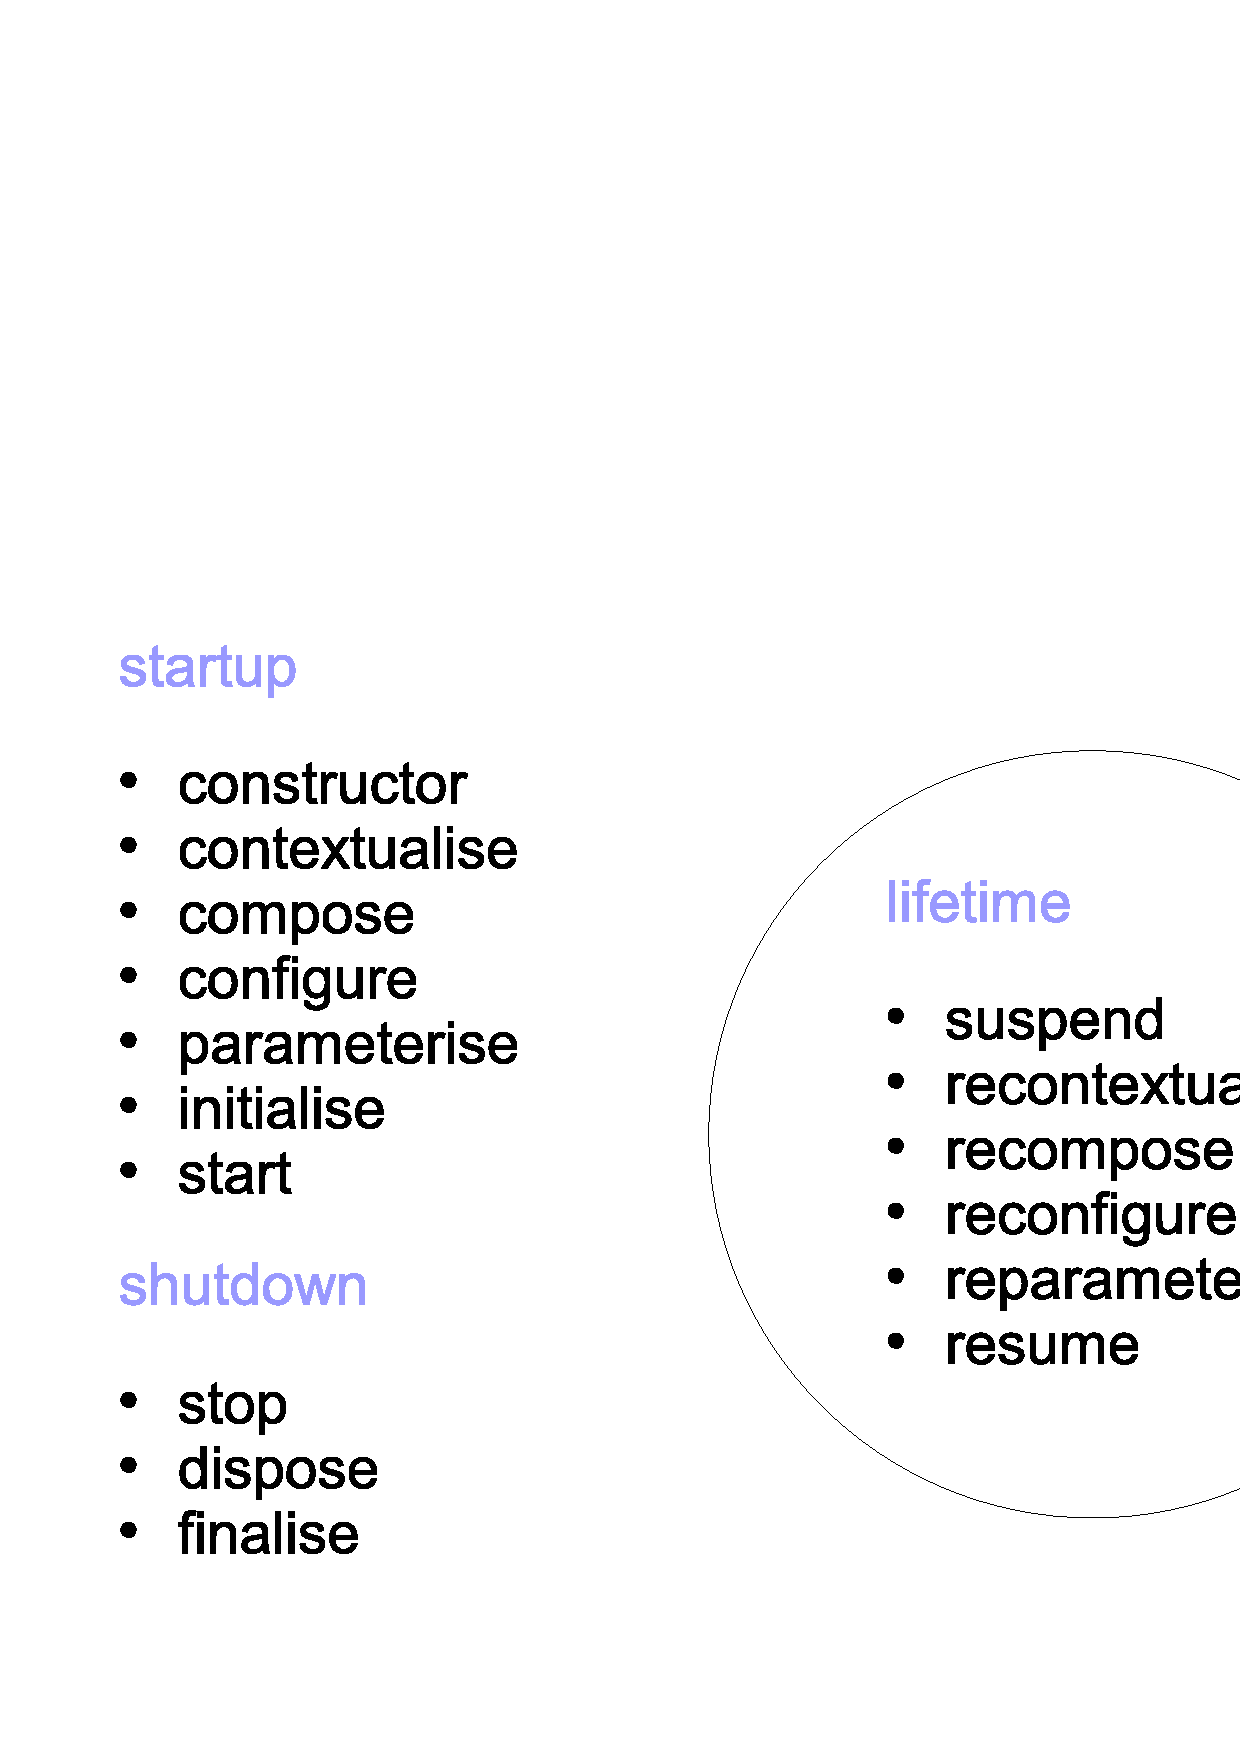
\includegraphics[scale=0.3,angle=-90]{graphic/lifecycle.pdf}
        \caption{Component Lifecycle Methods}
        \label{lifecycle_figure}
    \end{center}
\end{figure}

The lifecycle of a component specifies the methods that can be called on it,
and the order in which this may happen. The corresponding methods are called
\emph{Lifecycle Methods}. Some of them can be called only once in a specific
phase of a component's lifecycle, others may be called multiple times. The
methods in figure \ref{lifecycle_figure} are examples taken from the
\emph{Avalon} \cite{avalon} project. They represent three phases in a
component's lifecycle: \emph{Startup}, \emph{Lifetime} and \emph{Shutdown}.

Lifetime phase methods can be called repeatedly, at various times after startup
and before shutdown. The \emph{constructor} is called as a consequence of
instantiation. Its counterpart \emph{destructor} is not considered in the
project; since \emph{Avalon} is a Java-based framework, it was omitted because a
\emph{Garbage Collector} destroys instances at some indeterminate moment.

\textit{The order in which the various lifecycle methods are called is very
specific. While none are required (it is possible to have a component
implementing none of the lifecycle methods, although the use of that would be
limited), some can only be used when others are as well. It is up to each
container to indicate which lifecycle methods it will honour}, as \cite{avalon}
writes. This should be clearly documented together with the description of the
container.

A component lifecycle allows to forward parameters throughout a whole framework,
which makes static objects such as the singleton managers criticised in section
\ref{global_access_heading} superfluous. The \emph{configure} method, for
example, may forward a \emph{Configuration} object containing parameters that
otherwise would have to be made global.

%
% $RCSfile: interface_and_implementation.tex,v $
%
% Copyright (C) 2002-2008. Christian Heller.
%
% Permission is granted to copy, distribute and/or modify this document
% under the terms of the GNU Free Documentation License, Version 1.1 or
% any later version published by the Free Software Foundation; with no
% Invariant Sections, with no Front-Cover Texts and with no Back-Cover
% Texts. A copy of the license is included in the section entitled
% "GNU Free Documentation License".
%
% http://www.cybop.net
% - Cybernetics Oriented Programming -
%
% http://www.resmedicinae.org
% - Information in Medicine -
%
% Version: $Revision: 1.1 $ $Date: 2008-08-19 20:41:07 $ $Author: christian $
% Authors: Christian Heller <christian.heller@tuxtax.de>
%

\subsection{Interface and Implementation}
\label{interface_and_implementation_heading}
\index{Separation of Interface and Implementation}
\index{Java}
\index{Interface}
\index{Interface Pattern}
\index{Class}
\index{Decoupling of Components}
\index{Java Development Kit}
\index{JDK}

The \emph{Separation of Interface and Implementation} is a core concept of many
programming languages. \emph{Java}, for example, distinguishes \emph{Interface}
and \emph{Class} (section \ref{classification_heading}). Mark Grand's book
\emph{Patterns in Java} \cite{grand} refers to that separation simply as
\emph{Interface} pattern, one of whose uses, after him, were to
\emph{encapsulate components}, that is to:

\begin{itemize}
    \item[-] Force decoupling of different components
    \item[-] Ensure easy changes of interface implementations
    \item[-] Enable users to read interface documentations without having the
        implementation details clutter up their perception
    \item[-] Increase the reuse possibility in larger applications
\end{itemize}

The Java source code example below shows how the \emph{sayHello} method whose
header is declared in the \emph{HelloWorld} interface can be used as
\emph{Application Programming Interface} (API) without knowing anything about
the underlying implementation. Depending on the instance, the method may be
processed on a local or a remote system.

\begin{scriptsize}
    \begin{verbatim}
    package helloworld;
    public interface HelloWorld {
        void sayHello(String greeting);
    }

    package helloworld.impl.default;
    public class DefaultHelloWorld implements HelloWorld {
        void sayHello(String greeting) {
            System.out.println("HelloWorld Greeting: " + greeting);
        }
    }

    package helloworld.impl.remote;
    public class RemoteHelloWorld implements HelloWorld {
        private RemoteMessager remoteMessager;
        public RemoteHelloWorld(RemoteMessager rm) {
            remoteMessager = rm;
        }
        void sayHello(String greeting) {
            rm.sendMessage("HelloWorld Greeting: " + greeting);
        }
    }
    \end{verbatim}
\end{scriptsize}

Further details and recommendations for using interfaces, on examples specific
to the \emph{Java Development Kit} (JDK) \cite{java}, are given in \cite{avalon}.

%
% $RCSfile: separation_of_concerns.tex,v $
%
% Copyright (C) 2002-2008. Christian Heller.
%
% Permission is granted to copy, distribute and/or modify this document
% under the terms of the GNU Free Documentation License, Version 1.1 or
% any later version published by the Free Software Foundation; with no
% Invariant Sections, with no Front-Cover Texts and with no Back-Cover
% Texts. A copy of the license is included in the section entitled
% "GNU Free Documentation License".
%
% http://www.cybop.net
% - Cybernetics Oriented Programming -
%
% http://www.resmedicinae.org
% - Information in Medicine -
%
% Version: $Revision: 1.1 $ $Date: 2008-08-19 20:41:08 $ $Author: christian $
% Authors: Christian Heller <christian.heller@tuxtax.de>
%

\subsection{Separation of Concerns}
\label{separation_of_concerns_heading}
\index{Separation of Concerns}
\index{SoC}
\index{Container}
\index{Component}
\index{Contract}
\index{Separation of Contract and Implementation}
\index{Concern}
\index{Component Oriented Programming}
\index{COP}
\index{Role of a Component}
\index{Electronic Health Record}
\index{EHR}
\index{Service Manager for Components}
\index{Lookup Method identifying Components}
\index{Fully Qualified Name}
\index{FQN}
\index{Component Selector}

The \emph{Avalon} project \cite{avalon} writes:

\begin{quote}
    Separation of concerns in its simplest form is separating a problem into
    different points of view. Every time one uses interfaces within object- or
    component oriented programming, the \emph{Separation of Concerns} (SoC)
    pattern is applied. The interface separates the implementation concern from
    the concern of the user of the interface.
\end{quote}

Interfaces \emph{pool} common methods (section \ref{classification_heading}).
Inheriting an interface, components indicate to their surrounding container
which methods they implement so that the container can use and rely on these.
Therefore, one often talks of a \emph{Contract} between container and
component. The contract defines what the container (as user of the component)
must provide and what the component produces. In the end, the separation of
\emph{Interface and Implementation} (section
\ref{interface_and_implementation_heading}) could be more correctly called
separation of \emph{Contract and Implementation}.

The contract was mentioned in section \ref{component_lifecycle_heading} which
explained that a container is responsible for taking its components through a
lifecycle. The \emph{Avalon} project \cite{avalon} specifies a number of
concerns which enforce the implementation of one or more lifecycle methods.
Here is a list of some concerns referring to the methods of section
\ref{component_lifecycle_heading}:

\begin{itemize}
    \item[-] Loggable
    \item[-] Contextualizable
    \item[-] Composable
    \item[-] Configurable
    \item[-] Initializable
    \item[-] Startable
    \item[-] Suspendable
\end{itemize}

For example, an object that can be configured implements the \emph{Configurable}
interface. The contract surrounding that interface is that the container as
instantiator of the object passes a \emph{Configuration} object to the component
being a configurable object. Just what the configurable object does with the
passed configuration object is irrelevant to the instantiator.

\begin{figure}[ht]
    \begin{center}
        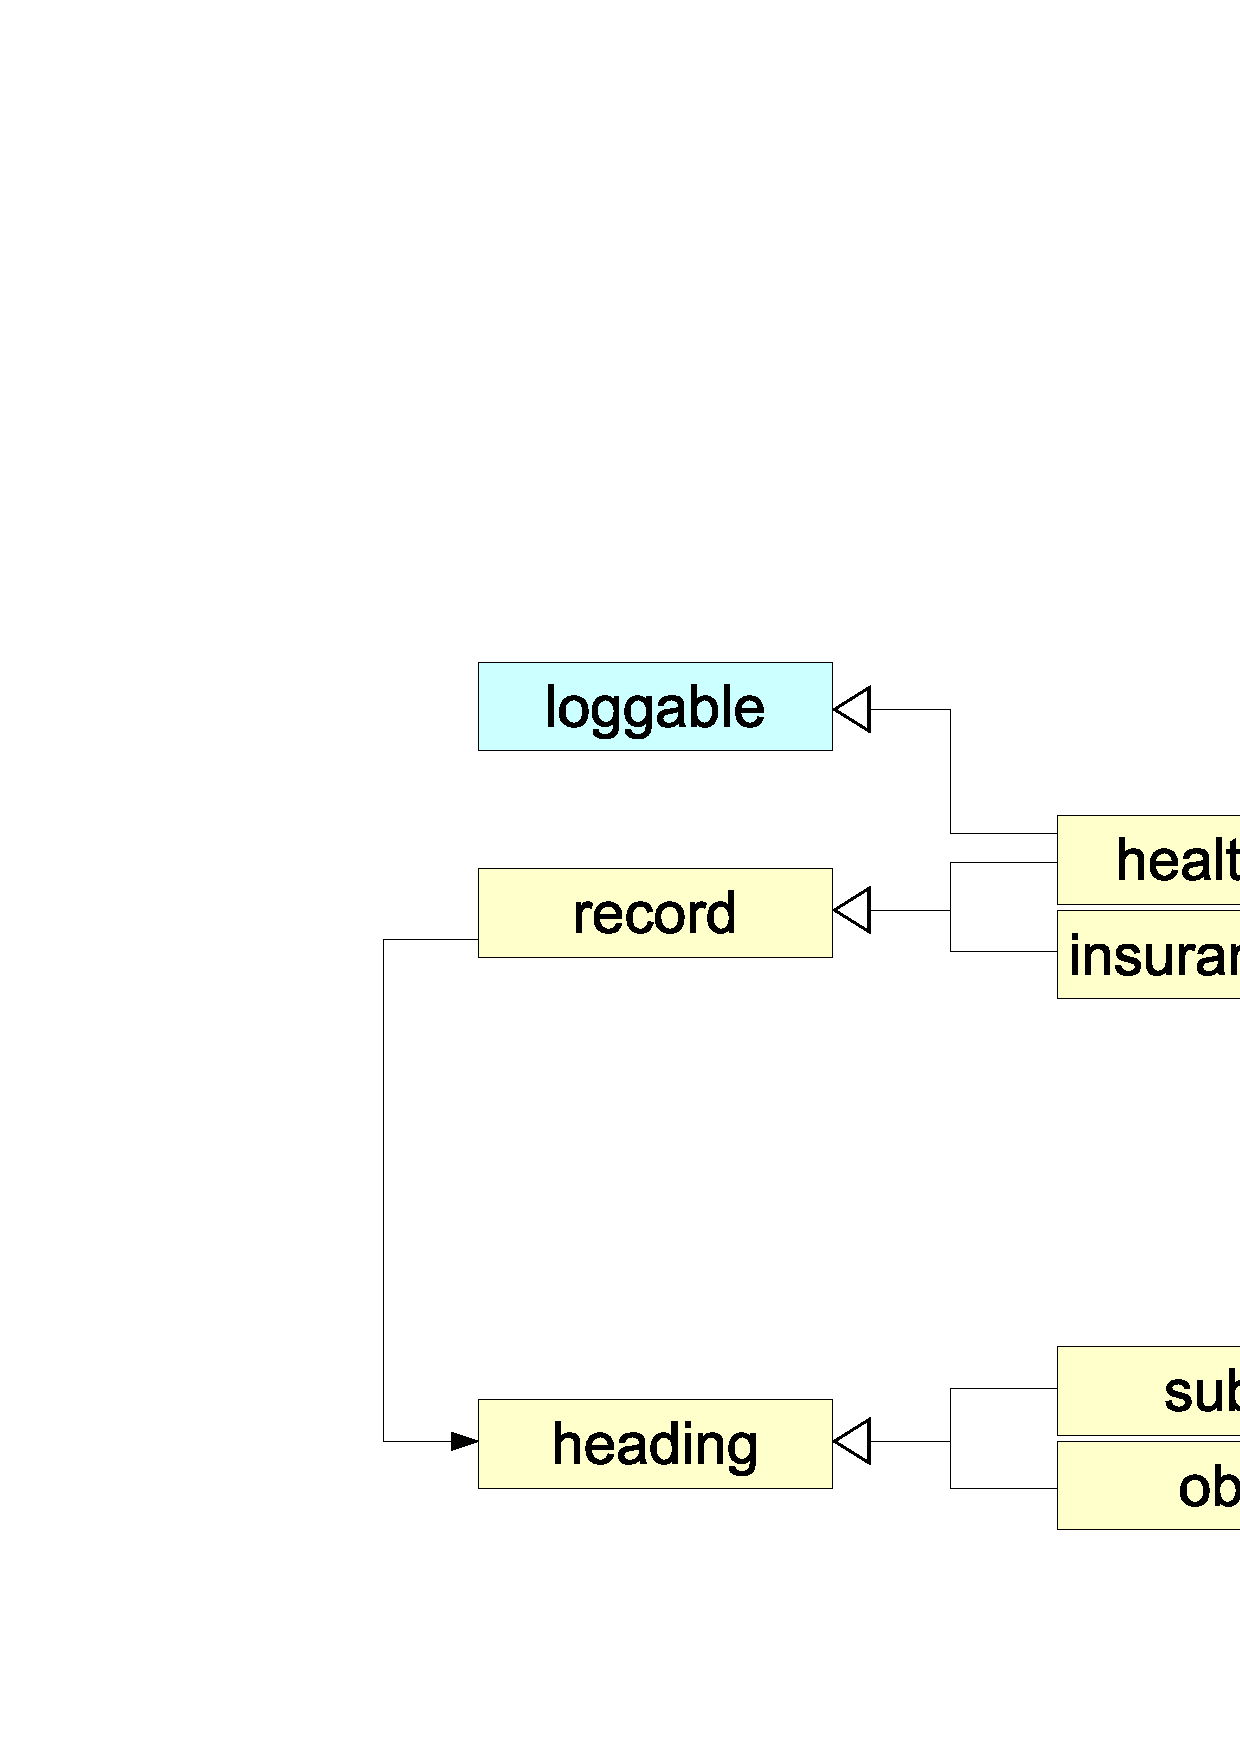
\includegraphics[scale=0.3,angle=-90]{graphic/concern.pdf}
        \caption{Class Inheriting Loggable Concern Interface}
        \label{concern_figure}
    \end{center}
\end{figure}

Figure \ref{concern_figure} shows an \emph{Electronic Health Record} (EHR)
component implementing the \emph{Loggable} interface which indicates that the
component offers functionality for the logging of messages. To fully explain
the figure: The EHR inherits from a general \emph{Record} class that references
so-called \emph{Heading} objects which may be a \emph{Subjective} description
of a patient or an \emph{Objective} result of an examination. Of course, these
objects may be programmed as components as well.

A common comparison used in component oriented programming is that of the
\emph{Role} coming from theater \cite{avalon}. The function or action of a
component's role within a system, as well as its contracts, are defined by its
script -- the interface. Any object that implements the component interface
must comply with the contracts. This allows developers to manipulate components
using a standard interface, without worrying about the semantics of the
implementation. They are separate concerns.

A \emph{Service Manager} is often used to get an instance of the needed
component. The manager's \emph{lookup} method identifies the component based on
the \emph{Fully Qualified Name} (FQN) of the role (interface). If several
components functioning in the same role exist, a \emph{Component Selector} may
be applied to choose the right one. More details are given in \cite{avalon}.

%
% $RCSfile: spread_functionality.tex,v $
%
% Copyright (C) 2002-2008. Christian Heller.
%
% Permission is granted to copy, distribute and/or modify this document
% under the terms of the GNU Free Documentation License, Version 1.1 or
% any later version published by the Free Software Foundation; with no
% Invariant Sections, with no Front-Cover Texts and with no Back-Cover
% Texts. A copy of the license is included in the section entitled
% "GNU Free Documentation License".
%
% http://www.cybop.net
% - Cybernetics Oriented Programming -
%
% http://www.resmedicinae.org
% - Information in Medicine -
%
% Version: $Revision: 1.1 $ $Date: 2008-08-19 20:41:09 $ $Author: christian $
% Authors: Christian Heller <christian.heller@tuxtax.de>
%

\subsection{Spread Functionality}
\label{spread_functionality_heading}
\index{Spread Functionality}
\index{Redundant Code}
\index{Overlapping Code through Concerns}
\index{Spread Functionality through Concerns}
\index{Layer Supertype Pattern}
\index{Lifecycle Method}
\index{Concern-less Development}
\index{Class Hierarchy}
\index{Ontology}

\begin{figure}[ht]
    \begin{center}
        \includegraphics[scale=0.3,angle=-90]{graphic/redundant.pdf}
        \caption{Redundant Code through Usage of Concerns}
        \label{redundant_figure}
    \end{center}
\end{figure}

Separating concerns does not avoid \emph{Redundant Code}. If two independent
components want to target the same concern what they expose by implementing the
corresponding interface, they will both have to implement the required methods
redundantly. This may not be a problem with just two records as in the example
of figure \ref{redundant_figure}, but will become an issue as soon as other
objects are to be programmed as component as well.

Another unwanted effect when using concern interfaces is the \emph{Overlapping}
of concerns (figure \ref{overlapping_figure}). It may happen that a superclass
implements a number of lifecycle methods and their corresponding interfaces
without knowing if its subclasses eventually implement exactly one of these,
too. In such a case, redundant code would appear and the principle of efficient
programming would be injured once more.

\begin{figure}[ht]
    \begin{center}
        \includegraphics[scale=0.3,angle=-90]{graphic/overlapping.pdf}
        \caption{Overlapping Code through Usage of Concerns}
        \label{overlapping_figure}
    \end{center}
\end{figure}

A piece of source code holding a reference to a component instance in form of
a concern interface can \emph{only} call the methods of \emph{that} concern.
Mostly, however, other methods have to be called as well. In this case, a
\emph{Downcast} from the concern interface to the component class implementing
the interface becomes necessary. Yet to be able to downcast, the class (type)
to downcast to needs to be known anyway. In the end, the usability of concern
interfaces turns out to be limited, sometimes even useless, since they only
allow a few methods to be called and information about the real class is not
available.

\begin{figure}[ht]
    \begin{center}
        \includegraphics[scale=0.3,angle=-90]{graphic/spreadbunch.pdf}
        \caption{Concerns Spread Functionality, an Ontology Bunches it}
        \label{spreadbunch_figure}
    \end{center}
\end{figure}

From the viewpoint of reuse, it seems far better to inherit all components from
one common super-class, as suggested by the \emph{Layer Supertype} pattern
(section \ref{layer_supertype_heading}). This class would implement necessary
lifecycle methods just once, being available for all inheriting classes. For the
used example this would mean to eliminate all \emph{Loggable} concern interfaces
(figure \ref{spreadbunch_figure}) and put the logging functionality into the
\emph{Record} super class.

Finally, the only way out of the misery of redundant code caused by concern
interfaces seems to be \emph{Concern-less} software development using
\emph{pure} class hierarchies. And in fact, this is what \emph{Ontologies}
(section \ref{ontology_heading}) are proposing. Section
\ref{separation_of_concerns_heading} mentioned that interfaces help
\emph{pooling} common methods; but in the big system picture, they actually
\emph{spread} them. While concerns represented by interfaces \emph{spread}
functionality, away from the classes that were actually made to \emph{keep} it,
an ontology \emph{bunches} functionality. Chapter \ref{knowledge_schema_heading}
will show some ontology examples and introduce a knowledge schema for their
hierarchical representation, including necessary meta information.

%
% $RCSfile: aspect_oriented_programming.tex,v $
%
% Copyright (C) 2002-2008. Christian Heller.
%
% Permission is granted to copy, distribute and/or modify this document
% under the terms of the GNU Free Documentation License, Version 1.1 or
% any later version published by the Free Software Foundation; with no
% Invariant Sections, with no Front-Cover Texts and with no Back-Cover
% Texts. A copy of the license is included in the section entitled
% "GNU Free Documentation License".
%
% http://www.cybop.net
% - Cybernetics Oriented Programming -
%
% http://www.resmedicinae.org
% - Information in Medicine -
%
% Version: $Revision: 1.1 $ $Date: 2008-08-19 20:41:05 $ $Author: christian $
% Authors: Christian Heller <christian.heller@tuxtax.de>
%

\subsection{Aspect Oriented Programming}
\label{aspect_oriented_programming_heading}
\index{Aspect Oriented Programming}
\index{AOP}
\index{Object Oriented Programming}
\index{OOP}
\index{Concern Interface}
\index{Aspect}
\index{Meta Object Protocol}
\index{MOP}
\index{Mixin Programming Concept}
\index{Crosscutting Concern}
\index{Common Concern}
\index{Aspect Marker Interface}
\index{Component Oriented Programming}
\index{COP}
\index{Development Aspect}
\index{Production Aspect}
\index{Join Point}
\index{Pointcut}
\index{Advice}
\index{Inter-Type Declaration}
\index{Aspect Oriented Software Development}
\index{AOSD}
\index{Aspect Weaver}
\index{Join Point Representation}
\index{Join Point Model}
\index{JPM}
\index{Singleton Pattern}
\index{Lifecycle Method}

Another alternative avoiding redundant code caused by the implementation of
concern interfaces (section \ref{separation_of_concerns_heading}) is the
so-called \emph{Aspect Oriented Programming} (AOP), which is an extension to
\emph{Object Oriented Programming} (OOP). \emph{Aspects} are a possibility to
separate and define concern areas addressed in program code. Wikipedia
\cite{wikipedia} writes that:

\begin{quote}
    Aspects emerged out of object-oriented programming and have functionality
    similar to using a meta-object protocol (section \ref{reflection_heading}).
    Aspects relate closely to programming concepts like subjects, mixins, and
    delegation.
\end{quote}

The Avalon documentation \cite{avalon} means that AOP were: \textit{the next
logical step after separation of concerns}. Many concerns could not be
centrally addressed using the standard mechanisms of programming. Using AOP, it
were possible to do so in a simple fashion.

The AspectJ documentation \cite{aspectj} writes that the motivation for AOP had
been the realisation that there are issues or concerns (like a security policy)
that cut across many of the natural units of modularity of an application and
are not well captured by traditional programming methodologies. For
\emph{Object Oriented Programming} (OOP) languages, the natural unit of
modularity were the \emph{Class}. But in these languages, some concerns were
not easily turned into classes because they'd \emph{cut across} classes. So
these weren't reusable, couldn't be refined or inherited, were spread
throughout the program in an undisciplined way and, in short, were difficult to
work with. AOP were a way of modularising \emph{Crosscutting Concerns} much
like OOP were a way of modularising \emph{Common Concerns}. The later chapter
\ref{statics_and_dynamics_heading} will come back to these two kinds of
concerns in short.

As shown in the previous sections, the \emph{Avalon} project \cite{avalon} uses
concern interfaces (sometimes called \emph{Aspect Marker Interfaces}) and
\emph{Component Oriented Programming} (COP) to define its concerns, what
frequently leads to redundant implementations. Other projects, for instance
\emph{AspectJ} \cite{aspectj} and \emph{AspectWerkz} \cite{aspectwerkz},
provide AOP facilities whose aim is the clean modularisation of crosscutting
concerns such as those in the following list, which AspectJ divides into
\emph{Development Aspects}:

\begin{itemize}
    \item[-] Tracing
    \item[-] Profiling and Logging
    \item[-] Pre- and Post-Conditions
    \item[-] Contract Enforcement
    \item[-] Configuration Management
\end{itemize}

and \emph{Production Aspects}:

\begin{itemize}
    \item[-] Change Monitoring
    \item[-] Context Passing
    \item[-] Providing Consistent Behaviour
\end{itemize}

The AspectJ project as an implementation of AOP for Java adds just one new
concept to that language -- the \emph{Join Point}, which is a well-defined
point in the program flow. A number of new constructs are introduced as well: A
\emph{Pointcut} picks out certain join points and values at those points; an
\emph{Advice} is a piece of code that is executed when a join point is reached.
Both do dynamically affect the program flow. \emph{Inter-Type Declarations}, on
the other hand, statically affect a program's class hierarchy, namely the
members of its classes and the relationships between classes. AspectJ's
\emph{Aspect}, finally, is the unit of modularity for crosscutting concerns. It
behaves somewhat like a Java class, summarising the constructs described
before, that is pointcuts, advices and inter-type declarations.

\emph{Aspect Oriented Software Development} (AOSD) is about developing programs
that rely on AOP principles and languages -- or language extensions,
respectively. Such programs get compiled slightly differently than usual. An
\emph{Aspect Weaver} generates a \emph{Join Point Representation} of the
program, by merging code and aspects. Only afterwards, the program is compiled
into an executable.

Although AOP seems to successfully address the problem of crosscutting concerns,
it also brings with yet another programming paradigm that application developers
have to get familiar with. The new concepts and constructs further complicate
software development. The source code gets further fractured because of AOP's
additional modules. It is harder to follow the program flow and one has less
control on the behaviour of classes, so that the usage of development tools
becomes inevitable. But besides this rather general criticism, there is more
specific ones: The \emph{Join Point Model} (JPM), for example, is reviewed in
\cite{huttenhuis} which points out some unsolved issues in AOP, while
investigating the following properties of join points:

\begin{itemize}
    \item[-] \emph{Granularity:} only some locations in program code are
        suitable as join points
    \item[-] \emph{Encapsulation:} there is no effective way to protect join
        points from aspect-imposed modification
    \item[-] \emph{Semantics:} low-level join point identification leads to
        tight coupling between aspects and join points
    \item[-] \emph{Jumping Aspects:} context-sensitive join points execute
        different aspect code
    \item[-] \emph{Sharing:} dependencies and order of execution are unclear
        when having several pieces of advice at the same join point
\end{itemize}

At least some of the concerns that AOP addresses could be implemented with
lifecycle-techniques as well. A logger, for example, could be created once at
system startup. But instead of accessing it across static methods, as suggested
by the \emph{Singleton} pattern (section \ref{singleton_heading}), or executing
an aspect-oriented \emph{Advice} when a join point is reached, the reference to
the logger instance could simply be forwarded from component to component,
using a special \emph{globalise} lifecycle method, so that each would be able
to access the logger. However, also this solution becomes tedious with a
growing number of objects to be forwarded. The new kind of programming
introduced in part \ref{contribution_heading} of this work therefore suggests
to put general functionality (concerns, aspects) into an interpreter program
acting close to hardware and providing the general functionality to application
systems executed by it.

%
% $RCSfile: agent_oriented_programming.tex,v $
%
% Copyright (C) 2002-2008. Christian Heller.
%
% Permission is granted to copy, distribute and/or modify this document
% under the terms of the GNU Free Documentation License, Version 1.1 or
% any later version published by the Free Software Foundation; with no
% Invariant Sections, with no Front-Cover Texts and with no Back-Cover
% Texts. A copy of the license is included in the section entitled
% "GNU Free Documentation License".
%
% http://www.cybop.net
% - Cybernetics Oriented Programming -
%
% http://www.resmedicinae.org
% - Information in Medicine -
%
% Version: $Revision: 1.1 $ $Date: 2008-08-19 20:41:05 $ $Author: christian $
% Authors: Christian Heller <christian.heller@tuxtax.de>
%

\subsection{Agent Oriented Programming}
\label{agent_oriented_programming_heading}
\index{Agent Oriented Programming}
\index{AGOP}
\index{Component Oriented Programming}
\index{COP}
\index{Inversion of Control Pattern}
\index{IoC}
\index{Application Programming Interface}
\index{API}
\index{Active Component}
\index{Passive Component}
\index{Agent}
\index{Multi Agent System}
\index{MAS}
\index{Agent Communication Language}
\index{ACL}
\index{Language Paradigm}
\index{Ontology}
\index{Mobility of an Agent}
\index{Object Oriented Programming}
\index{OOP}
\index{Speech Act Theory}
\index{Belief of an Agent}
\index{Capability of an Agent}
\index{Decision of an Agent}
\index{Mental State of an Agent}
\index{Knowledge Base of an Agent}
\index{Agent0 Language}

Components created after the principles of \emph{Component Oriented Programming}
(COP) are \emph{passive}, because they follow the \emph{Inversion of Control}
(IoC) pattern. The functionality, or \emph{Service}, they offer is called by a
surrounding container, via a well-defined \emph{Application Programming Interface}
(API). \emph{Active} components, on the other hand, act alone. An \emph{Agent}
is a self-acting component. It runs \emph{autonomically} or
\emph{semi-autonomically}, is \emph{proactive}, \emph{reactive} and
\emph{social} \cite[p. 330]{sowa}. Many individual communicative software
agents may form a \emph{Multi Agent System} (MAS) \cite{wikipedia}.
Communication happens by some \emph{Agent Communication Language} (ACL)
(section \ref{agent_communication_language_heading}). David Parks, who calls
\emph{Agent Oriented Programming} (AGOP) a \emph{Language Paradigm}, writes
\cite{parks}:

\begin{quote}
    In AGOP, objects known as agents interact to achieve individual goals.
    Agents can exist in a structure as complex as a global internet or one as
    simple as a module of a common program. Agents can be autonomous entities,
    deciding their next step without the interference of a user, or they can be
    controllable, serving as a mediary between the user and another agent.
\end{quote}

In search for a uniform definition of the term \emph{Agent}, Ralf Kuehnel
investigated numerous sources of literature but finally comes to the conclusion
\cite[p. 203]{kuehnel} that the term is just a \emph{Metaphor} standing for
different properties, depending on the field it is used in. Typically mentioned
means of agents, however, are \cite[p. 11]{kuehnel}: \emph{Distribution}, common
\emph{Language} and \emph{Ontology} (section \ref{conceptual_network_heading}),
\emph{Cooperation} and \emph{Coordination}, \emph{Security} and \emph{Mobility}.

Comparing \emph{Agents} of AGOP with \emph{Objects} known from OOP, Parks
\cite{parks} writes: \textit{It is not clear, for example, what the concepts of
inheritance and dynamic dispatch mean when discussing an agent.} He points out
the following significant differences:

\begin{itemize}
    \item[-] The fields of an agent are restricted. The state of an agent is
        described in terms of \emph{Beliefs}, \emph{Capabilities} and
        \emph{Decisions} (\emph{Obligation} / \emph{Commitment}). These ideas
        are built into the syntax of the language.
    \item[-] Each message is also defined in terms of mental activities. An agent
        may engage another (or itself) with messaging activities from a restricted
        class of categories. In Shoham's formalism \cite{shoham}, the categories
        of messages are taken from \emph{Speech-Act Theory}; they are:
        \emph{Informing}, \emph{Requesting}, \emph{Offering}, \emph{Accepting},
        \emph{Rejecting}, \emph{Competing} and \emph{Assisting}.
\end{itemize}

Yoav Shoham, who presented AGOP as a new way to describe intelligent agents
\cite{shoham}, suggests that an AGOP system needs three elements to be
complete, a:

\begin{enumerate}
    \item[-] \emph{Formal Language} with clear syntax for describing the mental state
    \item[-] \emph{Programming Language} in which to define agents
    \item[-] \emph{Method} for converting neutral applications into agents
\end{enumerate}

To the \emph{Mental State} of an agent belong information \cite{kuehnel} about its:

\begin{itemize}
    \item[-] \emph{Environment} (constraints)
    \item[-] \emph{Expertise} (capabilities) and \emph{Motivations} (aims)
    \item[-] \emph{Actions} and \emph{Plans}
\end{itemize}

Tim Finin et al. \cite{kqml} classify the statements in a knowledge base into
two categories: \emph{Beliefs} and \emph{Goals}. After them, an agent's beliefs
encoded information it has about itself (capabilities) and its external
environment (constraints), including the knowledge bases of other agents. An
agent's goals encoded states of its external environment that the agent would
act to achieve.

To a running \emph{Agent} system belong the following modules \cite{kuehnel}:

\begin{itemize}
    \item[-] \emph{Knowledge Base:} mental state, as described above
    \item[-] \emph{Controller:} task controller, scheduler and option selection algorithm
    \item[-] \emph{Executor:} task runner and security
    \item[-] \emph{Interaction:} communication handler, sender and receiver
    \item[-] \emph{Management:} lifecycle manager, startup and shutdown
\end{itemize}

While early research in AGOP used special languages like Shoham's \emph{Agent0}
\cite{shoham}, agent-oriented systems created later were also built upon OOP-
and other contemporary programming paradigms \cite[p. 237]{kuehnel}. Ralf
Kuehnel \cite{kuehnel} calls \emph{Agent0} alone a \textit{very limited
programming language} and takes this as evidence for supporting both, the
development of agents and the representation of knowledge with a framework based
on OOP principles. For the implementation of this framework, his choice fell on
Java as system programming language (section \ref{system_programming_heading}).

That is, although AGOP suggests the separation of a system's \emph{Knowledge}
(mental state) from its internal runtime processing and \emph{Control} (agent)
and sees them both as separate elements that should be implemented in
\emph{different} languages (\emph{formal} vs. \emph{programming}), as mentioned
by Shoham (see above), many agent-oriented systems use just \emph{one} language
for implementing both. Even if they are kept in different modules, the conceptual
differences between \emph{high-level} application knowledge and \emph{low-level}
system control cannot be honoured sufficiently. This \emph{Mix-up} puts them on
the same level like traditional systems. \emph{Cybernetics Oriented Programming}
(CYBOP) as described in this work therefore defines a knowledge modelling
language (chapter \ref{cybernetics_oriented_language_heading}) which is
independent from the implementation language of its underlying interpreter.

Furthermore, if OO concepts like \emph{Composition} or \emph{Inheritance} were
present in knowledge models, the usage of an OOP language to implement the actual
agent system could \emph{not} be justified any longer. In such a case, lower-level
\emph{Structured and Procedural Programming} (SPP) languages would suffice, and
work much more efficiently. Chapter \ref{cybernetics_oriented_interpreter_heading}
of this work introduces a knowledge interpreter that is written in the \emph{C}
programming language. The interpreter owns a knowledge base keeping all
application knowledge, and it has modules for lifecycle management, signal
(event) processing, communication etc., just like the definition of an agent
(see above) suggests.


%
% $RCSfile: domain_engineering.tex,v $
%
% Copyright (C) 2002-2008. Christian Heller.
%
% Permission is granted to copy, distribute and/or modify this document
% under the terms of the GNU Free Documentation License, Version 1.1 or
% any later version published by the Free Software Foundation; with no
% Invariant Sections, with no Front-Cover Texts and with no Back-Cover
% Texts. A copy of the license is included in the section entitled
% "GNU Free Documentation License".
%
% http://www.cybop.net
% - Cybernetics Oriented Programming -
%
% http://www.resmedicinae.org
% - Information in Medicine -
%
% Version: $Revision: 1.1 $ $Date: 2008-08-19 20:41:06 $ $Author: christian $
% Authors: Christian Heller <christian.heller@tuxtax.de>
%

\section{Domain Engineering}
\label{domain_engineering_heading}
\index{Domain Engineering}
\index{DE}
\index{Software Engineering Process}
\index{SEP}
\index{Object Oriented Analysis}
\index{OOA}
\index{Object Oriented Design}
\index{OOD}
\index{Six Pack Model}
\index{System Family Engineering}
\index{Application Engineering}
\index{AE}
\index{Analysis Phase}
\index{Design Phase}
\index{Implementation Phase}
\index{Development for Reuse}
\index{Feature Oriented Domain Analysis}
\index{FODA}
\index{Reuse driven Software Engineering Business}
\index{RSEB}
\index{Feature RSEB}
\index{FeatuRSEB}
\index{Unified Modelling Language}
\index{UML}
\index{Feature Model}

Undoubtedly, \emph{Object Oriented Programming} (OOP) (section
\ref{object_oriented_programming_heading}) is one of the most popular programming
paradigms in use today. Its application within a \emph{Software Engineering Process}
(SEP) (chapter \ref{software_engineering_process_heading}) requires two preliminary
phases called \emph{Object Oriented Analysis} (OOA) and \emph{Object Oriented Design}
(OOD).

\begin{figure}[ht]
    \begin{center}
        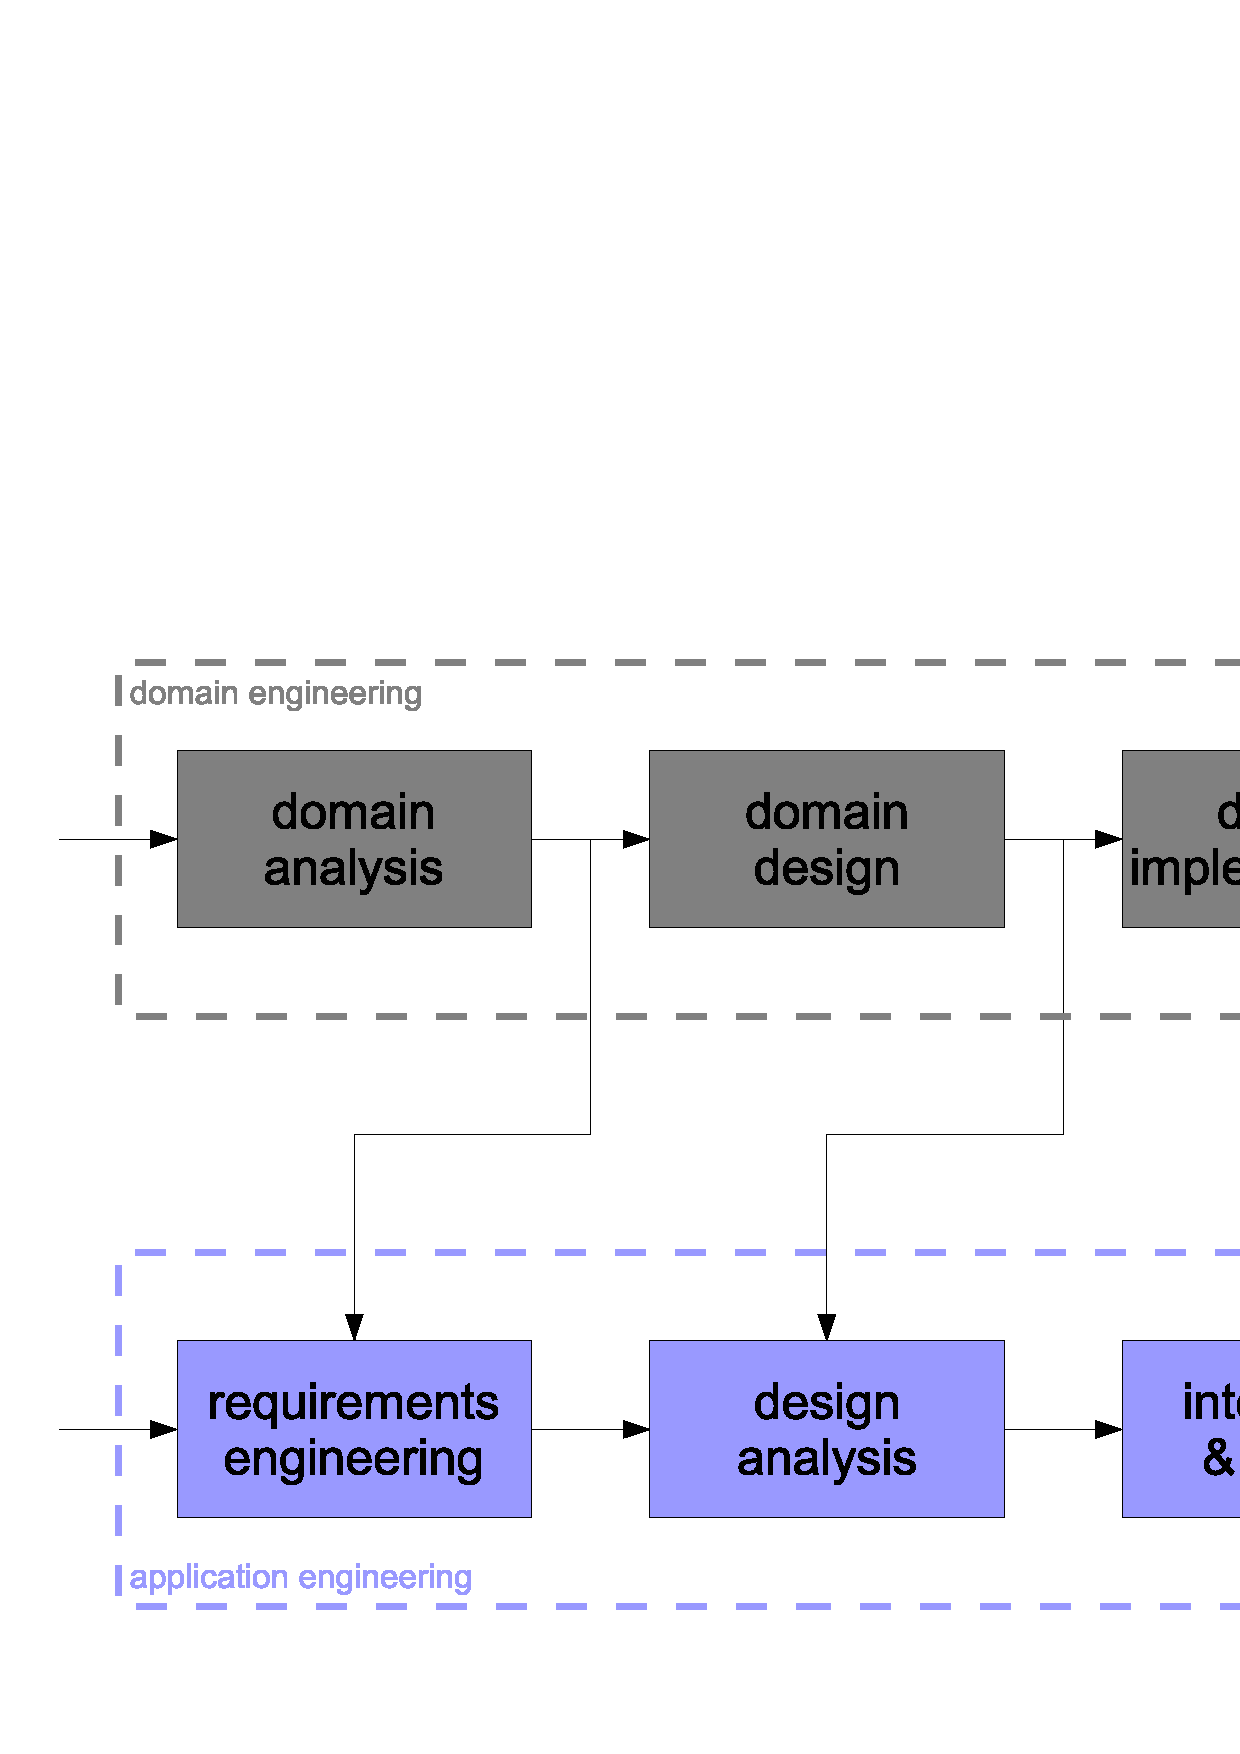
\includegraphics[scale=0.3,angle=-90]{graphic/sixpack.pdf}
        \caption{Six Pack Model of System Family Development \cite{domainengg, esaps}}
        \label{sixpack_figure}
    \end{center}
\end{figure}

The area of \emph{System Family Engineering} applies a so-called \emph{Six-Pack}
approach (figure \ref{sixpack_figure}) which is based on the separation of
\emph{Domain Engineering} (DE) and \emph{Application Engineering} (AE).
\textit{The focus of AE is a single system whereas the focus of DE is on
multiple related systems within a domain}, as \cite{domainengg} defines. Both of
them consist of analysis-, design- and implementation phases. The results of
each DE phase are \emph{fed in} as foundation for the work to be done in AE.
Most of the topics described in the previous sections
(\ref{paradigm_and_language_heading}, \ref{pattern_heading} and
\ref{component_oriented_programming_heading}) turned around techniques which
are applicable to both, DE as well as AE.

In Krzysztof Czarnecki's opinion \cite{czarnecki}, the only SEPs adequately
addressing the issue of \emph{Development for Reuse} were DE methodologies,
most of which had essentially the same structure. He writes:

\begin{quote}
    \emph{Domain Engineering} is the activity of \emph{collecting},
    \emph{organizing}, and \emph{storing} past experience in building systems or
    parts of systems in a particular domain in the form of reusable assets (i.e.
    reusable work-products), as well as providing an adequate means for
    \emph{reusing} these assets (i.e. retrieval, qualification, dissemination,
    adaptation, assembly, etc.) when building new systems.
\end{quote}

After him, the main difference between traditional OOA/ OOD- and DE methods
were that the former focus on developing \emph{Single} systems, the latter
though on developing \emph{Families} of systems. Combined with the definition
stated above (\cite{domainengg}), this means that OOA/ OOD methods may be used
for application-, but not domain engineering. Different methods and techniques
exist for DE. Many are given in \cite{wartik, arrango, fere}. Just a few of
them shall be mentioned here:

\begin{itemize}
    \item{\emph{Feature Oriented Domain Analysis} (FODA)}
    \item{\emph{Reuse driven Software Engineering Business} (RSEB)}
    \item{\emph{Feature RSEB} (FeatuRSEB)}
\end{itemize}

The RSEB methodology \cite{jacobson1997} places emphasis on purely
\emph{Object Oriented} (OO) techniques which it uses together with the
\emph{Unified Modelling Language} (UML). \emph{Features} and \emph{Feature Models}
(section \ref{feature_model_heading}), as concept, were introduced by the FODA
\cite{foda}. The combination of RSEB and FODA results in the FeatuRSEB approach
\cite{griss}. It permits a separate treatment of domain knowledge and system
functionality.

However, this work is less interested in the details of DE software development
\emph{Methods}, but rather in their \emph{Knowledge Abstraction-} and
\emph{Implementation} techniques. Some of them are investigated in the
following sections.

%
% $RCSfile: tool_and_material.tex,v $
%
% Copyright (C) 2002-2008. Christian Heller.
%
% Permission is granted to copy, distribute and/or modify this document
% under the terms of the GNU Free Documentation License, Version 1.1 or
% any later version published by the Free Software Foundation; with no
% Invariant Sections, with no Front-Cover Texts and with no Back-Cover
% Texts. A copy of the license is included in the section entitled
% "GNU Free Documentation License".
%
% http://www.cybop.net
% - Cybernetics Oriented Programming -
%
% http://www.resmedicinae.org
% - Information in Medicine -
%
% Version: $Revision: 1.1 $ $Date: 2008-08-19 20:41:09 $ $Author: christian $
% Authors: Christian Heller <christian.heller@tuxtax.de>
%

\subsection{Tool \& Material}
\label{tool_and_material_heading}
\index{Tools \& Materials Approach}
\index{Domain}
\index{Application}

In software engineering, the term \emph{Domain} stands for a special field of
business in which software systems are applied. Frequently, system development
methods distinguish between data belonging to the \emph{Domain} and
functionality defining the actual \emph{Application} working \emph{on} the
domain. The system family engineering mentioned before is one example.

This view is comparable to the well-known \emph{Tools \& Materials} approach
\cite{tandm} which is based on the distinction of \emph{active} applications
(tools) working on \emph{passive} domain data (material). \textit{Materials can
never be accessed directly, but only by using appropriate tools}, as
\cite{tandm} writes. This simple idea is an important pre-condition for the
separate treatment of \emph{System} and \emph{Knowledge}, as explained in
chapter \ref{statics_and_dynamics_heading} of this work.

%
% $RCSfile: generics.tex,v $
%
% Copyright (C) 2002-2008. Christian Heller.
%
% Permission is granted to copy, distribute and/or modify this document
% under the terms of the GNU Free Documentation License, Version 1.1 or
% any later version published by the Free Software Foundation; with no
% Invariant Sections, with no Front-Cover Texts and with no Back-Cover
% Texts. A copy of the license is included in the section entitled
% "GNU Free Documentation License".
%
% http://www.cybop.net
% - Cybernetics Oriented Programming -
%
% http://www.resmedicinae.org
% - Information in Medicine -
%
% Version: $Revision: 1.1 $ $Date: 2008-08-19 20:41:06 $ $Author: christian $
% Authors: Christian Heller <christian.heller@tuxtax.de>
%

\subsection{Generics}
\label{generics_heading}
\index{Generics}
\index{Generic Programming}
\index{Function Template}
\index{Class Template}
\index{Standard Template Library}
\index{STL}
\index{Eiffel}
\index{Java}
\index{VB.NET}
\index{C\#}
\index{Reuse through Parameterisation}
\index{Dynamic Typing}

\emph{Generic Programming} received its name from the \emph{Generics} it uses.
Wikipedia \cite{wikipedia} writes: \textit{Generics is a technique that allows
one value to take different datatypes (so-called polymorphism) as long as
certain contracts such as subtypes and signature are kept.} \emph{Templates}
are one technique providing generics. They allow the writing of code without
considering the data type that code will eventually be used with. Two kinds of
templates exist \cite{wikipedia}:

\begin{itemize}
    \item[-] \emph{Function Template:} behaving like a function that can accept
        arguments of many different types
    \item[-] \emph{Class Template:} extending the same concept to classes;
        often used to make generic containers
\end{itemize}

Using templates of the C++ \emph{Standard Template Library} (STL) \cite{stl},
a list may be declared by writing \texttt{list<T>}, where \emph{T} represents
the type that may be substituted as needed. A linked list of integers, for
example, would be created with \texttt{list<int>}. After \cite{wikipedia},
there are three primary drawbacks to the use of templates:

\begin{enumerate}
    \item Less portable code due to the poor support for templates in compilers
    \item Difficult development of templates due to unhelpful error messages
        produced by compilers
    \item Bloated code due to the extra code (instantiated template) generated
        by compilers
\end{enumerate}

Meanwhile, many other OOP languages like \emph{Eiffel}, \emph{Java},
\emph{VB.NET} and \emph{C\#} provide generic facilities. Being used to improve
the customisability of code at compile time, they retain the efficiency of
statically configured code. However, in practice (own experience of the author)
it is often hard for programmers to understand and handle generic techniques.
Czarnecki \cite{czarnecki}, who summarises generic programming as \textit{Reuse
through Parameterisation}, criticises that it: \textit{limits code generation
to substituting generic type parameters with concrete types and welding together
pre-existing fragments of code in a fixed pattern.} \emph{Dynamic Typing}
(section \ref{typeless_programming_heading}) is one possibility to circumvent
the need for generic programming. The interpreter program introduced in chapter
\ref{cybernetics_oriented_interpreter_heading} uses dynamic typing; it
references all knowledge via neutral pointers whose meaning gets determined
only at runtime.

%
% $RCSfile: domain_specific_language.tex,v $
%
% Copyright (C) 2002-2008. Christian Heller.
%
% Permission is granted to copy, distribute and/or modify this document
% under the terms of the GNU Free Documentation License, Version 1.1 or
% any later version published by the Free Software Foundation; with no
% Invariant Sections, with no Front-Cover Texts and with no Back-Cover
% Texts. A copy of the license is included in the section entitled
% "GNU Free Documentation License".
%
% http://www.cybop.net
% - Cybernetics Oriented Programming -
%
% http://www.resmedicinae.org
% - Information in Medicine -
%
% Version: $Revision: 1.1 $ $Date: 2008-08-19 20:41:06 $ $Author: christian $
% Authors: Christian Heller <christian.heller@tuxtax.de>
%

\subsection{Domain Specific Language}
\label{domain_specific_language_heading}
\index{Domain Specific Language}
\index{DSL}
\index{General Purpose Language}
\index{GPL}
\index{Little Language}
\index{Application Language}
\index{Macro}
\index{Very High Level Language}
\index{GraphViz DOT}
\index{Mathematica}
\index{Yet Another Compiler Compiler}
\index{YACC}
\index{Universal Interactive Executive}
\index{UNIX}
\index{UNIX Shell Script}
\index{Lisp}
\index{Smalltalk}
\index{In-Language DSL}
\index{C++}
\index{Ruby}

While a \emph{General Purpose Language} (GPL), no matter if in form of a
scripting- or compiled programming language, can be used for performing a
variety of different tasks, a (usually declarative) \emph{Domain Specific Language}
(DSL), though less comprehensive, is more expressive in a special domain
context \cite{deursen}. After \cite{wikipedia}, DSLs may: \textit{enhance the
productivity, reliability, maintainability, portability and reusability of
software.} In Czarnecki's words \cite{czarnecki}, DSLs: \textit{increase the
abstraction level for a particular problem domain} and, being highly
intentional: \textit{allow users to work closely with domain concepts.}

Several synonyms are used to label a DSL, for example: \emph{Little Language},
\emph{Application Language}, \emph{Macro} or \emph{Very High Level Language}
\cite{wikipedia}. To the numerous representatives belong simple spreadsheet
\emph{Macros} as well as graph definition languages like \emph{GraphViz}'s
\emph{DOT} \cite{graphviz}, languages for numerical and symbolic computation as
used in \emph{Mathematica} \cite{mathematica}, or parser generator languages
like \emph{Yet Another Compiler Compiler} (YACC), found on
\emph{Universal Interactive Executive} (UNIX) systems. Even UNIX
\emph{Shell Scripts} can be considered a DSL, with emphasis on data
organisation. Further DSLs exist, yet are the boundaries between the concepts
of domain specific- and other languages quite blurry \cite{wikipedia}.

Martin Fowler \cite{fowlerdsl} mentions that the \emph{Lisp} \cite{commonlisp}
and \emph{Smalltalk} \cite{smalltalk} communities, rather than defining a new
language, frequently morph the GPL into a DSL, in a \emph{bottom-up} manner.
Such \emph{In-Language} DSLs, as he calls them, use constructs of the
programming language itself. Wondering why, programming in Smalltalk, he never
really felt the need to use a separate language, while, programming in C++/
Java/ C\#, quite often he did, he concludes \cite{fowlerdsl} that: \textit{the
more suitable languages (are) minimalist ones with a single basic idea that's
deeper and simpler than traditional languages (function application for lisp,
objects and messages for smalltalk)}, and finds that it is the
\textit{friendliness towards in-language DSLs} rather than \textit{static
versus dynamic typing} that let many software developers \textit{enjoy
programming in Smalltalk or Ruby so much more than in Java or C\#}.

Besides their limited usability outside the special domain they were created
for, to the problems that the usage of DSLs brings with belong after
\cite{menzies}:

\begin{itemize}
    \item[-] High cost of designing, implementing, and maintaining a DSL
    \item[-] Difficult finding of the proper scope
    \item[-] Difficult balancing between domain-specificity and GPL constructs
    \item[-] Potential loss of efficiency when compared with hand-coded software
\end{itemize}

The language introduced in chapter \ref{cybernetics_oriented_language_heading}
is simple and just because of that flexible enough to be applicable for
modelling the knowledge of arbitrary domains. It might have the potential to
replace some of the existing DSLs, the investigation of what is out of the
scope of this work, though.

%
% $RCSfile: specification_language.tex,v $
%
% Copyright (C) 2002-2008. Christian Heller.
%
% Permission is granted to copy, distribute and/or modify this document
% under the terms of the GNU Free Documentation License, Version 1.1 or
% any later version published by the Free Software Foundation; with no
% Invariant Sections, with no Front-Cover Texts and with no Back-Cover
% Texts. A copy of the license is included in the section entitled
% "GNU Free Documentation License".
%
% http://www.cybop.net
% - Cybernetics Oriented Programming -
%
% http://www.resmedicinae.org
% - Information in Medicine -
%
% Version: $Revision: 1.1 $ $Date: 2008-08-19 20:41:09 $ $Author: christian $
% Authors: Christian Heller <christian.heller@tuxtax.de>
%

\subsection{Specification Language}
\label{specification_language_heading}
\index{Specification Language}
\index{Unified Modeling Language}
\index{UML}
\index{Feature Model}
\index{Z Specification Language}
\index{B Specification Language}
\index{Vienna Development Method - Specification Language}
\index{VDM-SL}
\index{Specification and Description Language}
\index{SDL}
\index{Extended Meta Language}
\index{Extended ML}

A \emph{Specification Language}, after \cite{wikipedia}, were a formal language
used during system analysis and design, as opposed to a \emph{Programming Language},
which were a mostly directly executable formal language used to implement a system.
As its name already indicates, a specification language describes systems at a much
higher abstract level than a programming language does. But that also means that it:
\textit{must be subject to a process of refinement (the filling-in of implementation
detail), before it can actually be implemented}, as \cite{wikipedia} writes.

Many kinds of specification languages exist. Being a de facto standard, only
the first two of those representatives listed following are introduced in
slightly more detail below:

\begin{itemize}
    \item[-] \emph{Unified Modeling Language} (UML) \cite{uml}
    \item[-] \emph{Feature Model} \cite{foda}
    \item[-] \emph{Z Specification Language} \cite{zspeclang} and
        \emph{B Specification Language} \cite{zb2005}
    \item[-] \emph{Vienna Development Method - Specification Language} (VDM-SL) \cite{vdmsl}
    \item[-] \emph{Specification and Description Language} (SDL) \cite{sdl}
    \item[-] \emph{Extended Meta Language} (Extended ML) \cite{extendedml}
\end{itemize}

%
% $RCSfile: unified_modeling_language.tex,v $
%
% Copyright (C) 2002-2008. Christian Heller.
%
% Permission is granted to copy, distribute and/or modify this document
% under the terms of the GNU Free Documentation License, Version 1.1 or
% any later version published by the Free Software Foundation; with no
% Invariant Sections, with no Front-Cover Texts and with no Back-Cover
% Texts. A copy of the license is included in the section entitled
% "GNU Free Documentation License".
%
% http://www.cybop.net
% - Cybernetics Oriented Programming -
%
% http://www.resmedicinae.org
% - Information in Medicine -
%
% Version: $Revision: 1.1 $ $Date: 2008-08-19 20:41:09 $ $Author: christian $
% Authors: Christian Heller <christian.heller@tuxtax.de>
%

\subsubsection{Unified Modeling Language}
\label{unified_modeling_language_heading}
\index{Unified Modeling Language}
\index{UML}
\index{Class Diagram}
\index{Activity Diagram}
\index{Sequence Diagram}
\index{Use Case Diagram}
\index{State Machine Diagram}
\index{State Chart Diagram}
\index{Component Diagram}
\index{Deployment Diagram}
\index{Object Diagram}
\index{Instance Diagram}
\index{Package Diagram}
\index{Communication Diagram}
\index{Collaboration Diagram}
\index{Composite Structure Diagram}
\index{Interaction Overview Diagram}
\index{Timing Diagram}
\index{UML Diagram Type}
\index{Object Constraint Language}
\index{OCL}
\index{Structure Diagram}
\index{Behaviour Diagram}
\index{Interaction Diagram}
\index{Functional Model}
\index{Object Model}
\index{Dynamic Model}
\index{UML Tool}
\index{Computer Aided Software Engineering Tool}
\index{CASE Tool}
\index{Object Process Diagram}
\index{OPD}
\index{Entity Relationship Diagram}
\index{ERD}

Meanwhile, the probably most famous modelling- and specification language is
the \emph{Unified Modeling Language} (UML) \cite{uml, booch}. It uses a
graphical notation defining a number of diagrams. UML 2.x specifications
\cite{uml} extend the number of different diagram types from 9 (UML 1.x) to 13.
A good overview is given by Ambler in \cite{ambler2005}, which table
\ref{diagrams_table} reproduces in adapted form, showing only \emph{some}
diagram elements. The column \emph{Importance} contains a certainly subjective
recommendation of Ambler, indicating the \emph{Learning Priority} the single
diagram types have in his opinion (which the author of this work supports).

\begin{table}[ht]
    \begin{center}
        \begin{footnotesize}
        \begin{tabular}{| p{35mm} | p{55mm} | p{15mm} |}
            \hline
            \textbf{Diagram} & \textbf{Elements} & \textbf{Importance}\\
            \hline
            Class (CsD) & Class, Inheritance, Association & High\\
            \hline
            Activity (AD) & Activity, Flow, Fork/ Join, Condition, Decision/ Merge & High\\
            \hline
            Sequence (SD) & Object, Lifeline, Activation Box (Method-Invocation Box), Message & High\\
            \hline
            Use Case (UCD) & Use Case, Actor, Association & Medium\\
            \hline
            State Machine (SMD), formerly State Chart Diagram & State, Transition & Medium\\
            \hline
            Component (CmD) & Component, Interface, Dependency & Medium\\
            \hline
            Deployment (DD) & Node, Connection & Medium\\
            \hline
            Object (ObD), also referred to as Instance Diagram & Object, Relationship & Low\\
            \hline
            Package (PD) & Package, Dependency & Low\\
            \hline
            Communication (CoD), formerly Collaboration Diagram & Object, Association & Low\\
            \hline
            Composite Structure (CSD) & Collaboration, Object, Role & Low\\
            \hline
            Interaction Overview (IOD) & Interaction Frame, Interaction Occurrence Frame & Low\\
            \hline
            Timing (TiD) & Object, Lifeline, State, Timing Constraint & Low\\
            \hline
        \end{tabular}
        \end{footnotesize}
        \caption{UML 2.x Diagram Types \cite{ambler2005}}
        \label{diagrams_table}
    \end{center}
\end{table}

One extension to the UML that is now also part of the corresponding de-facto
standard, is the \emph{Object Constraint Language} (OCL). Being a declarative
language, it describes rules applying to UML models, in a precise text format.
This is because not all rules can be expressed by diagrammatic notation
\cite{wikipedia}. The range of possible rules comprises constraints like pre-
and post-conditions or object query expressions. \cite{ocl}

A common classification distinguishes UML diagrams as follows \cite{ambler2005}:

\begin{enumerate}
    \item \emph{Structure:} CsD, CmD, CSD, DD, ObD, PD
    \item \emph{Behaviour:} AD, SMD, UCD
    \item \emph{Interaction:} CoD, IOD, SD, TiD
\end{enumerate}

Others share the information represented by the diagrams according to an
underlying, independently existing model \cite{wikipedia}:

\begin{itemize}
    \item[-] \emph{Functional Model} (UCD): Functionality of the system from
        the user's point of view
    \item[-] \emph{Object Model} (CsD): Structure and substructure of the
        system using objects, attributes, operations, and associations
    \item[-] \emph{Dynamic Model} (AD, SD, SCD): Internal behaviour of the
        system
\end{itemize}

A program working with UML diagrams is called \emph{UML Tool}, or more exactly
\emph{Computer Aided Software Engineering} (CASE) tool. Many of these programs
have developed and matured, over the past decade of years. Besides the standard
UML diagram types, they offer source code parsing and -generation,
documentation creation and more. Some tools introduced their own extensions to
the UML de-facto standard, for example: \emph{Object Process Diagram} (OPD)
\cite{burkhardt} and \emph{Entity Relationship Diagram} (ERD) \cite{otw}. The
description of a hypothetic design tool suggested for the language being
introduced in chapter \ref{cybernetics_oriented_language_heading} will refer
back to the UML diagrams as mentioned in this section, and suggest a different
way to categorise them. Further, chapter \ref{cybernetics_oriented_language_heading}
will try to define four diagram types to be used in conjunction with the
language described in it.

%
% $RCSfile: feature_model.tex,v $
%
% Copyright (C) 2002-2008. Christian Heller.
%
% Permission is granted to copy, distribute and/or modify this document
% under the terms of the GNU Free Documentation License, Version 1.1 or
% any later version published by the Free Software Foundation; with no
% Invariant Sections, with no Front-Cover Texts and with no Back-Cover
% Texts. A copy of the license is included in the section entitled
% "GNU Free Documentation License".
%
% http://www.cybop.net
% - Cybernetics Oriented Programming -
%
% http://www.resmedicinae.org
% - Information in Medicine -
%
% Version: $Revision: 1.1 $ $Date: 2008-08-19 20:41:06 $ $Author: christian $
% Authors: Christian Heller <christian.heller@tuxtax.de>
%

\subsubsection{Feature Model}
\label{feature_model_heading}
\index{Feature Model}
\index{Feature Modelling}
\index{System Family}
\index{Software Product Line}
\index{Feature Driven Design}
\index{Software Engineering Process}
\index{SEP}
\index{Feature Oriented Domain Analysis}
\index{FODA}
\index{Traceability}

Czarnecki \cite{czarnecki} sees \emph{Feature Modelling}, a technique for
analysing and capturing \emph{common} and \emph{variable} features of a family
of systems as well as their inter-dependencies in form of a \emph{Feature Model},
as the main contribution of domain engineering to OOA/ OOD methods. The
\emph{System Families}, also called \emph{Software Product Lines}, whose
development feature models shall support, are described by Kai Boellert
\cite{boellert} as \textit{group of software systems that are developed from a
common set of reusable components}. Czarnecki writes:

\begin{quote}
    \emph{Feature Models} represent the configurability aspect of reusable
    software at an abstract level, i.e. without committing to any particular
    implementation technique such as inheritance, aggregation, or parameterized
    classes. Developers construct the initial models of the reusable software
    in the form of feature models and use them to \emph{guide} the design and
    implementation (also called \emph{Feature-driven Design}). To a reuser, on
    the other hand, feature models represent an \emph{overview} of the
    functionality of the reusable software and a guide to \emph{configuring} it
    for a specific usage context.
\end{quote}

\begin{figure}[ht]
    \begin{center}
        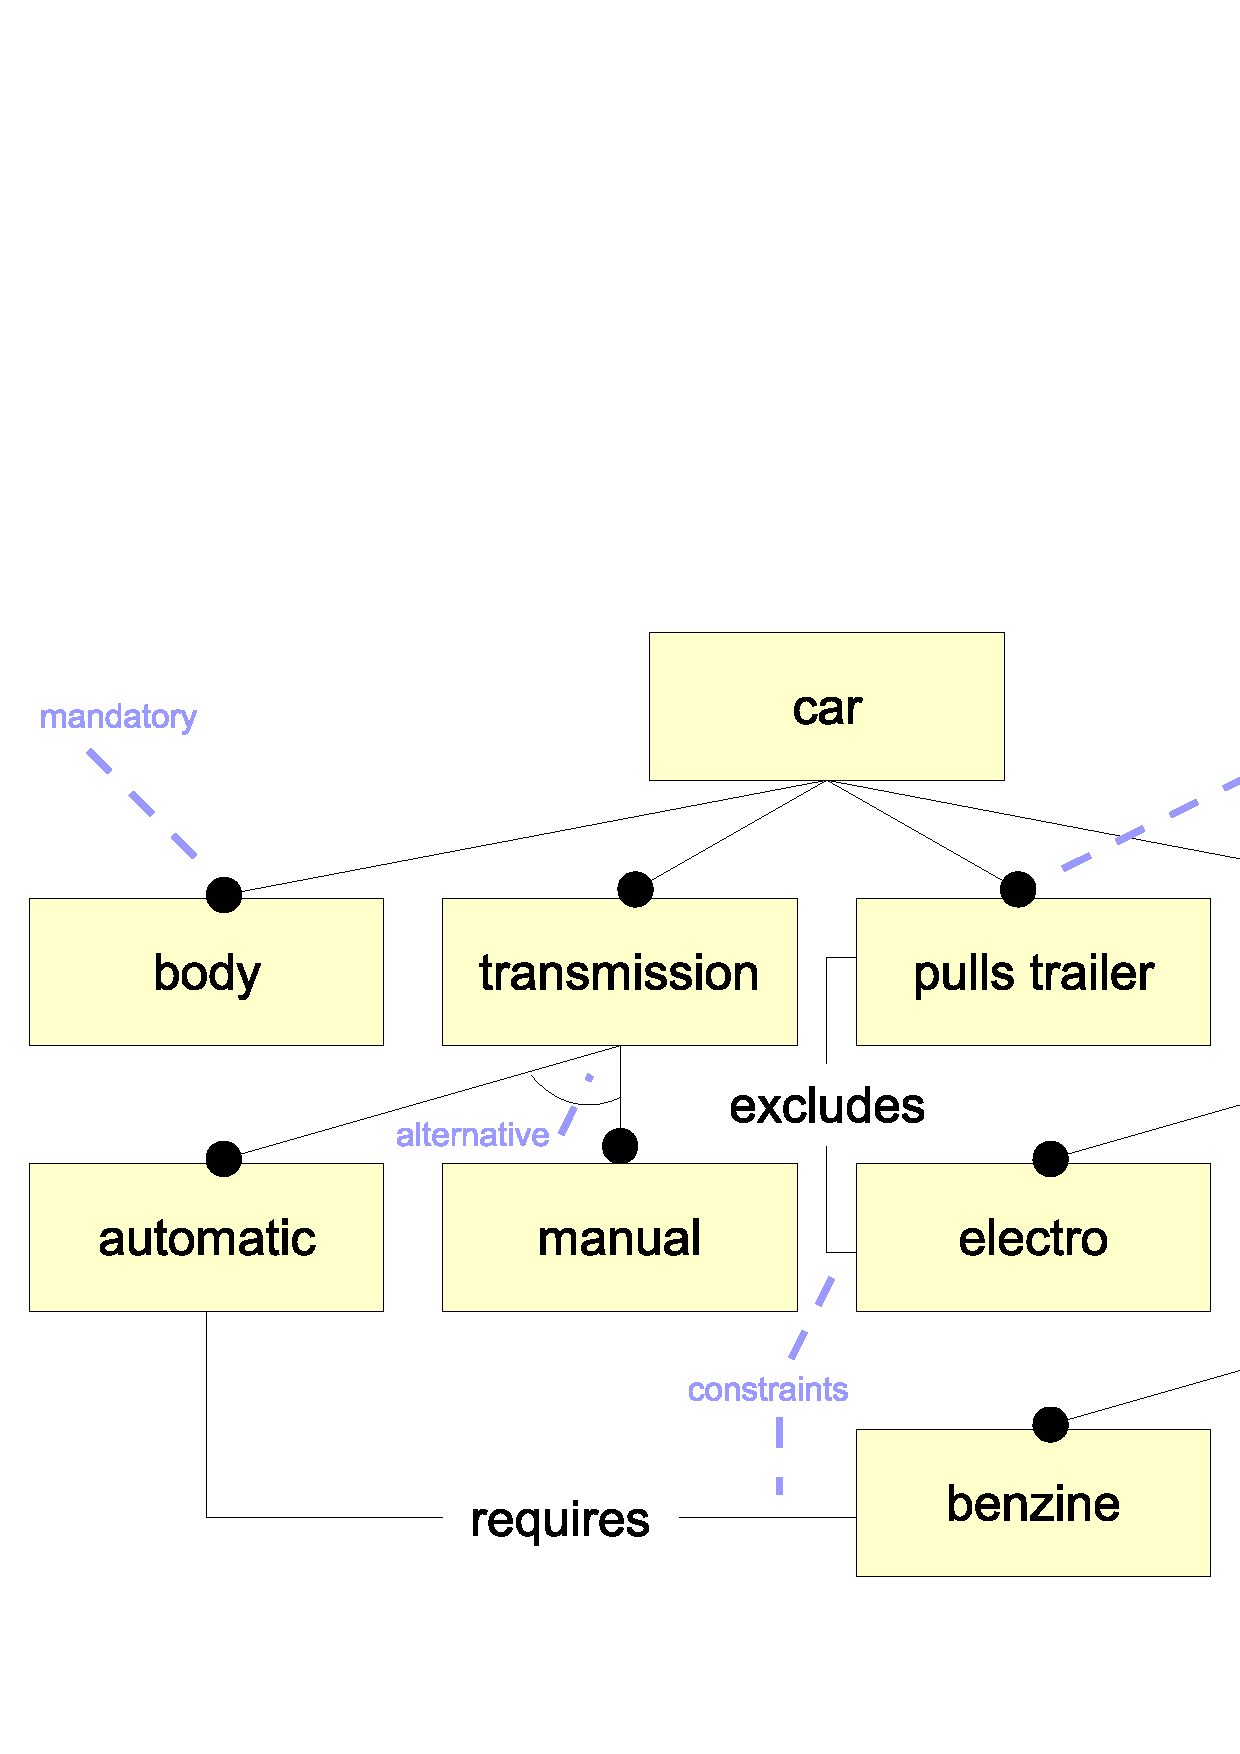
\includegraphics[scale=0.3,angle=-90]{graphic/feature.pdf}
        \caption{Classical Feature Model Diagram of a Car (based on \cite{pashov})}
        \label{feature_figure}
    \end{center}
\end{figure}

In other words, a feature model (figure \ref{feature_figure}) is an additional
form of abstraction within a \emph{Software Engineering Process} (SEP), placed
between analysis- and design models. The properties contained in a feature model
are structured hierarchically. In the \emph{Feature Oriented Domain Analysis}
(FODA) \cite{foda}, a feature model distinguishes three kinds of features:
\emph{Context}, \emph{Representation}, \emph{Operational}. Detlef Streitferdt
\cite{streitferdt200412} defines five feature types:

\begin{enumerate}
    \item \emph{Functional:} used by customer to compose a system
    \item \emph{Interface:} describe required and provided component interfaces
    \item \emph{Parameter:} used to configure functional features
    \item \emph{Structural:} relevant for an automated choice of components
    \item \emph{Conditional:} summarise sub-features to improve readability
\end{enumerate}

Using feature models, the \emph{Traceability} between concrete requirements and
architecture components can be improved. Requirements can better be mapped to
architecture elements, so that also the \emph{Communication} between
stakeholders in the development process can profit. The big abstraction gap
(number \emph{1} in figure \ref{gaps_figure} of section
\ref{abstraction_gaps_heading}) gets split into two smaller (\emph{1a} and
\emph{1b} in figure \ref{gaps_figure}) that do not close the gap conclusively,
but make it easier to cross. The disadvantage of using feature models in a SEP,
however, is that another abstraction gap causing additional effort is created
through them.

The knowledge schema and language introduced in chapters
\ref{knowledge_schema_heading} and \ref{cybernetics_oriented_language_heading}
use a hierarchical structure comparable to the feature model. Their elements,
though, do belong to just one of two possible kinds: \emph{whole-part} model or
\emph{meta property} model. CYBOP knowledge models merge \emph{some} of the
information that would traditionally be found in feature models with that
contained in the design diagrams and might thus be able to eliminate gap 1b.
Non-functional requirements like \emph{Performance}, \emph{Scalability},
\emph{Usability} or \emph{Memory Efficiency} are \emph{not} part of a CYBOP
knowledge model, since they have nothing to do with the actual modelling of
real-world items in form of abstract concepts and belong into a corresponding
analysis- and specification document only.


%
% $RCSfile: generative_programming.tex,v $
%
% Copyright (C) 2002-2008. Christian Heller.
%
% Permission is granted to copy, distribute and/or modify this document
% under the terms of the GNU Free Documentation License, Version 1.1 or
% any later version published by the Free Software Foundation; with no
% Invariant Sections, with no Front-Cover Texts and with no Back-Cover
% Texts. A copy of the license is included in the section entitled
% "GNU Free Documentation License".
%
% http://www.cybop.net
% - Cybernetics Oriented Programming -
%
% http://www.resmedicinae.org
% - Information in Medicine -
%
% Version: $Revision: 1.1 $ $Date: 2008-08-19 20:41:06 $ $Author: christian $
% Authors: Christian Heller <christian.heller@tuxtax.de>
%

\subsection{Generative Programming}
\label{generative_programming_heading}
\index{Generative Programming}
\index{GP}
\index{Aspect Oriented Programming}
\index{AOP}
\index{Generic Programming}
\index{Domain Specific Language}
\index{DSL}
\index{Feature Model}
\index{Generator}
\index{Model Driven Architecture}
\index{MDA}

\emph{Generative Programming} (GP), as proposed by Czarnecki \cite{czarnecki},
is \textit{a comprehensive software development paradigm to achieving high
intentionality, reusability, and adaptability without the need to compromise
the runtime performance and computing resources of the produced software.} It
encompasses techniques of the following, previously described paradigms:

\begin{itemize}
    \item[-] \emph{Aspect Oriented Programming} (AOP) (section
        \ref{aspect_oriented_programming_heading}): used to achieve separation
        of concerns
    \item[-] \emph{Generic Programming} (section \ref{generics_heading}): used
        to parameterise over types
    \item[-] \emph{Domain Specific Language} (DSL) (section
        \ref{domain_specific_language_heading}): used to improve
        intentionality, optimisation and error checking of program code
    \item[-] \emph{Feature Model} (section \ref{feature_model_heading}): used
        as configuration knowledge, to map between problem- and solution space
\end{itemize}

Czarnecki's work contributes to the formal specification and extension of the
\emph{Feature Model}, but does not itself deliver new forms of knowledge
abstraction. GP, however, is mentioned here because of its idea of applying
\emph{Generators} (or generative techniques) producing implementation source
code for a software system from the higher-level specifications defined in the
design phase. Similar techniques are used in the
\emph{Model Driven Architecture} (see next section). GP is a trial to automate
the process of crossing abstraction gap number \emph{2} (with reference to
figure \ref{gaps_figure}), and it is often quite successful. However, the gap
between architecture design models and program source code remains. Chapter
\ref{knowledge_schema_heading} will introduce a \emph{Knowledge Schema} serving
as universal type, so that differing type-based architectures do not have to be
designed anymore.

%
% $RCSfile: model_driven_architecture.tex,v $
%
% Copyright (C) 2002-2008. Christian Heller.
%
% Permission is granted to copy, distribute and/or modify this document
% under the terms of the GNU Free Documentation License, Version 1.1 or
% any later version published by the Free Software Foundation; with no
% Invariant Sections, with no Front-Cover Texts and with no Back-Cover
% Texts. A copy of the license is included in the section entitled
% "GNU Free Documentation License".
%
% http://www.cybop.net
% - Cybernetics Oriented Programming -
%
% http://www.resmedicinae.org
% - Information in Medicine -
%
% Version: $Revision: 1.1 $ $Date: 2008-08-19 20:41:07 $ $Author: christian $
% Authors: Christian Heller <christian.heller@tuxtax.de>
%

\subsection{Model Driven Architecture}
\label{model_driven_architecture_heading}
\index{Model Driven Architecture}
\index{MDA}
\index{Object Management Group}
\index{OMG}
\index{Unified Modeling Language}
\index{UML}
\index{Meta Object Facility}
\index{MOF}
\index{Interface Definition Language}
\index{IDL}
\index{XML Metadata Interchange}
\index{XMI}
\index{Extensible Markup Language}
\index{XML}
\index{Common Warehouse Metamodel}
\index{CWM}
\index{Common Object Request Broker Architecture}
\index{CORBA}
\index{Platform Independent Model}
\index{PIM}
\index{Platform Specific Model}
\index{PSM}
\index{Computer Aided Software Engineering Tool}
\index{CASE Tool}
\index{DE}
\index{DE}
\index{DE}
\index{DE}

The \emph{Model Driven Architecture} (MDA) \cite{mda} (figure \ref{mda_figure}),
an approach to application design and implementation \cite{brown2004} specified
by the \emph{Object Management Group} (OMG), represents a suite of key
standards including:

\begin{itemize}
    \item[-] \emph{Unified Modeling Language} (UML): modelling, visualising and
        documenting the structure and behaviour of systems using graphical
        diagrams
    \item[-] \emph{Meta Object Facility} (MOF): representing and manipulating
        meta models using CORBA and its \emph{Interface Definition Language}
        (IDL); UML can be expressed in terms of MOF, which is done to generate
        XMI
    \item[-] \emph{XML Metadata Interchange} (XMI): interchanging UML
        metamodels and models using an \emph{Extensible Markup Language}
        (XML)-based format
    \item[-] \emph{Common Warehouse Metamodel} (CWM): enabling data mining
        across database boundaries at an enterprise using a complete,
        comprehensive metamodel; does for data modelling what UML does for
        application modelling
    \item[-] \emph{Common Object Request Broker Architecture} (CORBA):
        communicating using a programming language-, operating system- and
        vendor-independent middleware platform
\end{itemize}

\begin{figure}[ht]
    \begin{center}
        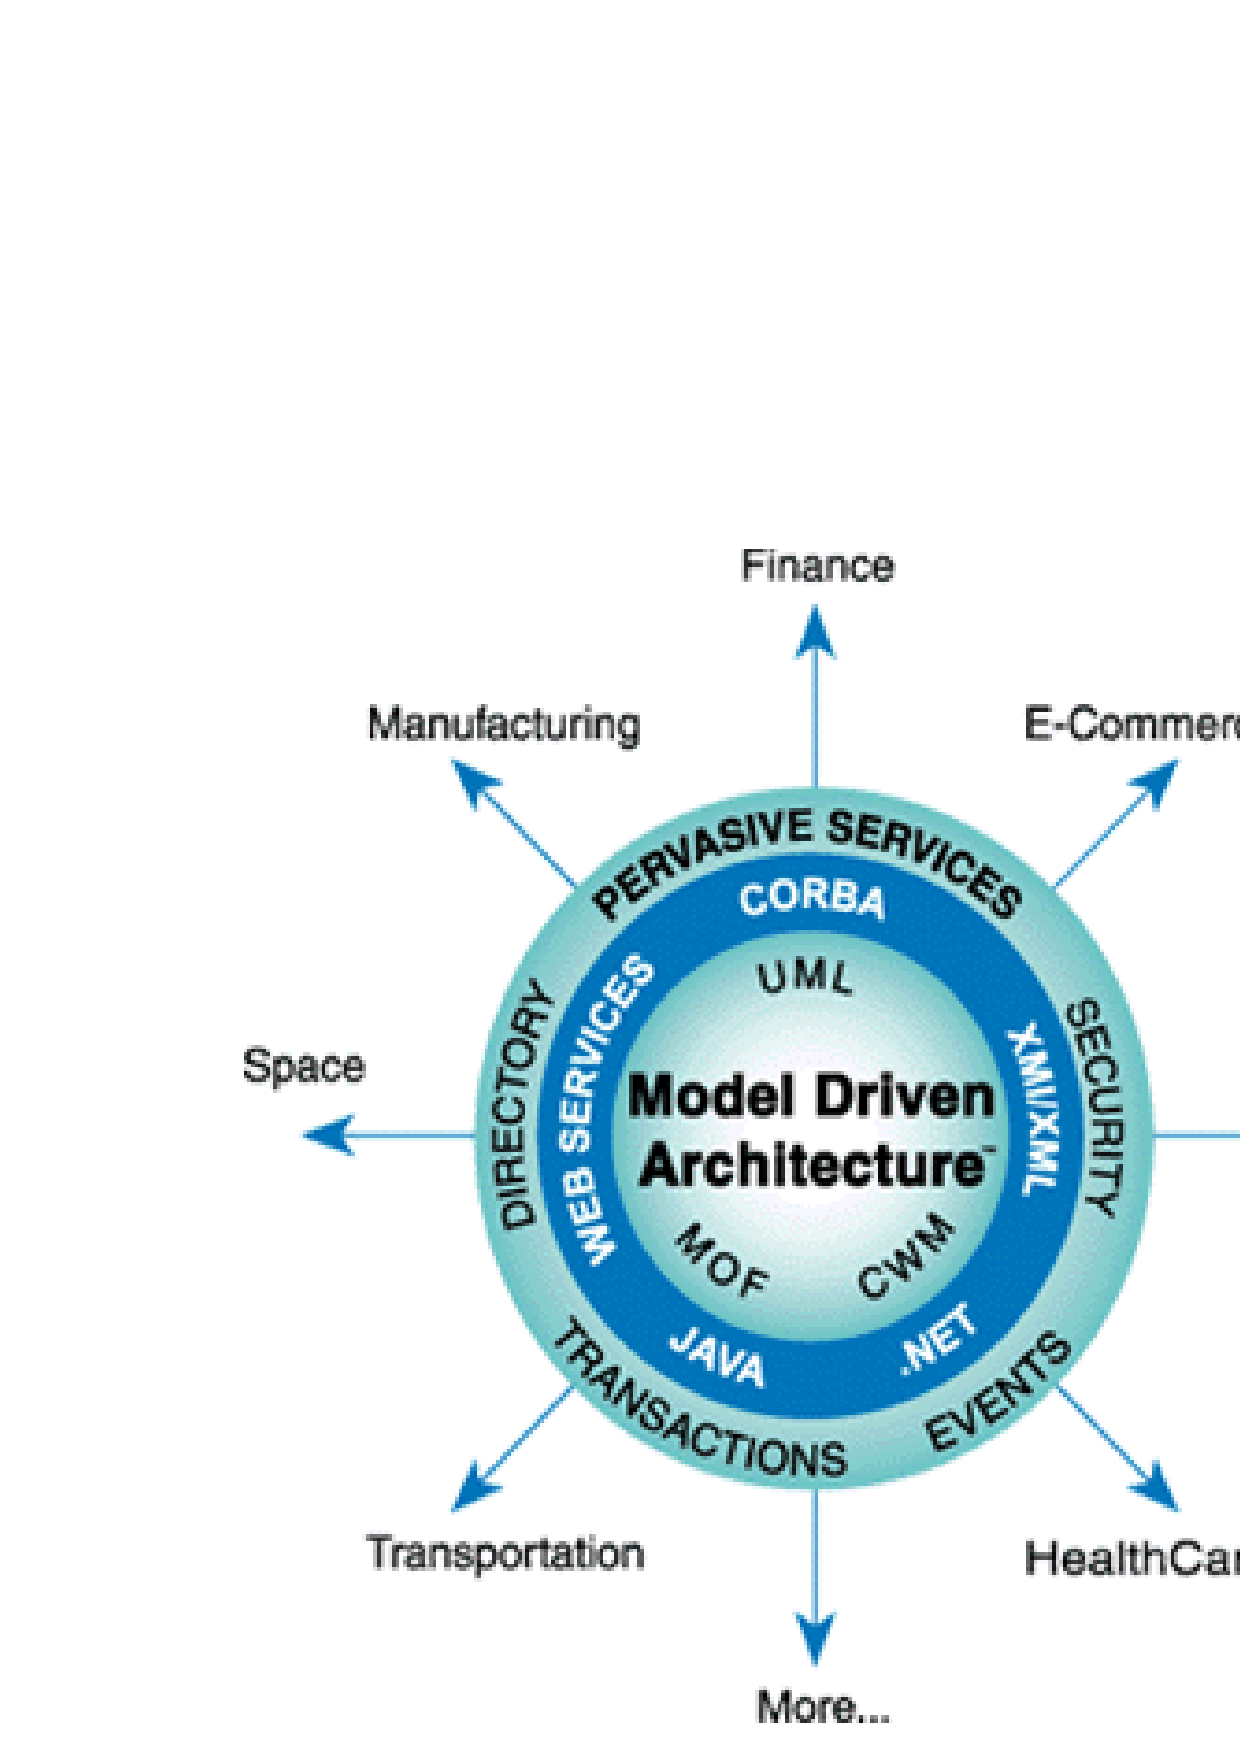
\includegraphics[scale=0.3,angle=-90]{graphic/mda.pdf}
        \caption{Model Driven Architecture \cite{mda}}
        \label{mda_figure}
    \end{center}
\end{figure}

Brown \cite{brown2004} writes: \textit{MDA encourages efficient use of system
models in the software development process, and it supports reuse of best
practices when creating families of systems.} In the OMG's own words, MDA is a:
\textit{way to organise and manage enterprise architectures supported by
automated tools and services for both defining the models and facilitating
transformations between different model types.} It aims at providing an:
\textit{open, vendor-neutral approach to the challenge of business- and
technology change}.

While traditional approaches like \emph{System Family} or
\emph{Tools \& Materials} (section \ref{tool_and_material_heading}) merely
distinguish between \emph{Domain} and \emph{Application}, the conceptual
framework provided by the MDA takes another step in separating abstract
knowledge: It treats \emph{Platform Independent Models} (PIM), that is
business- or application logic, different than the underlying
\emph{Platform Specific Models} (PSM), that is implementation technology. The
translation between the two kinds of models is normally performed using
automated tools for code generation (section \ref{generative_programming_heading}).

The MDA claims to overcome the limitations of implementation
technology-dependent \emph{Computer Aided Software Engineering} (CASE) tools
via standardised mappings and meta architectures \`a la MOF \cite{frankel}.
After Martin Fowler \cite{fowlerdsl}, one argument used in favor of MDA were
that it makes it possible to use \emph{Domain Specific Languages} (DSL)
(section \ref{domain_specific_language_heading}). However, he doubts a success
of the MDA. And indeed, although some MDA standards like the UML are very
sophisticated and widely used, it is still unclear whether the MDA, due to its
complexity, will be able to infiltrate daily software business.

But the idea of separating \emph{Application Knowledge} (PIM) from its
hardware-close \emph{Control and Processing} (PSM) clearly brings a new quality
into software development and is important for later investigations in this
work (chapter \ref{statics_and_dynamics_heading}).

%
% $RCSfile: model_and_code.tex,v $
%
% Copyright (C) 2002-2008. Christian Heller.
%
% Permission is granted to copy, distribute and/or modify this document
% under the terms of the GNU Free Documentation License, Version 1.1 or
% any later version published by the Free Software Foundation; with no
% Invariant Sections, with no Front-Cover Texts and with no Back-Cover
% Texts. A copy of the license is included in the section entitled
% "GNU Free Documentation License".
%
% http://www.cybop.net
% - Cybernetics Oriented Programming -
%
% http://www.resmedicinae.org
% - Information in Medicine -
%
% Version: $Revision: 1.1 $ $Date: 2008-08-19 20:41:07 $ $Author: christian $
% Authors: Christian Heller <christian.heller@tuxtax.de>
%

\subsection{Model and Code}
\label{model_and_code_heading}
\index{Model-Code Synchronisation}
\index{Code Only Approach}
\index{Code Visualisation Approach}
\index{Roundtrip Engineering Approach}
\index{Model Centric Approach}
\index{Model Only Approach}
\index{Model Driven Architecture}
\index{MDA}
\index{Design Phase}
\index{Implementation Phase}
\index{Software Engineering Process}
\index{SEP}

The knowledge abstraction- and implementation techniques considered in the
previous sections belong to the current state-of-the-art in software design and
-modelling, with focus on \emph{Domain Engineering} (DE). Despite some
exceptions like the \emph{Feature Model} (section \ref{feature_model_heading}),
which supports the mapping between abstractions of the analysis- and design
phase, most described techniques deal with bridging the gap between design
models and source code.

\begin{figure}[ht]
    \begin{center}
        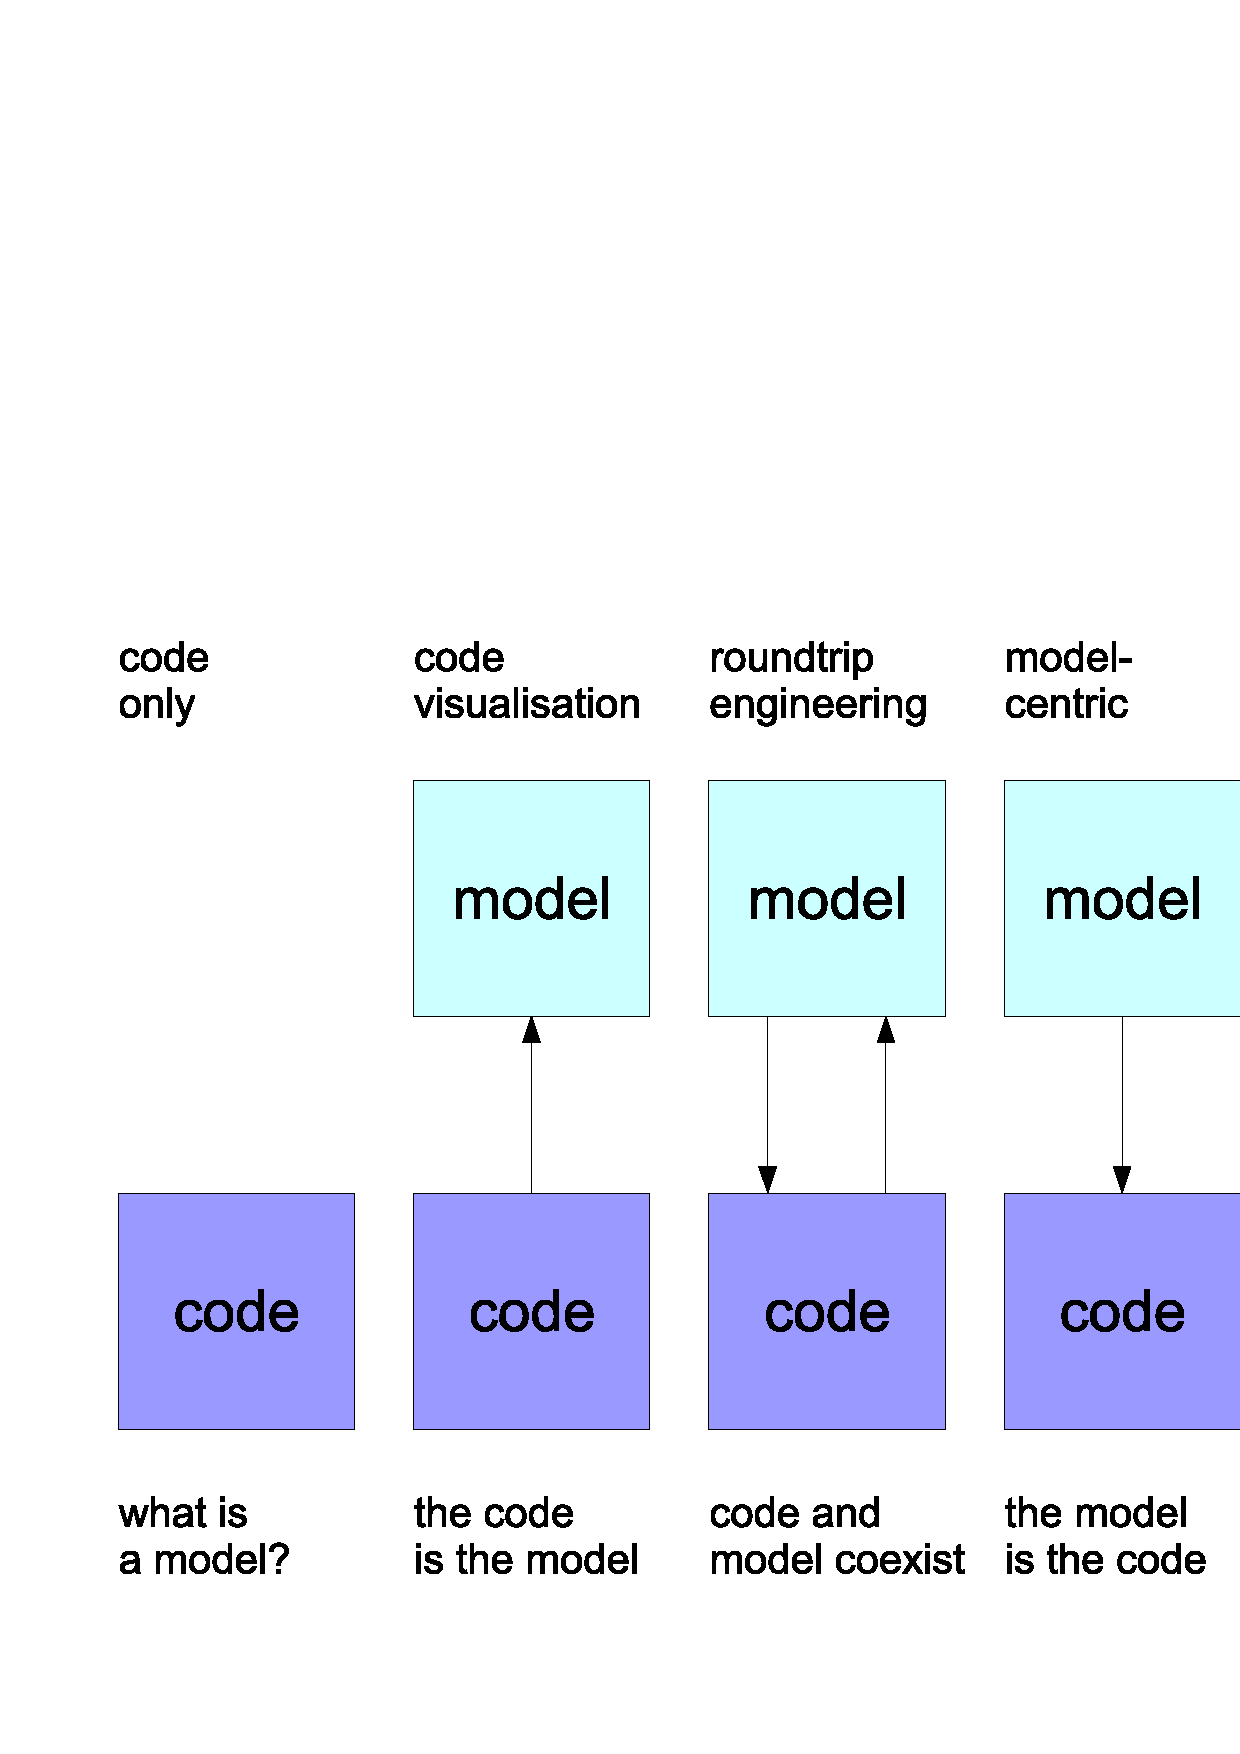
\includegraphics[scale=0.3,angle=-90]{graphic/modelcode.pdf}
        \caption{Model-Code Synchronisation \cite[diagram by John Daniels]{brown2004}}
        \label{modelcode_figure}
    \end{center}
\end{figure}

Alan Brown writes \cite{brown2004}: \textit{One useful way to characterise current
practice is to look at the different ways in which the models are synchronized
with the source code they help describe.} Figure \ref{modelcode_figure} shows
the spectrum of modelling approaches in use today. The different categories
\cite{brown2004} are:

%
% $RCSfile: code_only.tex,v $
%
% Copyright (C) 2002-2008. Christian Heller.
%
% Permission is granted to copy, distribute and/or modify this document
% under the terms of the GNU Free Documentation License, Version 1.1 or
% any later version published by the Free Software Foundation; with no
% Invariant Sections, with no Front-Cover Texts and with no Back-Cover
% Texts. A copy of the license is included in the section entitled
% "GNU Free Documentation License".
%
% http://www.cybop.net
% - Cybernetics Oriented Programming -
%
% http://www.resmedicinae.org
% - Information in Medicine -
%
% Version: $Revision: 1.1 $ $Date: 2008-08-19 20:41:05 $ $Author: christian $
% Authors: Christian Heller <christian.heller@tuxtax.de>
%

\subsubsection{Code Only}
\label{code_only_heading}

\begin{itemize}
    \item[-] almost entire reliance on the code
    \item[-] informal and intuitive modelling of architectural designs
    \item[-] models living on whiteboards, in presentations or the developers' heads
    \item[-] possible use of an \emph{Integrated Development Environment} (IDE)
\end{itemize}

%
% $RCSfile: code_visualisation.tex,v $
%
% Copyright (C) 2002-2008. Christian Heller.
%
% Permission is granted to copy, distribute and/or modify this document
% under the terms of the GNU Free Documentation License, Version 1.1 or
% any later version published by the Free Software Foundation; with no
% Invariant Sections, with no Front-Cover Texts and with no Back-Cover
% Texts. A copy of the license is included in the section entitled
% "GNU Free Documentation License".
%
% http://www.cybop.net
% - Cybernetics Oriented Programming -
%
% http://www.resmedicinae.org
% - Information in Medicine -
%
% Version: $Revision: 1.1 $ $Date: 2008-08-19 20:41:05 $ $Author: christian $
% Authors: Christian Heller <christian.heller@tuxtax.de>
%

\subsubsection{Code Visualisation}
\label{code_visualisation_heading}

\begin{itemize}
    \item[-] alternative modelling using a graphical notation
    \item[-] diagrams aid the understanding of the code's structure or behavior
    \item[-] visual renderings become a direct representation of the code
    \item[-] simultaneous display of code view and model view using
        \emph{Computer Aided Software Engineering} (CASE) tools
\end{itemize}

\input{roundtrip_engineering}
%
% $RCSfile: model_centric.tex,v $
%
% Copyright (C) 2002-2008. Christian Heller.
%
% Permission is granted to copy, distribute and/or modify this document
% under the terms of the GNU Free Documentation License, Version 1.1 or
% any later version published by the Free Software Foundation; with no
% Invariant Sections, with no Front-Cover Texts and with no Back-Cover
% Texts. A copy of the license is included in the section entitled
% "GNU Free Documentation License".
%
% http://www.cybop.net
% - Cybernetics Oriented Programming -
%
% http://www.resmedicinae.org
% - Information in Medicine -
%
% Version: $Revision: 1.1 $ $Date: 2008-08-19 20:41:07 $ $Author: christian $
% Authors: Christian Heller <christian.heller@tuxtax.de>
%

\subsubsection{Model Centric}
\label{model_centric_heading}

\begin{itemize}
    \item[-] sufficiently detailed system models enable the generation of full
        system implementations
    \item[-] models include representations of persistent- and non-persistent
        data, business logic, presentation elements and more
    \item[-] interfaces to legacy systems and various services
    \item[-] specialized tools generate particular (constrained) styles of
        applications, in an automated process
\end{itemize}

\input{model_only}

Considering the developments of the last decades but especially recent years,
the modelling trend clearly goes \emph{left-to-right}, with respect to figure
\ref{modelcode_figure}, that is from \emph{Code only-} to more \emph{Model-centric}
approaches. The emerge of the \emph{Model Driven Architecture} (MDA) (section
\ref{model_driven_architecture_heading}) is one sign therefore. Yet although
these efforts certainly contribute to easier and faster development, less
inter-dependencies within systems, better documentation and clearity of source
code, improved maintenance and more -- the gap between \emph{Design-} and
\emph{Implementation} phase, within a \emph{Software Engineering Process} (SEP)
(chapter \ref{software_engineering_process_heading}), remains. By introducing a
new knowledge schema (chapter \ref{knowledge_schema_heading}), this work wants
to conclusively close gap number \emph{2} (with respect to figure
\ref{gaps_figure} of section \ref{abstraction_gaps_heading}) and provide a
model-only approach.


%
% $RCSfile: knowledge_engineering.tex,v $
%
% Copyright (C) 2002-2008. Christian Heller.
%
% Permission is granted to copy, distribute and/or modify this document
% under the terms of the GNU Free Documentation License, Version 1.1 or
% any later version published by the Free Software Foundation; with no
% Invariant Sections, with no Front-Cover Texts and with no Back-Cover
% Texts. A copy of the license is included in the section entitled
% "GNU Free Documentation License".
%
% http://www.cybop.net
% - Cybernetics Oriented Programming -
%
% http://www.resmedicinae.org
% - Information in Medicine -
%
% Version: $Revision: 1.1 $ $Date: 2008-08-19 20:41:07 $ $Author: christian $
% Authors: Christian Heller <christian.heller@tuxtax.de>
%

\section{Knowledge Engineering}
\label{knowledge_engineering_heading}
\index{Knowledge Engineering}
\index{KE}
\index{Data (Definition)}
\index{Information (Definition)}
\index{Knowledge (Definition)}
\index{Explicit Knowledge}
\index{Implicit Knowledge}
\index{Knowledge Representation}
\index{Date and Rule}

In order to correctly perform information input, memorising, processing and
output, systems need to know about the structure of the data they are
processing. While pure \emph{Data} abstract the real world in form of (mostly
machine-readable) characters (quality) and numbers (quantity) (more on this in
chapter \ref{knowledge_schema_heading}), their interpretation in a semantic
context may yield \emph{Information}. What coincides across the many different
definitions \cite{wikipedia} of the term \emph{Information}, are two
statements: it has to be recognisable and: it has to contain something new.
Organised information available in form of specific structures with
inter-relations is often called \emph{Knowledge}.

Quite often, knowledge gets shared into two kinds: \emph{explicit} (codified)
and \emph{implicit} (tacit). While the former, after \cite{nonaka}, referred to
knowledge that is transmittable in formal, systematic language, the latter had
a personal quality, which made it hard to formalise and communicate. This work
is about explicit knowledge; it wants to provide concepts and schemata for
expressing it as completely as possible (part \ref{contribution_heading}).

Over the years, many different \emph{Knowledge Representation} models have been
proposed. In software engineering, they represent different kinds of user
interfaces (textual, graphical, web), workflows, persistent- or transient data.
The biggest importance, however, models experience when representing a complete
\emph{Domain} (section \ref{domain_model_heading}), that is the special
business field an application system was developed for. After John F. Sowa
\cite{sowa}, \emph{Knowledge Engineering} (KE) could be defined as: \textit{the
branch of engineering that analyses knowledge about some subject and transforms
it to a computable form for some purpose.}

It has to be mentioned that the borders between \emph{Domain Engineering} (DE)
(section \ref{domain_engineering_heading}) and \emph{Knowledge Engineering} are
quite blurry. The \emph{Feature Model} (section \ref{feature_model_heading}),
although described as part of DE, can of course also be seen as one form of
knowledge representation, just like many other models. Both, DE as well as KE
specify formal languages and investigate how different models can be translated
into each other. This work, however, makes a split between DE and KE, because:

\begin{itemize}
    \item[-] their topics are usually treated as different fields of science
    \item[-] KE's focus is almost exclusively on representing (domain)
        knowledge in models
    \item[-] DE also considers their relation to the applications working on
        them
    \item[-] DE distinguishes models belonging to different phases in a
        \emph{Software Engineering Process} (SEP)
    \item[-] DE describes concrete implementation techniques
\end{itemize}

The following sections try to give a brief overview of the rather wide field of
knowledge representation and -engineering, raising only a few topics. Their
main intention is to show the existence of two different kinds of knowledge:
\emph{Date and Rule}, both of which can be structured according to an ontology,
what will be dealt with in the later chapters \ref{knowledge_schema_heading}
and \ref{state_and_logic_heading}.

%\input{undeterministic_knowledge}
%
% $RCSfile: representation_principles.tex,v $
%
% Copyright (C) 2002-2008. Christian Heller.
%
% Permission is granted to copy, distribute and/or modify this document
% under the terms of the GNU Free Documentation License, Version 1.1 or
% any later version published by the Free Software Foundation; with no
% Invariant Sections, with no Front-Cover Texts and with no Back-Cover
% Texts. A copy of the license is included in the section entitled
% "GNU Free Documentation License".
%
% http://www.cybop.net
% - Cybernetics Oriented Programming -
%
% http://www.resmedicinae.org
% - Information in Medicine -
%
% Version: $Revision: 1.1 $ $Date: 2008-08-19 20:41:08 $ $Author: christian $
% Authors: Christian Heller <christian.heller@tuxtax.de>
%

\subsection{Representation Principles}
\label{representation_principles_heading}
\index{Knowledge Representation Principles}
\index{Knowledge Engineering, Basic Principles}

Randall Davis, Howard Schrobe and Peter Szolovits (1993), cited by Sowa in
\cite[p. 134]{sowa}, summarise their review of the state-of-the-art in
knowledge engineering in form of five \emph{Basic Principles}. To them, a
knowledge representation is a:

\begin{enumerate}
    \item \emph{Surrogate:} symbols and the links between them, which form a
        model that simulates a system, serve as surrogates of physical items
        $\rightarrow$ chapter \ref{statics_and_dynamics_heading} will distinguish
        between virtual models (symbols) and real world (physical) items
    \item \emph{Set of ontological commitments:} an ontology determines the
        categories of things that may exist in an application domain
        $\rightarrow$ chapter \ref{knowledge_schema_heading} will introduce a
        knowledge schema permitting to apply an ontological structure to data
    \item \emph{Fragmentary theory of intelligent reasoning:} a description of
        the behaviour and interactions of things in a domain supports reasoning
        about them
        $\rightarrow$ chapter \ref{state_and_logic_heading} will separate state-
        and logic (behavioural) knowledge
    \item \emph{Medium of human expression:} a language facilitates
        communication between knowledge engineers and domain experts
        $\rightarrow$ chapter \ref{cybernetics_oriented_language_heading} will
        define a language for knowledge specification
    \item \emph{Medium for efficient computation:} encoded knowledge ensures
        efficient processing on computing equipment
        $\rightarrow$ chapter \ref{cybernetics_oriented_interpreter_heading} will
        describe a low-level interpreter that processes high-level knowledge
\end{enumerate}

%
% $RCSfile: date_and_rule.tex,v $
%
% Copyright (C) 2002-2008. Christian Heller.
%
% Permission is granted to copy, distribute and/or modify this document
% under the terms of the GNU Free Documentation License, Version 1.1 or
% any later version published by the Free Software Foundation; with no
% Invariant Sections, with no Front-Cover Texts and with no Back-Cover
% Texts. A copy of the license is included in the section entitled
% "GNU Free Documentation License".
%
% http://www.cybop.net
% - Cybernetics Oriented Programming -
%
% http://www.resmedicinae.org
% - Information in Medicine -
%
% Version: $Revision: 1.1 $ $Date: 2008-08-19 20:41:06 $ $Author: christian $
% Authors: Christian Heller <christian.heller@tuxtax.de>
%

\subsection{Date and Rule}
\label{date_and_rule_heading}
\index{Date and Rule}
\index{Expert System}
\index{Relational Database}
\index{Structured Query Language}
\index{SQL}
\index{Existential Conjunctive Logic}
\index{EC Logic}
\index{Modus Ponens, Inference Rule}
\index{Modus Tollens, Inference Rule}
\index{Forward Chaining}
\index{Backward Chaining}
\index{View, Implication}
\index{Trigger, Implication}
\index{Prolog}
\index{Microplanner}
\index{Backtracking}

Two kinds of systems that gained greater popularity are \emph{Expert Systems}
and \emph{Relational Databases}. After Sowa \cite{sowa}, both differed more in
quantity than in quality: \textit{Expert systems use repeated executions of
rules on relatively small amounts of data, while database systems execute short
chains of rules on large amounts of data.} Over time, their differences
decreased and today, the \emph{Structured Query Language} (SQL) for relational
databases supports the same logical functions as early expert systems.

Both, expert systems and relational databases, have common logical foundations
and store data in a subset of logic called \emph{Existential Conjunctive} (EC)
logic. EC is based on two logical operators: the \emph{Existential Quantifier}
$\exists$ and the \emph{Conjunction} $\wedge$; the \emph{Universal Quantifier}
$\forall$ and other operators ($\sim$, $\supset$, $\vee$) are never used.
Sowa \cite[p. 163]{sowa} writes: \textit{While variables in a query are governed
by existential quantifiers, those in a rule are governed by universal quantifiers.}

The two primary inference rules of the above-mentioned systems are called
\emph{Modus Ponens} (putting) and \emph{Modus Tollens} (taking away). Although
being simple, the power of these rules comes from their combination and
repeated execution. While repeated execution of modus ponens is called
\emph{Forward Chaining}, that of modus tollens is called \emph{Backward Chaining}.
In SQL, an implication used in backward chaining is called \emph{View}, and that
used in forward chaining is called \emph{Trigger} \cite{sowa}.

Besides \emph{Prolog} (section \ref{logical_programming_heading}) and \emph{SQL}
(section \ref{data_manipulation_language_heading}), the \emph{Microplanner}
language \cite[p. 157]{sowa} uses the so-called \emph{Backtracking} technique
to answer a query: If one of a sequence of aims cannot be satisfied, the language
tracks back to a previous aim and tries a different option. Although equivalent
queries in Prolog and SQL differ in their syntax, the semantics is the same.
\textit{Logic determines the structure of a query}, as Sowa \cite[p. 159]{sowa}
means.

To sum up, one can say that previous sections distinguished between \emph{Domain-}
and \emph{Application Models}. What was shown in this section, however, is that
many systems and their corresponding languages rely on a separation of \emph{Data}
(in state variables) and \emph{Rules} (logic). This will be of importance in
chapter \ref{state_and_logic_heading}.

%%
% $RCSfile: data_model.tex,v $
%
% Copyright (C) 2002-2008. Christian Heller.
%
% Permission is granted to copy, distribute and/or modify this document
% under the terms of the GNU Free Documentation License, Version 1.1 or
% any later version published by the Free Software Foundation; with no
% Invariant Sections, with no Front-Cover Texts and with no Back-Cover
% Texts. A copy of the license is included in the section entitled
% "GNU Free Documentation License".
%
% http://www.cybop.net
% - Cybernetics Oriented Programming -
%
% http://www.resmedicinae.org
% - Information in Medicine -
%
% Version: $Revision: 1.1 $ $Date: 2008-08-19 20:41:06 $ $Author: christian $
% Authors: Christian Heller <christian.heller@tuxtax.de>
%

\subsection{Data Model}
\label{data_model_heading}

A number of historical and more current domain modelling concepts are described
in brief in the following sections, some of them known from the field of database
technology.

- kind of relationships between the data and rules (knowledge)

%
% $RCSfile: hierarchical_data_model.tex,v $
%
% Copyright (C) 2002-2008. Christian Heller.
%
% Permission is granted to copy, distribute and/or modify this document
% under the terms of the GNU Free Documentation License, Version 1.1 or
% any later version published by the Free Software Foundation; with no
% Invariant Sections, with no Front-Cover Texts and with no Back-Cover
% Texts. A copy of the license is included in the section entitled
% "GNU Free Documentation License".
%
% http://www.cybop.net
% - Cybernetics Oriented Programming -
%
% http://www.resmedicinae.org
% - Information in Medicine -
%
% Version: $Revision: 1.1 $ $Date: 2008-08-19 20:41:07 $ $Author: christian $
% Authors: Christian Heller <christian.heller@tuxtax.de>
%

\subsubsection{Hierarchical Data Model}
\label{hierarchical_data_model_heading}

One of the first models to structure domain data was a simple \emph{Hierarchy},
being used in \emph{Hierarchical Databases} such as ... (VSAM),
in the 1960s and early 1970s. Many of them are still running now,
for instance in insurance companies who have not yet migrated their
systems to modern technologies.

Knowledge Engineering Systems make use of hierarchical data, today.

- Domain Engineering in general, vertical and horizontal separation
- see \cite{inpulse} paper

The following techniques of domain modelling are neither sorted historically,
nor after the SEP phase they are used in (analysis, design, implementation).
The order of their appearance is determined by similarities they have. New
techniques are added stepwise, in a didactic manner, one building on the
other.

The feature modelling, for example, is a domain analysis- and not an
implementation technique but mentioned here because it is based on a special
technique of abstraction worth considering. Moreover it is not exclusively used
for analysis, but also it represents the beginning of design in a software
engineering process, as mentioned in section \ref{abstraction_gaps_heading}.

- add Feature Model to domain modelling, because it is a hierarchical model

\input{network_data_model}
\input{entity_relationship_model}
%
% $RCSfile: object_oriented_model.tex,v $
%
% Copyright (C) 2002-2008. Christian Heller.
%
% Permission is granted to copy, distribute and/or modify this document
% under the terms of the GNU Free Documentation License, Version 1.1 or
% any later version published by the Free Software Foundation; with no
% Invariant Sections, with no Front-Cover Texts and with no Back-Cover
% Texts. A copy of the license is included in the section entitled
% "GNU Free Documentation License".
%
% http://www.cybop.net
% - Cybernetics Oriented Programming -
%
% http://www.resmedicinae.org
% - Information in Medicine -
%
% Version: $Revision: 1.1 $ $Date: 2008-08-19 20:41:07 $ $Author: christian $
% Authors: Christian Heller <christian.heller@tuxtax.de>
%

\subsubsection{Object Oriented Model}
\label{object_oriented_model_heading}

?? frame \cite{sowa}, as ancestor of OO and others

The introduction of object oriented programming (section
\ref{object_oriented_programming_heading}) made another software design
philosophy popular:
Every entity was now treated as \emph{Object} being a runtime-instance of a
\emph{Class} that was capable of inheriting \emph{Attributes} and \emph{Methods}
from a parent class. A \emph{Relation} was now called \emph{Association}.
Multiplicity was called \emph{Cardinality}.

The primary new ideas of \emph{Inheritance} between classes and classes owning not
only attributes but also \emph{Methods} could not be modeled well in entity relationship
models (section \ref{entity_relationship_model}) so that \emph{Data Mapper} layers
(section \ref{data_mapper_heading}) became necessary. In general, object oriented
models look not much different from entity relationship models.


%%
% $RCSfile: knowledge_map.tex,v $
%
% Copyright (C) 2002-2008. Christian Heller.
%
% Permission is granted to copy, distribute and/or modify this document
% under the terms of the GNU Free Documentation License, Version 1.1 or
% any later version published by the Free Software Foundation; with no
% Invariant Sections, with no Front-Cover Texts and with no Back-Cover
% Texts. A copy of the license is included in the section entitled
% "GNU Free Documentation License".
%
% http://www.cybop.net
% - Cybernetics Oriented Programming -
%
% http://www.resmedicinae.org
% - Information in Medicine -
%
% Version: $Revision: 1.1 $ $Date: 2008-08-19 20:41:07 $ $Author: christian $
% Authors: Christian Heller <christian.heller@tuxtax.de>
%

\subsection{Knowledge Map}
\label{knowledge_map_heading}

A \emph{Topic Map} is ... a standard paradigm for the interchange of knowledge structures.
http://www.topicmaps.org/
http://topicmap.com/topicmap/tools.html

A \emph{Concept Map} is a diagram meant to represent ideas, each idea being
represented by a shape (rectangle, ellipse, image, ...). The diagram becomes
a concept map when relations link these ideas and \emph{Hypertext Links} are
added to these ideas which allows navigation to either a detailed description,
for example a web page providing details on this idea, or another concept map.
\cite{} [http://www.thinkgraph.com/english/index.htm]

A \emph{Mind Map} is a powerful graphic technique which provides a universal
key to unlock the potential of the brain. It harnesses the full range of cortical
skills -- word, image, number, logic, rhythm, colour and spatial awareness --
in a single, uniquely powerful manner. In so doing, it gives you the freedom
to roam the infinite expanses of your brain. The Mind Map can be applied to
every aspect of life where improved learning and clearer thinking will enhance
human performance.
\cite{} [http://www.mind-map.com/EN/mindmaps/definition.html]

A \emph{Mind Map} is a picture that represents semantic connections between
portions of learned material.
\cite[http://en.wikipedia.org/wiki/Mind_mapping]{wikipedia}

https://sourceforge.net/projects/freemind/

%
% $RCSfile: agent_communication_language.tex,v $
%
% Copyright (C) 2002-2008. Christian Heller.
%
% Permission is granted to copy, distribute and/or modify this document
% under the terms of the GNU Free Documentation License, Version 1.1 or
% any later version published by the Free Software Foundation; with no
% Invariant Sections, with no Front-Cover Texts and with no Back-Cover
% Texts. A copy of the license is included in the section entitled
% "GNU Free Documentation License".
%
% http://www.cybop.net
% - Cybernetics Oriented Programming -
%
% http://www.resmedicinae.org
% - Information in Medicine -
%
% Version: $Revision: 1.1 $ $Date: 2008-08-19 20:41:05 $ $Author: christian $
% Authors: Christian Heller <christian.heller@tuxtax.de>
%

\subsection{Agent Communication Language}
\label{agent_communication_language_heading}
\index{Agent Communication Language}
\index{ACL}
\index{Artificial Intelligence}
\index{AI}
\index{Agent Oriented Programming}
\index{AGOP}

A whole palette of languages was suggested within the scientific field of
\emph{Artificial Intelligence} (AI). \emph{Agent Oriented Programming} (AGOP)
(section \ref{agent_oriented_programming_heading}), for example, uses
representation formats like the ones described following, for the knowledge
bases and communication of its agent systems. That is why such formats are
often labeled \emph{Agent Communication Language} (ACL).

%
% $RCSfile: knowledge_interchange_format.tex,v $
%
% Copyright (C) 2002-2008. Christian Heller.
%
% Permission is granted to copy, distribute and/or modify this document
% under the terms of the GNU Free Documentation License, Version 1.1 or
% any later version published by the Free Software Foundation; with no
% Invariant Sections, with no Front-Cover Texts and with no Back-Cover
% Texts. A copy of the license is included in the section entitled
% "GNU Free Documentation License".
%
% http://www.cybop.net
% - Cybernetics Oriented Programming -
%
% http://www.resmedicinae.org
% - Information in Medicine -
%
% Version: $Revision: 1.1 $ $Date: 2008-08-19 20:41:07 $ $Author: christian $
% Authors: Christian Heller <christian.heller@tuxtax.de>
%

\subsubsection{Knowledge Interchange Format}
\label{knowledge_interchange_format_heading}
\index{Knowledge Interchange Format}
\index{KIF}
\index{PostScript}
\index{PS}

The \emph{Knowledge Interchange Format} (KIF), as described in \cite{kif}, is:

\begin{itemize}
    \item[-] a language designed for use in the interchange of knowledge among
        disparate computer systems
    \item[-] not intended as a primary language for interaction with human users
    \item[-] not intended as an internal representation for knowledge within
        computer systems
    \item[-] in its purpose, roughly analogous to \emph{PostScript} (PS)
        (section \ref{page_description_language_heading})
    \item[-] not as efficient as a specialised representation for knowledge,
        but more general and programmer-readable
\end{itemize}

The idea behind KIF is that \cite{kif}: \textit{a computer system reads a
knowledge base in KIF, (and) converts the data into its own internal form
(pointer structures, arrays, etc.). All computation is done using these
internal forms. When the computer system needs to communicate with another
computer system, it maps its internal data structures into KIF.} KIF's design
is characterised by three features:

\begin{enumerate}
    \item \emph{Declarative Semantics:} independent from specific interpreters,
        as opposed to e.g. \emph{Prolog}
    \item \emph{Logically Comprehensive:} may express arbitrary logical
        sentences, as opposed to \emph{SQL} or \emph{Prolog}
    \item \emph{Meta Knowledge:} permits the introduction of new knowledge
        representation constructs, without changing the language
\end{enumerate}

The following syntax example \cite{kif} shows a logical term involving the
\emph{if} operator. If the object constant \emph{a} denotes a number, then the
term denotes the absolute value of that number:

\begin{scriptsize}
    \begin{verbatim}
    (if (> a 0) a (- a))
    \end{verbatim}
\end{scriptsize}

The language introduced in chapter \ref{cybernetics_oriented_language_heading}
may not only serve as interchange format between systems, but also for the
definition of user interfaces, workflows and domain models, altogether. It
treats state- and logic models as separate, composable concepts (chapter
\ref{state_and_logic_heading}), which KIF does not. Further, it provides the
means to express meta knowledge.

%
% $RCSfile: knowledge_query_and_manipulation_language.tex,v $
%
% Copyright (C) 2002-2008. Christian Heller.
%
% Permission is granted to copy, distribute and/or modify this document
% under the terms of the GNU Free Documentation License, Version 1.1 or
% any later version published by the Free Software Foundation; with no
% Invariant Sections, with no Front-Cover Texts and with no Back-Cover
% Texts. A copy of the license is included in the section entitled
% "GNU Free Documentation License".
%
% http://www.cybop.net
% - Cybernetics Oriented Programming -
%
% http://www.resmedicinae.org
% - Information in Medicine -
%
% Version: $Revision: 1.1 $ $Date: 2008-08-19 20:41:07 $ $Author: christian $
% Authors: Christian Heller <christian.heller@tuxtax.de>
%

\subsubsection{Knowledge Query and Manipulation Language}
\label{knowledge_query_and_manipulation_language_heading}
\index{Knowledge Query and Manipulation Language}
\index{KQML}
\index{Common Lisp}
\index{CL}

The \emph{Knowledge Query and Manipulation Language} (KQML) \cite{kqml} is a:
\textit{language and associated protocol by which intelligent software agents
can communicate to share information and knowledge}, as Tim Finin et al.
\cite{finin} write. Its syntax were based on a balanced parenthesis list,
because initial implementations had been done in Common Lisp (CL)
\cite{commonlisp}. After Finin et al., the initial element of the list were the
\emph{Performative} and the remaining elements were the performative's
\emph{Arguments} as keyword/ value pairs. The Free Wikipedia Encyclopedia
\cite{wikipedia} explains:

\begin{quote}
    The KQML message format and protocol can be used to interact with an
    intelligent system, either by an application program, or by another
    intelligent system. KQML's \emph{Performatives} are operations that agents
    perform on each other's \emph{Knowledge} and \emph{Goal} stores.
    Higher-level interactions such as \emph{Contract Nets} and
    \emph{Negotiation} are built using these. KQML's
    \emph{Communication Facilitators} coordinate the interactions of other
    agents to support \emph{Knowledge Sharing}.
\end{quote}

An example message representing a query about the price of a share of IBM stock
might be encoded as \cite{finin}:

\begin{scriptsize}
    \begin{verbatim}
    (ask-one
    :content (PRICE IBM ?price)
    :receiver stock-server
    :language LPROLOG
    :ontology NYSE-TICKS)
    \end{verbatim}
\end{scriptsize}

System communication and its elements like \emph{Sender}, \emph{Receiver},
\emph{Language} or \emph{Message Content} will be further investigated in
chapter \ref{state_and_logic_heading}. The new language introduced in chapter
\ref{cybernetics_oriented_language_heading} defines communication operations
(logic) accompanied by properties (meta information), much the same way
performatives have arguments. Also, that new language may not only be used to
encode knowledge for communication, but to represent knowledge of arbitrary
domains. By combining pre-defined, primitive operations, it may be used to
create more complex (higher-level) algorithms.

%
% $RCSfile: darpa_agent_markup_language.tex,v $
%
% Copyright (C) 2002-2008. Christian Heller.
%
% Permission is granted to copy, distribute and/or modify this document
% under the terms of the GNU Free Documentation License, Version 1.1 or
% any later version published by the Free Software Foundation; with no
% Invariant Sections, with no Front-Cover Texts and with no Back-Cover
% Texts. A copy of the license is included in the section entitled
% "GNU Free Documentation License".
%
% http://www.cybop.net
% - Cybernetics Oriented Programming -
%
% http://www.resmedicinae.org
% - Information in Medicine -
%
% Version: $Revision: 1.1 $ $Date: 2008-08-19 20:41:06 $ $Author: christian $
% Authors: Christian Heller <christian.heller@tuxtax.de>
%

\subsubsection{DARPA Agent Markup Language / Ontology Inference Layer}
\label{darpa_agent_markup_language_heading}
\index{DARPA Agent Markup Language}
\index{DAML}
\index{Ontology Inference Layer}
\index{OIL}
\index{DAML+OIL}
\index{Semantic Web}
\index{Extensible Markup Language}
\index{XML}
\index{Resource Description Framework}
\index{RDF}
\index{OWL}

The DAML+OIL language resulted from a combination of the DAML and OIL languages.
The \emph{DARPA Agent Markup Language} (DAML) \cite{damloil} was created in a
project run by the \emph{Defense Advanced Research Projects Agency} (DARPA) of the
\emph{United States of America} (USA); the \emph{Ontology Inference Layer} (OIL)
was created within the \emph{Information Science Technologies} (IST) program of
the \emph{European Union} (EU) \cite{rdfowlrelease}. Both projects aimed at
developing a language and tools to facilitate the concept of the
\emph{Semantic Web} (section \ref{semantic_web_heading}).

At the beginning of the project stood the realisation that: \textit{The use of
ontologies (section \ref{conceptual_network_heading}) provides a very powerful
way to describe objects and their relationships to other objects.} The DAML+OIL
language, being developed as an extension to the \emph{Extensible Markup Language}
(XML) (section \ref{extensible_markup_language_heading}) and the
\emph{Resource Description Framework} (RDF) (section \ref{semantic_web_heading}),
therefore provided a \cite{rdf} rich set of constructs with which to create
ontologies and to markup information so that it becomes machine-readable and
understandable. Much of the work in DAML and OIL has now been incorporated into
OWL (section \ref{web_ontology_language_heading}).

Chapter \ref{cybernetics_oriented_language_heading} will introduce a language
that is based on XML, too.

%\input{general_ontological_language}
%\emph{General Ontological Language} (GOL) \cite{degen}
%Dokument dazu liegt lokal in /tmp:
%explanation of KIF etc.; Sowa is referenced; see end of paper for relation to informatics

%
% $RCSfile: semantic_web.tex,v $
%
% Copyright (C) 2002-2008. Christian Heller.
%
% Permission is granted to copy, distribute and/or modify this document
% under the terms of the GNU Free Documentation License, Version 1.1 or
% any later version published by the Free Software Foundation; with no
% Invariant Sections, with no Front-Cover Texts and with no Back-Cover
% Texts. A copy of the license is included in the section entitled
% "GNU Free Documentation License".
%
% http://www.cybop.net
% - Cybernetics Oriented Programming -
%
% http://www.resmedicinae.org
% - Information in Medicine -
%
% Version: $Revision: 1.1 $ $Date: 2008-08-19 20:41:08 $ $Author: christian $
% Authors: Christian Heller <christian.heller@tuxtax.de>
%

\subsection{Semantic Web}
\label{semantic_web_heading}
\index{Semantic Web}
\index{Extensible Markup Language}
\index{XML}
\index{XML Schema}
\index{XML Data}
\index{Document Content Description}
\index{DCD}
\index{Schema for Object Oriented XML}
\index{SOX}
\index{XML Metadata Interchange}
\index{XMI}
\index{Resource Description Framework}
\index{RDF}
\index{Web Ontology Language}
\index{OWL}

As mentioned in section \ref{extensible_markup_language_heading}, the
\emph{Extensible Markup Language} (XML) \cite{rdfowlrelease} provides a:
\textit{set of rules for creating vocabularies that can bring structure to both
documents and data on the Web} and it: \textit{gives clear rules for syntax.}
XML Schemas \cite{xmlschema} served as: \textit{a method for composing XML
vocabularies.} Yet although XML were a powerful, flexible surface syntax for
structured documents, it imposed no \emph{Semantic Constraints} on the
\emph{Meaning} of these documents. Having investigated the usefulness of XML
for a \emph{meaningful} sharing of information units at the semantic level,
Robin Cover writes \cite{xmlsemantics}:

\begin{quote}
    \ldots\ the use of XML for \emph{Data Interchange} may already outweigh its
    use for \emph{Document Display}. For messaging and other transaction data,
    specifications approaching the level of formal semantics (e.g. KIF or KQML)
    are desirable, governing not just common (atomic) data types in business
    objects, but complex objects used by computer agents in large-scale business
    transactions. XML vocabularies supporting these applications will need to be
    defined in terms of precise object semantics.
\end{quote}

He lists a number of efforts dealing with the support for generic XML semantics,
that is \emph{Semantic Transparency} of XML in a broader sense, to provide
unambiguous semantic specification:

\begin{itemize}
    \item[-] \emph{XML Data} \cite{xmldata}
    \item[-] \emph{Document Content Description} (DCD) for XML \cite{dcd}
    \item[-] \emph{Schema for Object Oriented XML} (SOX) \cite{sox}
    \item[-] \emph{XML Metadata Interchange} (XMI) \cite{mda}
    \item[-] \emph{Resource Description Framework} (RDF) \cite{rdf}
    \item[-] \emph{Web Ontology Language} (OWL) \cite{owl}
\end{itemize}

The RDF and OWL as well-known efforts are mentioned in the following two
subsections. Both are often comprised under the umbrella term
\emph{Semantic Web}. Much of what is written about the semantic web sounds as
if it was a replacement technology for the Web as known today. Yet Eric Miller,
leader of W3C's semantic web activity, means \cite{rdfowlrelease}:

\begin{quote}
    In reality, it's more Web Evolution than Revolution. The Semantic Web is
    made through incremental changes, by bringing machine-readable descriptions
    to the data and documents already on the Web. XML, RDF and OWL enable the
    Web to be a global infrastructure for sharing both, documents and data which
    make searching and reusing information easier and more reliable as well.
\end{quote}

%
% $RCSfile: resource_description_framework.tex,v $
%
% Copyright (C) 2002-2008. Christian Heller.
%
% Permission is granted to copy, distribute and/or modify this document
% under the terms of the GNU Free Documentation License, Version 1.1 or
% any later version published by the Free Software Foundation; with no
% Invariant Sections, with no Front-Cover Texts and with no Back-Cover
% Texts. A copy of the license is included in the section entitled
% "GNU Free Documentation License".
%
% http://www.cybop.net
% - Cybernetics Oriented Programming -
%
% http://www.resmedicinae.org
% - Information in Medicine -
%
% Version: $Revision: 1.1 $ $Date: 2008-08-19 20:41:08 $ $Author: christian $
% Authors: Christian Heller <christian.heller@tuxtax.de>
%

\subsubsection{Resource Description Framework}
\label{resource_description_framework_heading}
\index{Resource Description Framework}
\index{RDF}
\index{Extensible Markup Language}
\index{XML}
\index{RDF Schema}
\index{XML Schema}
\index{OWL}

The \emph{Resource Description Framework} (RDF) \cite{rdf} as part of the
\emph{Semantic Web} provides a standard way for simple descriptions to be made.
It is: \textit{a simple data model for referring to objects (resources) and how
they are related. An RDF-based model can be represented in XML syntax.}
\cite{wikipedia}

RDF wants to achieve for \emph{Semantics} what XML has achieved for
\emph{Syntax} -- to provide a clear set of rules for creating descriptive
information. Both follow a special schema, \emph{RDF Schema} \cite{rdf} and
\emph{XML Schema} \cite{xmlschema}, respectively, which defines the structure
and vocabulary that may be used in the corresponding documents.

Many applications that use XML as syntax for data interchange, may apply the
RDF specifications to better support the exchange of actual knowledge on the
web. The RDF data framework is used \cite{rdfowlrelease} in: asset management,
enterprise integration and the sharing and reuse of data on the web. Example
applications combining information from multiple sources on the web
\cite{rdfowlrelease} include: library catalogs, world-wide directories, news-
and content aggregation, collections of music or photos.

In the words of Brian McBride \cite{rdfowlrelease}, chair of the RDF core
working group, his group had: \textit{turned the RDF specifications into both a
practical and mathematically precise foundation on which OWL and the rest of
the semantic web can be built.}

Chapter \ref{cybernetics_oriented_language_heading} will come back to RDF once
more, and compare it with the new language then introduced.

%
% $RCSfile: web_ontology_language.tex,v $
%
% Copyright (C) 2002-2008. Christian Heller.
%
% Permission is granted to copy, distribute and/or modify this document
% under the terms of the GNU Free Documentation License, Version 1.1 or
% any later version published by the Free Software Foundation; with no
% Invariant Sections, with no Front-Cover Texts and with no Back-Cover
% Texts. A copy of the license is included in the section entitled
% "GNU Free Documentation License".
%
% http://www.cybop.net
% - Cybernetics Oriented Programming -
%
% http://www.resmedicinae.org
% - Information in Medicine -
%
% Version: $Revision: 1.1 $ $Date: 2008-08-19 20:41:09 $ $Author: christian $
% Authors: Christian Heller <christian.heller@tuxtax.de>
%

\subsubsection{Web Ontology Language}
\label{web_ontology_language_heading}
\index{Web Ontology Language}
\index{OWL}
\index{Uniform Resource Indicator}
\index{URI}
\index{Resource Description Framework}
\index{RDF}
\index{DARPA Agent Markup Language}
\index{Ontology Inference Layer}
\index{DAML+OIL}
\index{Ontology}

The \emph{Web Ontology Language} (OWL) is \cite{owl}: \textit{a semantic markup
language for publishing and sharing ontologies on the world wide web \ldots\
which delivers richer integration and interoperability of data among descriptive
communities.} It uses \emph{Uniform Resource Indicators} (URI) for naming and
is an extension of the \emph{Resource Description Framework} (RDF), adding more
vocabulary for describing properties and classes, for example relations between
classes, cardinality, richer typing of properties, or enumerated classes. OWL
was originally derived from the \emph{DARPA Agent Markup Language} +
\emph{Ontology Inference Layer} (DAML+OIL) web ontology language (section
\ref{agent_communication_language_heading}).

In the understanding of OWL, an ontology is a subject- or domain specific
vocabulary which defines the terms used to describe and represent an area of
knowledge \cite{rdfowlrelease}. However, there are other definitions of the term
\emph{Ontology} which are given in section \ref{conceptual_network_heading}.
OWL aims to add to ontologies capabilities like \cite{rdfowlrelease}:

\begin{itemize}
    \item[-] Ability to be distributed across many systems
    \item[-] Scalability to web needs
    \item[-] Compatibility with web standards for accessibility and internationalisation
    \item[-] Openness and extensibility
\end{itemize}

It introduces keywords for the use of \emph{Classification}, \emph{Subclassing}
with \emph{Inheritance} and further abstraction principles. RDF is neutral
enough to permit such extensions. Also the language introduced in chapter
\ref{cybernetics_oriented_language_heading} may be extended with meta
properties, such as one for inheritance.


%\input{temporary_section_summary}

%
% $RCSfile: conceptual_network.tex,v $
%
% Copyright (C) 2002-2008. Christian Heller.
%
% Permission is granted to copy, distribute and/or modify this document
% under the terms of the GNU Free Documentation License, Version 1.1 or
% any later version published by the Free Software Foundation; with no
% Invariant Sections, with no Front-Cover Texts and with no Back-Cover
% Texts. A copy of the license is included in the section entitled
% "GNU Free Documentation License".
%
% http://www.cybop.net
% - Cybernetics Oriented Programming -
%
% http://www.resmedicinae.org
% - Information in Medicine -
%
% Version: $Revision: 1.1 $ $Date: 2008-08-19 20:41:06 $ $Author: christian $
% Authors: Christian Heller <christian.heller@tuxtax.de>
%

\section{Conceptual Network}
\label{conceptual_network_heading}
\index{Conceptual Network}
\index{Ontology}

John F. Sowa \cite{sowa} cites the computer science pioneer Alan Perlis who,
being asked whether a computer could automatically write programs from informal
specifications, replied: \textit{It is not possible to translate informal
specifications to formal specifications by any formal algorithm.} And Sowa
writes on: \textit{English syntax is not what makes the translation difficult.
The difficulty results from the enormous amount of background knowledge that
lies behind every word.}

The structuring of such knowledge is what \emph{Ontologies} shall support. They
are the topic of the following sections and will be of importance for the
knowledge schema introduced in chapter \ref{knowledge_schema_heading}.

%
% $RCSfile: ontos_and_logos.tex,v $
%
% Copyright (C) 2002-2008. Christian Heller.
%
% Permission is granted to copy, distribute and/or modify this document
% under the terms of the GNU Free Documentation License, Version 1.1 or
% any later version published by the Free Software Foundation; with no
% Invariant Sections, with no Front-Cover Texts and with no Back-Cover
% Texts. A copy of the license is included in the section entitled
% "GNU Free Documentation License".
%
% http://www.cybop.net
% - Cybernetics Oriented Programming -
%
% http://www.resmedicinae.org
% - Information in Medicine -
%
% Version: $Revision: 1.1 $ $Date: 2008-08-19 20:41:08 $ $Author: christian $
% Authors: Christian Heller <christian.heller@tuxtax.de>
%

\subsection{Ontos and Logos}
\label{ontos_and_logos_heading}
\index{Ontos and Logos}
\index{Ontology}
\index{Metaphysics}
\index{Agent Communication Language}
\index{ACL}
\index{Semantic Web}
\index{Terminology}

The word \emph{Ontology} stems from ancient Greek language, consisting of the
two subterms \emph{Ontos} and \emph{Logos} which literally mean \emph{Stone} (in
the meaning of \emph{Being}) and \emph{Word} (in the meaning of \emph{Study}).
Thus, ontology designates \emph{the study of the nature of reality}.

Manifold, more detailed definitions are given in literature. They mostly relate
to one of the subjects, \emph{Philosophy} or \emph{Information Technology}
(IT). A philosophical one that can be found in Smith and Welty \cite{smith}
says: Ontology is \emph{the science of what is, of the kinds and structures of
objects, properties, events, processes and relations in every area of reality}.
Since what it means for something \emph{to be} or \emph{to be real} were an
issue beyond what is physically accessible, as Daniel \cite{daniel} writes,
ontological questions were \emph{metaphysical}. \emph{Metaphysics} included not
only the study of being and reality but also \emph{the study of specific kinds
of beings}, such as minds. Metaphysics in general and ontology in particular
were both interested in providing a \emph{Logos}, a rational explanation for
existence. The Dictionary of Philosophy of Mind \cite{pomdictionary}, as
further source, states:

\begin{quote}
    Although the term terms \emph{Ontology} and \emph{Metaphysics} are far from
    being univocal and determinate in philosophical jargon, an important
    distinction seems often enough to be marked by them. What we may call
    ontology is the attempt to say what entities exist. Metaphysics, by
    contrast, is the attempt to say, of those entities, what they are. In
    effect, one's ontology is one's \emph{List} of entities, while one's
    metaphysics is an explanatory theory about the \emph{Nature} of those
    entities.
\end{quote}

Besides rather philosophical descriptions, Eric Little \cite{little} also
quotes a more information science-like definition of Gruber \cite{gruber} for
whom an ontology is an: \textit{explicit specification of a conceptualization}
(of a domain), in other words a \emph{formalisation of domain knowledge}. For
the \emph{Ontology Forum} \cite{ontologyorg}, the key ingredients that made up
an ontology were a \textit{vocabulary of basic terms} and a \textit{precise
specification of what those terms mean}. The \emph{Agent Communication Languages}
(ACL) and \emph{Semantic Web} technologies, introduced in sections
\ref{agent_communication_language_heading} and \ref{semantic_web_heading},
respectively, use ontologies in the same meaning. The borders to
\emph{Terminology} (section \ref{terminology_heading}) are often blurry.

The knowledge schema and new language of chapters \ref{knowledge_schema_heading}
and \ref{cybernetics_oriented_language_heading} may represent entity
information (an ontology) as well as meta information about these (metaphysical
explanations). However, in order to avoid conflicts with philosophy, this work
sticks to Gruber's definition of the term \emph{Ontology}, for the time being,
until it defines it in its own way, in chapter \ref{knowledge_schema_heading}.

%
% $RCSfile: applicability.tex,v $
%
% Copyright (C) 2002-2008. Christian Heller.
%
% Permission is granted to copy, distribute and/or modify this document
% under the terms of the GNU Free Documentation License, Version 1.1 or
% any later version published by the Free Software Foundation; with no
% Invariant Sections, with no Front-Cover Texts and with no Back-Cover
% Texts. A copy of the license is included in the section entitled
% "GNU Free Documentation License".
%
% http://www.cybop.net
% - Cybernetics Oriented Programming -
%
% http://www.resmedicinae.org
% - Information in Medicine -
%
% Version: $Revision: 1.1 $ $Date: 2008-08-19 20:41:05 $ $Author: christian $
% Authors: Christian Heller <christian.heller@tuxtax.de>
%

\subsection{Applicability}
\label{applicability_heading}
\index{Artificial Intelligence}
\index{AI}

The \emph{Ontology Forum} \cite{ontologyorg} writes that ontologies find
applicability in many areas of information systems engineering, for example in
database design, in object systems, in knowledge based systems and within many
application areas such as datawarehousing, knowledge management, computer
supported collaborative working and enterprise integration. Depending on the
nature of the knowledge they were concerned with, communities would differ:

\begin{itemize}
    \item[-] \emph{Artificial Intelligence} (AI): ontologies capture domain
        knowledge, while problem-solving methods capture task knowledge
    \item[-] \emph{Natural Language}: ontologies characterise word meaning and
        sense
    \item[-] \emph{Database}: ontologies, as conceptual schema, provide semantic
        inter-operability of heterogeneous databases
    \item[-] \emph{Object Oriented Design Methods}: ontologies, as domain models,
        specify software systems that need not be knowledge-based
\end{itemize}

Sections \ref{agent_communication_language_heading} and \ref{semantic_web_heading}
mentioned the use of ontologies for semantic-based information retrieval. What
(conceptually) unites these communities, is the ability of ontologies to reduce
semantic ambiguity for the purpose of sharing and reusing knowledge, to achieve
inter-operability. In the context of this work, ontologies are mainly used to
structure domain knowledge meaningfully, in levels of growing granularity, with
unidirectional relations from higher-level layers to layers of lower
granularity (chapter \ref{knowledge_schema_heading}).

%
% $RCSfile: two_level_separation.tex,v $
%
% Copyright (C) 2002-2008. Christian Heller.
%
% Permission is granted to copy, distribute and/or modify this document
% under the terms of the GNU Free Documentation License, Version 1.1 or
% any later version published by the Free Software Foundation; with no
% Invariant Sections, with no Front-Cover Texts and with no Back-Cover
% Texts. A copy of the license is included in the section entitled
% "GNU Free Documentation License".
%
% http://www.cybop.net
% - Cybernetics Oriented Programming -
%
% http://www.resmedicinae.org
% - Information in Medicine -
%
% Version: $Revision: 1.1 $ $Date: 2008-08-19 20:41:09 $ $Author: christian $
% Authors: Christian Heller <christian.heller@tuxtax.de>
%

\subsection{Two Level Separation}
\label{two_level_separation_heading}
\index{Two Level Separation}
\index{Foundation Level of an Ontology}
\index{Ontology of Principles}

Although there appears to be no standard knowledge classification, a
\emph{Two Level Separation} of ontologies is often described, as for example in
\cite{gruber}:

\begin{quote}
    At the \emph{First Level}, one identifies the basic conceptualizations
    needed to talk about all instances of \ldots\ some kind of \emph{Process},
    \emph{Entity} etc. For example, the first level ontology of
    \emph{Causal Process} would include terms such as \emph{Time Instants},
    \emph{System}, \emph{System Properties}, \emph{System States},
    \emph{Causes that change States}, \emph{Effects} (also \emph{States}) and
    \emph{Causal Relations}.

    At the \emph{Second Level}, one would identify and name different types of
    (a process) and relate the \emph{Typology} to additional constraints on or
    types of the concepts in the first-level ontology. For the causal process
    example, we may identify two types of causal processes,
    \emph{Discrete Causal Processes} and \emph{Continuous Causal Processes} and
    define them as the types of process when the time instants are
    \emph{discrete} or continuous, respectively. These terms and the
    corresponding conceptualizations are also parts of the ontology of the
    phenomenon being analyzed. Second-level ontology is essentially open-ended:
    that is, new types may be identified any time.
\end{quote}

The \emph{Design Principles for the EHR} document \cite{openehrdesign} writes
that a separation of this kind divided knowledge types into a
\emph{Foundation Level} (or what is called an \emph{Ontology of Principles})
which could be numbered \emph{Level 0} and \emph{Everything else}. Knowledge in
the latter category were more specific to particular uses and users. It could be
divided into a number of sub-levels (according to various types of use) which
could be numbered as \emph{Level 1} to \emph{Level N}. Concepts in levels 1 to N
represented particular compositions of elements from the principles level into
structures, similar to the way atoms are composed into molecules.

Knowledge encoded in the new language introduced in chapter
\ref{cybernetics_oriented_language_heading} is based on state primitives
(commonly known as \emph{Primitive Types} in classical programming languages)
and logic primitives (operations), both of which could be assigned to the first
ontological level as mentioned above. Any knowledge template defined in that
language is a composition consisting of these primitives and/ or other compound
templates.

%
% $RCSfile: building_blocks.tex,v $
%
% Copyright (C) 2002-2008. Christian Heller.
%
% Permission is granted to copy, distribute and/or modify this document
% under the terms of the GNU Free Documentation License, Version 1.1 or
% any later version published by the Free Software Foundation; with no
% Invariant Sections, with no Front-Cover Texts and with no Back-Cover
% Texts. A copy of the license is included in the section entitled
% "GNU Free Documentation License".
%
% http://www.cybop.net
% - Cybernetics Oriented Programming -
%
% http://www.resmedicinae.org
% - Information in Medicine -
%
% Version: $Revision: 1.1 $ $Date: 2008-08-19 20:41:05 $ $Author: christian $
% Authors: Christian Heller <christian.heller@tuxtax.de>
%

\subsection{Building Blocks}
\label{building_blocks_heading}
\index{Term}
\index{Concept}
\index{Semantic Link}
\index{Code of a Concept}

As for the word \emph{Ontology}, there are differing definitions for the
meanings of the words used in the field of \emph{Terminology}. The ones given
in \cite{metaterminology} differ only slightly from those of Jeremy Rogers, who
has assembled a very useful website \cite{rogers}. The following explanations
are based on it. They are necessary background knowledge for the investigations
on \emph{Human Thinking} and the relations within the new knowledge schema
introduced in chapter \ref{knowledge_schema_heading}.

An elementary building block is the word \emph{Term}, which is a word or phrase
(many words) labelling some idea. Another word for idea is \emph{Concept}.
Commonly distinguished concepts are:

\begin{itemize}
    \item[-] \emph{Primitive Concept} (Atomic): cannot be
        completely expressed in terms of other concepts
    \item[-] \emph{Composed Concept:} can be expressed in terms of other concepts
    \item[-] \emph{Pre-coordinated Concept} (Composed): has position in concept
        system that gets determined before the concept is supplied to end users
    \item[-] \emph{Post-coordinated Concept} (Composed): did not exist in the
        concept system as delivered to the user
\end{itemize}

Special kinds of terms are:

\begin{itemize}
    \item[-] \emph{Synonym:} two different terms that mean the same thing
    \item[-] \emph{Homonym:} two terms that sound the same but are spelled differently
    \item[-] \emph{Eponym:} a term that includes a proper name (like \emph{Murphy's Law})
\end{itemize}

Concepts can be related to each other by a \emph{Link}. Flavours of
\emph{Semantic Links} are:

\begin{itemize}
    \item[-] \emph{IS-KIND-OF:} diabetes \emph{is-a} disease
    \item[-] \emph{IS-PART-OF:} upper limb \emph{has-a} hand
    \item[-] \emph{CAUSES:} smoking \emph{causes} cancer
\end{itemize}

A \emph{Code} is an abstract identifier for either a link, or a concept or a
term. Rogers \cite{rogers} writes on this:

\begin{quote}
    If the concepts and the terms in a system are represented separately, then
    each concept and each term are \emph{unique}. Therefore, each can have a
    unique code assigned to it. By this mechanism, a single concept may be
    associated with more than one term (e.g. synonyms or foreign language
    translations) and a given term might be associated with two quite different
    concepts (homonyms e.g. \emph{cool} meaning \emph{cold} and \emph{cool}
    meaning \emph{groovy}).
\end{quote}

The language introduced in chapter \ref{cybernetics_oriented_language_heading}
has primitive concepts (state- and logic primitives, as mentioned in the
previous section) and it can express composed concepts. Knowledge templates
defined in that language represent pre-coordinated concepts which become
post-coordinated knowledge models when instantiated and altered at runtime.
Only \emph{IS-PART-OF} relations (links) are of importance in the language.
Knowledge templates written in it can hold many different codes, may they be
part of various terminologies or translations into foreign natural languages.

%
% $RCSfile: terminology.tex,v $
%
% Copyright (C) 2002-2008. Christian Heller.
%
% Permission is granted to copy, distribute and/or modify this document
% under the terms of the GNU Free Documentation License, Version 1.1 or
% any later version published by the Free Software Foundation; with no
% Invariant Sections, with no Front-Cover Texts and with no Back-Cover
% Texts. A copy of the license is included in the section entitled
% "GNU Free Documentation License".
%
% http://www.cybop.net
% - Cybernetics Oriented Programming -
%
% http://www.resmedicinae.org
% - Information in Medicine -
%
% Version: $Revision: 1.1 $ $Date: 2008-08-19 20:41:09 $ $Author: christian $
% Authors: Christian Heller <christian.heller@tuxtax.de>
%

\subsection{Terminology}
\label{terminology_heading}
\index{Terminology}
\index{Lexicon}
\index{Vocabulary}
\index{Nomenclature}
\index{Hierarchy}
\index{Semantic Link}
\index{Directed Acyclic Graph}
\index{DAG}

While a \emph{Lexicon} is a list of pure words, a \emph{Terminology} (sometimes
called \emph{Vocabulary}) can also contain phrases. Because it is a fixed list
of lots of terms, a terminology should exclude any link to a separate list of
concepts. When a terminology contains additional instructions describing how to
interpret each term, or dictating when to choose one over another
(prioritisation), it may be called a \emph{Nomenclature}. The knowledge schema
proposed in this work (chapter \ref{knowledge_schema_heading}) shall be capable
of storing codes of various terminology systems.

Lexicon and terminology stand for a \emph{Set} of words or terms, respectively.
To bring some structure into such a set, terms or concepts need to be ordered,
that is organised through a system of links, into a \emph{Hierarchy}, which
Rogers \cite{rogers} defines as a:

\begin{quote}
    \ldots\ tree-like structure, where things at the top of the tree are in some
    way more general or abstract than the things lower down. The nature of each
    link between each level in the tree may be explicit or only implied, and
    more than one flavour of semantic link can be used to build the tree (in
    which case it may be called a \emph{Mixed Hierarchy}).
\end{quote}

Kinds of hierarchies, as means of organisation, are:

\begin{itemize}
    \item[-] \emph{Subsumption Hierarchy} (Classification, Taxonomy): only
        \emph{is-a} relationships exist between parent-child pairs in the tree
    \item[-] \emph{Uniaxial Hierarchy:} each concept only ever has one parent,
        though it can have more than one child
    \item[-] \emph{Multiaxial Hierachy:} each concept can have more than one
        parent as well as more than one child
    \item[-] \emph{Exhaustive Multiaxial Hierarchy:} all concepts have all the
        parents as well as all the children they should have
\end{itemize}

As organisation \emph{Rules} count:

\begin{itemize}
    \item[-] \emph{Formalism}: an explicitly expressed set of rules, like the
        specification for how to tell what should (not) be a parent of a concept
    \item[-] \emph{Concept System} (Model): a system of \emph{Symbols} that
        stand in for concepts and/ or the links between them, and which may or
        may not be intended to be processed with reference to some formalism
    \item[-] \emph{Partonomy} (Mereology): a system of concepts and links
        intended to represent whole-part relationships specifically
\end{itemize}

On a yet higher abstract level, a \emph{Data Structure} may hold organisations
of concepts. Various types of data structures are:

\begin{itemize}
    \item[-] \emph{Network}: a mesh-like structure that connects terms or concepts
        using links; a hierarchy can be thought of as simple case of a network
    \item[-] \emph{Graph}: a network
    \item[-] \emph{Directed Graph}: a network in which each link has a \emph{Direction}
    \item[-] \emph{Directed Acyclic Graph} (DAG): a directed graph free of loops
\end{itemize}

A knowledge template expressed in the language that will be defined in chapter
\ref{cybernetics_oriented_language_heading} describes an uniaxial hierarchy,
that is its sub concepts have just one parent node. Its structure follows the
partonomy (mereology) organisation rules and represents a DAG.

%
% $RCSfile: schemes.tex,v $
%
% Copyright (C) 2002-2008. Christian Heller.
%
% Permission is granted to copy, distribute and/or modify this document
% under the terms of the GNU Free Documentation License, Version 1.1 or
% any later version published by the Free Software Foundation; with no
% Invariant Sections, with no Front-Cover Texts and with no Back-Cover
% Texts. A copy of the license is included in the section entitled
% "GNU Free Documentation License".
%
% http://www.cybop.net
% - Cybernetics Oriented Programming -
%
% http://www.resmedicinae.org
% - Information in Medicine -
%
% Version: $Revision: 1.1 $ $Date: 2008-08-19 20:41:08 $ $Author: christian $
% Authors: Christian Heller <christian.heller@tuxtax.de>
%

\subsection{Schemes}
\label{schemes_heading}
\index{Schemes of Terminology}

One of the -- if not the most complex domain in which terminologies are applied
is \emph{Healthcare}. As announced in section \ref{example_heading}, it will
serve as example domain for many ideas presented in this work -- so for this
section describing various organisation schemes for terminologies. The later
chapter \ref{res_medicinae_heading} will come back to this topic once more and
briefly introduce a number of terminology systems for healthcare. Jeremy Rogers
writes about health terminology \cite{rogers2002}:

\begin{quote}
    Health terminology is complex and multifaceted, more so than most language
    domains. It has been estimated that between 500,000 and 45 million different
    concepts are needed to adequately describe concepts like conditions of
    patients and populations, actions in healthcare and related concepts, such as
    biomedical molecules, genes, organisms, technical methods and social concepts.

    The system itself can, for example, be called an ontology, medical entity
    dictionary, coding- and reference model or reference terminology. The
    differences in terminology are understandable -- this kind of work is highly
    interdisciplinary and integrates knowledge from linguistics, philosophy,
    informatics and health sciences, and there is room for misunderstanding
    between disciplines.
\end{quote}

After him \cite{rogers}, there were three broad families of technical approaches
to terminologies: \emph{Enumerative Scheme}, \emph{Compositional Scheme} and
\emph{Lexical Scheme}. These are explained in the following subsections, mostly
citing freely after Rogers \cite{rogers}. The language defined in chapter
\ref{cybernetics_oriented_language_heading} might possibly be suitable for
creating terminologies following an enumerative- or, better yet, compositional
scheme.

%
% $RCSfile: enumerative_scheme.tex,v $
%
% Copyright (C) 2002-2008. Christian Heller.
%
% Permission is granted to copy, distribute and/or modify this document
% under the terms of the GNU Free Documentation License, Version 1.1 or
% any later version published by the Free Software Foundation; with no
% Invariant Sections, with no Front-Cover Texts and with no Back-Cover
% Texts. A copy of the license is included in the section entitled
% "GNU Free Documentation License".
%
% http://www.cybop.net
% - Cybernetics Oriented Programming -
%
% http://www.resmedicinae.org
% - Information in Medicine -
%
% Version: $Revision: 1.1 $ $Date: 2008-08-19 20:41:06 $ $Author: christian $
% Authors: Christian Heller <christian.heller@tuxtax.de>
%

\subsubsection{Enumerative Scheme}
\label{enumerative_scheme_heading}
\index{Enumerative Scheme}
\index{Enumerative Coding Scheme}
\index{Taxonomic Classification}
\index{International Classification of Diseases}
\index{ICD}

An \emph{Enumerative Coding Scheme} lists, within the scheme, \emph{all} phrases
ever to be used, and gives each of them its own code for reference. The phrases
can be very long and detailed. The list of phrases provided is \emph{finite},
and it is \emph{fixed}.

\begin{table}[ht]
    \begin{center}
        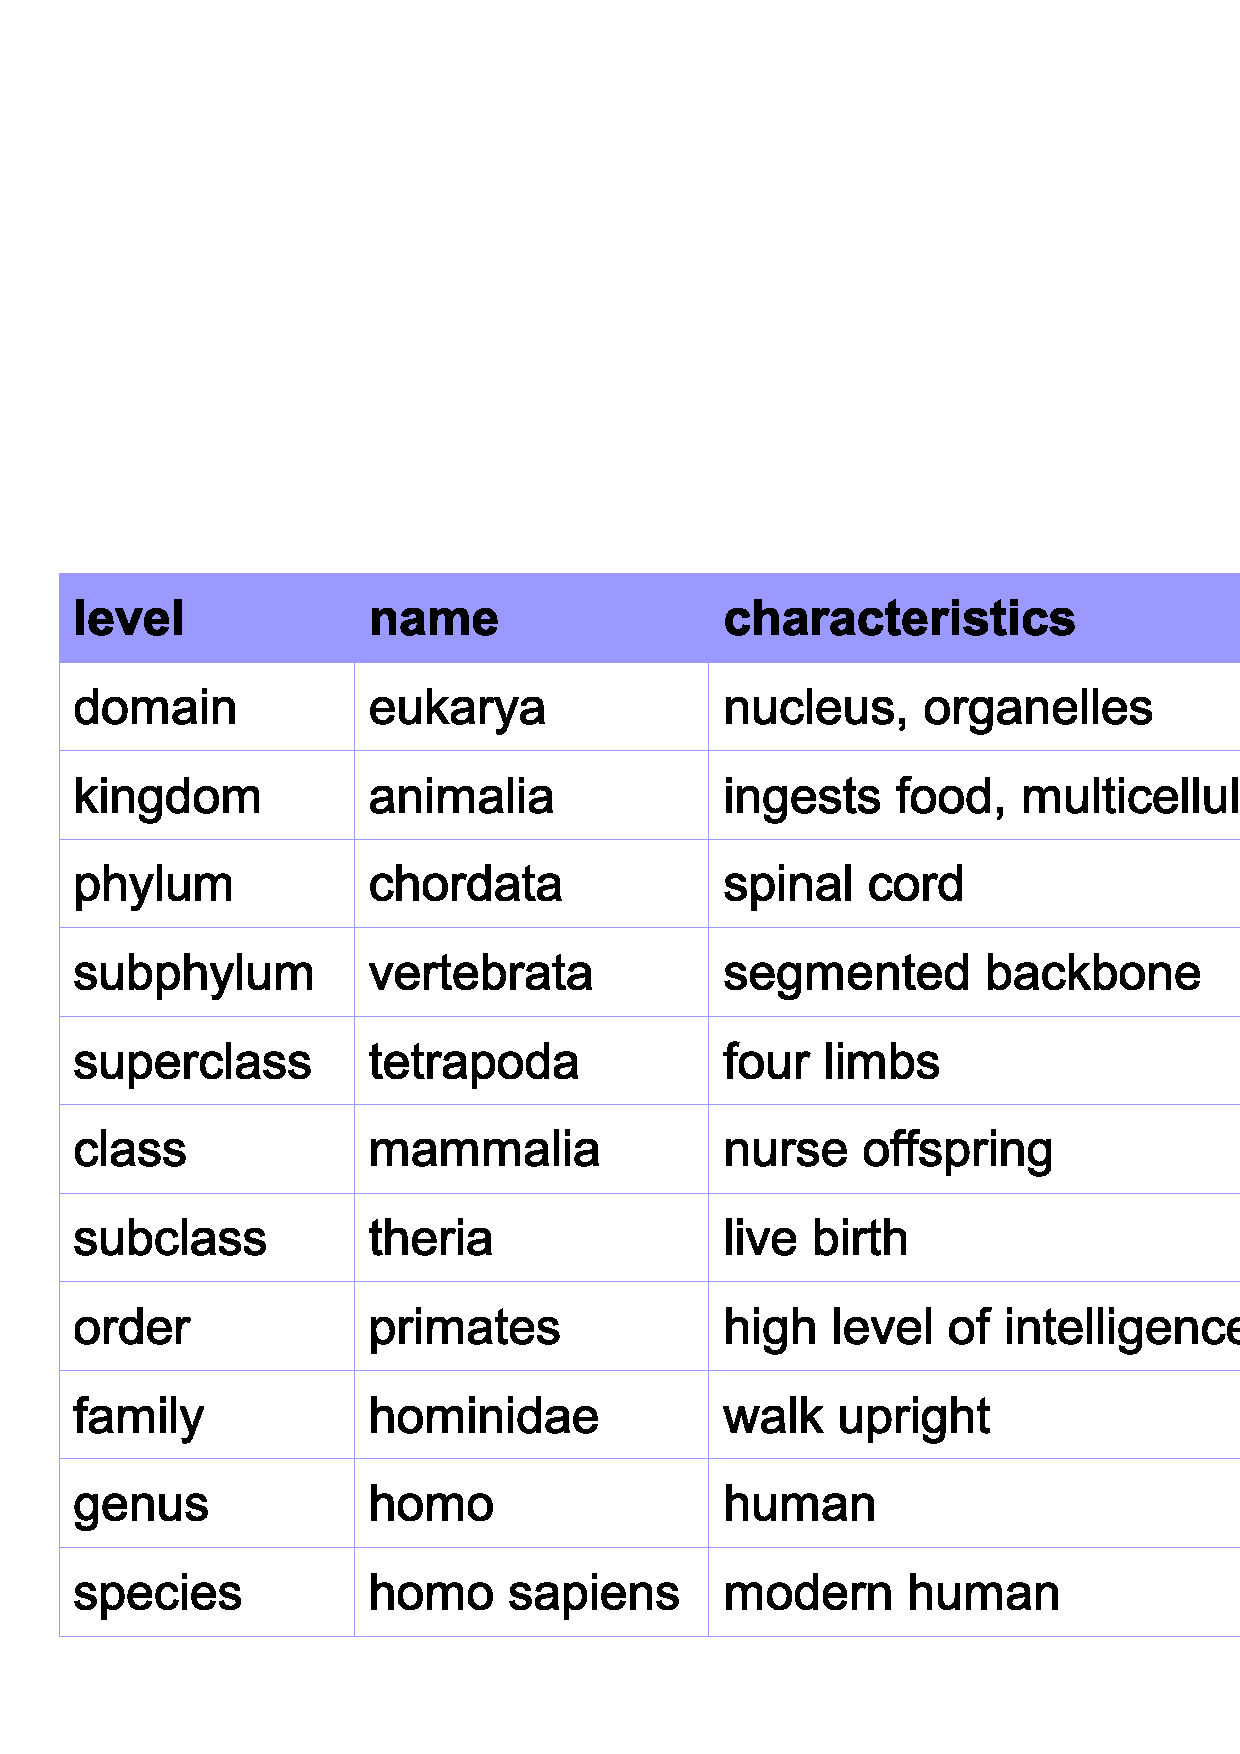
\includegraphics[scale=0.4,angle=-90]{graphic/taxonomy.pdf}
        \caption{Taxonomic Classification of the Animal Kingdom}
        \label{taxonomy_table}
    \end{center}
\end{table}

A very familiar example of an enumerated scheme is the traditional taxonomic
classification of the animal kingdom (figure \ref{taxonomy_table}). Most of the
existing medical terminologies, listing names of diseases, of surgical
operations and the like, are also enumerative. One example is the
\emph{International Classification of Diseases} (ICD) (chapter
\ref{res_medicinae_heading}).

After \cite{rogers}, attempting to enumerate in advance all useful phrases
inevitably encounters two serious problems concerning the \emph{Scale} and
\emph{Organisation}. Terminologies become:

\begin{enumerate}
    \item \emph{Scale:} too big to maintain, which results in inconsistent data
        that cannot be analysed anymore
    \item \emph{Organisation:} pre-categorised, which does not allow terms to
        be simultaneously placed under all different categories that are valid
\end{enumerate}

A further limitation is caused by unfavourable technical choices. The code often
serves two purposes. It is: the unique identifier of a concept and the means of
representing the relative organisation of a concept. So the common practice of
restricting the physical length of a code also restricts the levels of
organisation.

%
% $RCSfile: compositional_scheme.tex,v $
%
% Copyright (C) 2002-2008. Christian Heller.
%
% Permission is granted to copy, distribute and/or modify this document
% under the terms of the GNU Free Documentation License, Version 1.1 or
% any later version published by the Free Software Foundation; with no
% Invariant Sections, with no Front-Cover Texts and with no Back-Cover
% Texts. A copy of the license is included in the section entitled
% "GNU Free Documentation License".
%
% http://www.cybop.net
% - Cybernetics Oriented Programming -
%
% http://www.resmedicinae.org
% - Information in Medicine -
%
% Version: $Revision: 1.1 $ $Date: 2008-08-19 20:41:06 $ $Author: christian $
% Authors: Christian Heller <christian.heller@tuxtax.de>
%

\subsubsection{Compositional Scheme}
\label{compositional_scheme_heading}
\index{Compositional Scheme}
\index{Compositional Conceptual Scheme}
\index{Dictionary}
\index{Generalised Architecture for Languages, Encyclopedias and Nomenclatures in Med.}
\index{GALEN}
\index{Systematized Nomenclature of Medicine}
\index{SNOMED}
\index{Enumerative-compositional Scheme}
\index{Logical Observation Identifiers, Names and Codes}
\index{LOINC}
\index{International Classification of Nursing Procedures}
\index{ICNP}
\index{Combinatorial Explosion}

A \emph{Compositional Conceptual Scheme} typically contains a \emph{controlled}
and \emph{fixed} list (\emph{Dictionary}) of a relatively small number (a few
ten-thousand) of \emph{primitive} terms, each of which can have a unique code.
These primitives may be combined together by users to form more complex terms,
including those which might be found in an existing enumerative scheme but also
other, sometimes trivial, variations and expansions \cite{rogers}.

Examples of compositional schemes include the \emph{Generalised Architecture
for Languages, Encyclopaedias and Nomenclatures in Medicine} (GALEN) and the
\emph{Systematized Nomenclature of Medicine} (SNOMED). Hybrid
enumerative-compositional schemes are
\emph{Logical Observation Identifiers, Names and Codes} (LOINC) and the
\emph{International Classification of Nursing Procedures} (ICNP).

The sheer unlimited number of possible combinations, when seen as a problem, is
called \emph{Combinatorial Explosion}. Much worse problems, however, are the:

\begin{itemize}
    \item[-] \emph{Nonsense} combinations that may be constructed
        (avoidable with a set of semantic links, a grammar and constraints)
    \item[-] \emph{Redundancy} which occurs when more than one combination of
        terms express the same concept
        (avoidable with formal algorithms helping to identify redundant compositions)
    \item[-] \emph{Post-hoc Classification} (unforeseeable addition of new,
        unknown concepts) that may prevent a meaningful data analysis
        (avoidable with a type hierarchy of primitives and of semantics links)
    \item[-] \emph{Intractability} of data due to \emph{exploding} computer
        algorithms so that the computer will never find an answer
\end{itemize}

%
% $RCSfile: lexical_scheme.tex,v $
%
% Copyright (C) 2002-2008. Christian Heller.
%
% Permission is granted to copy, distribute and/or modify this document
% under the terms of the GNU Free Documentation License, Version 1.1 or
% any later version published by the Free Software Foundation; with no
% Invariant Sections, with no Front-Cover Texts and with no Back-Cover
% Texts. A copy of the license is included in the section entitled
% "GNU Free Documentation License".
%
% http://www.cybop.net
% - Cybernetics Oriented Programming -
%
% http://www.resmedicinae.org
% - Information in Medicine -
%
% Version: $Revision: 1.1 $ $Date: 2008-08-19 20:41:07 $ $Author: christian $
% Authors: Christian Heller <christian.heller@tuxtax.de>
%

\subsubsection{Lexical Scheme}
\label{lexical_scheme_heading}
\index{Lexical Scheme}
\index{Lexical Tech}
\index{Unified Medical Language System}
\index{UMLS}

A \emph{Lexical Technique} is one that helps compare phrases based on what they
appear to say -- on which words appear, in which order, and in what grammatical
constructs -- rather than on what they might or might not actually mean. Such
techniques can provide a powerful (but not 100\% accurate) method for mapping
between phrases in existing schemes, or between such phrases and the text found
in papers, the \emph{World Wide Web} (WWW) or other electronic resources.

One example of a lexical scheme is the \emph{Unified Medical Language System}
(UMLS).

Where lexical techniques break is when the language gets more \emph{slippery},
that is ambiguities may occur. Humans might interpret such results correctly,
but automated decision support systems would fail. Rogers \cite{rogers}
concludes that: \textit{As an input for autonomous machine processing
applications such as decision support, the outputs of natural language
processing tools remain unsuitable.}


%
% $RCSfile: ontology.tex,v $
%
% Copyright (c) 2001-2004. Christian Heller. All rights reserved.
%
% No copying, altering, distribution or any other actions concerning this
% document, except after explicit permission by the author!
% At some later point in time, this document is planned to be put under
% the GNU FDL license. For now, _everything_ is _restricted_ by the author.
%
% http://www.cybop.net
% - Cybernetics Oriented Programming -
%
% http://www.resmedicinae.org
% - Information in Medicine -
%
% @author Christian Heller <christian.heller@tuxtax.de>
%

\subsection{Ontology}
\label{ontology_heading}

Manifold definitions of the word \emph{Ontology} exist. They come from philosophy,
metaphysics, information technology and others -- too many to list here.
This document uses its own, adapted definition and considers an ontology to be
\emph{a strict hierarchy of abstract items, organized in levels of growing
granularity, that are solely unidirectionally related}. It such represents a
systematic description of complex domain contexts.

\begin{figure}[ht]
    \begin{center}
        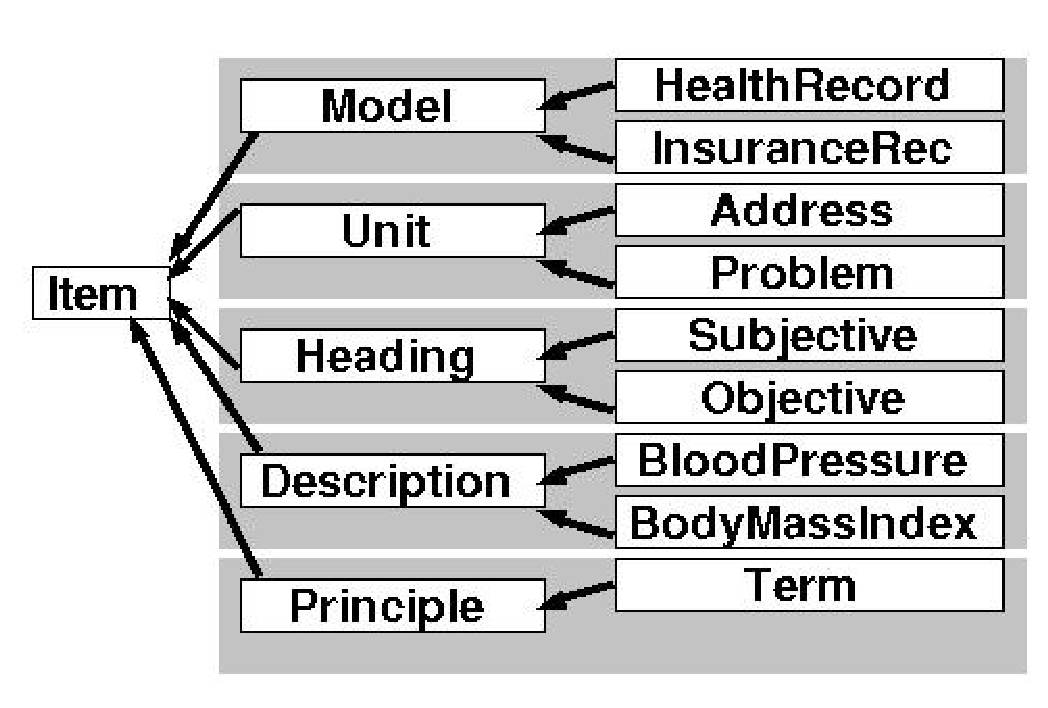
\includegraphics[scale=0.4]{vector/electronic_health_record_ontology.eps}
        \caption{Electronic Health Record Ontology}
        \label{electronic_health_record_ontology_figure}
    \end{center}
\end{figure}

Figure \ref{electronic_health_record_ontology_figure} shows one possible ontology
of an electronic health record, as described in the previous section.


%%
% $RCSfile: oio_form.tex,v $
%
% Copyright (C) 2002-2008. Christian Heller.
%
% Permission is granted to copy, distribute and/or modify this document
% under the terms of the GNU Free Documentation License, Version 1.1 or
% any later version published by the Free Software Foundation; with no
% Invariant Sections, with no Front-Cover Texts and with no Back-Cover
% Texts. A copy of the license is included in the section entitled
% "GNU Free Documentation License".
%
% http://www.cybop.net
% - Cybernetics Oriented Programming -
%
% http://www.resmedicinae.org
% - Information in Medicine -
%
% Version: $Revision: 1.1 $ $Date: 2008-08-19 20:41:07 $ $Author: christian $
% Authors: Christian Heller <christian.heller@tuxtax.de>
%

\subsection{OIO Form}
\label{oio_form_heading}

\emph{OIO Form}
Andrew Ho; OpenHealth Mailing List, December 2003 \cite{openhealth}

<form>
<item>
  <name>sBP</name>
  <description>systemic arterial blood pressure,supine</description>
  <prompt>sBP?</prompt>
  <itemtype>pressure</itemtype>
</item>
<itemtype>
  <name>pressure</name>
  <description>mmHg</description>
  <action>number</action>
  <choice></choice>
</itemtype>
</form>

OpenHealth Mailing List, December 2003 (relates to the OIO form above) \cite{openhealth}
Andrew Ho answers to Thomas Beale on the topic of OpenEHR Archetypes vs. OIO Forms

this form does not say anything about:
- systolic or diastolic (or other phases) of blood pressure
>
Just add it. Instead of "sBP" - call it "Systolic BP".
>
- what data type blood pressure is recorded as
>
The itemtype is "pressure". That is the "data type".
>
- what will you do if you want the patient standing - another form with
'standing' instead of 'supine'?
>
You can use another form or another item (a posture item).
>
- what if you want to record a time-series of BPs, say 3, with the patient
in a different position prior to each?
>
Just have 3 question items on the same form - or have 3 forms. Your choice.
>
- what if you want to record the protocol, i.e. instrument, cuff size
>
Add a question item called "protocol".
>
- how will you provide validation on data input, to e.g.
+ to ensure that
valid data types are used for each entered item (e.g. a Date is not entered
for diastolic BP)?
>
Use action=number
>
+ ensure that the systolic bp is in some sane range, e.g. 0-500mmHg?

Use action=number and choice='>20,<500', for example.
>
+ ensure that sensble positions of patient are offered to the user?

Communicate the "sensible positions" via the question prompt.
>
- how will you indicate that the data created by this form was in fact
created by this form (what is its id?), so that my software can process
the data according to the form's model of BP?
>
All data created via this OIO form are stored and labeled with the name of
this OIO form.

%
% $RCSfile: archetype.tex,v $
%
% Copyright (C) 2002-2008. Christian Heller.
%
% Permission is granted to copy, distribute and/or modify this document
% under the terms of the GNU Free Documentation License, Version 1.1 or
% any later version published by the Free Software Foundation; with no
% Invariant Sections, with no Front-Cover Texts and with no Back-Cover
% Texts. A copy of the license is included in the section entitled
% "GNU Free Documentation License".
%
% http://www.cybop.net
% - Cybernetics Oriented Programming -
%
% http://www.resmedicinae.org
% - Information in Medicine -
%
% Version: $Revision: 1.1 $ $Date: 2008-08-19 20:41:05 $ $Author: christian $
% Authors: Christian Heller <christian.heller@tuxtax.de>
%

\subsection{Archetype}
\label{archetype_heading}
\index{Archetype}
\index{Electronic Health Record}
\index{EHR}
\index{Good European/ EHR}
\index{GEHR}
\index{Open EHR}
\index{SNOMED CT}
\index{Archetype Definition Language}
\index{ADL}
\index{Constraint Form of ADL}
\index{cADL}
\index{Data Definition Form of ADL}
\index{dADL}
\index{Template Form of ADL}
\index{tADL}
\index{First Order Predicate Logic}
\index{FOPL}

With the aim of providing the means to build usable, maintainable, extensible
\emph{Electronic Health Records} (EHR), the \emph{Archetype} as design concept
was introduced in the \emph{Design Principles} document of the
\emph{Good European/ EHR} (GEHR) project, which was later renamed into
\emph{Open EHR} \cite{openehr}. Their website states: \textit{An archetype is a
re-usable, formal model of a domain concept.} Archetypes adhere to ontological
principles; they can be composed of other archetypes or atomic elements. Their
use is not limited to EHR building, despite OpenEHR's focus on the medical
domain.

Comparing archetypes with terminologies, Beale \cite{openehrtechnical} writes
that a terminology like for example SNOMED Clinical Terms (SNOMED CT) had the
form of a semantic network, i.e. \ldots\ with an ontological flavour. However,
because rigorous design principles were not always applied, they tended to be
internally inconsistent and had a lot of pre-coordination in them, while what
was really needed was a generative/ compositional terminology. Further, SNOMED
could tell what the meanings of the parts of e.g. a complete blood count test
are, but it were not going to provide a model of an actual blood test. This is
where archetypes \ldots\ would come in; they were about information
\emph{in use}, not definitions of reality (as terminologies). \ldots\ So --
even if SNOMED was perfect, it wouldn't do everything. It were a knowledge
support part of the environment, and it could be used to name things and
perform inferencing (\textit{draw a conclusion/ deduction} \cite{websters}).

An \emph{Archetype Definition Language} (ADL) \cite{adl} was created for the
specification of archetypes. A corresponding ADL document has the following
structure:

\begin{scriptsize}
    \begin{verbatim}
    archetype_id = <"some.archetype.id">
    adl_version = <"2.0">
    is_controlled = <True>
    parent_archetype_id = <"some.other.archetype.id">
    concept = <[concept_code]>
    original_language = <"lang">
    translations = <
    ...
    >
    description = <
    ...
    >
    definition = <
    cADL structural section
    >
    invariant = <
    assertions
    >
    ontology = <
    ...
    >
    revision_history = <
    ...
    >
    \end{verbatim}
\end{scriptsize}

Many separate sections can be identified in this archetype structure, and
various syntaxes are used for them. Table \ref{adl_table} gives an overview of
the structural elements of an ADL archetype. In addition to the single
sections, it mentions two further syntaxes, for templates and constraints on
data instances.

\begin{table}[ht]
    \begin{center}
        \begin{footnotesize}
        \begin{tabular}{| p{30mm} | p{30mm} | p{45mm} |}
            \hline
            \textbf{Element} & \textbf{Syntax} & \textbf{Purpose}\\
            \hline
            archetype structure & \emph{Archetype Definition Language} (ADL) & glue syntax\\
            \hline
            definition section & \emph{Constraint Form of ADL} (cADL) &
                constraints definition\\
            \hline
            description, ontology and other sections & \emph{Data Definition Form of ADL} (dADL) &
                data definition\\
            \hline
            template & \emph{Template Form of ADL} (tADL) &
                formalism to compose archetypes into larger constraint structures, used in particular contexts at runtime\\
            \hline
            data instances & \emph{First Order Predicate Logic} (FOPL) &
                constraints on data which are instances of some information model (e.g. expressed in UML)\\
            \hline
        \end{tabular}
        \end{footnotesize}
        \caption{Structural Elements of an ADL-defined Archetype \cite{adl}}
        \label{adl_table}
    \end{center}
\end{table}

Chapter \ref{cybernetics_oriented_language_heading} will define a new language
that is based on just one syntax: the \emph{Extensible Markup Language} (XML)
(section \ref{extensible_markup_language_heading}), an easy-to-grasp pure text
format. Despite its limited vocabulary of just four tags and four attributes,
that language may encode a rich set of knowledge constructs, including meta
information and constraints.

%
% $RCSfile: dual_model_approach.tex,v $
%
% Copyright (C) 2002-2008. Christian Heller.
%
% Permission is granted to copy, distribute and/or modify this document
% under the terms of the GNU Free Documentation License, Version 1.1 or
% any later version published by the Free Software Foundation; with no
% Invariant Sections, with no Front-Cover Texts and with no Back-Cover
% Texts. A copy of the license is included in the section entitled
% "GNU Free Documentation License".
%
% http://www.cybop.net
% - Cybernetics Oriented Programming -
%
% http://www.resmedicinae.org
% - Information in Medicine -
%
% Version: $Revision: 1.1 $ $Date: 2008-08-19 20:41:06 $ $Author: christian $
% Authors: Christian Heller <christian.heller@tuxtax.de>
%

\subsection{Dual Model Approach}
\label{dual_model_approach_heading}
\index{Dual Model Approach}
\index{Analysis Pattern}
\index{Two Level Modelling}
\index{Knowledge Level}
\index{Operational Level}
\index{Reflection Pattern}
\index{Meta Level}
\index{Base Level}
\index{Archetype Model}
\index{AM}
\index{Reference Model}
\index{RM}
\index{ADL}
\index{OpenEHR}

The idea of archetypes was inspired by Martin Fowler's \emph{Analysis Patterns}
\cite{fowler1997} describing a kind of ad hoc two-level modelling, using a
\emph{Knowledge Level} and \emph{Operational Level} -- as described by the
\emph{Reflection} pattern (section \ref{reflection_heading}), which calls the
two levels \emph{Meta Level} and \emph{Base Level}, respectively. Fowler tried
to put as much general domain knowledge as possible into the meta level, in
order to make application systems more flexible, and to remove unnecessary
dependencies. Archetypes represent what would traditionally have been put into
the knowledge (meta) level.

Because an \emph{Archetype Model} (AM) (defined in form of ADL documents) and
its runtime instances constrain a \emph{Reference Model} (RM) and its instances
(figure \ref{dual_figure}), development with archetypes is called the
\emph{Dual Model Approach} \cite{openehr}. Archetypes represent the knowledge
belonging to the meta level; the reference model contains information belonging
to the base level. \textit{RMs are domain-invariant, i.e. the concepts
expressed in the base models mean the same thing right across the domain.}
\cite[Beale]{openehrtechnical}

\begin{figure}[ht]
    \begin{center}
        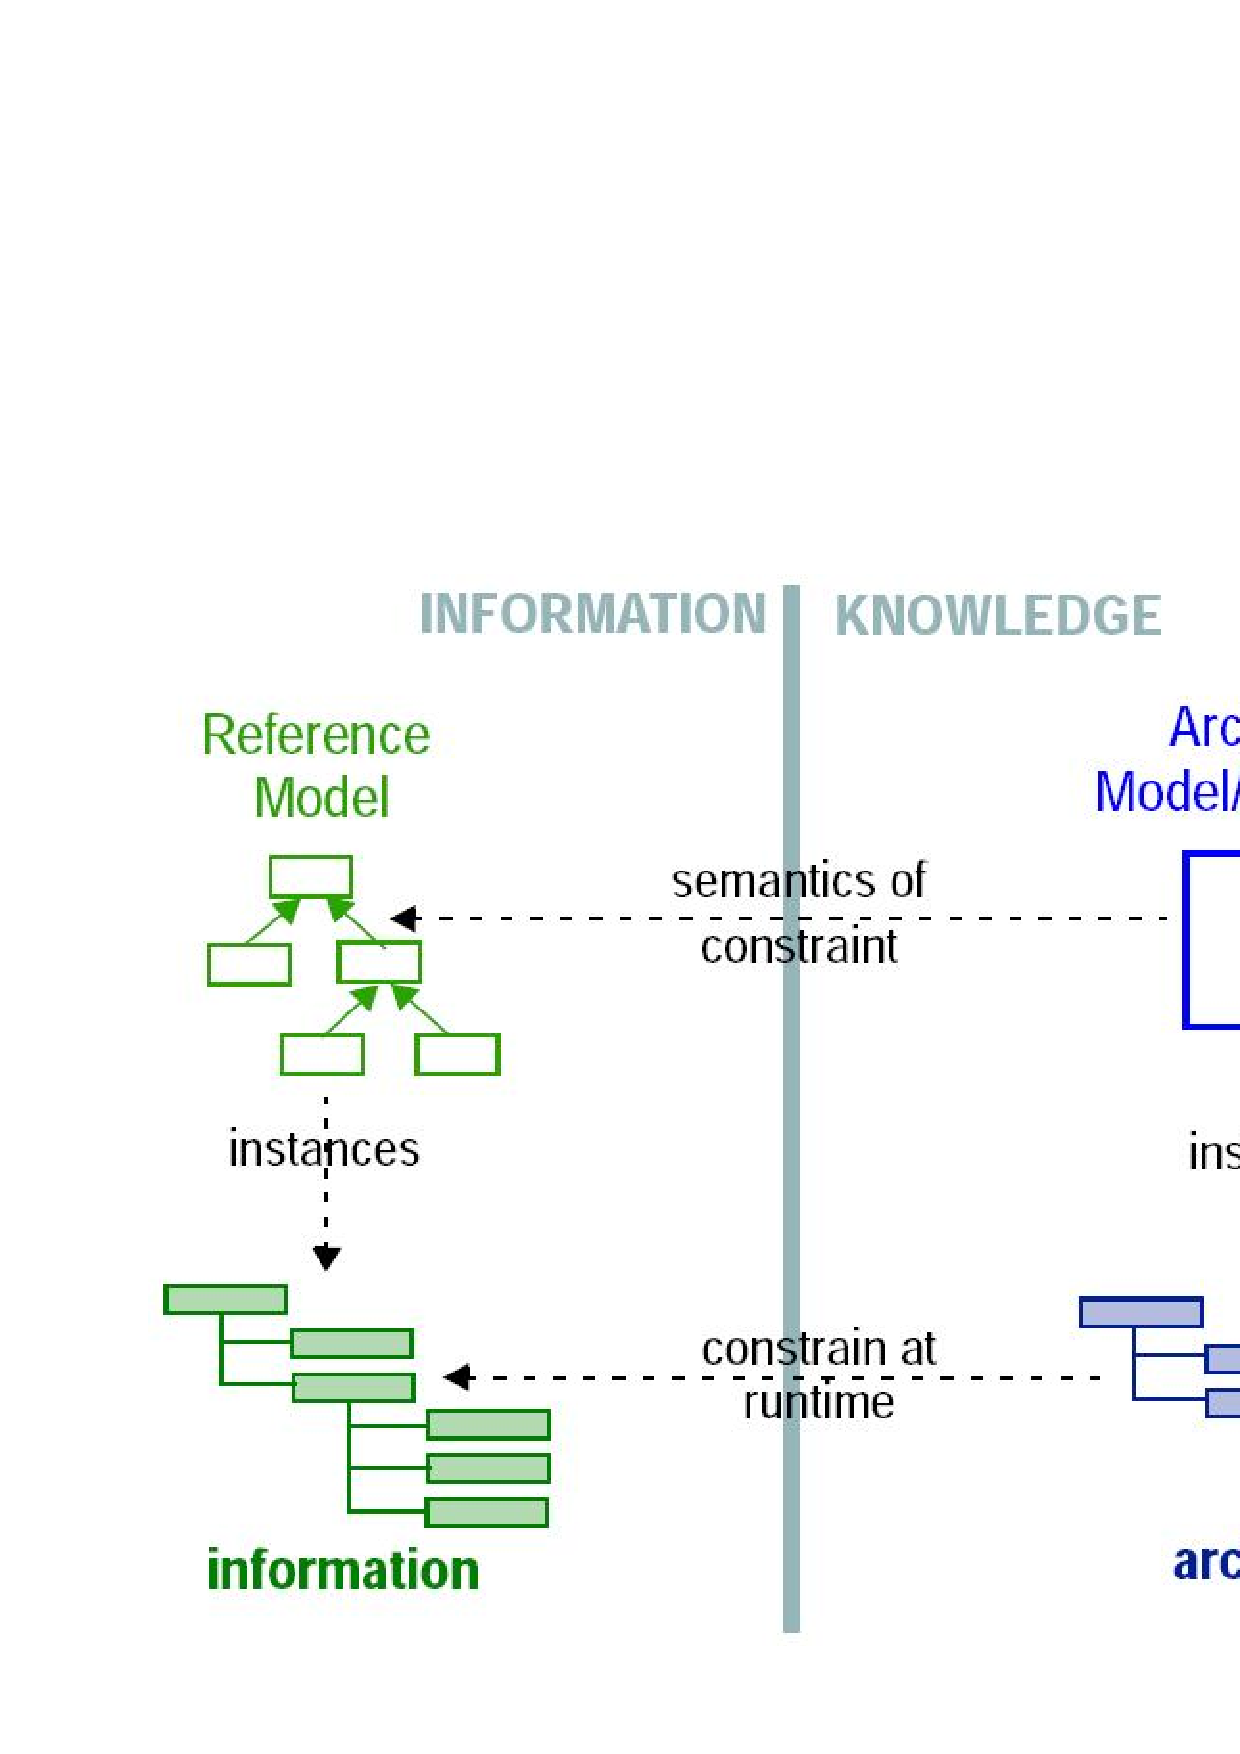
\includegraphics[scale=0.3,angle=-90]{graphic/dual.pdf}
        \caption{Dual Model Approach \cite{archetypes}}
        \label{dual_figure}
    \end{center}
\end{figure}

The difference between the dual model approach and classical meta architectures
is that the latter implement both, meta- and base level using the same
technology (language). Archetypes, on the other hand, use the ADL for
specifying knowledge. Further, the AM does not depend on the RM, as opposed to
meta architectures, where both models depend on each other bidirectionally.
Ergo, the dual model approach is rather comparable to \emph{Agents} (section
\ref{agent_oriented_programming_heading}) owning a mental state (knowledge base).

There are unclear views on what exactly should be constrained when. Sam Heard
\cite{openehrtechnical} writes about an \emph{Archetype Kernel} -- a tool that
could help build (knowledge instances) and ensure that (they) comply to
archetypes \ldots\ It could operate at a range of points, at:

\begin{itemize}
    \item[a] write and edit time: allowing constraint of the data to be based
        on archetypes (metadata) rather than application specific processes;
    \item[b] creation time of the application or schema: so that the
        application has read all information constraining the data as indicated
        -- but not through interaction with the archetype at runtime;
    \item[c] persistence time: into a database or some other persistence means;
    \item[d] communication time: such as when creating a model extract.
\end{itemize}

Besides obvious benefits of these approaches in constraining domain knowledge,
there are a number of potential problems, as Heard mentions:

\begin{quote}
    \emph{a} makes \emph{b} and \emph{c} redundant and allows the application
    to stay up to date with the archetype development process; \emph{b} makes
    \emph{c} redundant (potentially) but means code has to be cut to
    encorporate new archetypes; \emph{c} and \emph{d} mean that data may be
    proved incompatible at a time later than data entry and this may lead to
    other problems; \emph{d} means you can carry on regardless but there is a
    risk that data collected will not be compatible with models that are
    proposed for interoperability.
\end{quote}

Further weaknesses of archetypes, the ADL and dual model approach are:

\begin{itemize}
    \item[-] mix of meta information (properties, constraints) and hierarchical whole-part structure in ADL
    \item[-] incomplete domain knowledge in ADL lacking logic (algorithms/ workflows) and user interfaces
    \item[-] inflexible structures due to runtime-dependency of RM instances from archetypes
    \item[-] use of object-oriented concepts with all their limits, for RM as well as for AM instances
\end{itemize}

Although the \emph{OpenEHR} project \cite{openehr} claims archetypes to be both:

\begin{enumerate}
    \item[-] \emph{domain-empowered:} domain experts, rather than information
        technology people, become able to directly define and manage the
        knowledge definitions of their systems;
    \item[-] \emph{future-proof:} systems can be deployed prior to having
        created formal knowledge models of the (entire) domain
\end{enumerate}

\ldots\ the above-mentioned issues prevent them from being so. The dual model
approach in conjunction with archetypes only partly fulfills the expectations
of independent and complete knowledge structures. CYBOP sets out to solve these
issues and to find a truely future-proof, long-life system architecture.
Knowledge templates written in the language described later in this work
(chapter \ref{cybernetics_oriented_language_heading}) may not only contain meta
information constraining application models (as archetypes do), they represent
the application itself. The templates themselves are constrained at design time
through one universal knowledge schema (chapter \ref{knowledge_schema_heading})
dictating their structure. Runtime knowledge models do not reference the
template they were instantiated with (contrary to RM instances referencing
their corresponding AM instance); a CYBOP application holds all constraints
directly in its knowledge models (runtime instances). Since these models follow
the structure of the singular knowledge schema as well, they can be serialised
easily what makes further constrain activities for persistence or communication
unnecessary.


%%
% $RCSfile: xml_based_programming.tex,v $
%
% Copyright (C) 2002-2008. Christian Heller.
%
% Permission is granted to copy, distribute and/or modify this document
% under the terms of the GNU Free Documentation License, Version 1.1 or
% any later version published by the Free Software Foundation; with no
% Invariant Sections, with no Front-Cover Texts and with no Back-Cover
% Texts. A copy of the license is included in the section entitled
% "GNU Free Documentation License".
%
% http://www.cybop.net
% - Cybernetics Oriented Programming -
%
% http://www.resmedicinae.org
% - Information in Medicine -
%
% Version: $Revision: 1.1 $ $Date: 2008-08-19 20:41:09 $ $Author: christian $
% Authors: Christian Heller <christian.heller@tuxtax.de>
%

\section{XML Based Programming}
\label{xml_based_programming_heading}

%
% $RCSfile: user_interface_modelling.tex,v $
%
% Copyright (C) 2002-2008. Christian Heller.
%
% Permission is granted to copy, distribute and/or modify this document
% under the terms of the GNU Free Documentation License, Version 1.1 or
% any later version published by the Free Software Foundation; with no
% Invariant Sections, with no Front-Cover Texts and with no Back-Cover
% Texts. A copy of the license is included in the section entitled
% "GNU Free Documentation License".
%
% http://www.cybop.net
% - Cybernetics Oriented Programming -
%
% http://www.resmedicinae.org
% - Information in Medicine -
%
% Version: $Revision: 1.1 $ $Date: 2008-08-19 20:41:09 $ $Author: christian $
% Authors: Christian Heller <christian.heller@tuxtax.de>
%

\subsection{User Interface Modelling}
\label{user_interface_modelling_heading}

- GUIs bisher nie einheitlich beschrieben wie RDB mit ERM und DDL/SQL
- jetzt erst erreichen GUIs mit der UIML den Stand von DDL/SQL
- so wie RDBMS durch OODBMS ersetzt wurden und damit entfielen,
OODBMS mit OO Domain Layer verschmolzen ist, kann evtl. auch das GUI
mit der Domain verschmolzen werden! ==> NEIN! weil Domain Daten unterschiedlich
im GUI dargestellt werden koennen (Edit, Liste, Tabelle, Tree) und Anwender
verschiedene Wuensche und Anforderungen an das GUI haben, weswegen die Entwickler
die GUIs flexibel erstellen und handhaben muessen, was nicht gegeben waere,
wenn das GUI vom DomainModel fest vorgegeben waere

Common libraries used for data display design are the \emph{GIMP Toolkit} (GTK)
of the \emph{General (GNU) Image Manipulation Program} (GIMP) and the \emph{Qt Toolkit},
both written in C++, as well as the \emph{Abstract Window Toolkit} (AWT)/ \emph{Swing}
for Java.

mention and shortly describe \emph{GUI Renderer} (section pattern_merger refers to here)

\input{bean}
\input{xml_user_interface_language}
%
% $RCSfile: user_interface_markup_language.tex,v $
%
% Copyright (C) 2002-2008. Christian Heller.
%
% Permission is granted to copy, distribute and/or modify this document
% under the terms of the GNU Free Documentation License, Version 1.1 or
% any later version published by the Free Software Foundation; with no
% Invariant Sections, with no Front-Cover Texts and with no Back-Cover
% Texts. A copy of the license is included in the section entitled
% "GNU Free Documentation License".
%
% http://www.cybop.net
% - Cybernetics Oriented Programming -
%
% http://www.resmedicinae.org
% - Information in Medicine -
%
% Version: $Revision: 1.1 $ $Date: 2008-08-19 20:41:09 $ $Author: christian $
% Authors: Christian Heller <christian.heller@tuxtax.de>
%

\subsubsection{User Interface Markup Language}
\label{user_interface_markup_language_heading}

User Interface Markup Language (UIML)


%
% $RCSfile: workflow.tex,v $
%
% Copyright (C) 2002-2008. Christian Heller.
%
% Permission is granted to copy, distribute and/or modify this document
% under the terms of the GNU Free Documentation License, Version 1.1 or
% any later version published by the Free Software Foundation; with no
% Invariant Sections, with no Front-Cover Texts and with no Back-Cover
% Texts. A copy of the license is included in the section entitled
% "GNU Free Documentation License".
%
% http://www.cybop.net
% - Cybernetics Oriented Programming -
%
% http://www.resmedicinae.org
% - Information in Medicine -
%
% Version: $Revision: 1.1 $ $Date: 2008-08-19 20:41:09 $ $Author: christian $
% Authors: Christian Heller <christian.heller@tuxtax.de>
%

\subsection{Workflow}
\label{workflow_heading}

\input{pipeline_and_pipelet}
\input{open_infrastructure_for_outcomes}
many UNIX commands which are connected by many pipes and such form a pipeline

http://openflow.sourceforge.net/index.html
"Welcome to the home page of the OpenFlow Project. OpenFlow aims to
build a workflow and document flow management system for the Italian
Public Administration."
They don't seem to have any code available yet and some of the dates
stem from 1993!

wftk: Open-source workflow toolkit http://www.vivtek.com/wftk/
this work was paid for via collabnet.  This is a C implementation.

Micro-Workflow: http://micro-workflow.com/Research/  Started off as an
academic project, the example on this page is medically oriented.  Open
source might be coming however as the author states: "My plan is to give
out the framework under the terms of the GNU General Public License.
Currently I am working on cleaning up the code. As soon as I'm through I
will make it available from these Web pages."

I can't really verify this, but at one time I read the the OMG jFlow
workflow service was being added to  the open source real-time ORB
project TAO here:
http://www.cs.wustl.edu/~schmidt/TAO-status.html

DSTC's Elvin project: http://elvin.dstc.edu.au/intro/overview.html
While described as \textit{a content-based routing service}, there are workflow
aspects to this software.  I would think that content-based routing
would be very interesting to medical software folks.  My plan is to
start experimenting with Elvin after our content managment system comes
on-line (the RFP mentioned above).

Bud P. Bruegger \cite{openoutcomesgeneral}
Thanks for the pointer to the overview paper on PROforma--definitely the
best of all I've seen.

At 01:24 PM 14-03-01 -0800, Andrew po-jung Ho wrote:
>In summary, PROforma looks promising and not overly complex. It could be a
>good standard for Openflow and OIO to consider adopting. Since I don't
>have much experience with workflow systems, I look forward to you, Paolo,
>and other list member's guidance.

In the following are some thoughts on PROforma and workflow models in
general.  They are based on a still incomplete understanding of the
situation, but maybe it can help bring the discussion further.

It seems to me that PROforma is highly specialized and far from a general
purpose workflow model.  Also, apart from workflow, it deals a lot with
decision support.  Something that general purpose workflow systems usually
have but that I didn't find in PROforma (did I miss it?) is a description
of how work flows withing a group of people.  A typical example in an
administrative organisation would be a document/application/etc. to flow
between people of different roles, each of whom add their contribution...

PROforma seems so specialized to clinical decision support that I wonder
whether it would be applicable as a workflow component in a LIMS.

So what workflow model/component to use???  A difficult question.  I looked
around quite a bit so far and haven't found a single thing that convinces
me all the way (obviously for my purposes).

On the standard side, I'm not convinced that the WfMC or OMG standards are
really the way to go  (look at the critique by the former IETF SWAP leader
that I sent you earlier--I don't think these things have really been
addressed by WfMG's new wf-XML that does not seem to break with the
problematic reference model).

I spent quite some time reading agent-technology workflow papers and non of
these people seems to even look at the WfMG standards.  It seems they use
petri-nets and similar as models and some use some other process
description standards (that probably are mostly relevant to manufacturing).

So unless there is a strong need for interoperation with a WfMG standard
complient external workflow system, I'm not sure wether it's worth the
effort of adding the effort and complexity that comes with the standard.

Other features that are not standardised seem much more important to
me.  For example, the possibility to negotiate as it is typical for
agent-based approaches. (As mentioned in section 8.2 of
http://www.acl.icnet.uk/PUBLICATIONS/ms364.pdf that you pointed
out).  Also, a peer-to-peer architecture that allows collaboration and
scalability way beyond the boundaries of a singe administrative
control.  Such features seems to be almost incompatible with the current
standards.

Going to actually available systems, my impression is that there are
roughly three categories of systems that call themselves "workflow" systems:

1. Task-Management systems such as those used in Ticket tracking and
help-desk systems.  Their basic entity is a task.  The notion of "flow"
comes in through the possibility of defining task dependencies.  But this
is very cumbersome and way too limited for many kinds of workflow needs.

Typically, these systems assign human resources to tasks (who is
responsible for execution, who created the task), but lack any notion of
other resources, such as for example documents that "flow" around in the
work process.  (To be fair, some deal with descriptions of the task coming
via e-mail etc.--but that's very specialized and not general at all).

2. Workflow systems that model an actual flow of tasks by connecting tasks
in some kind of a graph.  Most serious workflow systems and the WfMG model
fall into this category.

There is probably a major difference of how systems deal with resources
that are relevant to work processes.  All systems probably model human
resources.  Most systems (but not all) allow you that tasks reference their
input and output resources.  IMO, the mechanism of referencing resources
from task makes it difficult to understand the flow of resources
(documents, data) in the workflow.  I personally believe that models that
emphasise tasks at the cost of resources can be rather limited in some
kinds of workflow applications (such as LIMS) where resources (eg. samples
and specimen in a LIMS) are first class citizens.

3. There seems to be a few workflow systems that model workflow as complete
graphs and also treat resources as first class citizens.  This was my naive
idea (before I looked into workflow systems in more detail) of a workflow
component for a LIMS (see
http://www.sistema.it/labinfo/single.html#Relationships between Entities)
but also seems to be used by systems such as PIPER
(http://bioinformatics.org/piper/) and Khoros
(http://www.khoral.com/ideas/technology/cantata.pdf).

Piper actually looks VERY interesting but it seems too early to be used
(still alpha).  Interesting that Piper does not seem to bother about any
workflow standard.  I suppose that treating resources as first-class
citizens may be incompatible with the WfMG approach.  (Interesting for the
OIO folks is that the upper layers of Piper are written in Python).

Another product that may be able to manage workflows is the Narval software
agent (http://www.logilab.org/narval/).  <quote>Narval is the acronym of
"Network Assistant Reasoning with a Validating Agent Language". It is a
personal network assistant based on artificial intelligence and agent
technologies. It executes recipes (sequences of actions) to perform tasks.
It is easy to specify a new action using XML and to implement it using
Python. Recipes can be built and debugged using a graphical
interface.  </quote>

It has been used to automate some special workflows (eg the translation of
Linux Gazette to French
http://www.linuxgazette.com/issue59/chauvat.html).  It is written in Python
and seems to be quite user-friendly and easy to program  (as compared to
some Java agent systems).  I think it may be worth while to look into
Narval (and a different paradigm of thinking) to see how that would be
applicable to workflow in healthcare applications.  My gutt feeling is
quite positive...

Workflow
http://sourceforge.net/projects/tikiwiki/


- in Microsoft Windows "Longhorn": Win-FX XAML (YAML??)
http://www.ondotnet.com/pub/a/dotnet/2004/01/19/longhorn.html
http://www.codeproject.com/csharp/treemaps.asp
\cite{xaml}
http://www.xaml.net/

- ebXML (with OWL support??, by Sun Microsystems)
- W3C XForms

Extensible Programming for the 21st Century/ XML Based Programming \cite{wilson}:
- suggests to put an additional layer of abstraction (in XML) on top of current
programming languages
- programmers would be able to customise their "views" of software without
modifying the underlying model

"We believe that next-generation programming systems will store source code as XML,
rather than as flat text. Programmers will not see or edit XML tags; instead, their
editors will render these models to create human-friendly views, just as web browsers
render HTML. For example, a program might be stored on disk like this:"

<doc>Only replace below threshold</doc>
<cond>
  <test>
    <compare-expr operator="less">
      <field-expr field="age"><evaluate>record</evaluate></field-expr>
      <evaluate>threshold</evaluate>
    </compare-expr>
  </test>
  <body>
    <invoke-expr method="release"><evaluate>record</evaluate></invoke-expr>
  </body>
</cond>

- would be viewed and edited like this:

// Only replace below threshold
if (record.age < threshold) {
    record.release();
}

or:

if (record.age < threshold)    /* Only replace below threshold */
{
        record.release();
}

or even this (Scheme language):

;;; Only replace below threshold
(if (< (record 'age) threshold)
    (record 'release))

%
% $RCSfile: modelling_mistakes.tex,v $
%
% Copyright (c) 2005-2006. Christian Heller. All rights reserved.
%
% Permission is granted to copy, distribute and/or modify this document
% under the terms of the GNU Free Documentation License, Version 1.1 or
% any later version published by the Free Software Foundation; with no
% Invariant Sections, with no Front-Cover Texts and with no Back-Cover
% Texts. A copy of the license is included in the section entitled
% "GNU Free Documentation License".
%
% http://www.cybop.net
% - Cybernetics Oriented Programming -
%
% http://www.resmedicinae.org
% - Information in Medicine -
%
% Version: $Revision: 1.1 $ $Date: 2006-01-03 08:21:45 $ $Author: christian $
% Authors: Christian Heller <christian.heller@tuxtax.de>
%

\subsection{Modelling Mistakes}
\label{modelling_mistakes_heading}

Most modern software is not written directly in a machine language but designed
in form of higher-level models instead. These allow to speed up application
development and help avoiding errors. \emph{Object Oriented Programming} (OOP),
for example, uses design concepts like the \emph{Class} owning \emph{Attributes}
and \emph{Methods}. Yet does this kind of modelling create abstractions that
reflect concepts of the real world completely and correctly?

\begin{figure}[ht]
    \begin{center}
        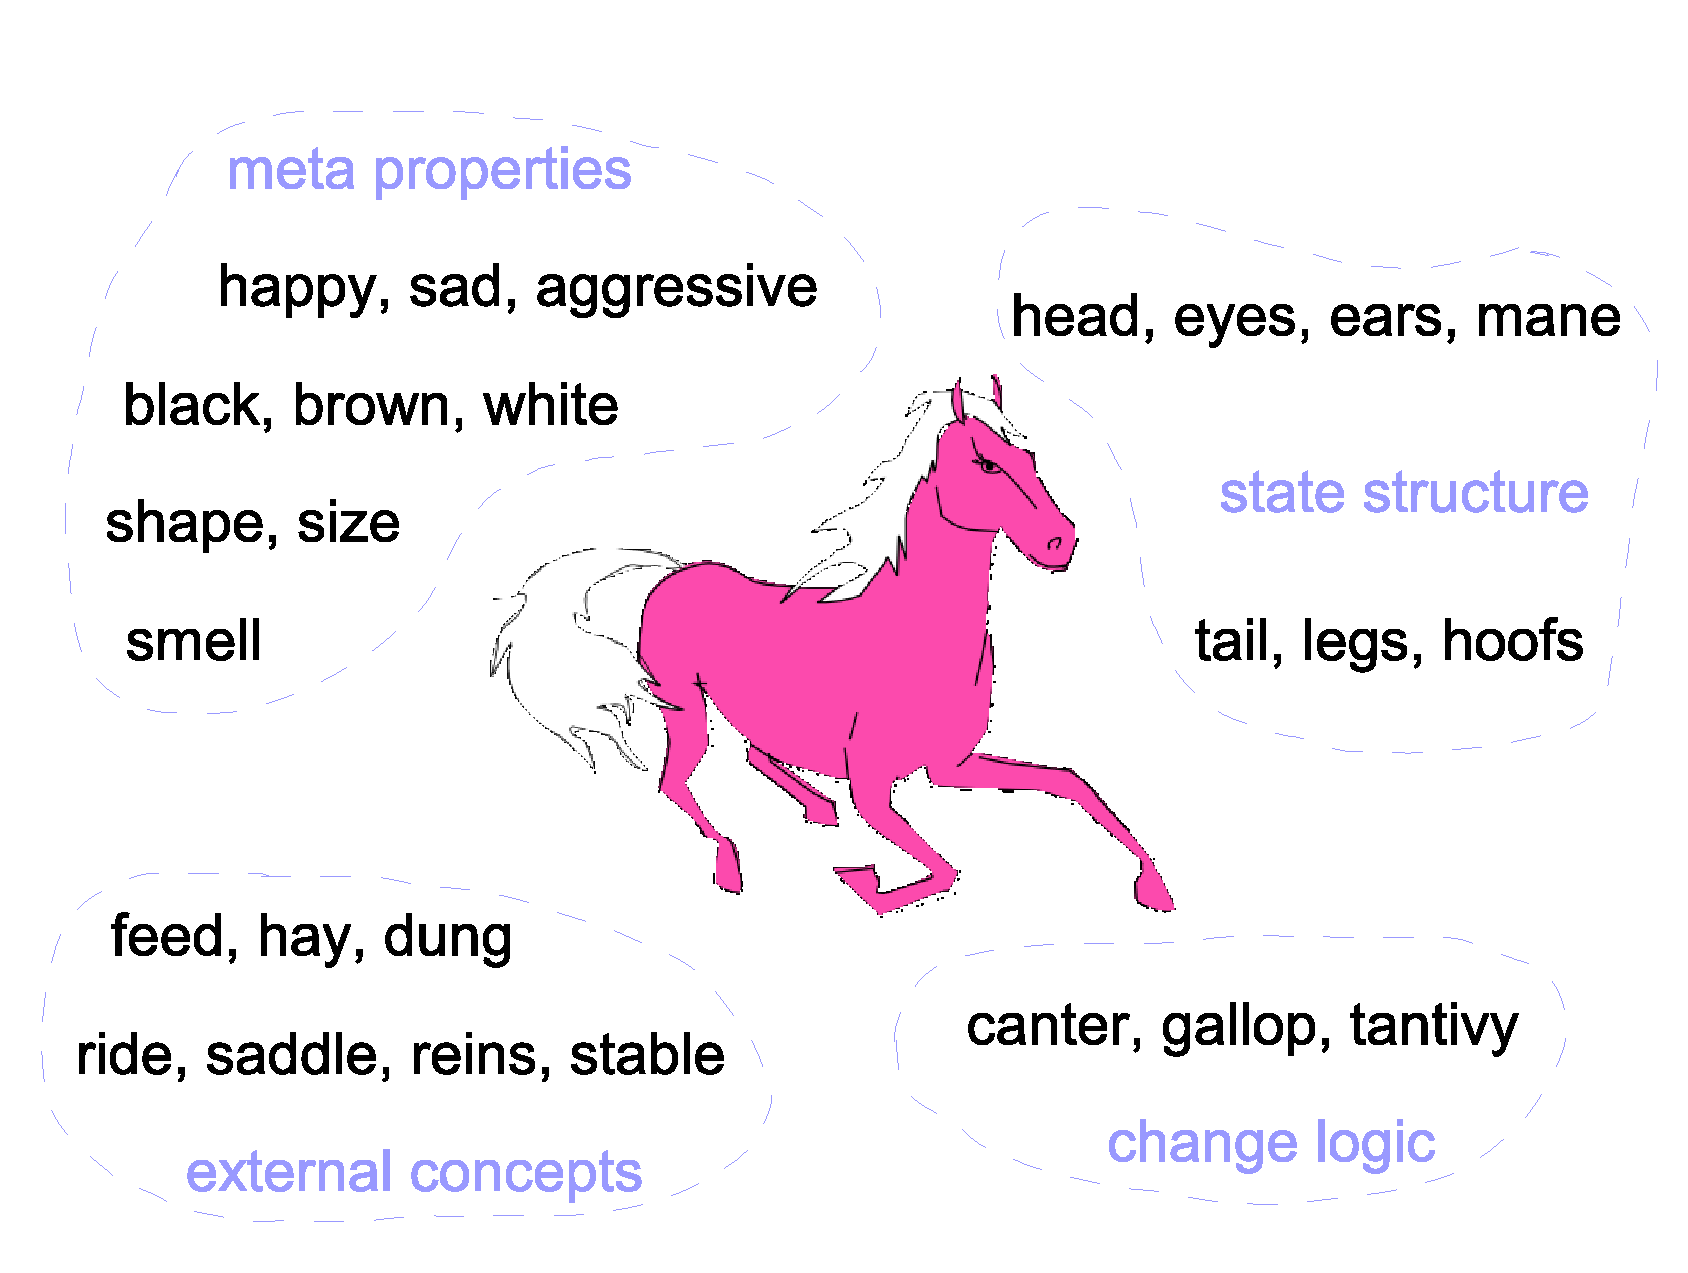
\includegraphics[scale=0.2]{vector/horse.eps}
        \caption{Concept of a Horse}
        \label{horse_figure}
    \end{center}
\end{figure}

The model of a \emph{Horse} shall serve as example to investigate this further.
Figure \ref{horse_figure} shows a number of terms commonly used to describe a
horse. Most importantly, there are structural observations describing the horse
as concept consisting of parts like \emph{Head}, \emph{Legs} or \emph{Hoofs}.
Secondly, there are properties like the horse's \emph{Colour}, \emph{Shape} or
\emph{Size}. Thirdly, there are terms describing a horse's actions like its
\emph{Movement} or \emph{Eating}, that change a horse's position and/ or state.
Finally, there are a number of terms like \emph{Hay} or \emph{Saddle}
associating concepts related to the horse.

One might suggest to model properties like the position, size or colour of a
horse's leg as \emph{Part} of that leg. In fact, this is how classical
programming approaches its solutions. In OOP, one would probably use a class
representing the leg and an attribute standing for the leg's colour. However,
when following the modelling principles of human thinking (see
\cite{heller2004}), this is \emph{not} correct!

It is true that in everyday language, one tends to say \textit{A horse leg
\emph{has a} colour.} Unfortunately, this leads to the wrong assumption that a
leg were made of a colour. But this is not the case. A leg does not
\emph{consist} of a colour in the hierarchical meaning of a whole consisting of
parts. The colour is rather property information \emph{about} the leg. It seems
there is no correct expression in natural (English) language stating the
property of something. The \emph{IS-A} verbalisation is used to express that
the leg belongs to a special category of items, for example: \textit{A leg is a
body element.} The \emph{HAS-A} formulation is used to express that a leg as
whole consists of smaller parts, for example: \textit{A leg has a knee and it
has a hoof.} But which formulation expresses a property? Well, perhaps it would
be best to say: \textit{A leg IS-OF a colour.}

The CYBOP knowledge schema described later in this article distinguishes
structural- from meta information. Actions (like the gallop of a horse) causing
change in the model or its environment are called \emph{Logic} in this work,
since they follow certain rules.

